\documentclass[a4paper,11pt,danish,twoside,openany]{look/05gr551c} % Sideopstning (openany starter et nyt kapitel p vilkrlig side)openright aabner paa hoejre side mvh Per


%  Sideopstning inkl.  margin mm. 
\usepackage{anysize}	              % Set margin sizes with simple commands.
\usepackage{geometry}									%LOLOLOLOLLLLL######
\marginsize{4cm}{5cm}{2.9 cm}{2.9 cm}		% Definerer strrelse af marginer
\usepackage{setspace}										% Mulighed for dobbelt linieafstand
\usepackage[makeroom]{cancel}

\usepackage{transparent}

%Akronymliste
\usepackage[intoc]{nomencl}
\renewcommand{\nomname}{Symbol- and Acronym List}

%\makeatletter
%    \def\thenomenclature{%
%      \@ifundefined{chapter}%
%      {
%        \section*{\nomname}
%        \if@intoc\addcontentsline{toc}{section}{\nomname}\fi%
%      }%
%      {
%        \chapter*{\nomname}
%        \if@intoc\addcontentsline{toc}{chapter}{\nomname}\fi%
%      }%
%
%      \nompreamble
%      \list{}{%
%        \labelwidth\nom@tempdim
%        \leftmargin=0pt
%        \itemindent=\dimexpr\itemsep+\labelwidth\relax
%        \itemsep\nomitemsep
%        \let\makelabel\nomlabel}}
%    \makeatother

\makenomenclature
% Kr�ver at man i terminalen skriver:
%
% makeindex filename.nlo  -s nomencl.ist -o filename.nls
%
% for at printnomenclature i Rapport.tex tager input ind p� listen.
% Der oprettes et punkt p� listen et vilk�rligt sted (sammen med 
% forkortelsen er n�vnt f�rste gang) ved at inds�tte f�lgende:
%
% \nomenclature[prefix]{symbol}{description} 
% hvor prefix er optional, symbol er forkortelsen, description er det den st�r for

% This prints the Nomenclature in two columns % % % % % % % % % % % % % % % %
\usepackage{multicol}
\makeatletter
\@ifundefined{chapter}
  {\def\wilh@nomsection{section}}
  {\def\wilh@nomsection{chapter}}  
\def\thenomenclature{%
  \begin{multicols}{2}[%  
    \csname\wilh@nomsection\endcsname*{\nomname}
    \if@intoc\addcontentsline{toc}{\wilh@nomsection}{\nomname}\fi
    \nompreamble]
  \list{}{%
    \labelwidth\nom@tempdim
    \leftmargin\labelwidth
    \advance\leftmargin\labelsep
    \itemsep\nomitemsep
    \let\makelabel\nomlabel}%
}
\def\endthenomenclature{%
  \endlist
  \end{multicols}
  \nompostamble}
\makeatother

% % % % % % % % % % % % % % % % % % % % % % % % % % % % % % % % % % % %

\setlength{\columnsep}{1.8em}	% specifies the margin (space) between columns in the nomenclature
\setlength{\nomitemsep}{0.01cm} % specifies the space between item and explanation in the nomenclature

% Makes it possible to specify unit inside nomenclature environment with nomunit
\newcommand{\nomunit}[1]{%
\renewcommand{\nomentryend}{\hspace*{\fill}#1}}


%Appendixops�tning
\usepackage[toc,page,titletoc]{appendix}
\renewcommand{\appendixname}{Appendix}
\renewcommand{\appendixtocname}{Appendix}
\appendixpageoff
\appendixheaderon
\appendixtocoff
\appendixtitletocon
\appendixtitleon



%  Oversttelse og tegnstning 
\usepackage{t1enc}											% Hjlper med orddeling ved ,  og .
\usepackage[english]{babel} 							% Dansk sprog, bl.a. figure bliver til figur
%\usepackage[latin1]{inputenc}					% Gr det muligt at bruge ,  og  i sine .tex-filer
\usepackage[ansinew]{inputenc}					% Gr det muligt at bruge ,  og  i sine .tex-filer
\usepackage[T1]{fontenc}						% Giver flere mulige karakterer, s� fx � er �n karakter i stedet for to best�ende af o og �
\usepackage{latexsym}										% LaTeX symboler
\usepackage{ragged2e}										% Gr det mulig at venstre-/hjrecentrere blokke
\usepackage{import}					%For at importere svg med latex font
\usepackage{longtable}

%  Figurer og tabeller  floats  
%\usepackage{look/svg}	%makes it possible to define height of pdf_tex files for use in subfigure
\usepackage{graphicx} %til Matlab%
\usepackage{grffile}  %til Matlab%


\usepackage{subfigure}               		% Til at stte flere underfigurer med hver sin caption ind i samme figur.
%\usepackage{subfig}
%\renewcommand{\thesubtable}{\arabic{subtable}}
%\captionsetup[subtable]{labelformat=empty}
\usepackage{sidecap} 										% Caption ved siden af figurer / tabellen.




\usepackage{flafter}										% Srger for at dine floats ikke optrderi texten fr de er sat ind.
\usepackage{tabularx}										% Muliggr at angive bredden af tabellen.
\newcolumntype{L}{>{\raggedright\arraybackslash}X}			% venstrejustering i tabularx (L=X)
\newcolumntype{R}{>{\raggedleft\arraybackslash}X}			% G�r det muligt at h�jrejustere i tabularx
\usepackage{float}											% Forbedrer samspillet mellem defineringer af flydende objekter.
\usepackage{longtable}									% Gr s tabeller lettere kan strkke sig over flere sider

\usepackage{multirow}                   % Tabelfunktion
\usepackage{hhline}                     % Tabelfunktion
\usepackage{multicol}                   % Tabelfunktion
\usepackage{wrapfig}										% Muliggr float med figurer



%  Matematiske formler og maskinkode 
\usepackage{amssymb}										% Giver mulighed for matematiske symboler.
\usepackage[fleqn]{amsmath}
\usepackage{amsmath}										% Matematisk pakke
\usepackage{mathtools}									% Udvidelse af amsmath-pakken.
\allowdisplaybreaks 
%\usepackage{theorem}										% Matematisk pakke - skal udkommenteres for at example-environment (ntheorem) fungerer
\usepackage{listings}										% Linie nummerering af programkode
\usepackage{color}                        % Package til \color-kommandoen

\usepackage{soul}

\newcommand{\pp}{\begin{flalign}}
\newcommand{\kk}{\hspace{0.8cm}}

%\usepackage{xcolor}						% indeholder 68 pr�definerede farver
%\usepackage{listings}                     % Package til kodeeksempler
\def\lstlistingname{Code snip}%        % Definerer hvad der str foran et stykke kodes caption
\lstset{
	basicstyle=\small,                    % Lille skrifttype
	keywordstyle=\color{blue}\bfseries,   % Keywords bl og bold
	commentstyle=\color[RGB]{126,126,126},  % Comments svag sort
	showstringspaces=false,               % Ingen symbol for mellemrum i strings
	numbers=left,                         % Linjenumre til venstre
	numberstyle=\tiny,                    % Sm tal p linjenumre
	numbersep=5pt,                        % ?
	tabsize=4,                            % Indenteringer = 4 spaces
	columns=flexible,                     % Font width = low
	breaklines=true,                      % Deler en for lang linje over to linjer
	frame=leftline,                       % Streg til venstre, der afgrnser kode
	captionpos=b,                         % Caption til kode under kodeeksemplet
	escapeinside={(*@}{@*)}               % Giver mulighed for at lave en (*@\label{label}@*), p en kodelinje,
%										    s man kan referere til linjen
}
\usepackage{setspace}					%Giver adgang til onehalfspacing
\onehalfspacing     					%S der er halvanden linjeafstnad
\usepackage{textcomp}  % g�r det muligt at skrive euro-tegn (?)

\definecolor{matlab-color}{rgb}{0.13333,0.545,0.13333}
\definecolor{matlab-color2}{rgb}{0.627,0.125,0.94}

\lstdefinelanguage{matlab} {              % Definition af Arduino-language
	morekeywords={all, on, quiet, x(n,N), u(p,N),to },
		keywordstyle=\color[RGB]{160,32,240},classoffset=2,
			morekeywords={end, for, if},
		keywordstyle=\color[RGB]{0,0,255},classoffset=3,
%   sensitive=false, morecomment=[l]{\%}, morecomment=[s]{/*}{*/} % Ingen farver p kommentare
	 comment=[l][\color{matlab-color}]{\%},%morecomment=[s]{'}{'} % Ingen farver p kommentare
%	 morecomment=[s][\color{matlab-color2}]{'}{'}
	%	keywordstyle=\color[RGB]{34,139,34},classoffset=3,
}



\lstdefinelanguage{Arduino} {              % Definition af Arduino-language
	morekeywords={pinMode, digitalWrite, begin, analogRead, delay, delayMicroseconds, if, println, print, for, int, float, char, volatile, micros, do, return, analogReference, analogWrite},
		keywordstyle=\color[RGB]{204,102,0},classoffset=2,
	morekeywords={OUTPUT, HIGH, LOW, INPUT, DEFAULT},
		keywordstyle=\color[RGB]{0,102,153},classoffset=1,
	morekeywords={=, \&, <, >, +, -, *, /, ., ||},
		keywordstyle=\color[RGB]{0,0,0},classoffset=0,
	morekeywords={loop, setup, serial, while, void, double, unsigned, long, int, float, uint_8},
		keywordstyle=\color[RGB]{204,102,0},classoffset=0,
	sensitive=false, morecomment=[l]{//}, morecomment=[s]{/*}{*/} % Ingen farver p kommentare
}
\lstdefinelanguage{Assembler} {              % Definition af Assembler-language
basicstyle=\ttfamily\scriptsize,
	morekeywords={DSIN, DSOUT, EQU},
		keywordstyle=\color[RGB]{15,250,15},classoffset=4,
%		
	morekeywords={	ADD, ADDH, B, BC, BCND, BLZ, CALL ,CC , CRLT, RETD, RETE, RET, RETI, ADDCY, AND,CLRC,SETC, CALL, COMP, DINT, EINT, FETCH, IN, JUMP, LOAD, OR, OUT, ENABLE, DISABLE, APAC, SACH, MAC, NOP, RPTZ, LAR, LACL, MAR, RPT, SACL, SPLK, LT, MPY, LTD, LTA, SFL, ABS, SAMM, LAMM, LDP, RL, RR, SACB, SL0, SL1, SLA, SLX, SR0, SR1, SAR, SRA, SRX, STORE, SUB, TEST, XOR, LALK, SUBK, BNZ, PAC },
		keywordstyle=\color[RGB]{20,10,150},classoffset=3,
%		
	morekeywords={XF,EQ	\$00, \$01,\$1, \$02, \$03, \$04, \$05, \$06, \$07, \$08, \$09, \$0A, \$0B, \$0C, \$0D, \$0E, \$0F,
					\$10, \$11, \$12, \$13, \$14, \$15, \$16, \$17, \$18, \$19, \$1A, \$1B, \$1C, \$1D, \$1E, \$1F,
					\$20, \$21, \$22, \$23, \$24, \$25, \$26, \$27, \$28, \$29, \$2A, \$2B, \$2C, \$2D, \$2E, \$2F,
					\$30, \$31, \$32, \$33, \$34, \$35, \$36, \$37, \$38, \$39, \$3A, \$3B, \$3C, \$3D, \$3E, \$3F,
					\$40, \$41, \$42, \$43, \$44, \$45, \$46, \$47, \$48, \$49, \$4A, \$4B, \$4C, \$4D, \$4E, \$4F,
					\$50, \$51, \$52, \$53, \$54, \$55, \$56, \$57, \$58, \$59, \$5A, \$5B, \$5C, \$5D, \$5E, \$5F,
					\$60, \$61, \$62, \$63, \$64, \$65, \$66, \$67, \$68, \$69, \$6A, \$6B, \$6C, \$6D, \$6E, \$6F,
					\$70, \$71, \$72, \$73, \$74, \$75, \$76, \$77, \$78, \$79, \$7A, \$7B, \$7C, \$7D, \$7E, \$7F,
					\$80, \$81, \$82, \$83, \$84, \$85, \$86, \$87, \$88, \$89, \$8A, \$8B, \$8C, \$8D, \$8E, \$8F,
					\$90, \$91, \$92, \$93, \$94, \$95, \$96, \$97, \$98, \$99, \$9A, \$9B, \$9C, \$AD, \$9E, \$9F,
					\$A0, \$A1, \$A2, \$A3, \$A4, \$A5, \$A6, \$A7, \$A8, \$A9, \$AA, \$AB, \$AC, \$BD, \$AE, \$AF,
					\$B0, \$B1, \$B2, \$B3, \$B4, \$B5, \$B6, \$B7, \$B8, \$B9, \$BA, \$BB, \$BC, \$CD, \$BE, \$BF,
					\$C0, \$C1, \$C2, \$C3, \$C4, \$C5, \$C6, \$C7, \$C8, \$C9, \$CA, \$CB, \$CC, \$CD, \$CE, \$CF,
					\$D0, \$D1, \$D2, \$D3, \$D4, \$D5, \$D6, \$D7, \$D8, \$D9, \$DA, \$DB, \$DC, \$DD, \$DE, \$DF,
					\$E0, \$E1, \$E2, \$E3, \$E4, \$E5, \$E6, \$E7, \$E8, \$E9, \$EA, \$EB, \$EC, \$ED, \$EE, \$EF,
					\$F0, \$F1, \$F2, \$F3, \$F4, \$F5, \$F6, \$F7, \$F8, \$F9, \$FA, \$FB, \$FC, \$FD, \$FE, \$FF
					},
		keywordstyle=\color[RGB]{150,120,10},classoffset=2,
%		
	morekeywords={AR0, AR1, AR2, AR3, AR4, AR5, AR6, AR7, DRR, DXR},
		keywordstyle=\color[RGB]{75,0,0},classoffset=1,
%		
	sensitive=false, morecomment=[l]{;} % Ingen farver p kommentare
}
\lstdefinelanguage{VHDL} {              % Definition af VHDL-language
basicstyle=\ttfamily\scriptsize,
	morekeywords={IEEE, STD_LOGIC_1164, NUMERIC_STD, STD_LOGIC_VECTOR, STD_LOGIC, STD_LOGIC_ARITH, STD_LOGIC_UNSIGNED, rising_edge},
		keywordstyle=\color[RGB]{150,0,10},classoffset=4,
%		
	morekeywords={library, use, ALL, entity, is, Port, in, out, downto, end, begin, 
				 architecture, of, signal, map, variable, integer, 
				 process, when, if, elsif, else, others, with, select, then, case, 
				 NOT, AND, OR, XOR },
		keywordstyle=\color[RGB]{0,0,250},classoffset=3,
		%
    morekeywords={0, 1, 45, 152 },
		keywordstyle=\color[RGB]{255,40,0},classoffset=2,
%		
%	morekeywords={	},
%		keywordstyle=\color[RGB]{250,210,0},classoffset=2,
%		
	sensitive=false, morecomment=[l]{--} % Ingen farver p kommentare
}
\lstdefinelanguage{constraint} {              % Definition af .ucf-language
basicstyle=\ttfamily\scriptsize,
	morekeywords={FALSE, TRUE},
		keywordstyle=\color[RGB]{150,0,10},classoffset=4,
%		
	morekeywords={NET, LOC, PERIOD},
		keywordstyle=\color[RGB]{0,0,250},classoffset=3,
%		
%	morekeywords={	},
%		keywordstyle=\color[RGB]{250,210,0},classoffset=2,
%		
	sensitive=false, morecomment=[l]{\#} % Ingen farver p kommentare
}

% Eksempler
\usepackage{framed}%
%%\usepackage{amsmath}
\usepackage[framed,amsmath,thmmarks]{ntheorem}%	% when using thmmarks, amsmath must be an option as well. Otherwise \eqref doesn't work anymore.
\usepackage{aliascnt}%
\usepackage{hyperref}%							% Giver mulighed for at ens referencer bliver til en slags hyperlinks.
\theoremheaderfont{\normalfont\bfseries}% 		% bruger samme font som resten af rapporten, i bold
\theorembodyfont{\normalfont}% 					% bruger samme font som resten af rapporten
\theoremstyle{break}% 							% linieskift efter overskrift
\def\theoremframecommand{{\color{HeaderBlue}\vrule width 10pt \hspace{8pt}}}%
\newtheorem{theorem}{Theorem}%
\newaliascnt{example}{theorem}%
\newshadedtheorem{exa}{Definition}[chapter]%		% navngivning af eksempel
\aliascntresetthe{example}%
\providecommand*{\exaautorefname}{eksempel}%	% G�r det muligt at bruge autoref p� eksempler, og s� er de navngivet Eksempel #.#
\newenvironment{example}[1]{%					% tager �t input i {}-klammer (titel p� eksempel)
	\begin{exa}[#1]%
}{%
	\end{exa}%
}
%\newcommand{\exref}[1]{Eksempel~\ref{#1}}		% definerer hvordan der kan refereres til et eksempel s�ledes at referencen kommer til at hedder "Eksempel #" i stedet for "Titel #", hvor Titel er den titel der er givet eksemplet, angivet i lin 124 (5 linjer f�r denne). inde i environmentet skal \label s�ttes i linjen efter \begin{example}{Titel}, og n�r der skal refereres til eksemplet anvendes \exref{label_p�_eksemplet}


%\usepackage{xfrac}                                         %lort

%  PDF og billede optimering 
\usepackage{pslatex} 								 		% Pnere PDF-filer
\usepackage{pdfpages}	
\pdfoptionpdfminorversion=6		
%\usepackage[pdftex]{graphicx} 					% Pakke til jpeg/png billeder
\usepackage{graphicx}                		% Pnere grafik
\usepackage[dvips]{epsfig}           		% For at inkludere eps billeder


%  Refrenncer, litteraturliste og URL'er 
\usepackage{url}												% Til at stte URL'er op med. Virker sammen med hyperref
\usepackage{fancyref}										% Srger for at referencerne fr de rigtige ord med p vejen.
\usepackage{varioref}										% Includerer sidenummeret i krydsreferancerne. Ikke hvis det er p samme side som referencen.
\usepackage{natbib}				% Gr det muligt at bruge en rkke forskellige citationsmetoder, f.eks. Harvard
\usepackage[draft,footnote,nomargin]{fixme}


%% \Autoref is for the beginning of the sentence
%\let\orgautoref\autoref
%\providecommand{\Autoref}[1]%
%{%
%\def\equationautorefname{Equation}%
%\def\figureautorefname{Figure}%
%\def\subfigureautorefname{Figure}%
%\def\chapterautorefname{chapter}%
%\def\tableautorefname{Table}%
%\def\sectionautorefname{Sect.}%
%%\def\appendixautorefname{Appendix}
%%
%  \def\footnoteautorefname{footnote}%
%  \def\itemautorefname{item}%
%  \def\partautorefname{Part}%
%  \def\subsectionautorefname{subsection}%
%  \def\subsubsectionautorefname{subsubsection}%
%%  \def\paragraphautorefname{paragraph}%
%%  \def\subparagraphautorefname{subparagraph}%
%  \def\FancyVerbLineautorefname{line}%
%%  \def\theoremautorefname{Theorem}%
%  \def\pageautorefname{page}%
%%
%%\def\appendixautorefname{Appendix}
%\orgautoref{#1}%
%}

% \Autoref is for the beginning of the sentence
\let\orgautoref\autoref
\providecommand{\Autoref}[1]%
{%
\def\exaautorefname{Definition}%
\def\equationautorefname{Equation}%
\def\figureautorefname{Figure}%
\def\subfigureautorefname{Figure}%
\def\chapterautorefname{Chapter}%
\def\tableautorefname{Table}%
\def\sectionautorefname{Section}%
\def\appendixautorefname{Appendix}%
%
\def\footnoteautorefname{Foodnote}%
\def\itemautorefname{Item}%
\def\partautorefname{Part}%
\def\subsectionautorefname{Subsection}%
\def\subsubsectionautorefname{Subsection}%
%  \def\paragraphautorefname{paragraph}%
%  \def\subparagraphautorefname{subparagraph}%
\def\FancyVerbLineautorefname{Line}%
%  \def\theoremautorefname{Theorem}%
\def\pageautorefname{Page}%
\def\lstlistingautorefname{Code snip}%
%
%\def\appendixautorefname{Appendix}
\orgautoref{#1}%
}




% \autoref is used inside the sentence to produce Fig., and Eq. for figures, subfigures, and equations
\renewcommand{\autoref}[1]%
{%
\def\equationautorefname{equation}%
\def\figureautorefname{figure}%
\def\subfigureautorefname{figure}%
\def\chapterautorefname{chapter}%
\def\tableautorefname{table}%
\def\sectionautorefname{section}%
\def\appendixautorefname{appendix}%
%
\def\footnoteautorefname{foodnote}%
\def\itemautorefname{item}%
\def\partautorefname{part}%
\def\subsectionautorefname{subsection}%
\def\subsubsectionautorefname{subsection}%
%  \def\paragraphautorefname{paragraph}%
%  \def\subparagraphautorefname{subparagraph}%
\def\FancyVerbLineautorefname{line}%
\def\theoremautorefname{theorem}%
\def\pageautorefname{page}%
\def\lstlistingautorefname{code snip}%
\def\exaautorefname{definition}%
\orgautoref{#1}%
}




%  Andre smarte pakker  
\usepackage{ifthen}											% Tillader brugen af bolske ligniger, if, then osv
\usepackage{soul} 											% Understtter understregning af tekst ved at skrive \ul{tekst}
\hypersetup{pdfborder = 0} 							% Fjerner ramme omkring links i fx indholsfortegnelsen og ved kildehenvisninger
\usepackage{lastpage}									% Til hvis man har brug for det totale antal sider.




\lstset{basicstyle=\scriptsize\sf, tabsize=3, numberstyle=\tiny, stepnumber=1, numbersep=5pt,  language={java}, extendedchars=true} % Fjerner columns=flexible, samt numbers=left 


\addtolength{\topmargin}{-1cm}					% Tilfjer vrdier til de respektive parametre
\addtolength{\textheight}{2cm}					% -
\addtolength{\textwidth}{2.0cm}   			% -
\addtolength{\oddsidemargin}{7mm} 			% -
\addtolength{\marginparwidth}{-1cm} 		% -
\addtolength{\evensidemargin}{-2.3cm} 	% -

\setlength{\parindent}{0mm}          		% Ingen indryk
\setlength{\parskip}{1mm}          			% Afstand mellem afsnit
\linespread{1.1}                     		% Linie afstand
\setcounter{tocdepth}{1} 								% Angiver dybden i indholdsfortegnelse (1 angiver til og med \section).     

% Kapiteludseende. De udkommenterede er andre typer.

%%%%%%%% Overskrift 1 %%%%%%%%%%
%\usepackage{curves}             				% Used by jalchap
%\usepackage{look/jalchap}        				% The chapter heading

%%%%%%%% Overskrift 2 %%%%%%%%%%
%\usepackage{look/lgchappng}

%%%%%%%% Overskrift 3 %%%%%%%%%%
%\usepackage{look/popsmart}

%%%%%%%% Overskrift 4 %%%%%%%%%% 
%(Fjern alle %-tegn -->)

\addtolength{\hoffset}{-1.6cm}
\setlength{\textwidth}{16.0cm}
\setlength{\topmargin}{-0.4in}
\setlength{\topskip}{0.2in}
\setlength{\textheight}{9.4in}
\setlength{\oddsidemargin}{2.00cm}
\setlength{\evensidemargin}{1.00cm}
\makeatletter 
\def\@makechapterhead#1{
   \vspace *{-15mm} % 15                         % afstand fra topmargen til
\hskip -5mm
  \rule[4.8mm]{120mm}{0.3mm}             % verste bjlke
  \hskip 5mm 
  \huge                                   % formattering af "Kapitel"
  {\centering \textbf{\@chapapp{} \thechapter}}
{ 
  \vskip 0 mm                             % afstand mellem topstreg og kaptxt
 \parbox{150mm}{{\bf{\Huge  #1}}}\par     % kaptxt
  \vskip 5mm                             % afstand mellem kaptxt og bundstreg
 \ifnum
  \c@secnumdepth >\m@ne 
  }
  \vskip 0mm    % 0                          % afstand mellem txt og bundbjlke
\hskip -5mm % -5
   \rule[15mm]{17cm}{0.3mm}   % 15,17,0.3            
   \par\nobreak\normalsize
  \fi  
}
%%%% (<-- Hertil)


%%%% Fancy headings & chapters %%%%
\usepackage{fancyhdr}
\pagestyle{fancyplain}
\renewcommand{\footrulewidth}{0.4pt}
\renewcommand{\chaptermark}[1]{\markboth{\thechapter\ #1}{}}
\renewcommand{\sectionmark}[1]{\markright{\thesection\ #1}}
\pagestyle{fancy}
\fancyhead{}                            % Sletter alt nuvrende hoved- og fodkonfiguration
\fancyhead[RO,LE]{\nouppercase \slshape \rightmark}
\fancyfoot[LE,RO]{\thepage}
\fancyfoot[C]{ }
\fancyfoot[RE,LO]{\emph{\leftmark}}
\renewcommand{\headrulewidth}{0.4pt}    % Bredde af hovedets streg
\renewcommand{\footrulewidth}{0.4pt}    % Bredde af fodens streg
% ***** Layout for sider med \chapter eller \thispagestyle m.fl. *****
\fancypagestyle{plain}{
\fancyhf{}                              % Sletter alt nuvrende hoved- og fodkonfiguration
%\fancyfoot[C]{\thepage\\ \tiny{Kompileret \today { }kl. \printtime { }af \input{userfile}}}
\fancyfoot[LE,RO]{\thepage}
\renewcommand{\headrulewidth}{0.0pt}    % Bredde af hovedets streg
\renewcommand{\footrulewidth}{0.0pt}    % Bredde af fodens streg
}
% *****
\newcommand{\celcius}{^{\circ}C}
\newcommand{\bmath}[0]{\begin{eqnarray}}
\newcommand{\emath}[0]{\end{eqnarray}}

\bibpunct[,]{[}{]}{;}{a}{,}{,} % Definerer de 6 parametre ved Harvard henvisning (bl.a. parantestype og seperatortegn)

\bibliographystyle{look/plainnat-custom} 						% Udseende af litteraturlisten

% Settings for bibliography and table of contents
%\bibliographystyle{apalike}
%\bibliographystyle{alpha}
%\setcounter{tocdepth}{1} %Bestemmer antallet af undersektioner der skal med i indholdsfortegnelsen
\renewcommand{\chaptermark}[1]{%
\markboth{\thechapter.\ #1}{}}
\newcommand{\clearemptydoublepage}{\newpage{\pagestyle{empty}\cleardoublepage}}

\parskip        =    1ex
\parindent      =    0em
\baselineskip   =    2ex

%%%%%%% TLLER TIL KRAVSPEK %%%%%%%%%%%%
\newcounter{kravenum}
\makeatletter{
\renewcommand\appendix{
\renewcommand\section{
\newpage\thispagestyle{plain}
\suppressfloats[t]\@afterindentfalse}
\secdef\Appendix\sAppendix}
\setcounter{section}{0}\renewcommand\thesection{Alph{section}}}
\newcommand\Appendix[2][?]{
\refstepcounter{section}
\addcontentsline{toc}{appendix}{\parskip=0ex}
{\protect\numerline{\appendixname~\thesection}#1}
{\raggedleft\large\bfseries \appendixname\
\thesection\par \centering#2\par}
\sectionmark{#1}
\@afterheading
\addvspace{\baselineskip}}
\newcommand\sAppendix[1]{
{\raggedleft\large\bfseries\appendixname\par \centering#1\par}
\@afterheading\addvspace{\baselineskip}}
\makeatother
\newcommand*{\journal}{
        \renewcommand{\thechapter}{\Roman{chapter}}    % Numeriske kapitelindeks
        \renewcommand{\chaptername}{Bilag}             % "Bilag" som kapitelnavn
        \setcounter{chapter}{0}
        \rfoot{\fancyplain{}{\textbf{Group 451}}}
				\cfoot{\fancyplain{}{\textbf{\thepage{}}}}
				\lfoot{\fancyplain{}{\textbf{Computer Engineering, AAU}}}
        }
\usepackage{color}											% Pakke til farvning af tekst med \textcolor{farve}{target}
\usepackage{colortbl}										
\usepackage{caption}										% Tillader brug af figurtekst
%\usepackage{ccaption}									% Kan stte caption under ting der ikke normalt har en caption.
\usepackage[neverdecrease]{paralist}
\usepackage{booktabs}

\captionsetup{													% Figurtekst opstning
font=small,															% Skriftstrrelse
labelfont={bf,it},											% Figurlabel skrives altid med fed og kursiv
margin=20pt,														% Definerer margin
format=hang,														% Figurtekst p flere linier ordnes under hinanden og ikke helt ind under "Figur"
}

\let\olditemize=\itemize								% Fjerner den vertikale afstand mellem punktopstillinger
\def\itemize{
        \olditemize
        \setlength{\itemsep}{-1ex}
        }
\let\oldenumerate=\enumerate						% Fjerner den vertikale afstand mellem listeopstillinger
\def\enumerate{
        \oldenumerate
        \setlength{\itemsep}{-1ex}
        }

\hyphenation{hvis hvor hvad MPa ind-frt fle-re hvor-ved pro-jekt-pe-ri-o-dens In-ge-ni-r}

%Colours for P4
\definecolor{LightSkyBlue}{rgb}{0.529,0.8078,0.980}
\definecolor{LighterSkyBlue}{rgb}{0.678, 0.847,0.961}
\definecolor{LightererSkyBlue}{rgb}{0.957, 1, 1}
\definecolor{HeaderBlue}{rgb}{0.80, 0.87, 1}    % {0.85, 0.925, 1}
\definecolor{textBlue}{rgb}{0.90, 0.94, 1}    % {0.95, 0.98, 1}
\definecolor{white}{rgb}{1, 1, 1}
\definecolor{orange}{rgb}{1,0.4,0}
\definecolor{OliveGreen}{rgb}{0.14,0.6,0.3}
\definecolor{MidnightBlue}{rgb}{0.416,0.3529,0.804}
\definecolor{Chocolate}{rgb}{0.804,0.41176,0.1176}
\definecolor{WildStrawberry}{rgb}{1,0.263,0.643}

%Colours for P5
\definecolor{HeaderGreen}{rgb}{0.796, 0.906, 0.843}	% 203 231 215 %OLD 185 213 167
\definecolor{textGreen}{rgb}{0.922, 0.965, 0.937}	% 235 246 239 %OLD 206 229 185
%\definecolor{textGreenLight}{rgb}{0.925, 0.957, 0.878}    % 236 244 224

\usepackage{enumerate}


\usepackage[
nonumberlist, %do not show page numbers
acronym,      %generate acronym listing   -> Not used in this example (see line with %%% )
%toc,          %show listings as entries in table of contents
section]      %use section level for toc entries
{glossaries}
\newglossary[slg]{symbols}{syi}{syg}{List of Symbols}
\renewcommand*{\glspostdescription}{}
\makeglossaries
\loadglsentries{nomenclature}

\renewcommand{\nompreamble}{
The Symbol- and Acronym List expands first all acronyms used in the report followed by an elaboration of all used symbols. Finally, it features additional remarks for the used nomenclature.
\section*{List of Acronyms}
\vspace{0.1cm}
}

\graphicspath{{figures/}}

\begin{document}
	
\begin{titlepage}


\textsl{\Huge Da Vinci Surgical Robot Automation\\
%\Large - By Utilizing Geothermal Energy for energy efficient purposes} \\ 
\Large To ensure a better world and to acquire welfare for all poor children} 

\vspace{1cm}
%
%\rule{14.5cm}{3mm} \\ \vspace{1.5cm}
%TTTT : ins�t noget her. Billedet rykker ikke l�?ger ened af den grund...
%\vspace{1cm}
%
%\vspace{1.5cm} 
%\textsc{\Large  \\
\begin{figure}[H]\hspace*{-3cm}
	\centering
		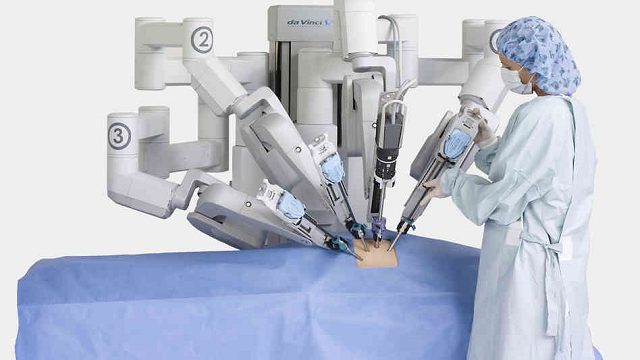
\includegraphics[width=1.1\pdfpagewidth]{da_vincy}%
%	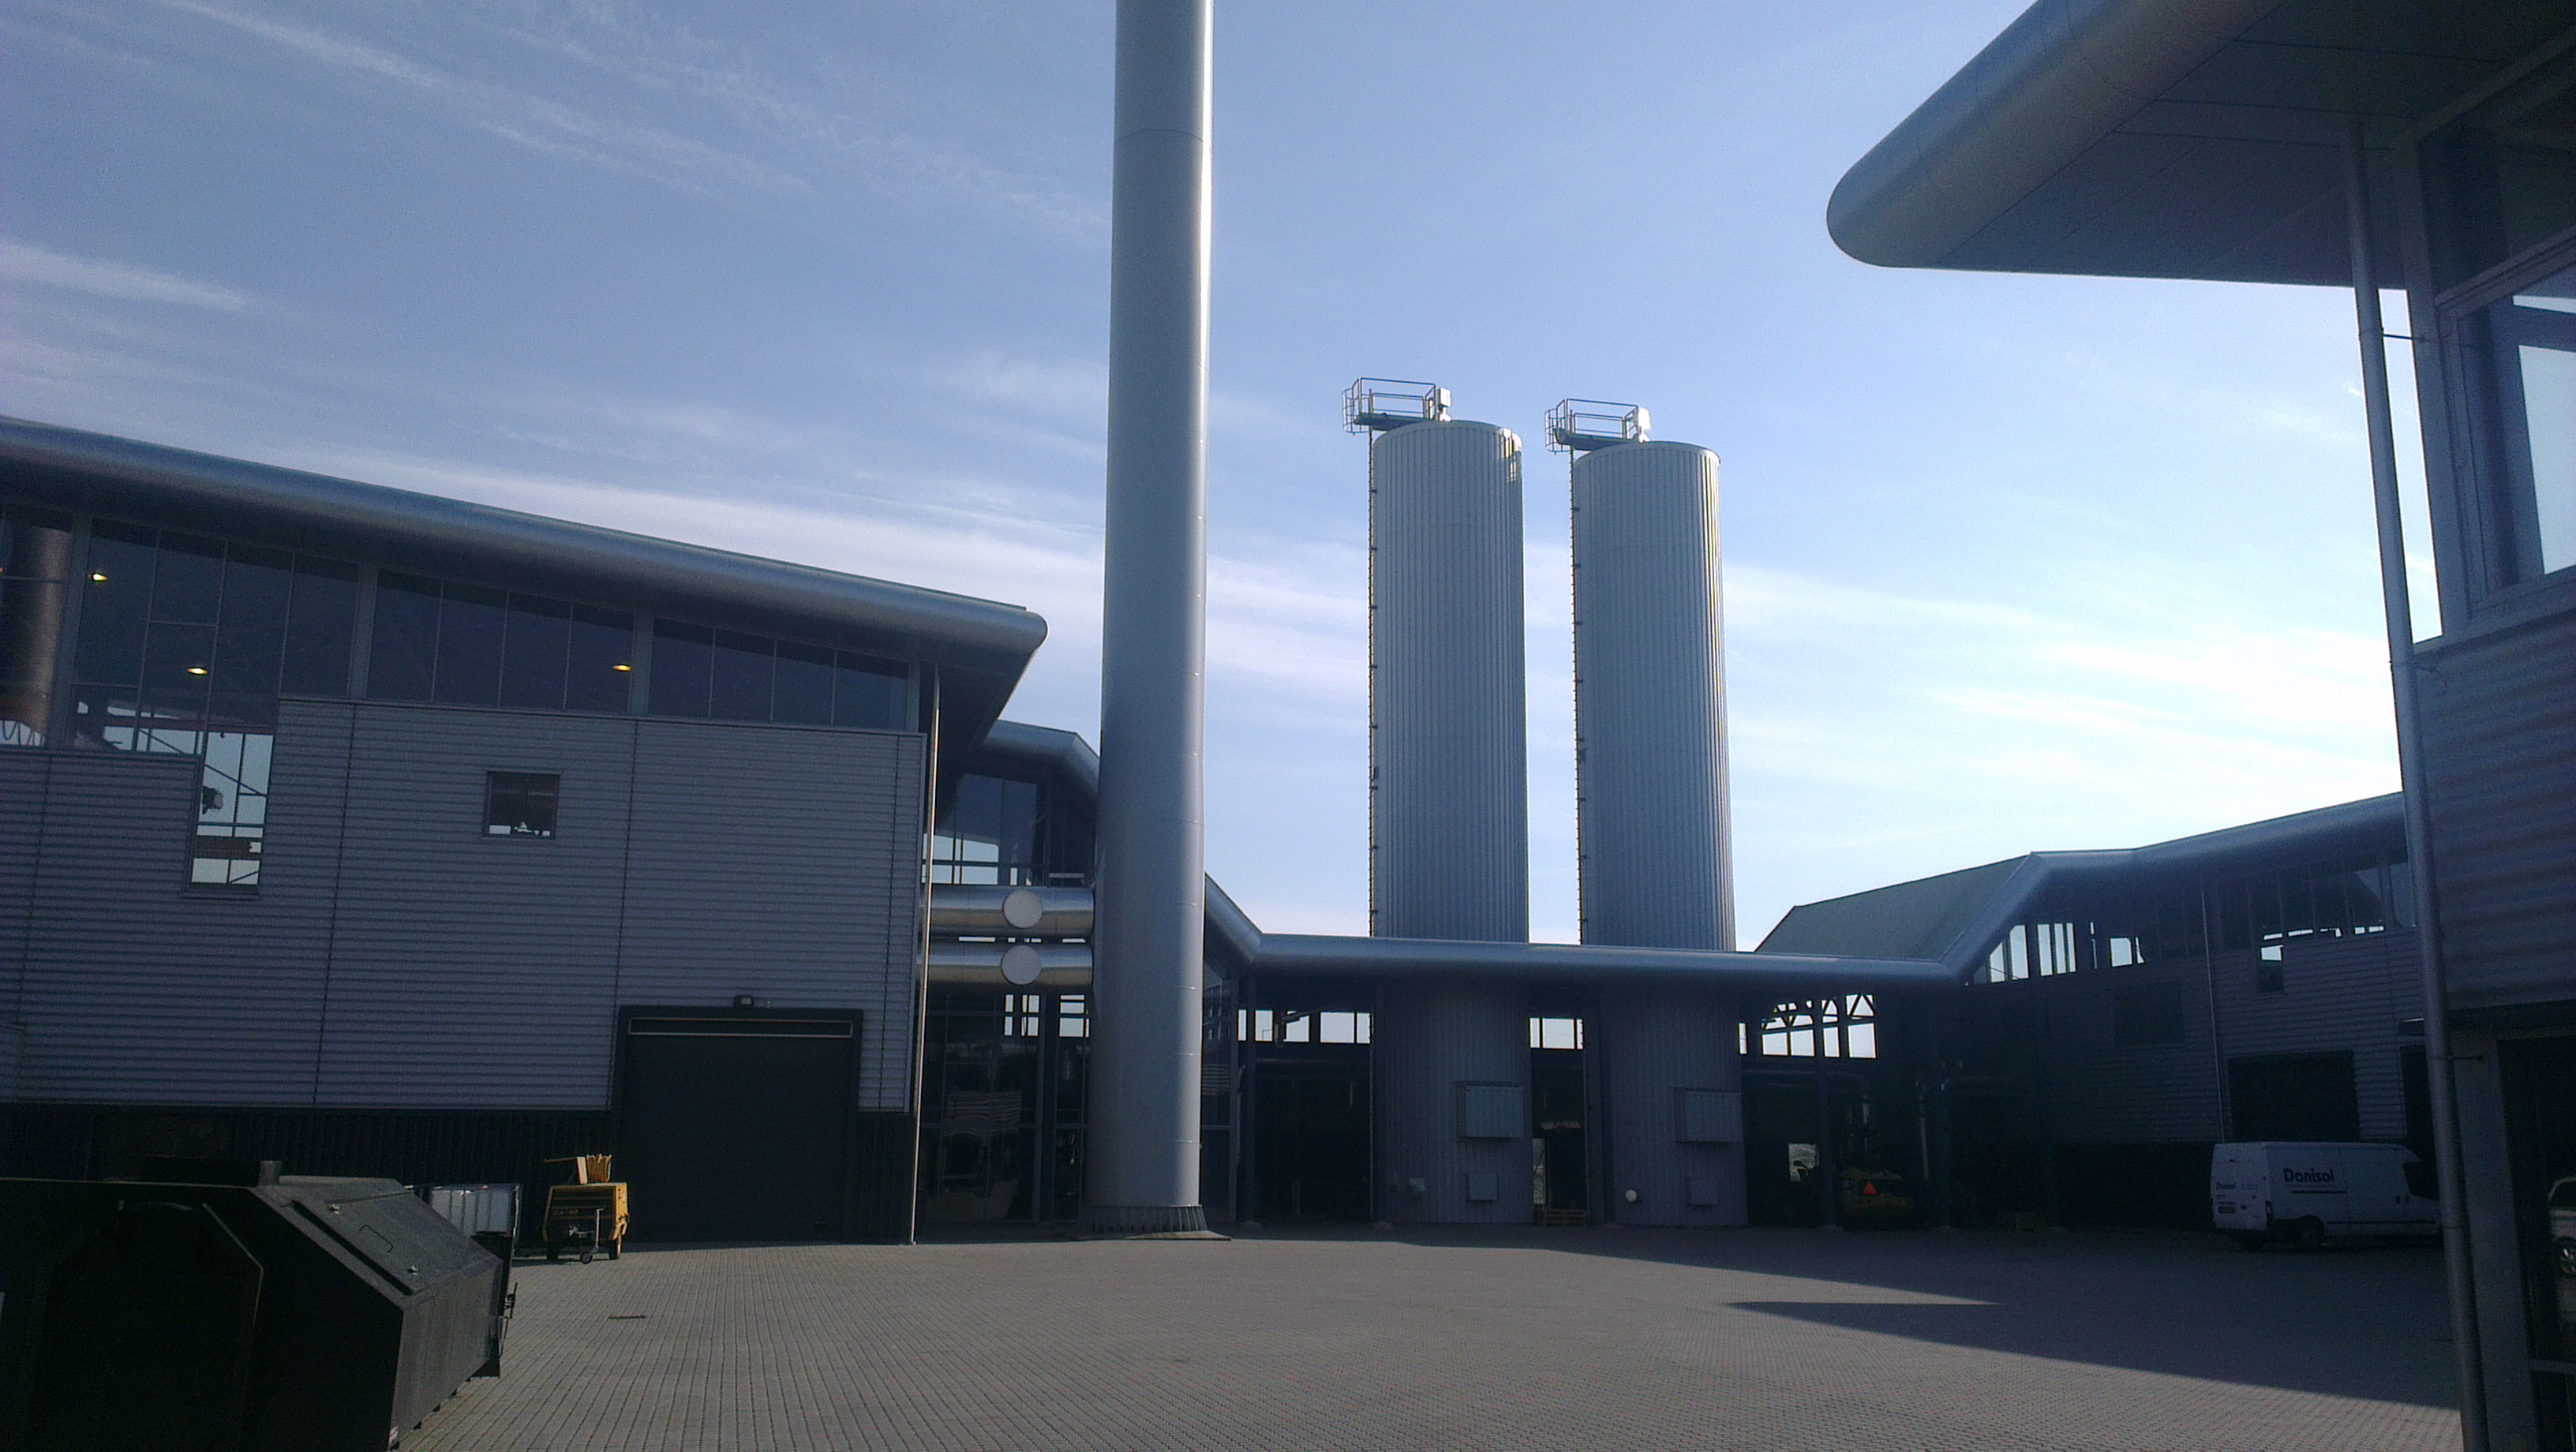
\includegraphics[width=0.45\pdfpagewidth]{formalia/2014-02-25 12.05.42.jpg}%	\caption{Virkningsgrad af den testede A/B hi-fi-forst�rker}
%\label{img_100wtest_linear}
\end{figure}
%\includepdf[scale=0.8,pages=1,pagecommand=\subsection{blub}]{testpdf}
%
\vspace{1cm}
\textsc{\Large \\
%Christian K�cks Lykkegaard \\
%s\\
%Economy track\\
%Elektronik \& IT\\
%Nordic Centre\\
%Fudan University\\
%September 27th 2012 \\
\textbf{School of Information and Communication Technology} \\
{\color{white}{..}}\\
Electronics \& IT\\
%s\\
Control and Automation \\
Final Thesis - CA4 Gr. 1032 \\
%Elektronik \& IT\\
Aalborg University\\
May 27$^\text{th}$ 2015\\
}\\
\end{titlepage}

\newpage
%\fchapter{}
\thispagestyle{empty}
%\begin{titlepage}
\vfil\null
\begin{center}
\bigskip \bigskip \bigskip
\vspace{1.0in}
\large
\bigskip \bigskip
\end{center} 
\normalsize
\vfil\null
\clearemptydoublepage
%\end{titlepage}

\thispagestyle{empty}
\begin{titlepage}


{\samepage 

\parbox{0.9\textwidth}{  
\raisebox{-15mm}{
\includegraphics[height=3.5cm]{AAU_LOGO_RGB_UK.png}}
\hfill{\footnotesize\noindent
\begin{tabular}{l}
            \textbf{School of Information and}\\
            \textbf{Communication Technology} \\
            Fredrik Bajers Vej 7 \\
            9220 Aalborg �st	\\
            Phone 99 40 86 00\\
            Fax 99 40 98 40\\
            http://www.es.aau.dk
\end{tabular}}}
\vspace{5mm}

    
\begin{tabular}{cc}
\parbox{7cm}{   
        {\bf Title:} Da Vinci Surgical Robot Automation \\        
        {\bf Master Thesis:} Control \& Automation\\              
        {\bf Project period:} Feb. $2^\text{nd} -$ June 3$^\text{rd}$ 2015\\
        {\bf Project group:} CA 15gr1032\\
        {\bf Participants:}\\
        \vspace{5mm}

\begin{minipage}[b]{0.7\linewidth}               	
     \underline{\phantom{JAERJAERJAERJAERoglidtmeretekst}}\\
      Britt Louise Jakobsen 
      
      \vspace{3mm}
	  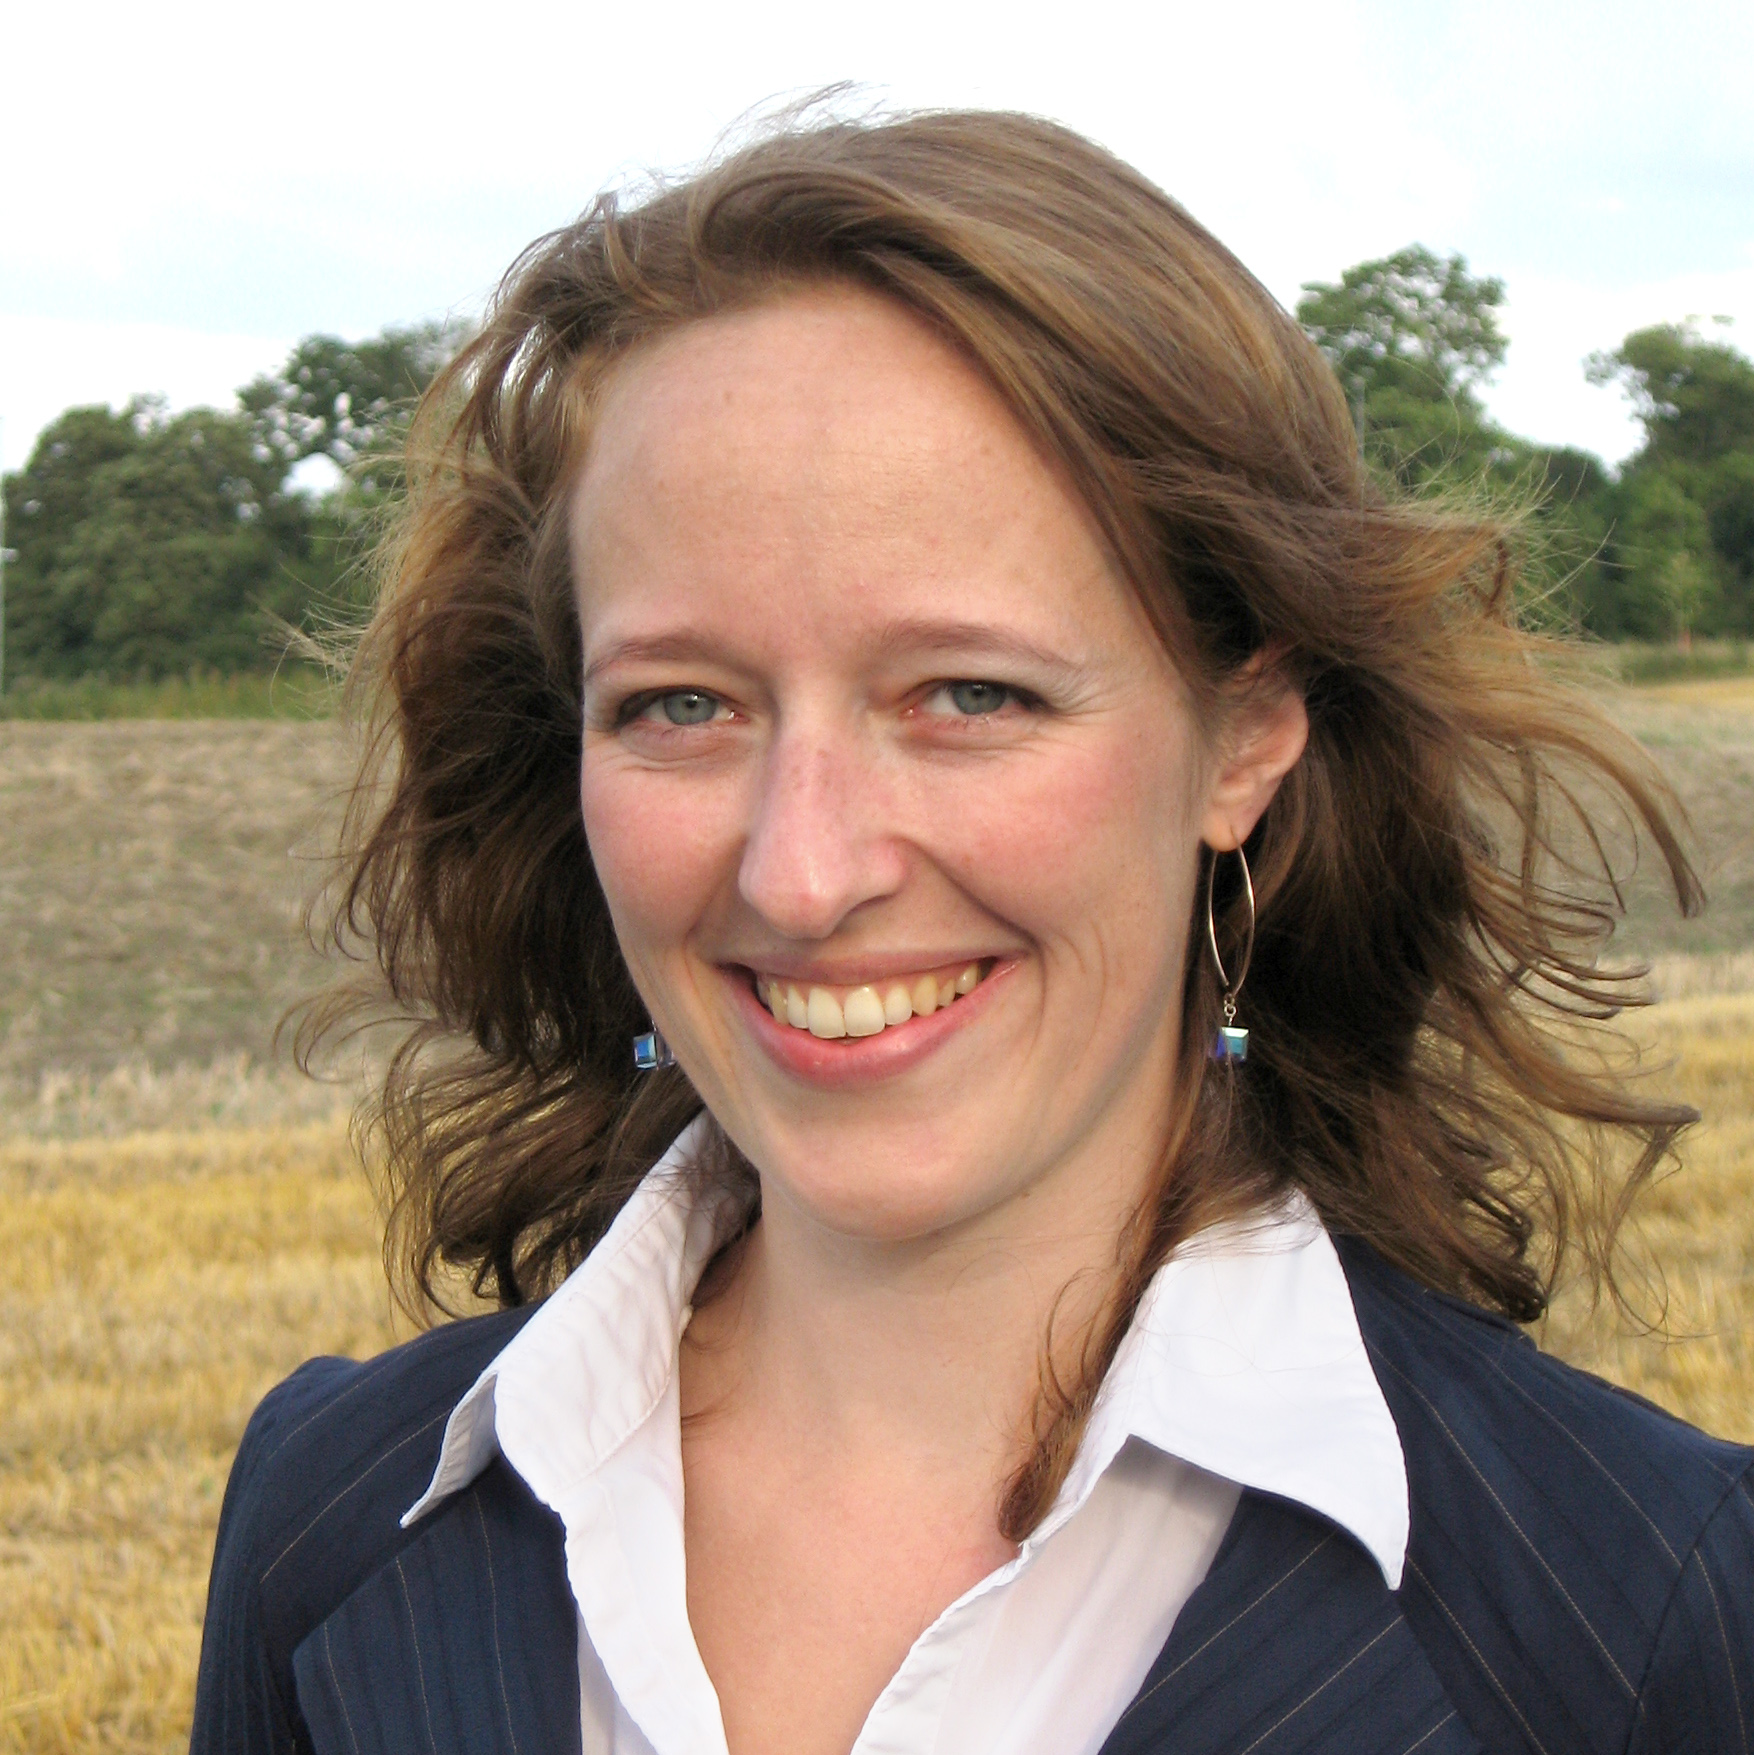
\includegraphics[width=0.52\textwidth]{IMG_3568_square.jpg}
\end{minipage}
  
\begin{minipage}[b]{0.7\linewidth}
   \vspace{10mm}
    \underline{\phantom{JAERJAERJAERJAERoglidtmeretekst}}\\
     Christian K{\o}cks Lykkegaard 

	\vspace{3mm}
	\includegraphics[width=0.52\textwidth]{IMG_3380.pdf}
\end{minipage}

\vspace{6mm}			
          
{\bf Supervisors:} \\
Prof. Rafa\l{} Wi\'{s}niewski\\
%Postdoc. Kasper Vinther\\
Ph.D. Tobias Leth\\
Assist. Prof. Christoffer Sloth\\
Postdoc. Karl Damkj�r Hansen\\  
               
        
{\bf Existing copies:} 5\\
{\bf Report:} \pageref{totalpage} pages \\
{\bf Appendix:} \pagedifference{appendixbegin}{appendixend} pages \\
\textbf{Attached:} 1 CD \\\\

\vfill } &
      
\parbox{7cm}{
\vspace{2mm}
\hfill 
\begin{tabular}{l}
      {\bf Abstract:}\bigskip \\
      \fbox{
      \parbox{7cm}{\bigskip
            {\vfill{\small In the course of the last few decades, robotic sur\-gery has become the  preferred type of operation within certain types of surgery, allowing the surgeon to perform precision procedures causing the patient a minimal amount of scarring while maintaining a exceptional overview of the operation site for the surgeon.


Advances are made within automation in the control of the robotic tools, providing the surgeon with more freedom and higher precision when performing operations. This thesis contributes to this advancement  through the use of barrier certificates with which safety of the automated control system can be guaranteed.


Control systems are developed for a number of use cases within robotic surgery for which safety  is certified through the construction of a barrier enclosing areas termed unsafe thus guaranteeing that the robotic tool will never cross this barrier. Two different approaches are taken: design of safety controllers based on manually constructed control barrier functions, and analytic verification of system safety using a software tool to construct the certificates.


The controllers are implemented on a first generation da Vinci surgical robot, and safety is verified for the developed control systems thus demonstrating the applicability of the theory of barrier certificates.


 \bigskip}}
      }\hspace{0.2em}}
\end{tabular}}

\end{tabular}

\vspace{-3mm}
\hspace{2mm}
\parbox{18cm}{
\noindent\footnotesize\textit{
\begin{flushleft} 
	The content of this report is freely available, but publication (with source reference) may only take place by agreement with the authors.	
\end{flushleft}}}
    
}
\end{titlepage}
\newpage
%\fchapter{}
\thispagestyle{empty}
%\begin{titlepage}
\vfil\null
\begin{center}
\bigskip \bigskip \bigskip
\vspace{1.0in}
\large
\bigskip \bigskip
\end{center} 
\normalsize
\vfil\null
\clearemptydoublepage
%\end{titlepage}

\setcounter{page}{1}
\renewcommand{\thepage}{\Roman{page}}

%\newgeometry{left=4.5cm,top=-0.5cm,bottom=2cm,textheight=28cm,includefoot,textwidth=16cm}
\chapter*{Preface}
\vspace*{-2mm}
This report documents the development process of a safe controller for automation of a surgical robot arm with patient safety guaranteed through barrier certificates. %, preventing the robot tool from entering predefined unsafe regions. 
The access to robot measurement data and opportunity to implement a controller heavily benefits from the previous work carried out on the da Vinci surgical robot in the Control Laboratory at Aalborg University.
The project is rated at 30 ECTS-points, and the work is conducted by the 4$^\text{th}$ semester group 1032 within the graduate program in Control and Automation at Aalborg University during the spring of 2015.


%The target group is supervisors, students and other interested parties at the School of Information and Communication Technology at the The Faculty of Engineering and Science.

\vspace*{-2mm}
\section*{Reading Guide}
\vspace*{-2mm}
The primary focus of this report is to design a controller and a barrier certificate, the certificate guaranteeing the safe control of a surgical robot, as an approach to draw closer to the possibility of implementing automated control tasks by surgical robots. 
%Controllers and certificates are designed for static as well as dynamic boundaries of unsafe regions, such as e.g. a beating heart.
After an introduction into surgical robotics and the definition of barrier certificates, two approaches to the design problem are described:
\vspace*{-3mm}
\begin{itemize}
\itemsep-1.4mm
\item Explicit approach: A barrier certificate is constructed and a safe controller is designed according to the method described in \citep{bib:org_control}.
\item Analytic approach: A controller is designed, criteria are constructed for a barrier certificate and  safety is verified by use of Putinar's Positivstellensatz.
%\item \autoref{part:closure} Discussion \textcolor{red}{REWRITE!!!}
\end{itemize}
\vspace*{-2mm}

Symbols, acronyms and a glossary are presented in the nomenclature before the main report.
A variant of the Harvard referencing is used for citations, with the author and publication year of the source given in square brackets, e.g. [Lasserre 78], and sources listed in the bibliography at the end of the main report. % contains all references used in the report. Books are indicated with author, title, publisher, year and ISBN. Web pages are indicated with author, title and year.
%Chapters in the main report are numerally numbered while appendices are alphabetically numbered.
A comprehensive appendix is included after the bibliography, containing introductions to the used software, detailed derivations, measurement logs and source code.
A digital copy of this report along with cited references, source code and simulation results can be found on the enclosed CD.

\vspace*{-2mm}
\section*{Acknowledgements}
\vspace*{-2mm}
The authors wish to thank Assistant Engineer Simon Jensen for a thorough introduction to the custom made AAU da Vinci hardware and design of a dynamic heart phantom platform; Ph.D. Tobias Leth for guidance in reference frame construction for robot kinematics;  Post Doc. Karl Damkj\ae r Hansen for an introduction to the AAU da Vinci robot operative system and help in implementing inverse kinematics; and Assistant Professor Christoffer Sloth for help and guidance with the theory behind barrier certificates and the use of SOSTOOLS.

Last but not least, it is desired to thank chief surgeon Johan Poulsen, robot assistant nurse Jane Petersson and surgeon Grazvydas Tuckus for sharing their insights in the use of surgical robotics and allowing the authors to attend a robotic surgery at Aalborg University Hospital.

%It is the wish of the authors to express a special appreciation to..

%\restoregeometry % efter denne side bruges de indstillinger der er sat i preamble
\newpage
%\fchapter{}
\thispagestyle{empty}
%\begin{titlepage}
\vfil\null
\begin{center}
\bigskip \bigskip \bigskip
\vspace{1.0in}
\large
\bigskip \bigskip
\end{center} 
\normalsize
\vfil\null
\clearemptydoublepage
%\end{titlepage}

\setlength\parskip{0ex}
\tableofcontents
\setlength\parskip{1ex}

\chapter*{Nomenclature}\label{chap:acronym}
\addcontentsline{toc}{chapter}{Nomenclature} % Adds chapter to TOC even though it is unnumbered
\printglossary[style=mcoltree,title=Glossary] %Print the glossary			%style=altlist
\printglossary[type=\acronymtype,style=glossary2col] %Print list of acronyms
\printglossary[type=symbols,style=altlong4col] %Print list of symbols
\clearpage

\section*{General Nomenclature Remarks}
\vspace{0.1cm}
\begin{itemize}
\item A dot above symbols indicate exclusively the time derivative, e.g. $\dot{x} = \dfrac{d}{dt}x(t)$
\item Well, maybe there is more
\item Or even more..
\end{itemize}

\textcolor{white}{\gls{analytic_func} \gls{rational_func} \gls{proper_func} \gls{injective_func} \gls{surjective_func} \gls{bijective_func} \gls{lipschitz} \gls{compact_space} \gls{hurwitz} \gls{dimension} \gls{extrinsic} \gls{intrinsic}}


\textcolor{red}{something simlar to this from \citep{bib:barrier_prajna}}
Notations: Most of the notations are standard. We denote
the set of real numbers by and the Euclidean n-space by $\mathbb{R}$.
The trace of an nxn matrix M, i.e., the sum of its diagonal elements,
is denoted by Tr(M). By f:X->Y we mean a function
mapping X subset Rn to Y subset Rm. We denote the spaces of
k-times continuously differentiable functions mapping
to Rm by Ck(X,Rm), and when m=1 we will write Ck(X).
Correspondingly, the spaces of continuous functions on are
denoted by C(X,Rn) and C(X). For a differentiable function
F:Rn->R, we use dF/dx(x) to denote the row vector
of partial derivatives of F with respect to x1,..xn. The Hessian
of a twice-differentiable function F:Rn->R is denoted
by d2F/dx2(x).

\cleardoublepage
\setcounter{page}{1}
\renewcommand{\thepage}{\arabic{page}}

\chapter{Introduction}\label{chap:intro}
In minimally invasive surgery (MIS), as opposed to traditional open surgery, only small incisions are made in the patient's abdomen or pelvis in order to gain access to the area under surgery, hence causing less trauma beyond this confined area. This in general provides the patient with quicker recovery, shorter hospital stay and less scarring.
One type of MIS is laparoscopy, invented in the beginning of the 20th century \citep{bib:laparoscopy}, where thin metal telescopes (laparoscopes) with specialized surgical tools attached are inserted into the patient through trocars, allowing the surgeon to maneuver the tools in the inflated abdomen guided by visual feedback from a flexible miniature camera (endoscope) inserted alongside the surgical tools \citep{bib:fascrs}.
In the 1980s robotic laparoscopic surgery was introduced as a master-slave system, where the surgeon controls a robot arm holding the surgical tools from a master console, instead of manipulating the instruments manually.

\section{Highlights in the Development of Surgical Robotics}
While the idea of roboticized telemedicine dates back to 1925 \citep{bib:telemed_predict}, the development of telesurgery was founded by NASA (National Aeronautics and Space Administration) in the 1970s \citep{bib:telesurg_history} combining research within virtual reality, robotics and medicine \citep{bib:brown_univ}, and the first robotic surgery procedure was accomplished in 1985 \citep{bib:telesurg_history}, followed by the first laparoscopic robotic surgical procedure in 1987 \citep{bib:brown_univ}.
The major research within telesurgery was funded by DARPA (Defence Advanced Research Project Administration, research administration under the U.S. Department of Defence) in the early 1990s, and two main teleoperation systems were developed from this research: da Vinci (from Intuitive Surgical) and Zeus (from Computer Motion) \citep{bib:telesurg_history}.

The first commercially available surgical robot ROBODOC (from Curexo) was introduced and performed the first robotic joint replacement surgery in 1992, and in 1994 the AESOP (from Computer Motion) was the first robotic system approved by the FDA (U.S. Food and Drug Administration) for general surgery \citep[p 74]{bib:telesurg_history,bib:surgical_book}.

In the early 1990s the U.S. Army developed MASH (Mobile Advanced Surgical Hospital) for loading and teleoperating wounded soldiers in vehicular operating rooms \citep{bib:brown_univ}, and in 1993 the idea for a robotic slave manipulator arm was conceived by Madhani after watching an episode of the tv-show M*A*S*H [SurgRob], and he created the Black Falcon during his work at MIT \citep{bib:black_falcon} later becoming he prototype of the da Vinci arms.

In 1996 the first tests were performed demonstrating the successful use of telementoring and telemanipulation of the endoscope by a surgeon placed several 100 m away from the operating room \citep{bib:telesurg_history}. 
In the late 1990s NASA and DARPA sponsored research within light-weight and deployable space surgical robotics for remote teleoperation, resulting in two main robotic systems: the Raven (from University of Washington) and M7 (from SRI International) [SurgRob].

In 1998 Zeus (from Computer Motion) was introduced and performed the first fully endoscopic robotic surgery and the initial beating-heart totally endoscopic coronary bypass procedure \citep{bib:brown_univ} and in 2000 da Vinci (from Intuitive Surgical) became the first robotic surgical system  to be approved by the FDA for general laparoscopic surgery \citep{bib:mddi}.

The first transatlantic telesurgical procedure, the Lindbergh Operation, was performed in 2001 by a team of French doctors in New York manipulating the arms of a Zeus robot to perform a gall bladder operation on a patient in Strasbourg \citep{bib:telesurg_history}. More research into remotely telementored and teleoperated robotic surgery was performed in the 2000s with the NEEMO (NASA Extreme Environment Mission Operations) projects in the Aquarius undersea lab in Florida, in 2003 with Zeus controlled from Ontario 2500 km away \citep[pp 75, 81]{bib:surgical_book} and in 2006 and 2007 with Raven and M7 controlled from Seattle \citep[pp 28, 82]{bib:surgical_book}. 

In 2005 DARPA launched the Trauma Pod program for developing an unmanned autonomous and semi-autonomous mobile military operation platform, funding research for e.g. SRI and for the Raven project. The goal of the first phase of the project was achieved in 2007 with the successful demonstration of a prototype trauma pod consisting of a da Vinci robot, a MASH stretcher and a custom nurse robot \citep[p 30]{bib:surgical_book}. The second phase aims at miniaturizing and integrating the systems \citep[p 31]{bib:surgical_book}, and in 2005 a demonstration was performed by roboticists, surgeons, aerospace engineers and networking experts in the desert placing the Raven patient manipulator and the controller console 100 m apart and relaying the communication link via a drone \citep{bib:docatadist}.

%In 2006 the first-ever demonstration of unmanned telesurgery with M7 [SurgRob]
%
%M7 performed the world's first automated ultrasound guided tumor biopsy in 2007 [SurgRob]
%
%2008 neuroArm was first used to remove a brain tumor [SurgRob]

NASA's first experiment in a zero gravity environment was performed with an acceleration compensated M7 in 2007 on a parabolic flight \citep[pp 29, 76, 85]{bib:surgical_book}, and in 2011 NASA sent the humanoid robot Robonaut 2 to ISS (International Space Station), and it has since been trained in telemedicine [SurgRob].







\section{State-of-the-Art in Surgical Robotics}
Most surgical robots used for telesurgery are master-slave systems which can be fully controlled by the surgeon \citep{bib:raven_debride}. The patient manipulator consists of 2-4 robotic arms, each having 6-7 degrees of freedom (DOF) \citep{bib:raven_debride} including the arm, wrist and the end-effector (the laparoscopic tool), one of the arms holding a stereo-vision endoscope. The end-effectors are positioned by high-precision motors and are able to reach spaces a human hand cannot \citep{bib:docatadist}.
Development is progressing within flexible end-effector tools \citep[p 74]{bib:surgical_book}, but even microrobots entering the body through natural orifices and controlled via electromagnetic fields or nanosensors and -actuators are being developed [SurgRob].

The 3D visual feedback from the endoscope is sent to the master console which can have eye-tracking for adaptive field of view and safety stop if the surgeon's gaze is not fixed at the operation site [SurgRob]. The control signals for the surgical instrument are generated with the controller joystick, which scales the surgeon's movements down to micro-movements \citep{bib:intuitive_monopoly} steerable through the (zoomed) 3D visual feedback. It also filters away tremor, and development is made within haptic feedback to the joystick \citep[p 89]{bib:surgical_book}, enhancing the surgeon's feel, enabling greater dexterity, accuracy and stability than a human hand.

In the first generations of surgical robotics the master and slave had to be in the same room (as is the case with da Vinci) \citep{bib:telesurg_history,bib:raven_debride,bib:surgical_book}. Experiments and development are made within minimizing and coping with delays for long-distance telesurgery and within miniaturization and robustness of the surgical robotic systems for use in harsh environments such as war and space, e.g. for da Vinci's potentially closest competitor, the open-source Raven.

Robotic surgical procedures are beginning to show superiority to conventional surgery for some procedures, but is still considerably more ecpensive \citep{bib:docatadist}. In some cases robotic procedures are faster than conventional surgeon procedures [SurgRob], but still in other it is much slower \citep{bib:raven_ii,bib:raven_debride}.
Autonomous procedures are still only implemented for entirely pre-planned motions of an operation, and depending on the type of operation not all subtasks in an operation are suited for autonomy \citep{bib:raven_debride,bib:raven_ii}.


\textcolor{red}{New generation: surgical care not only to soldiers but also to remote locations lacking specialized physicians. - better tactile feedback because the surgeon needs to feel the tissue and the difference in its stiffness}

Although the feasibility of conducting surgical interventions remotely has been demonstrated, there has not been market or clinical drivers strong enough to justify its implementation \citep[p 38]{bib:surgical_book}

\subsection{The da Vinci Surgical System}
Although several FDA approved robotic surgical systems exist, da Vinci is still the only commercially available system \citep{bib:docatadist,bib:intuitive_monopoly}. The first da Vinci prototype was developed at SRI under contract with the U.S. Army in the late 1980s [MDD], \citep{bib:brown_univ}, and in the early 1990s DARPA invested in the research \citep[p 74]{bib:surgical_book}. The the mid 1990s SRI licensed the manipulator design of Madhani along with many other patents, and in 1995 SRI founded Insuitive Surgical and the focus shifted from battlefield to commercial use in hospitals \citep{bib:intuitive_monopoly}.
In 1997 the first human trials were performed \citep{bib:intuitive_monopoly}, in 1999 the first market-ready da Vinci began tests [SurgRob] and the system was first approved by the FDA in 2000 \citep{bib:intuitive_monopoly,bib:brown_univ}. From 2000 until the merger in 2003 Intuitive Surgical and Computer Motion had a number of lengthy patent litigations \citep{bib:intuitive_monopoly,bib:telesurg_history}.

The da Vinci Surgical System still has the predominant market share with more than 3000 units installed worldwide due to being the first-mover in the field and due to their many patents \citep{bib:intuitive_monopoly}, and has only had one serious case of a patient dying after surgery (2002) [SurgRob].
The expiration of their patents in 2015 and 2016 \citep{bib:intuitive_monopoly} shows promise of many other robotic surgery systems entering the market, as both American, Canadian, European and not least Asian similar systems exist that are considerably cheaper than the da Vinci, and also more lightweight.

In 2013 Intuitive released the da Vinci Research Kit platform, built from mechanical components from first generation da Vinci (two arms and a surgeon console), open-source electronics and university-developed software \citep{bib:raven_observ}.

\subsection{The Raven Surgical Robot}
One potential challenger to da Vinci is the Raven \cite{bib:mddi}, an light-weight open-architecture 2-armed surgical robot \citep{bib:raven_debride,bib:raven_ii} originally developed by University of Washington funded by multiple U.S. government agencies including the Army and the Department of Defence (DoD) \citep[p 27]{bib:surgical_book}.
Raven-II is installed at 10 different universities in the U.S. and one in France \citep{bib:raven_ii}, sharing research innovations and using open-source software (including the ROS middleware) to create surgery subtasks \citep{bib:raven_debride}. 
As Intuitive Surgical's patents gradually expire the University of Washington is considering the possibility of spinning off the Raven into a start-up company \citep{bib:economist}.

The Raven robot is focused on remote telesurgery (with notable latency) in harsh conditions \citep{bib:docatadist}, and research at University of California has been made in teaching a computer model to autonomously mimic laparoscopic surgeons from recordings dynamic and kinematic data of their motions in a multi-state statistical Hidden Markov Model \citep{bib:economist}. 
The primary difficulty reported from controlling the Raven has been state estimation, necessary because of the uncertainty inherent in actuators and encoders connected to flexible elements via long cables \citep{bib:raven_debride} and the necessity of collision avoidance of the arms.



































\section{Focus of this Project}
Our focus:
safety
make forbidden areas where the robot cannot enter

ROS middleware layer as in Raven.
Prior work: designing planning and control algorithms for autonomous execution of several surgical subtasks (knot tying, suturing), advances in motion planning, control and perception: integrated task and motion planning ofhigh level task planning using state machines, and motion planning for low level planning algorithm  \citep{bib:raven_debride}
Raven-II inverse control process (not primarily to estimate the pose, in which case standard estimation methods like Kalman would be appropriate) is to calculate, give an desired true pose, the input pose to send the control sw to reach the desired true pose (detected pose with vision system assumed to be the true pose), estimate between measurements using updates from forward kinematics \citep{bib:raven_debride}.
da Vinci Research Kit: learning from demonstrations/by observation. Targets considered form convex regions spherical/linear. Patient Side Manipulators manipulates the instruments about a fixed point called the remote center of motion \citep{bib:raven_observ}.
DLR MIRo integrates torque sensing capabilities on the joint level, cosisting of actuation- position sensing- and torque sensing modules, can run in torque and impedance control mode. Virtual springs/potential fields are used to impose constraint forces preventing the robot from  entering predefined areas.


One should certainly take the risk of patient trauma when an automated surgery is conducted into account. This is seen in Therac-25. It is therefore a necessity to formally prove that the procedure is safe as seen in \citep{bib:safety}
\section{Technical Overview}
A simplified overview of the overall setup is provided in \autoref{fig:overview} as a block diagram. The setup is physically located at the department of Control and Automation at Aalborg University in the laboratory. The figure is structured with the highest abstraction layer at the top (i.e. the ROS (Robotic Operation System) - a software framework for robots [ROS artikkel]) environment which establish a wireless TCP/IP communication channel receiving all positions from the robot as feedback. It produces likewise positioning control signals to the NI (National Instruments) single board RIOs (Reconfigurable Input/Output) which handle all input/output communication with the user. The NI single board RIOs consist of a primary and a secondary board. The reason for having two RIO boards is solely the lack of input/outputs on one board.

The RIO boards direct the control signals to a cascaded controller taking in a velocity reference from the user and delivers a current control signal to the ESCON motor driver. The velocity and current controller are implemented in FPGA based hardware to ensure sufficient controller speed relative to the system \citep{bib:robot_paper}. The ESCON motor driver manage advanced processing and delivers essentially an appropriate PWM signal for the  actuators in form of seven maxon motors which represent the lowest abstraction layer located at the bottom of the figure.

The NI single board RIOs handle concurrently most safety precautions and enabling/disabling of the arm itself (see appendix ?? for location of the arm) through solenoids.
\begin{figure}[H]
	\center
	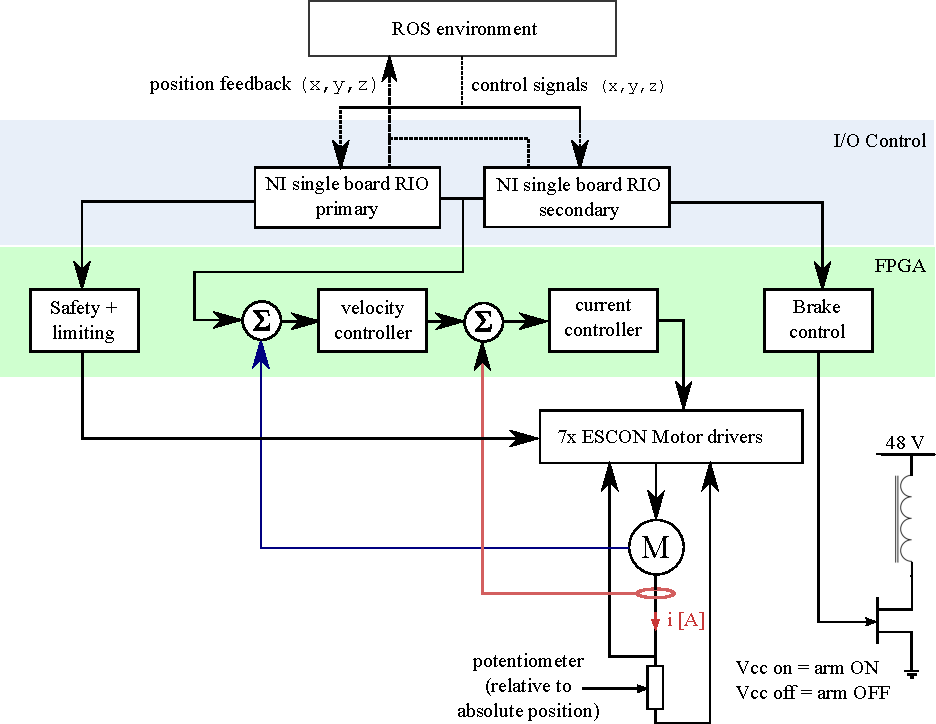
\includegraphics[width=0.95\textwidth]{overview.pdf}	\caption{This is a nice figure. Here illustrated for hand roll master.}
	\label{fig:overview}
\end{figure}
The focus of this thesis is the highest abstraction layer, i.e.the ROS environment. The purpose here primary constitute implementation of:
\begin{itemize}
\item Everything that require heavy processing \citep{bib:robot_paper}.
\item Non real-time processing or tasks with loose timing constraints \citep{bib:robot_paper}.
\end{itemize}
The above pool of stipulations will essentially and practically entail the follow main topics of this thesis:
\begin{itemize}
\item All user interaction
\item Positioning control loop
\item Path planning
\end{itemize}

\chapter{Safety Guarantee by Barrier Certificates}\label{chap:barrier_cerificates}
	A crucial matter when designing a controller for automated operation of robotic surgery tools is the necessity of guaranteed patient safety. The system has to not only be able to prevent the surgery tool from entering certain regions, e.g. penetrating the wall of the heart or cutting an artery, but to guarantee that this cannot happen under any circumstances.


Casting the controller design problem as an optimization problem with constraints, such as \gls{mpc}, could in principle guarantee that the tool would not enter a predefined area. Indeed, \gls{mpc} is a method which is very popular at the higher abstraction layers, such as setpoint control \citep{bib:mpc_simon} which is the case in this specific study. However, most solvers such as the Matlab plugin \texttt{cvx} requires convexity in the performance function and its constraints to be able to find a global minimum. This will at best be a lucky special case that unsafe regions can be defined through a convex function.  
Furthermore, \gls{mpc} is mostly used in systems with slow dynamics, i.e. dynamics where the time constant is measured in seconds or even minutes \citep{bib:mpc_slow}. This is obviously due to heavy online computations and numerous iterations. Systems containing these time constants are usually thermal systems and not mechanical systems. Additionally, the feasibility of the optimization problem is not very transparent and it is well known that \texttt{cvx} is very likely to crash due to infeasibility.
%, but a hard constraint would fail to follow the dynamics of a moving area boundary such as a beating heart. 

Another very elegant and computationally efficient approach to the safe controller analysis and design problem is the use of barrier certificates, which provide a formal proof of safe operation in infinite time horizon \citep{bib:prajna_framework,bib:safety}. This chapter describes the requirements for the construction of barrier certificates along with notation used in relation to these.
%


%dealing with those topics within robotic surgeries feature necessary conditions to guarantee the patient safety and to avert patient trauma .



\section{Constraints for a Barrier Certificate}\label{sec:safety-def}

When a barrier certificate can be found for a (closed-loop) dynamical system, the controller is guaranteed to be safe. In the following the notion of safety is defined in order to describe the guarantee extent of a barrier certificate. A general state-space representation of an $n$-dimensional non-linear system is considered:
\begin{equation}
\dot{\mathbf{x}} = f_{cl}(\mathbf{x}) + h(\mathbf{x})\,\mathbf{d} = f(\mathbf{x}) + g(\mathbf{x})\,\mathbf{u} + h(\mathbf{x})\,\mathbf{d}
\label{eq:general_statespace}
\end{equation}
\begin{tabular}{rl} 
where &  \\
\gls{x} &  is the state, $\mathbf{x}(t) \in \mathbb{R}^n$\\
\gls{u} & is the control input, $\mathbf{u}(t) \in \mathbb{R}^m$\\
\gls{d} & is the disturbance input, $\mathbf{d}(t) \in D \subseteq \mathbb{R}^p$ \\
\gls{f} & is a non-linear function, $f:\mathbb{R}^n \rightarrow \mathbb{R}^n$\\
\gls{g} & is a non-linear function, $g:\mathbb{R}^n \rightarrow \mathbb{R}^{n \times m}$\\
\gls{h} & is a non-linear function, $h:\mathbb{R}^n \rightarrow \mathbb{R}^{n \times p}$
\end{tabular}\\

Consider a subspace of the state-space $\mathcal{X}\subseteq\mathbb{R}^n$ defining e.g. the physically feasible states for the system in \autoref{eq:general_statespace}. Within this region $\mathcal{X}$, define the two non-intersecting subspaces $\mathcal{X}_u\subset\mathcal{X}$ and $\mathcal{X}_0\subseteq\mathcal{X}$, defining an unsafe  and a safe region, respectively. The unsafe region contains the states which the trajectory of the system must never enter, e.g. for a surgical robot this space could be the collection of veins and organs near the operation site, for which perforation is prohibited. The safe region contains all the states which the trajectory of the system is allowed to and may be required to enter, e.g. the operation site and a region for entering the area in the abdomen.
Now safety of a closed-loop control system is given according to \citep{bib:safety,bib:prajna_framework} as:
%\begin{exa}

\begin{defn}[Safety of a System]\label{def:safety}
Denote a trajectory starting in $x(0)=x_0$ and with bounded disturbance function $\bar{d}:\mathbb{R}_{\geq 0}\rightarrow D$ by $\phi_{x_0}^{\bar{d}}$, defined by 
\begin{equation}
\frac{d \phi_{x_0}^{\bar{d}} }{dt} = f_{cl}\left( \phi_{x_0}^{\bar{d}} (t) \right) + h\left( \phi_{x_0}^{\bar{d}} (t) \right) \bar{d}(t)
\end{equation}
The system $\Gamma_{cl} = (f_{cl},h,\mathcal{X},\mathcal{X}_0,\mathcal{X}_u,D)$ is unsafe if there exists a $t \in [0,$\gls{T}$]$ such that the trajectory $\phi_{\mathcal{X}_0}^{\bar{d}}:\,[0,T]\rightarrow \mathbb{R}^n$ with initial state $x_0\in \mathcal{X}_0$ and bounded disturbance function $\bar{d}$ satisfies
\begin{flalign}
\left( \phi_{\mathcal{X}_0}^{\bar{d}}([0,t]) \cap \mathcal{X}_u \right) \neq \emptyset \kk \text{and} \kk 
\phi_{\mathcal{X}_0}^{\bar{d}}([0,t]) \subseteq \mathcal{X}
\label{eq:defsafety}
\end{flalign}
\noindent
The system $\Gamma_{cl}$ is safe if there are no unsafe trajectories.
\end{defn}

%\vspace{-0.2cm}
%
%\begin{longtable}{p{.9\textwidth} p{.1\textwidth} p{.1\textwidth}} 
%Where  & & \\
%\gls{fcl} is a potential non-linear function with the closed loop characteristic:\\ \kk $f_\text{cl}: x \mapsto f(x)+g(x)k(x)$ where \gls{k} is the feedback gain with the map $k: \mathbb{R}^n \rightarrow \mathbb{R}^m$ & [$\cdot$] &  \\
%\gls{X} is the set of all allowed states & [$\cdot$] &  \\
%\gls{X0} is the set of all allowed initial states & [$\cdot$] &  \\
%\gls{Xu} is the set of all unsafe states & [$\cdot$] &  \\
%\gls{phi} is the set of all allowed initial conditions with the bounded disturbance input \gls{dbar} & [$\cdot$]
%\end{longtable}

A graphical interpretation of \autoref{eq:defsafety} is shown in \autoref{fig:defsafety}.

\begin{figure}[H]
	\center
	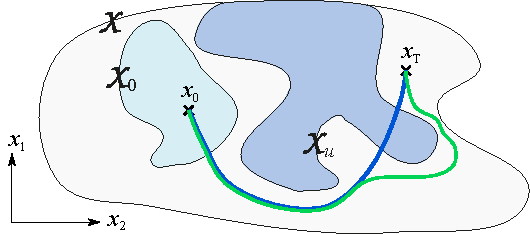
\includegraphics[width=0.6\textwidth]{safety.pdf}	
	\caption{Graphical interpretation of \autoref{eq:defsafety} in the state space. The blue trajectory is unsafe because $\left( \phi_{\mathcal{X}_0}^{\bar{d}}([0,t]) \cap \mathcal{X}_u \right) \neq \emptyset$, while the green trajectory is safe.}
	\label{fig:defsafety}
\end{figure}
%\end{exa}

Disturbances are not considered in the scope of this project, and hence $\mathbf{d}\in D$ is considered to be zero in the remainder of this thesis.

For the system in \autoref{eq:general_statespace} safety can be guaranteed if a barrier certificate for the system exists. A barrier certificate is defined as a function of the system state, satisfying a set of inequalities, entailing that its zero level set in the state space forms a barrier between the safe set of initial states $\mathcal{X}_0$ and the unsafe set $\mathcal{X}_u$, thereby certifying system safety \citep{bib:prajna_framework}.


If a barrier certificate can be defined, safety can be guaranteed for the closed-loop system in the region $\mathcal{X}$, with unsafe region $\mathcal{X}_u$, defined by positive values of the barrier function, and (safe) initial region $\mathcal{X}_0$, defined by non-positive values of the barrier function. In the below the notation $L_{f_{cl}}B(\mathbf{x})$ denotes the Lie derivative of \gls{bar} along the vector field of the closed-loop system $f_{cl}(\mathbf{x})$, corresponding to the time derivative of the barrier function i.e.
\begin{equation}
L_{f_{cl}}B(\mathbf{x})=\frac{dB(\mathbf{x})}{d\mathbf{x}}f_{cl}(\mathbf{x})=\frac{dB(\mathbf{x})}{d\mathbf{x}}\frac{d\mathbf{x}(t)}{dt}=\frac{dB(\mathbf{x}(t))}{dt}
\end{equation}

Requiring that the time derivative of the barrier function must be nonpositive on the entire set $\mathcal{X}$ (see \autoref{def:barrier_certificate}) corresponds to the value of the barrier function decreasing over time, hence seeking the minimum of the (convex) barrier certificate. Requiring the trajectory of the state to start within the safe set $\mathcal{X}_0$ this means that the trajectory will never cross the zero level set and enter the unsafe set $\mathcal{X}_u$, as this set only contains values of the barrier function larger than the initial value.

\begin{defn}[Barrier Certificate]\label{def:barrier_certificate}	
If a barrier certificate can be constructed as a continuous and differentiable function $B(\mathbf{x}):\mathcal{X} \rightarrow \mathbb{R}$ adhering to the following inequalities  \citep{bib:prajna_framework}:
\begin{subequations}\label{eq:barrier_constraints}
\begin{flalign}
B(\mathbf{x}) &\leq 0 \kk  \forall \hspace{2mm} \mathbf{x} \in \mathcal{X}_0  \label{cer1}\\
B(\mathbf{x}) &> 0  \kk  \forall \hspace{2mm} \mathbf{x} \in \mathcal{X}_u \label{cer2} \\
L_{f_{cl}}B(\mathbf{x}) &\leq 0 \kk  \forall \hspace{2mm} \mathbf{x} \in \mathcal{X} \label{cer3}
\end{flalign}
\end{subequations}
Then safety of the closed-loop system $f_{cl}(\mathbf{x})$, as defined in \autoref{def:safety}, is guaranteed. 
\end{defn}


From \autoref{eq:barrier_constraints} it can be seen that the function $B(\mathbf{x})$ must be constructed such that its zero level set delimits and separates the safe and the unsafe regions, while the Lie derivative constraint imposes that the derivative $dB(\mathbf{x})/d\mathbf{x}$ must have the opposite sign of the state derivative $d\mathbf{x}/dt$ for any state within the region $\mathcal{X}$, where $B(\mathbf{x})$ is defined. 
Note how according to \autoref{cer3} the barrier certificate requires mere stability and not asymptotic stability ($L_{f_{cl}}B(\mathbf{x})<0$) of the system trajectory. This is rarely enough when dealing with physical systems, however, mathematically it is sufficient.

Furthermore from \autoref{cer3} it is deduced that a controller incorporating the barrier certificate in its design will ensure stability if $B(\mathbf{x})$ has a finite minimum value. This entails that $B(\mathbf{x}) $ is radially unbounded if $\mathcal{X}$ encompasses the entire state-space:
\begin{equation}
\underset{\mathbf{x}\rightarrow \pm\infty}{\lim} B(\mathbf{x})= \infty \kk \text{if} \kk \mathcal{X}=\mathbb{R}^n
\end{equation}

\subsubsection{Nexus to Lyapunov Functions}
\vspace*{-3mm}
As it can be seen from \autoref{eq:barrier_constraints} the definition of a barrier certificate strongly resembles that of a Lyapunov function, and indeed the Lie derivative nonpositivity constraint is identical to the time derivative constraint to a Lyapunov function $V(\mathbf{x})$, a Lyapunov candidate function for a stable system given by
\vspace*{-5mm}
%\begin{equation}
%\dot{x}  = f(x) = \frac{d x}{d t} \qquad
%\left\{ \begin{array}{r l l}
%L_fB(x) \hspace*{-2mm}&= \tfrac{d B(x)}{d x} f(x) \hspace*{-2mm}&= \tfrac{d B(x)}{d x} \frac{d x}{d t}\\
%\dot{V}(x) \hspace*{-2mm}&= \tfrac{d V(x)}{d t} \hspace*{-2mm}&= \tfrac{d V(x)}{d x}\tfrac{d x}{d t}
%\end{array} \right. \label{eq:dBdt_dVdt}
%\end{equation}
\begin{subequations}\label{eq:lyap}
\begin{align}
V(\mathbf{x}) &> 0 \kk \forall \hspace{2mm}\mathbf{x} \in \mathbb{R}\setminus\{0\}\\
\dot{V}(\mathbf{x}) &\leq 0 \kk \forall \hspace{2mm}\mathbf{x} \in \mathbb{R} \label{eq:lyap_stable}
\end{align}	
and for a system with an asymptotically stable equilibrium in $\mathbf{x}=0$, \autoref{eq:lyap_stable} is replaced by
\vspace*{-2mm}
\begin{equation}
\dot{V}(\mathbf{x}) < 0 \kk \forall \hspace{2mm}\mathbf{x} \in \mathbb{R}\setminus\{0\}\label{eq:lyap_vdot_minus_criticalpoint}
\end{equation}
\end{subequations}
As such a barrier certificate can be seen as an offset Lyapunov function with negative values in the safe region. The stable focus may also be offset from $\mathbf{x}=0$. However, a barrier function may also take other (non-convex) forms. 



\section{Approaches to the Problem of Guaranteeing System Safety}
Two approaches to the problem of guaranteeing safety of a system through the construction of barrier certificates are used in the following: design of safe controllers and safety verification of control systems.

In \autoref{chap:cbf} a method of designing guaranteed safe controllers from barrier certificates is described, based on \citep{bib:org_control}. This method is used in chapters \ref{chap:cbf_1d_static} through \ref{chap:cbf_3d_static}, where barrier certificates are constructed by hand, and guaranteed safe controllers are designed and implemented on the da Vinci surgical robot. The safe controller is used in combination with a linear state space controller designed through pole placement for setpoint control in the safe region. In \autoref{chap:cbf_1d_static} and \ref{chap:cbf_1d_dynamic} system models of different orders are considered in 1D Cartesian space, with static and dynamic boundaries (zero level sets) of the barrier function, respectively, while in \autoref{chap:cbf_3d_static} a system model is considered in 3D Cartesian space. 

In \autoref{chap:putinar} a recasting of \autoref{def:barrier_certificate}  according to \citep{bib:sos_putinar_lasserre} is presented, allowing for automated construction of barrier certificates with an existing software toolbox for MATLAB. 
When a barrier certificate can be found using this toolbox, system safety is hereby certified.
In \autoref{chap:sostools} this method of safety verification is applied to linear position-control systems corresponding to the linear state space controllers presented in \autoref{chap:cbf_1d_static}.
%Similarly to \autoref{part:cbf} the following chapters verify controller safety for system models of different orders in 1D and 3D space, with static and dynamic boundaries (zero level sets) of the barrier function.
%\autoref{chap:sos_1d_static} \autoref{chap:sos_1d_dynamic} \autoref{chap:sos_3d_static} \autoref{chap:sos_3d_dynamic}



%The design of a safe controller features the property that a supplied control signal ensures compliance of the definition described in \autoref{sec:safety-def}.









%\part[Safe Controller Design from Control Barrier Functions]{Safe Controller Design from \\Control Barrier Functions}\chaptermark{Safe Controller Design from Control Barrier Functions}\label{part:cbf}
\chapter{Controller Design from CBFs}\label{chap:cbf}
	\glsreset{clf}\glsreset{cbf}
Based on \citep{bib:artstein}, which founded \gls{clf}s, a \gls{cbf} can be created \citep{bib:org_control}. With a system $\dot{x}=f(x)+g(x)u$, a \gls{cbf} exist if the below constraints are fulfilled:
\begin{flalign}
& x\in \mathcal{X}_u \hspace{0.3cm} \Rightarrow \hspace{0.3cm} B(x) > 0  \label{req1} \\
& L_gB(x) = 0 \hspace{0.3cm} \Rightarrow \hspace{0.3cm} L_fB(x) < 0 \label{req2} \\
& \{ x \in \mathcal{X} | B(x) \leq 0 \} \neq \emptyset \label{req3}
\end{flalign}
\vspace{-0.8cm}
\begin{longtable}{p{.9\textwidth} p{.1\textwidth} p{.1\textwidth}} 
Where  & & \\
$L_f(x)$ is the Lie derivative of $B(x)$ along the vector field  $f(x)$, i.e. $\frac{\partial B(x)}{\partial x}f(x)$ & [$\cdot$] \\ 
$L_f(x)$ is the Lie derivative of $B(x)$ along the vector field  $g(x)$, i.e. $\frac{\partial B(x)}{\partial x}g(x)$ & [$\cdot$] 
\end{longtable}
\vspace*{-0.2cm}
Taking a look at \autoref{req1} it states essentially the same as \autoref{cer2}, i.e. the unsafe area exist whenever $B(x)>0$. This makes it possible to design an unsafe region. \Autoref{req2} put forth the requirement that the gradient along the vector field $f(x)$ must point away from the barrier extremities whenever the input is with no significance (except for the critical point). \Autoref{req3} simply states that the safe area must contain some states as control otherwise is impossible.
\section{Safe Controller for Instrument Slide}
The slide movement is visualized in \autoref{fig:slidefig} and an overview of terms used in this section is found in \autoref{fig:safe:overview}.
\begin{figure}[H]
    \centering
    \begin{minipage}{.5\textwidth}
        \centering
        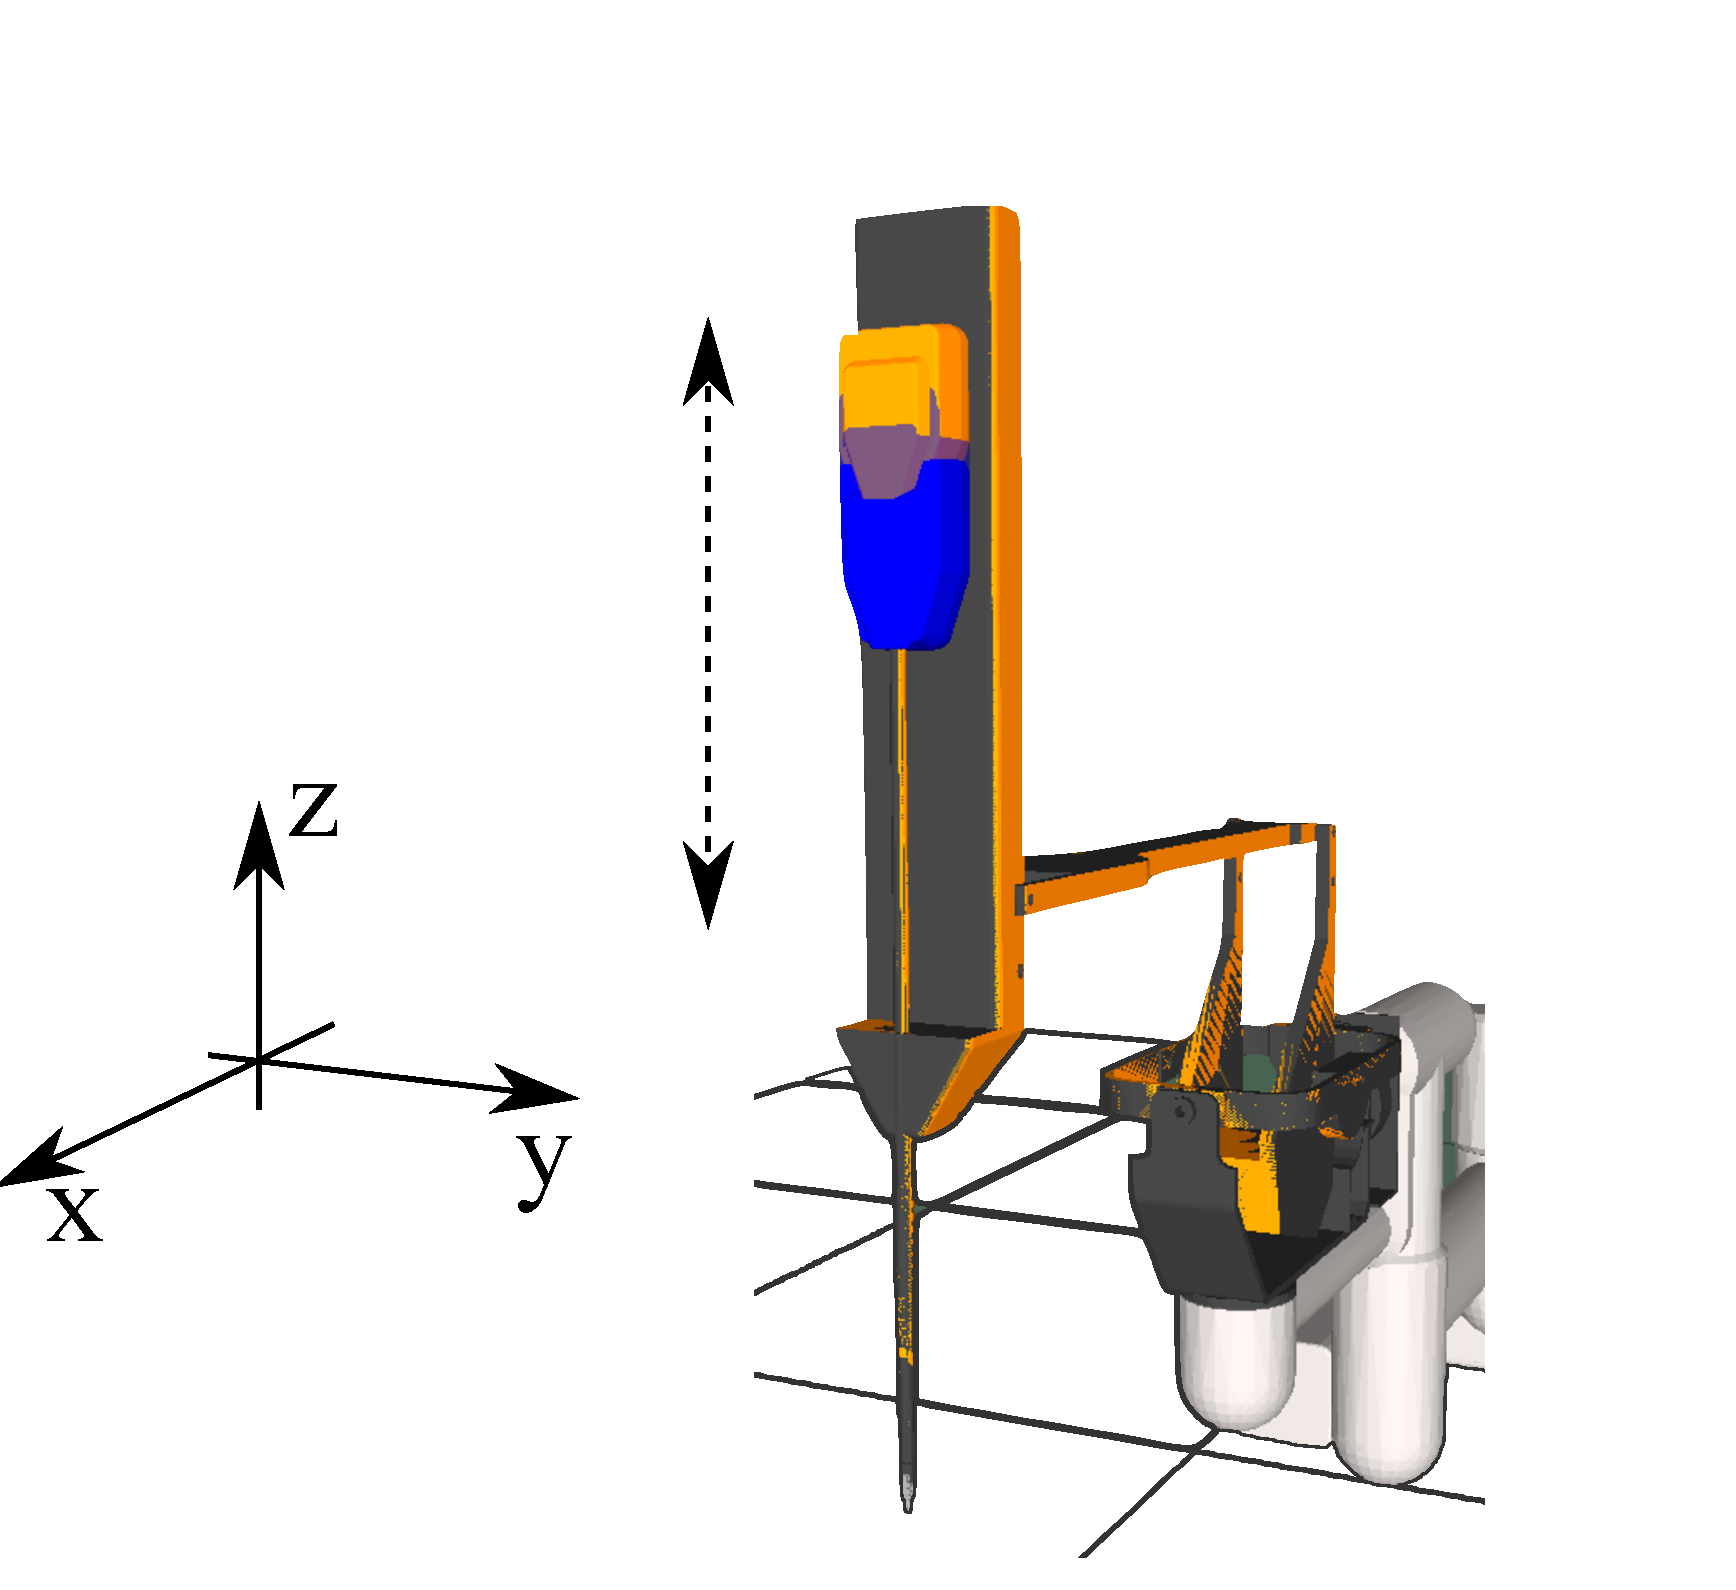
\includegraphics[width=0.73\linewidth]{slidemovefigure.pdf}
        \caption{Illustration of slide movement.}
        \label{fig:slidefig}
    \end{minipage}%
    \begin{minipage}{0.5\textwidth}
        \centering
        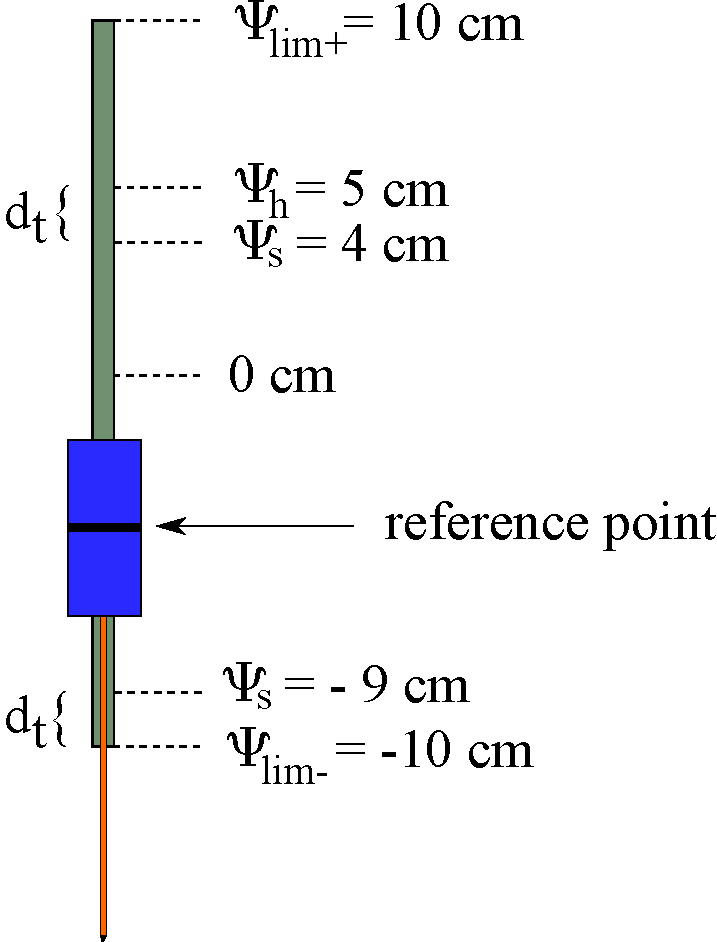
\includegraphics[width=0.7\linewidth]{slide_overview.pdf}
        \caption{Boundaries used in this section.}
        \label{fig:safe:overview}
    \end{minipage}
\end{figure}
A system model is required before any controller design may be initiated.
%\hspace{1cm }\texttt{rostopic echo joint\_states/position[6]} \hspace{0.2cm} {\color{blue}{\# Be sure to have the ROS environment correctly configured according to \autoref{app:ros}}}
\section{Modelling of Slide Movement}
 To obtain a model, a step response will be performed on the slide movement. The slide position can be measured by subscribing to the \texttt{joint\_state} topic in \gls{ros}. The experiment is described in further details in \autoref{app:meas}. To model the system, a step is added to the system. The step response is plotted in \autoref{fig:stepresponseslide}.
\begin{figure}[H]
\center
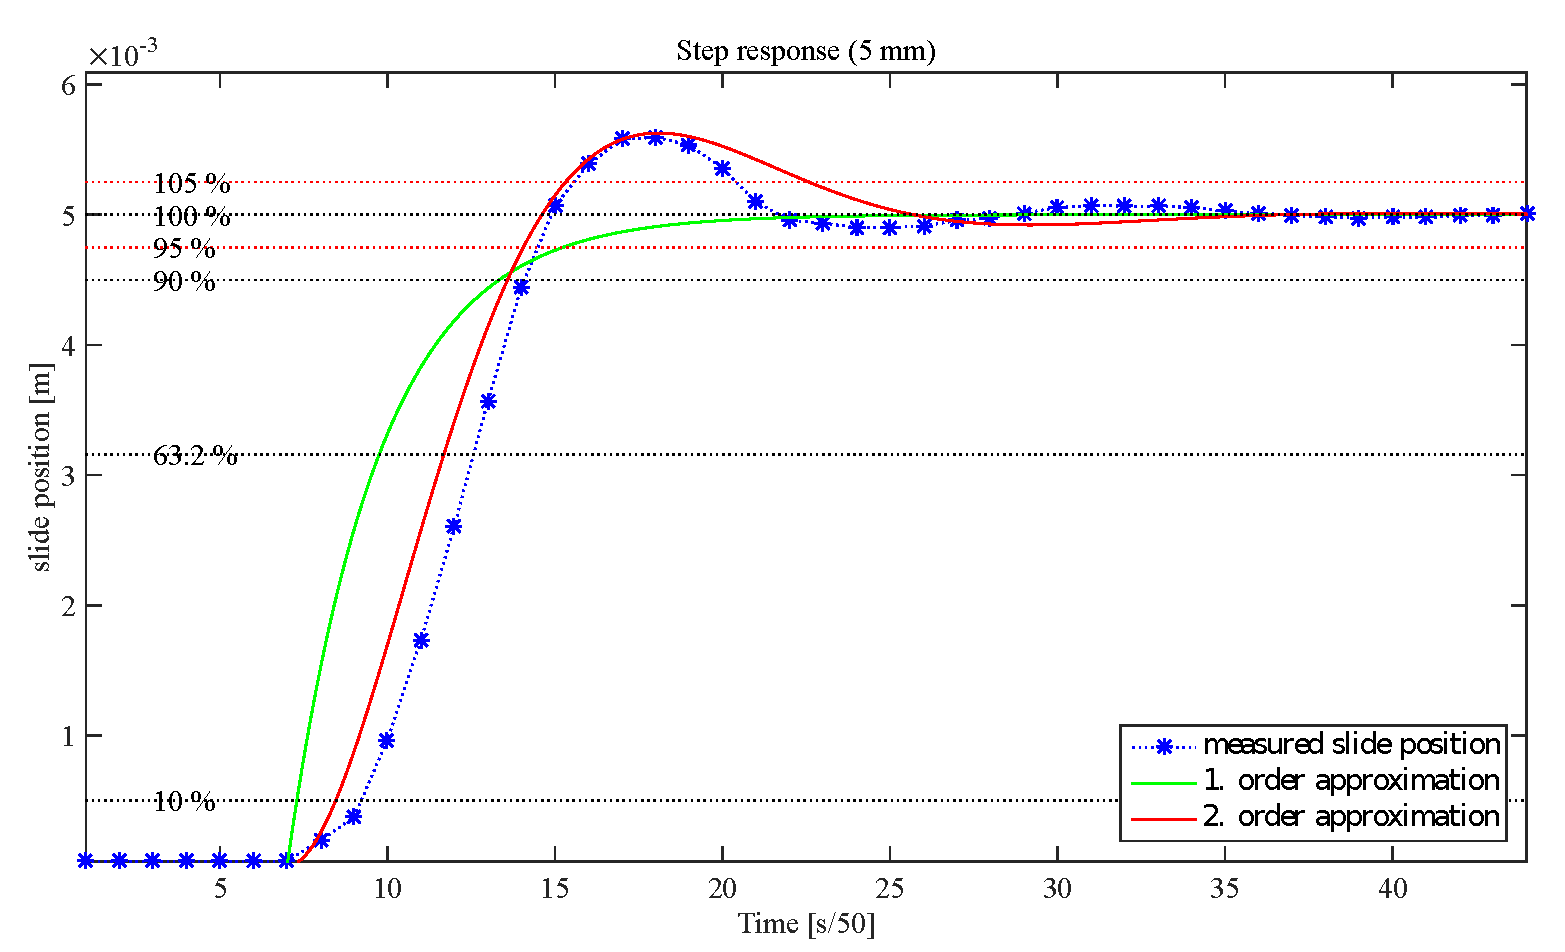
\includegraphics[scale=0.5]{step_slide.pdf}
\caption{Step response from 0\,mm to 5\,mm. Plot details and measurements can be found in \autoref{app:cd} as \texttt{matlab\_scripts/slide\_step/plot\_slide\_pos.m}}
\label{fig:stepresponseslide}
\end{figure}
It is clear that this could be well approximated with an underdamped second order model (complex roots), however for initial simplicity and because modelling is not a focus point in this thesis, merely a simple model of the slide movement is used (it shall later be approximated to a second order model). Therefore, with some good will, it is approximated to a linear first order system with a dominating time constant \gls{taus}: 
\begin{flalign*}
& Y(s) = \dfrac{1}{\tau_s s + 1}U(s) =  \dfrac{1/\tau_s}{s + 1/\tau_s}\,U(s) = (s+1/\tau_s)^{-1}\,1/\tau_s\,U(s) \kk  \overset{\overset{Y(s)=(C(sI-A)^{-1}B+D)U(s)}{\longrightarrow}}{\scriptsize \text{compare to obtain SS form}}  \\ 
& \dot{x} = \underbrace{-\tau_s^{-1}\,x}_{f_s(x)} + \underbrace{\tau_s^{-1}}_{g_s(x)} u
\end{flalign*}
Thus the system matrix $A$ and the input matrix $B$ can be seen easily. For the sake of generalization, they are named $f_s$ and $g_s$, i.e.:
\begin{flalign*}
f_s(x) = -\tau^{-1}x \kk \wedge \kk g_s(x) = \tau_s^{-1}
\end{flalign*}
A suitable time constant $\tau_s$ can be read from \autoref{fig:stepresponseslide} to:
\begin{flalign*}
\tau_s = 55\, \text{ms}
\end{flalign*} 
\section{Construction of CBF}
To illustrate the usefulness of \gls{cbf}s, a palpable example hereof will be created with direct application to the Da Vinci robot. This example does not directly constitute application to a patient but favour the theory in a neat and comprehensible sense and secure a way to visually and physically verify the method.

Consider the state intervals defined in \autoref{tab:intervals}.
\begin{table}[H]
	\begin{tabularx}{\textwidth}{X X X X X}
\rowcolor{HeaderBlue} 
$\mathcal{X}_G$ & $\mathcal{X}_u^c$  & $\mathcal{X}_u$ & $\mathcal{X}_u^c$ & $\mathcal{X}_0$ \\
$x \in [\Psi_\text{lim-}:\Psi_\text{lim+}]$ & $x \in [\Psi_s:\Psi_\text{lim+}]$  & $x \in [\Psi_h:\Psi_\text{lim+}] $ & $ x \in [\Psi_\text{lim-}:\Psi_h] $ & $x \in [\Psi_\text{lim-}:\Psi_h]$  \\
\end{tabularx}
\caption{Global state intervals where: $\Psi_\text{lim}$ is the physical slide limit ($\pm$0.1\,m), $\Psi_s$ is a soft limit denoting a transition area and $\Psi_h$ is a hard limit where a trajectory at all cost can not cross.}
\label{tab:intervals}
\end{table}
A parabola is now introduced as \gls{cbf}. A coordinate shift is performed such that the slide movement occurs along the $x$-axis instead of the $z$-axis. 
\begin{flalign*}
B(x) = ax^2+bx+c \kk \Rightarrow \kk L_fB(x) = \dfrac{d}{dx}B(x)f_s(x) = (2ax+b)(-\tau^{-1}x) = -2\tau^{-1}ax^2-\tau^{-1}bx
\end{flalign*}
\Autoref{req2} put forth the demand that $L_fB(x)<0$ when $L_gB(x) = 0$ as the input in that case will be insignificant. Ensuring that $L_fB(x)<0$ in the area $x \in [\Psi_s:\Psi_h]$ is therefore indeed sufficient. Analysis of $L_fB(x)$ shall reveal when $L_fB(x)>0$, i.e. to ensure the demand below:
\begin{flalign*}
L_fB(x) \ngtr 0\hspace{0.3cm}\forall\hspace{0.3cm} x \in [\Psi_s:\Psi_h]
\end{flalign*}
Thus the analysis is performed:
\begin{flalign}
L_fB(x) < 0 \kk \Leftrightarrow \kk -2\tau^{-1}ax^2-\tau^{-1}bx < 0
\label{eq:analysis}
\end{flalign}
The coefficients $a$ and $b$ must be found. By studying $x>0$ it can from \autoref{eq:analysis} be seen that:
\begin{flalign*}
\forall \mm \{ a > 0 \mm  \wedge \mm b > 0 \} \mm \Rightarrow \mm L_fB(x) < 0 \mm \forall \mm  x > 0
\end{flalign*}
The scenario changes when $x<0$. Preserving that $a>0$ and $b>0$, the analysis below put forth constraints to the x.
\begin{flalign}
&L_fB(x) = 0 \kk \Leftrightarrow \kk  -2\tau^{-1}ax^2-\tau^{-1}bx = 0 \nonumber
 \\  &-2ax^2-bx = 0 \mm \Rightarrow \mm x = 
\begin{cases}
  \frac{-b}{2a} \\
   0,             
\end{cases}
\label{eq:interval1}
\end{flalign}
Thus, $B(x)$ is not a valid barrier function within the interval:
\begin{flalign}
B(x) \hspace{0.15cm} \text{invalid:} \mm  x \in \left[ \frac{-b}{2a}:0 \right] \mm \text{if} \mm L_gB(x) = 0
\label{eq:interval}
\end{flalign}
Three equations with three unknowns can be outlined to fulfil the initial demand in figure ??.
\begin{flalign*}
 \left.
 \begin{aligned}
a\,\Psi_h^2 + b\,\Psi_h + c = 0 \\
a\,(-\Psi_\text{lim})^2 + b\,(-\Psi_\text{lim})^2 + c = 0 \\
a\left( \frac{-\Psi_\text{lim}+\Psi_h}{2}\right)^2 + b\left(\frac{-\Psi_\text{lim}+\Psi_h}{2}\right) + c = \underbrace{-0.025}_\text{any constant $<0$} 
\end{aligned}
\mm \right\}
 \qquad \begin{matrix}
 a &= \,\,\,\,\,\,\,\,1.7778 \\ b &= \,\,\,\,\,\,\,\,0.0889 \\ c &= -0.0089
 \end{matrix}
\end{flalign*}
The interval where $B(x)$ is invalid can thereby be found from \autoref{eq:interval}:
\begin{flalign*}
B(x) \hspace{0.15cm} \text{invalid:} \mm  x \in [-0.0250:0]
\end{flalign*}
This is indifferent as $\mathcal{X}_u^c  \notin [\Psi_\text{lim-}+d_t:\Psi_s]$. Thus the barrier function is a valid \gls{cbf}. It is plotted in \autoref{fig:barrierfunction}
\begin{figure}[H]
\center
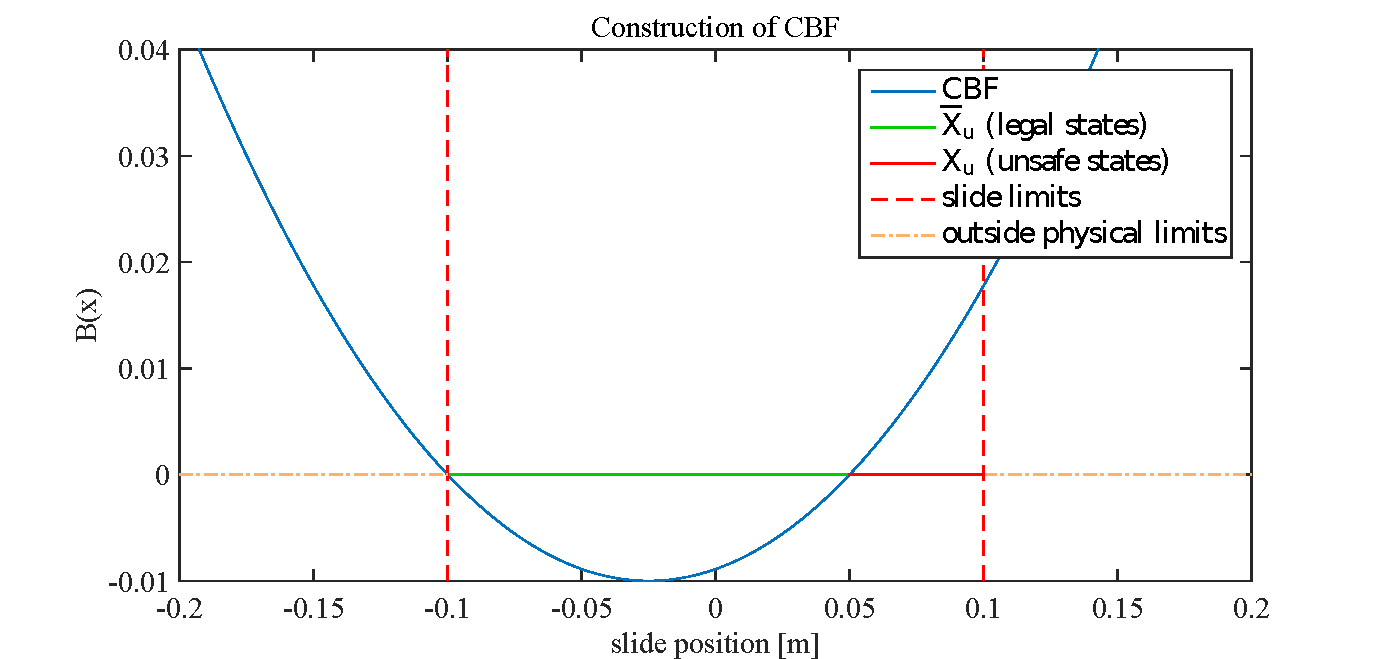
\includegraphics[scale=0.5]{parabel_1.pdf}
\caption{Barrier function along with the $\mathcal{X}_u$ and $\mathcal{X}_u^c$. Plot details and MATLAB script can be found in ????}
\label{fig:barrierfunction}
\end{figure}
\section{Controller Design}
A control laws is now introduced:
\begin{flalign*}
u(x) =
\begin{cases}
	\bar{N}\,x_\text{ref} - K\,x \kk &\text{if $x \in [\Psi_{s-}:\Psi_{s+}]$}\\
	 k_0(x)  \kk &\text{if $x \in [\Psi_{s+}:\Psi_{h+}] \mm \wedge \mm x \in [\Psi_{h-}:\Psi_{s-}]$}
\end{cases}
\end{flalign*}
This can be refined with a parameter $\sigma(x)$ such that the shift between the two control laws is not instantaneous \citep{bib:org_control}. Consider the control law below:
\begin{flalign*}
u(x) = \sigma(x)k_0(x)+(1-\sigma(x))\tilde{u}(x) = \sigma(x)k_0(x)+(1-\sigma(x))(\bar{N} \cdot x_\text{ref}-Kx) 
\end{flalign*}
\vspace{-0.8cm}
\begin{longtable}{p{.9\textwidth} p{.1\textwidth} p{.1\textwidth}} 
Where  & & \\
$u(x)$ is a control signal where safety is ensured  & [$\cdot$] \\
$\tilde{u}(x)$ is a control signal to the linear state space system such that $\tilde{u}=\bar{N}\cdot x_\text{ref}-Kx$ & [$\cdot$] \\ 
$k_0(x)$ is a control law that guarantees safety & [$\cdot$] \\ 
$\sigma(x)$ is a parameter that founds a linear combination between the two control inputs & [$\cdot$] \\ 
$K$ is a constant feedback matrix in $\mathbb{R}^{1 \times 1}$ & [$\cdot$] 
\end{longtable}
\vspace*{-0.2cm}
The control law is thereby a linear combination of two controllers. It is noted that:
\begin{flalign*}
\sigma(x) = 
\begin{cases}
0 \mm &\Rightarrow \mm \text{Pure control by pole placement, i.e. $u(x) = \tilde{u}(x) =  \bar{N}\cdot x_\text{ref}-Kx$ } \\
1 \mm &\Rightarrow \mm \text{Pure control for safety i.e. $u(x) = k_0(x)$ } \\
]0:1[ \mm &\Rightarrow \mm \text{A linear combination of the two control signals $u(x)$ and $\tilde{u}(x)$}
\end{cases}
\end{flalign*}
A block diagram is depicted in \autoref{fig:controlsystem}.
\begin{figure}[H]
	\center
		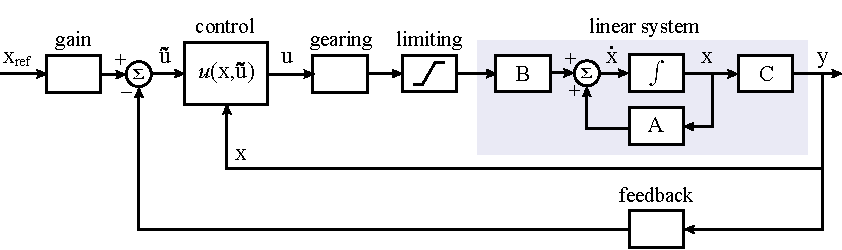
\includegraphics[scale=1]{control_system.pdf}
	\caption{Block diagram of the control system for slide position.}
	\label{fig:controlsystem}
\end{figure}
\subsection{Construction of $k_0$}
The control law ensuring safety can be found as \citep{bib:org_control}:
\begin{flalign}
k_0(x) = \begin{cases}
-\dfrac{L_fB(x)+ \sqrt{(L_fB(x))^2 + \kappa^2(L_gB(x))^TL_gB(x)}}{(L_gB(x))^TL_gB(x)}L_gB(x) &\text{if} \mm L_gB(x) \neq 0 \\
0  &\text{if} \mm L_gB(x) = 0
\end{cases}
\label{eq:control_law}
\end{flalign}
$\kappa$ is a design variable. High values of $\kappa$ implies increased aggressiveness. \Autoref{eq:control_law} ensures indeed safety for the closed loop system $\dot{x} = f_s(x)+g_s(x)k_0(x)$. This is easily proven as:
\begin{flalign*}
L_{f_{cl}}B(x) = L_fB(x) + L_gB(x)k_0(x)
\end{flalign*}
For $L_gB(x) \neq 0:$
\begin{flalign*}
L_{f_{cl}}B(x) &= L_fB(x) + L_gB(x) \left( -\dfrac{L_fB(x)+ \sqrt{(L_fB(x))^2 + \kappa^2(L_gB(x))^TL_gB(x)}}{(L_gB(x))^TL_gB(x)}L_gB(x) \right)  \\
&= L_fB(x) - (L_gB(x))^TL_gB(x) \dfrac{L_fB(x) - \sqrt{(L_fB(x))^2 + \kappa^2(L_gB(x))^TL_gB(x)}}{(L_gB(x))^TL_gB(x)}   \\ 
&= L_fB(x) - L_fB(x) - \sqrt{(L_fB(x))^2 + \kappa^2(L_gB(x))^TL_gB(x)} \\
&= - \sqrt{(L_fB(x))^2 + \kappa^2(L_gB(x))^TL_gB(x)} \mm \leq 0 \mm \forall \mm x
\end{flalign*}
As all terms within the square root are squared, no imaginary numbers occur, as a result $L_{f_{cl}}B(x) \leq 0$ 

According to \autoref{eq:control_law}, when $L_gB(x) = 0$:
\begin{flalign*}
L_{f_{cl}}B(x) = L_fB(x) + L_gB(x)\cdot 0 = L_fB(x)
\end{flalign*}
As $L_fB(x)$ is constructed such that $L_gB(x) = 0 \hspace{0.15cm} \Rightarrow \hspace{0.15cm} L_fB(x) < 0 $. 
\subsection{Construction of $K$ and $\bar{N}$}
No constraints to the constant feedback matrix $K$ will be outlined except stability. It will therefore be determined from the pole placement method such that:
\begin{flalign*}
p_d = 10\cdot \text{eig}(A) \kk \text{where \mm $A = -\tau_s^{-1}$}
\end{flalign*}
Ackermann's formula can be used \citep{bib:acker}.




\chapter{Founding Safety with Static Boundaries}\label{chap:cbf_1d_static}
This chapter intends to implement and analyse a controller ensuring safety if the demands from \autoref{def:cbf} %{req1}, \ref{req2} and \ref{req3} 
are obeyed. This shall first be tested on the slide movement on the Da Vinci surgical robot as it comprises a prismatic joint and a 1:1 mapping from slide $joint\_angle$ to 1D position. Hence any inverse kinematics solver can be bypassed in the early phase of this project which is an important simplification to eliminate initial complications.

The slide movement is visualized in \autoref{fig:slidefig} and an overview of terms used in this section is found in \autoref{fig:safe:overview}, which also encompasses  the case study considered in this chapter. It puts forth the demands that the upper slide region, i.e. the interval $[\Lambda_{h+},\Lambda_\text{lim+}]$ is an unsafe area and the rest is considered safe. Furthermore, everything outside the slide physical limits, i.e. $[-\infty,\Lambda_\text{lim-}]$ and $[\Lambda_\text{lim+},\infty]$ is also considered unsafe. This case study is purely made up with the purpose to demonstrate the use of a safety controller.
\begin{figure}[H]
\centering
\subbottom[Illustration of slide movement.]{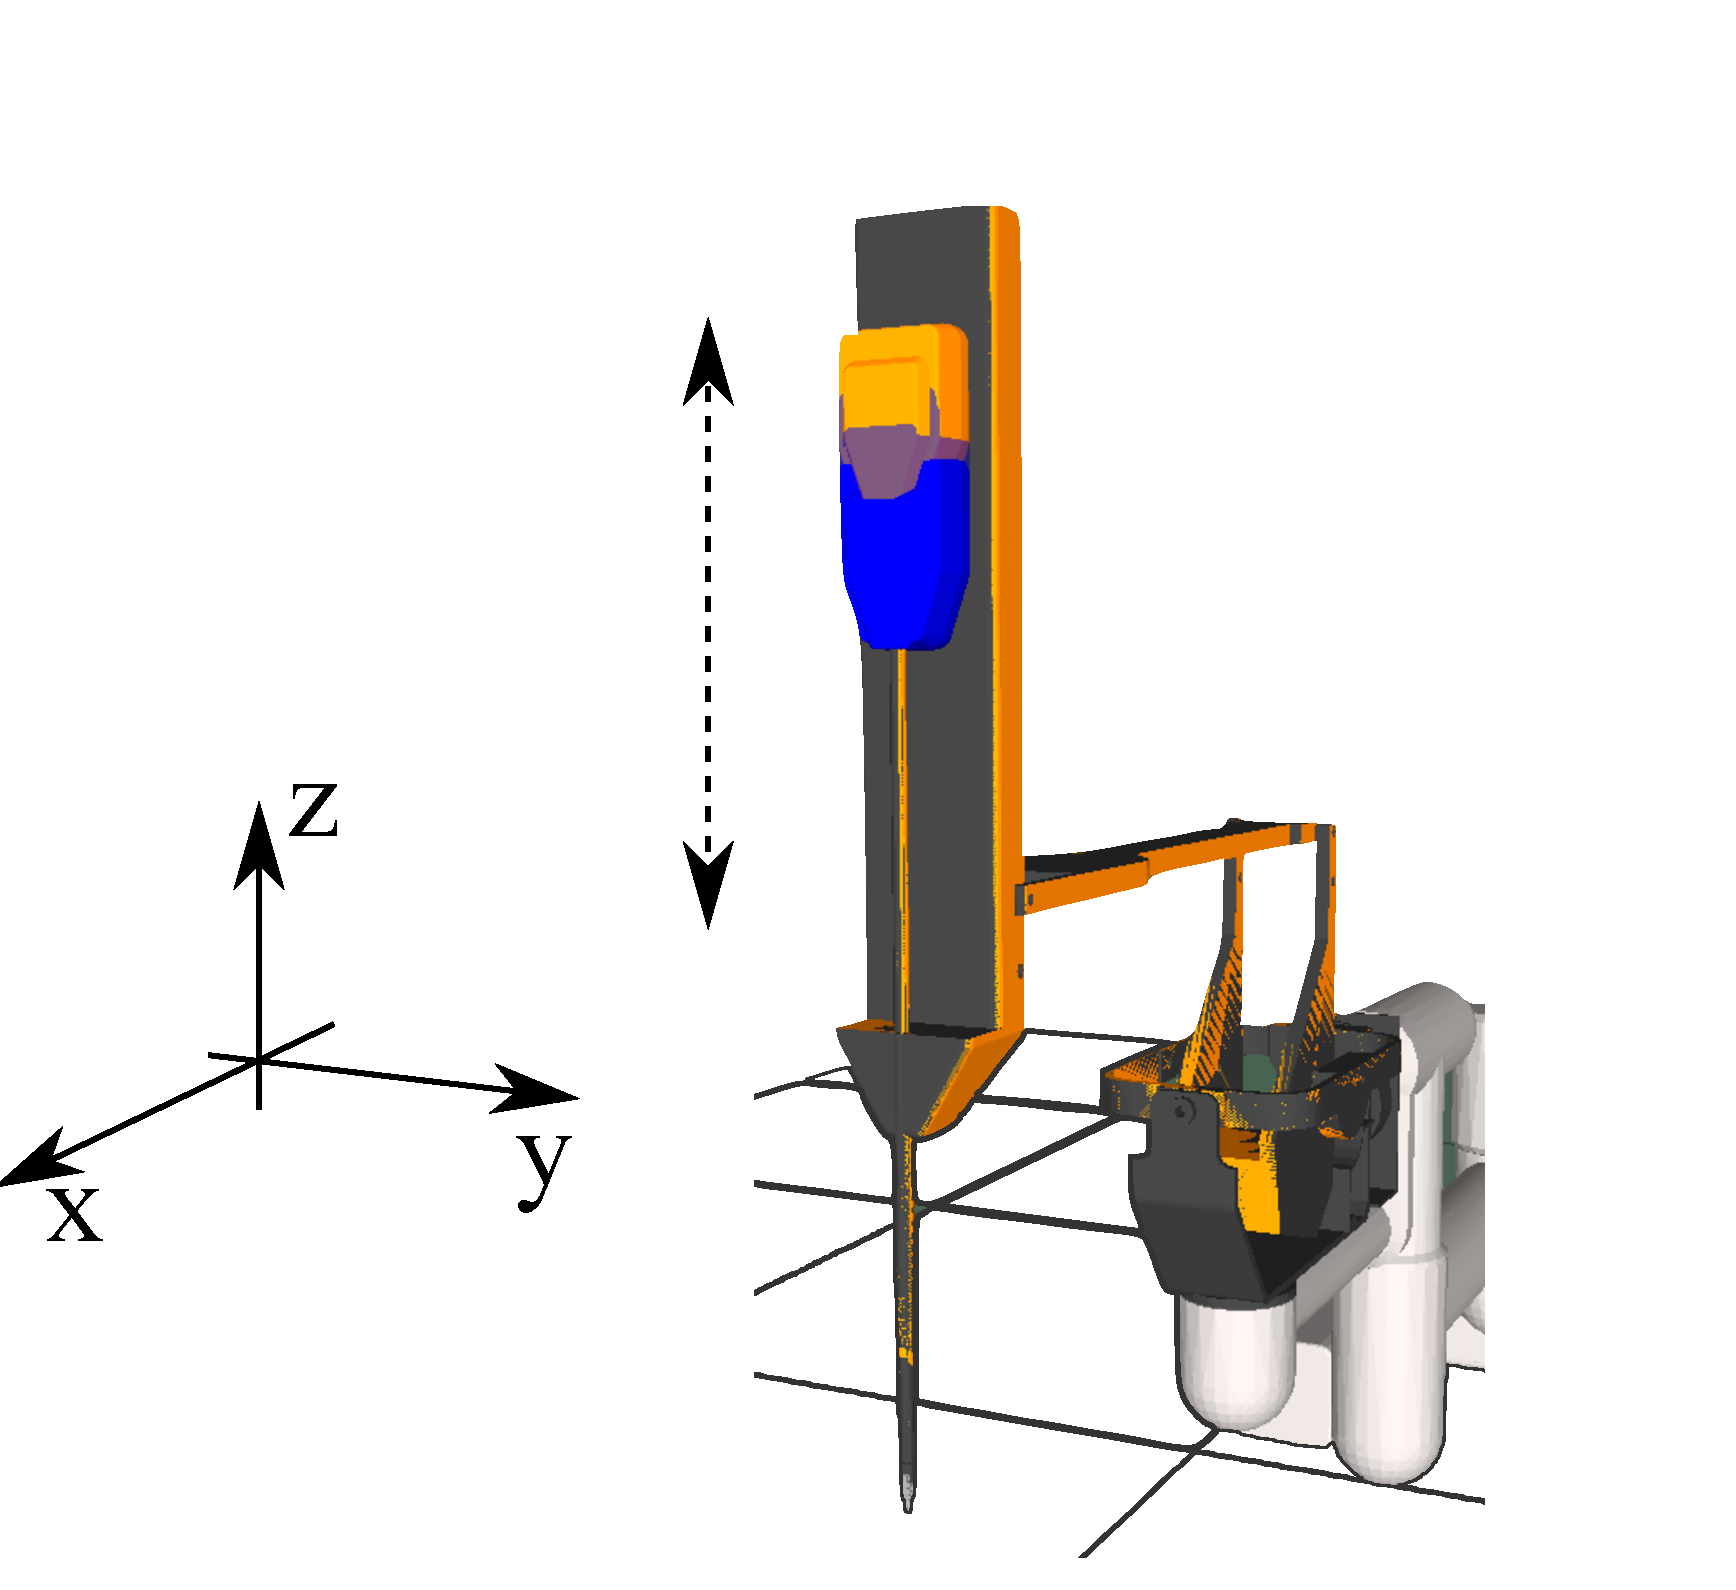
\includegraphics[width=0.46\textwidth]{slidemovefigure.pdf}\label{fig:slidefig}}%
\subbottom[Boundaries used in this section.]{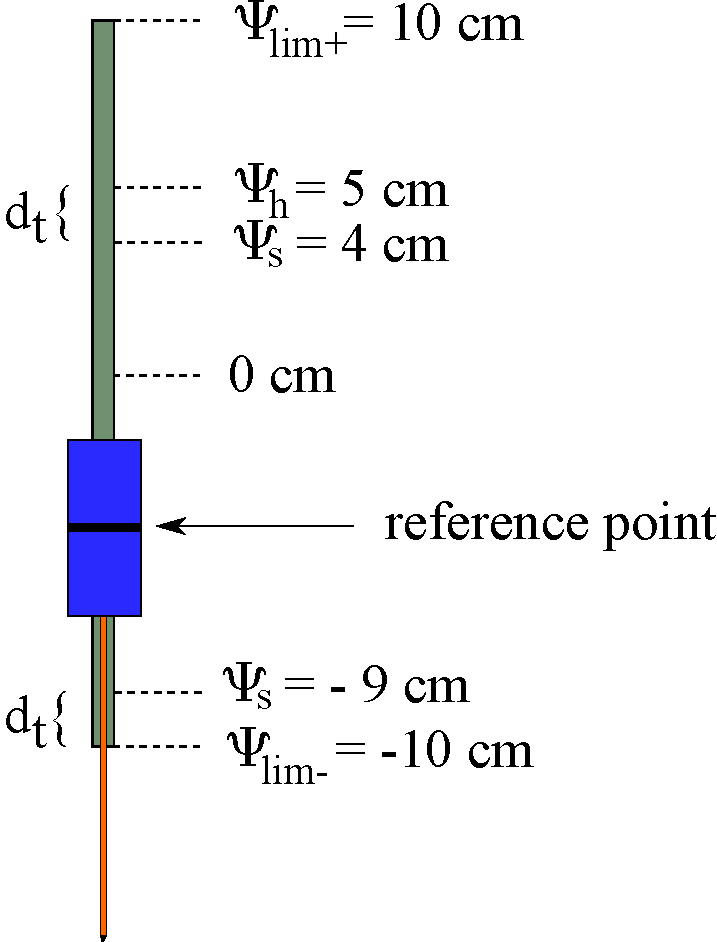
\includegraphics[width=0.42\textwidth]{slide_overview.pdf}\label{fig:safe:overview}}%
\caption{The slide position of the robotic instrument is visualized for the instrument house. As the remaining robot joints are not considered in this chapter, there is a one-to-one translation between instrument house position and instrument tip position. Slide house position in $d_0$ corresponds to tool tip position in zero in the $z$-dimension.}
\label{fig:slide}
\end{figure}
The boundaries for the slide position are summed up in \autoref{tab:intervals}.
\begin{table}[H]
	\begin{tabularx}{\textwidth}{X X X }
\rowcolor{HeaderBlue} 
$\mathcal{X}$ & $\mathcal{X}_u$  & $\mathcal{X}_0$ \\
$x \in \{[\Lambda_{\text{lim}-},\Lambda_{s-}],[\Lambda_{s+},\Lambda_{\text{lim}+}]\}$  & $x \in \{[\Lambda_{\text{lim}-},\Lambda_{h-}],[\Lambda_{h+},\Lambda_{\text{lim}+}]\} $ & $x \in \{[\Lambda_{h-},\Lambda_{s-}],[\Lambda_{s+},\Lambda_{h+}]\}$  \\
\end{tabularx}
\caption{Global state intervals for the position where: $\Lambda_\text{lim}$ is the physical slide limit ($\pm$0.1\,m), $\Lambda_s$ is a soft limit denoting a transition line and $\Lambda_h$ is a hard limit where a trajectory at all cost can not cross. The interval $x \in [\Lambda_{s-},\Lambda_{s+}] = \mathcal{Y}$ is safe thus $\tilde{u}(x)$ stated in \autoref{eq:utilde} can be used in this region.}
\label{tab:intervals}
\end{table}
As the control law stated in \autoref{eq:control_law} utilizes Lie derivatives, a system model is required before any controller design may be initiated.
%\hspace{1cm }\texttt{rostopic echo joint\_states/position[6]} \hspace{0.2cm} {\color{blue}{\# Be sure to have the ROS environment correctly configured according to \autoref{app:ros}}}
\section{Modelling of Slide Movement}\label{sec:model_slide}
To obtain a model of the slide movement, the step response will be measured.  This can be done by subscribing to the \texttt{joint\_state} topic in \gls{ros} (topics are ROS syntax for communication lines, see \autoref{app:ros} for an introduction to ROS). The experiment is described in further details in \autoref{app:meas}, and the result is plotted in \autoref{fig:stepresponseslide}. 
\begin{figure}[H]
\center
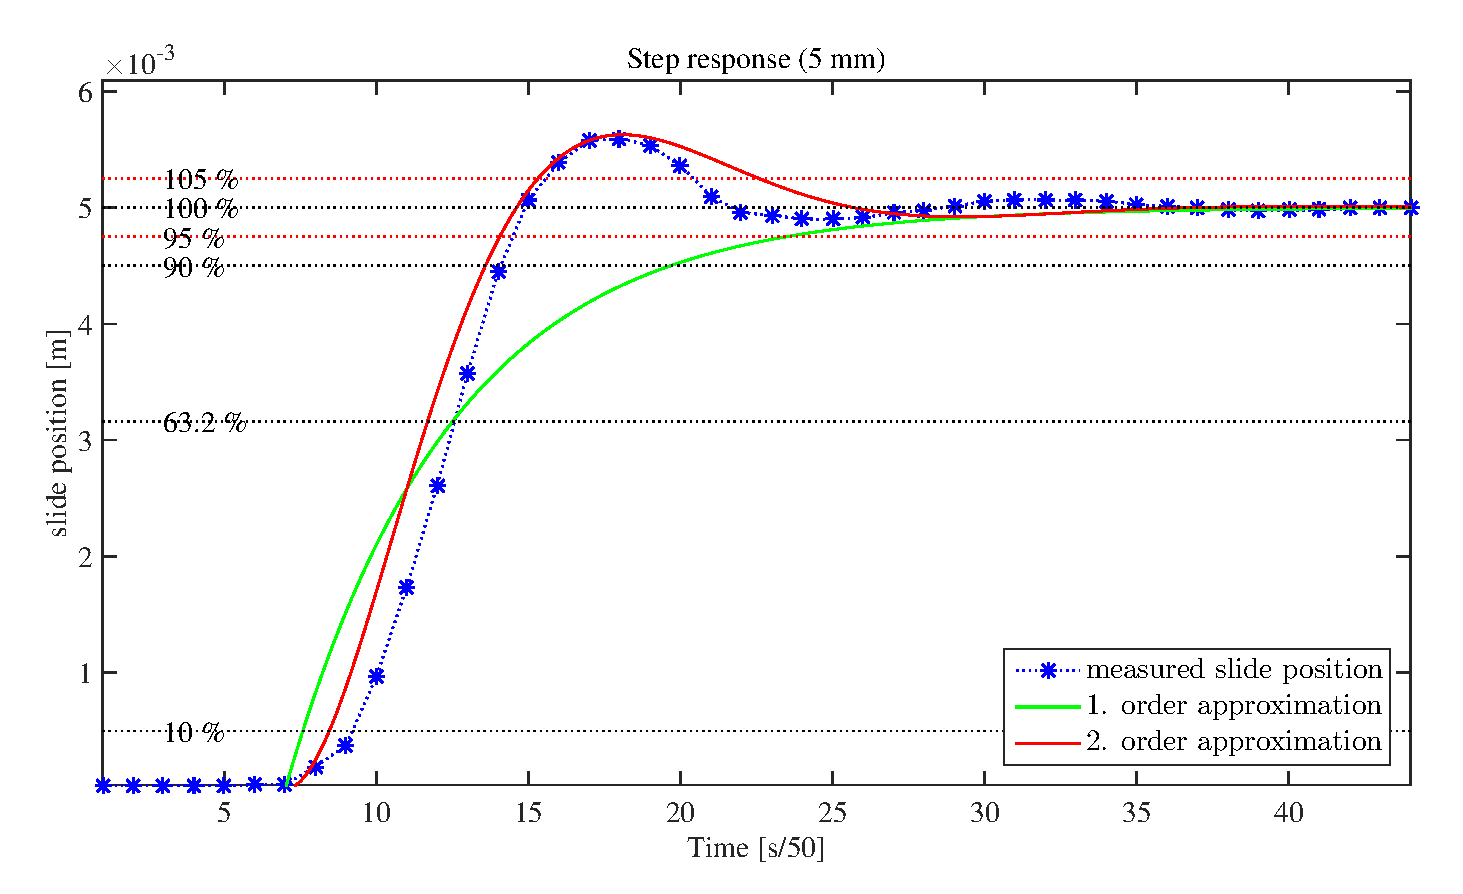
\includegraphics[scale=0.6]{step_slide.eps}
\caption{Step response from 0\,mm to 5\,mm. Plot details and measurements can be found in \autoref{app:cd} as \texttt{matlab\_scripts/slide\_step/plot\_slide\_pos.m}. The experiment is described in \autoref{app:meas}.}
\label{fig:stepresponseslide}
\end{figure}
The system can clearly be approximated with an underdamped second order model, however, for initial simplicity, merely a simple first order model of the slide movement is used. It shall, however, also be approximated as a second order system. This introduces a number of other challenges which is the reason for initial simplicity. These models will throughout this chapter be referred to as:
\begin{itemize}
\item One dimensional (1D) slide movement along the $z$-axis based on \underline{position} only, hence a first order system model.
\item One dimensional (1D) slide movement along the $z$-axis based on \underline{position and velocity}, hence a second order system model.
\end{itemize}
A first order approximation of the state space system will be modelled first. 
\subsection{1D Model based on Position}\label{subsec:model_1d}
The system can be approximated to a linear first order system with a dominating time constant \gls{taus}. The time constant is read from \autoref{fig:stepresponseslide}:
\begin{flalign*}
\tau_s = 110\, \text{ms}
\end{flalign*} 
A linear system can be outlined as:
\begin{flalign}
Y(s) &= \dfrac{1}{\tau_s s + 1}U(s) \nonumber\\
&=  \dfrac{1/\tau_s}{s + 1/\tau_s}\,U(s) = (s+1/\tau_s)^{-1}\,1/\tau_s\,U(s) \qquad\kk \overset{\overset{Y(s)=(\mathbf{C}(s\mathbf{I}-\mathbf{A})^{-1}\mathbf{B}+\mathbf{D})U(s)}{\longrightarrow}}{\scriptsize \text{compare to obtain SS form}}  \nonumber\\ 
& \dot{x} = \underbrace{-\tau_s^{-1}\,x}_{\mathbf{A}x} + \underbrace{\tau_s^{-1}}_{\mathbf{B}} u
\label{eq:1storder_1D_ss}
\end{flalign}
The system matrix $A$ and the input matrix $B$ can be read from the above equation:
\begin{flalign}
\mathbf{A} = - \tau_s^{-1} =  \kk \wedge \kk \mathbf{B} = \tau_s^{-1} \kk \wedge \kk \mathbf{C} = 1 \kk \wedge \kk \mathbf{D} = 0
\end{flalign}
Which completes the first order approximation.

\subsection{1D Model based on Position and Velocity}\label{subsec:model_2d}
The second order approximation is based on the form:
\begin{flalign}
\dfrac{Y(s)}{U(s)} = \dfrac{\omega_n^2}{s^2 + 2\zeta \omega_n s + \omega_n^2}
\label{eq:2order}
\end{flalign}
\begin{tabular}{rll} 
where  & & \\
$Y(s)$ & is the output in the Laplace domain  & [m] \\
$U(s)$ & is the input in the Laplace domain  & [m] \\
\gls{omegan} & is the natural frequency of the system & [rad/s] \\
\gls{zeta} & is the damping coefficient  & [$\cdot$] \\
$s$ & is the Laplace operator  & [rad/s] \\
\end{tabular}\\

The model can unambiguously be approximated from the rise time $t_r$, settling time $t_s$ (5\,\% settling time) and the overshoot $M_p$ \citep{bib:dynamicsystems}. They are measured (conservatively) from \autoref{fig:stepresponseslide} with the purpose to find $\omega_n$ and $\zeta$:
\begin{flalign*}
\omega_n &= \dfrac{1.8}{t_r} = \dfrac{1.8}{0.106\,\text{s}} = 17 \,\text{rad/s} \\
\zeta &= \dfrac{-1}{\omega_n \cdot t_s}\log (0.05) = \dfrac{-1}{17 \cdot 0.320}\log(0.05) = 0.55
\end{flalign*}
\Autoref{eq:2order} can be transformed into state space form: 
\begin{subequations}
\begin{flalign*}
Y(s)s^2 + 2\zeta \omega_n Y(s) s + \omega_n^2 Y(s) - \omega_n^2 U(s)  &= 0 \\
\ddot{y}(t) + 2\zeta \omega_n \dot{y}(t) + \omega_n^2 y(t) - \omega_n^2 u(t) &= 0 
\end{flalign*}
Choose $y(t) = x_1(t) =$ position, and let $\dot{x}_1(t) = x_2(t)$
\begin{flalign}
\begin{bmatrix}
\dot{x}_1(t)\\\dot{x}_2(t)
\end{bmatrix} &= 
\begin{bmatrix}
0 & 1\\
-\omega_n^2  & -2\zeta \omega_n  
\end{bmatrix}
\begin{bmatrix}
x_1(t) \\ x_2(t)
\end{bmatrix} + 
\begin{bmatrix}
0\\\omega_n^2
\end{bmatrix}u(t) \label{eq:2ndorder_1D_ss}\\
y(t) &= 
\begin{bmatrix}
1 & 0
\end{bmatrix}
\begin{bmatrix}
x_1(t) \\ x_2(t)
\end{bmatrix}
\end{flalign}
\end{subequations}
\begin{tabular}{rll} 
where  & & \\
\gls{x1}$(t)$ & is the position& [m] \\
\gls{x2}$(t) = \dot{x}_1(t)$ &is the velocity  & [m/s] \\
$y(t)$ & is the output (slide position)  & [m] \\
$u(t)$ & is the control input  & [$\cdot$]\\
\end{tabular}\\

Thus the linear system matrices can be outlined as:
\begin{flalign}
\mathbf{A} = \begin{bmatrix}
0 & 1\\
 -\omega_n^2   & -2\zeta \omega_n 
\end{bmatrix} \kk \wedge \kk \mathbf{B} = \begin{bmatrix}
0 \\ \omega_n^2
\end{bmatrix} \kk \wedge \kk \mathbf{C} = \begin{bmatrix}
1 & 0
\end{bmatrix} \kk \wedge \kk \mathbf{D} = 0 \label{eq:system:2}
\end{flalign}
Which completes the second order model.

\section{Construction of CBF}\label{sec:construct_cbf}
To illustrate the usefulness of \glspl{cbf}, a palpable example hereof will be created with direct application to the Da Vinci robot. This example does not directly constitute application to a patient but favour the theory in a neat and comprehensible sense and secure a way to visually and physically verify the method.
%
%Consider the state intervals defined in \autoref{tab:intervals}.
%
%
\subsection{Construction of CBF based on First Order Model}\label{subsec:cbf-1order}
In this subsection, the state vector $x \in \mathbb{R}$ consists of the position only. Thus, a parabola is now introduced as \gls{cbf} as it allows an easy way to define $\mathcal{X}_u$ and $\mathcal{X}_0$ from \autoref{tab:intervals}. %A coordinate shift is performed such that the slide movement occurs along the $x$-axis instead of the $z$-axis. 
\begin{flalign}
B(x) &= ax^2+bx+c \label{eq:cbf1} 
\end{flalign}
The parameters $a$, $b$ and $c$ can be easily chosen to fulfil the requirements in \autoref{cer1} and \ref{cer2} for a barrier function, thereby fulfilling the parallel requirements for the \gls{cbf} in \autoref{req1} and \ref{req3}. From \autoref{req2} it is required that either $L_gB(x) \neq 0 \,\,\,\forall x\in \mathcal{X}$, or that $L_fB(x)<0$ when $L_gB(x) = 0$, as the input in that case will be insignificant. Analysing $L_gB(x) = 0$
\begin{flalign*}
	L_gB(x) \Bigm|_{g(x)=\mathbf{B}} = ( 2ax + b ) \cdot \tau^{-1} = 0 \kk \Rightarrow \kk x = \dfrac{-b}{2a}\label{eq:LgB_1D}
\end{flalign*}
it is seen that this is only the case in $x = \tfrac{-b}{2a}$ which is indeed the critical point for a one dimensional parabola. As is the case for Lyapunov functions (see  \autoref{eq:lyap_vdot_minus_criticalpoint}) in the critical point the requirement on the derivative is relaxed to  $L_fB(x) \leq 0$.   
\begin{flalign}
L_fB(x) = \dfrac{d}{dx}B(x)f(x)\Bigm|_{f(x)=\mathbf{A}x}  &= (2ax+b)(-\tau^{-1}x) = -2\tau^{-1}ax^2-\tau^{-1}bx \nonumber\\
L_fB(x)\Bigm|_{x= \frac{-b}{2a}} &= -2\tau^{-1}a\left(\frac{-b}{2a}\right)^2-\tau^{-1}b\left(\frac{-b}{2a}\right) = 0\nonumber
%0 \kk \Leftrightarrow \kk  -2\tau^{-1}ax^2-\tau^{-1}bx = 0 \nonumber
% \\  &-2ax^2-bx = 0 \mm \Rightarrow \mm x = 
%\begin{cases}
%  \frac{-b}{2a} \\
%   0   
%\end{cases}
\label{eq:interval1}
\end{flalign}
Hence the \gls{cbf} is valid for all choices of $a,b$. The scalar $c$ must be less than zero to comply with \autoref{req3}.
At this point in time, three equations with three unknowns can be outlined to fulfil the initial demand in \autoref{fig:safe:overview}.
\begin{flalign*}
 \left.
 \begin{aligned}
a\,\Lambda_{h+}^2 + b\,\Lambda_{h+} + c = 0 \\
a\,\Lambda_{h-}^2 + b\,\Lambda_{h-} + c = 0 \\
a\left( \frac{\Lambda_{h-}+\Lambda_{h+}}{2}\right)^2 + b\left(\frac{\Lambda_{h-}+\Lambda_{h+}}{2}\right) + c = \underbrace{-0.025}_\text{any constant $<0$} 
\end{aligned}
\mm \right\}
 \qquad \begin{matrix}
 a &= \,\,\,\,\,\,\,\,1.7778 \\ b &= \,\,\,\,\,\,\,\,0.0889 \\ c &= -0.0089
 \end{matrix}
\end{flalign*}
%The interval where $B(x)$ is invalid can thereby be found from \autoref{eq:interval}:
%\begin{flalign*}
%B(x) \hspace{0.15cm} \text{invalid:} \mm  x \in [-0.0250,0] \kk \text{if} \mm L_gB(x) = 0
%\end{flalign*}
%However, this is indifferent as $\{\mathcal{X} \,\bigcap\, [\Lambda_{s-},\Lambda_{s+}]  \} = \emptyset $. Thus the barrier function is a valid \gls{cbf}. It is plotted in \autoref{fig:barrierfunction}
The \gls{cbf} is plotted in \autoref{fig:barrierfunction} from which it is seen that the demands from \autoref{tab:intervals} are fulfilled.
\begin{figure}[H]
\center
	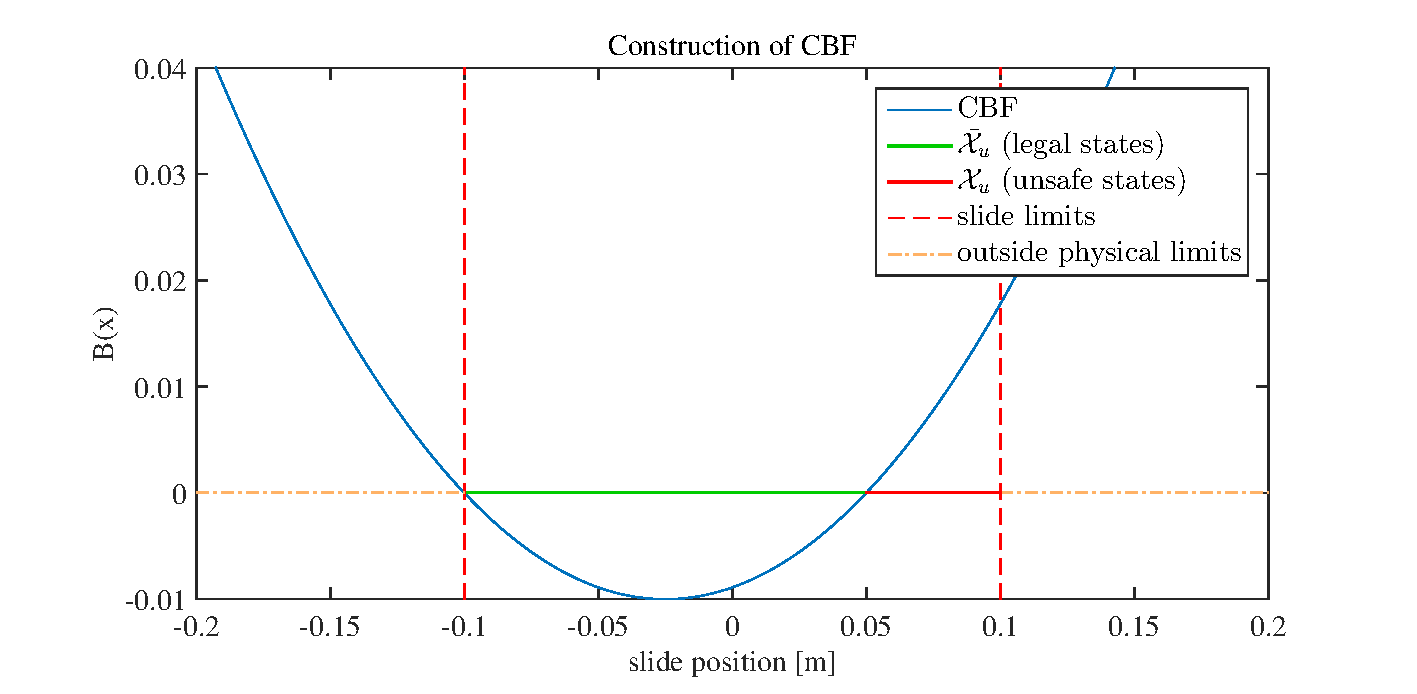
\includegraphics[scale=0.63]{parabel_1.eps}
	\caption{Barrier function shown along with the $\mathcal{X}_u$ and $\mathcal{X}_u^c$. Plot details and MATLAB script can be found in \autoref{app:cd} as \texttt{matlab\_scripts/plot\_parabola/plot\_parabola.m}}
	\label{fig:barrierfunction}
\end{figure}
%\underline{Note:} The above analysis ensures safety regardless of $L_gB(x) = 0$ as it merely takes place at the critical point, i.e.:
%\begin{flalign*}
% L_gB(x) = (2ax+b)B = 2ax\tau^{-1} + b\tau^{-1} = 0 \kk \Leftrightarrow \kk 2ax = -b \kk \Leftrightarrow \kk x = \dfrac{-b}{2a}
% \end{flalign*} 
% This is again the parabola extremity as it was found in \autoref{eq:interval1} and in fact an allowed exception for condition \autoref{req2} as the system is in its equilibrium.

\subsection{Construction of CBF Based on Second Order model}\label{subsec:cbf-2order}
Consider now for the second order system the same candidate \gls{cbf} as given in \autoref{eq:cbf1}. Note that $B(x_1)$ is a function of position only, such that the CBF is:
\begin{flalign*}
B(x_1) = a\,x_1^2+ b\,x_1 + c
\end{flalign*}
For this system model the Lie derivative $L_gB(\mathbf{x})=0\,\,\forall \mathbf{x}$:
\begin{flalign*}
L_gB(\mathbf{x}) = \dfrac{d B(x_1)}{d \mathbf{x}}g(\mathbf{x}) \Bigm|_{g(\mathbf{x})=\mathbf{B}} =  
\begin{bmatrix}
\dfrac{\partial B(x_1)}{\partial x_1} & \dfrac{\partial B(x_1)}{\partial x_2} 
\end{bmatrix}\begin{bmatrix}
0 \\ \omega_n^2
\end{bmatrix} = 0 \label{eq:LgB_secondorder_invalid}
\end{flalign*}
This puts forth the requirement that $L_fB(\mathbf{x})<0\,\,\, \forall \, \mathbf{x}$. Accordingly:
\begin{flalign*}
L_fB(\mathbf{x}) = \dfrac{d B(x_1)}{d \mathbf{x}}f(\mathbf{x}) \Bigm|_{f(\mathbf{x})=\mathbf{Ax}} &= 
\begin{bmatrix}
\dfrac{\partial B(x_1)}{\partial x_1} & \dfrac{\partial B(x_1)}{\partial x_2} 
\end{bmatrix}
\begin{bmatrix}
0 & 1 \\
-\omega_n^2 & -2\zeta\omega_n
\end{bmatrix} \begin{bmatrix}
x_1 \\ x_2
\end{bmatrix} \nonumber \\
&= (2ax_1+b) x_2 - 0\cdot(\omega_n^2 x_1 + 2\zeta \omega_n x_2) \nonumber \\
&= 2ax_1x_2 + bx_2
\label{eq:2d_x1}
\end{flalign*}
Note that the velocity appears in both terms. As the velocity can be both decreasing and increasing for all positions, this demand is impossible to fulfil with this candidate \gls{cbf}  and it is therefore invalid. A solution may be to include the velocity in the barrier function. 

Safety constraints on velocity are not of any significant importance as such, but they are necessary for $L_gB(\mathbf{x})$ to obtain values different from zero as opposed to the Lie derivative of the invalid \gls{cbf} $B(x_1)$.
Consider instead the elliptic paraboloid as \gls{cbf}:
\begin{flalign}
B(x_1,x_2) =  \left( \dfrac{(x_1-x_{10})^2}{a_2^2} + \dfrac{(x_2-x_{20})^2}{b_2^2} \right) c_1 + c_2
\label{eq:cbf2}
\end{flalign}
\begin{tabular}{rp{13.7cm}l} 
where  & & \\
$x_1$& is the position  & [m] \\
$x_2$& is the velocity & [m/s] \\
$x_{10}$& is the extremity point for $x_1$ and thereby equilibrium point for an upward paraboloid & [m] \\
$x_{20}$& is the extremity point for $x_2$ and thereby equilibrium point for an upward paraboloid & [m/s] \\
$a_2$& is a constant that dictates the level of curvature in the $x_1-B(\textbf{x})$ plane & [$\cdot$] \\
$b_2$& is a constant that dictates the level of curvature in the $x_2-B(\textbf{x})$ plane & [$\cdot$] \\
$c_1$ & is a constant that dictates if the paraboloid points upward ($c_1>0$) or downward ($c_1 < 0$)& [$\cdot$]  \\
$c_2$ & is a constant that dictates the offset in $B(\textbf{x})$ axis & [$\cdot$] \\
\end{tabular}\\

The elliptic paraboloid allows constraints on both position and velocity.  To ensure that the position demands from \autoref{tab:intervals} are still fulfilled and are so for all possible velocities (constrained by the slide movement's physical limits), the below values are chosen:
\begin{flalign*}
x_{10} &= \dfrac{\Lambda_{h-}+\Lambda_{h+}}{2} = -0.025 \\
x_{20} &= 0\\
M_{0} &= 4
%\Lambda_{x2-} &= -4 \kk \text{denotion of the lowest value where $B(0,x_2)=0$} \\
%\Lambda_{x2+} &= 4 \kk \text{denotion of the highest value where $B(0,x_2)=0$} 
\end{flalign*}
\begin{figure}[htbp]
	\centering
	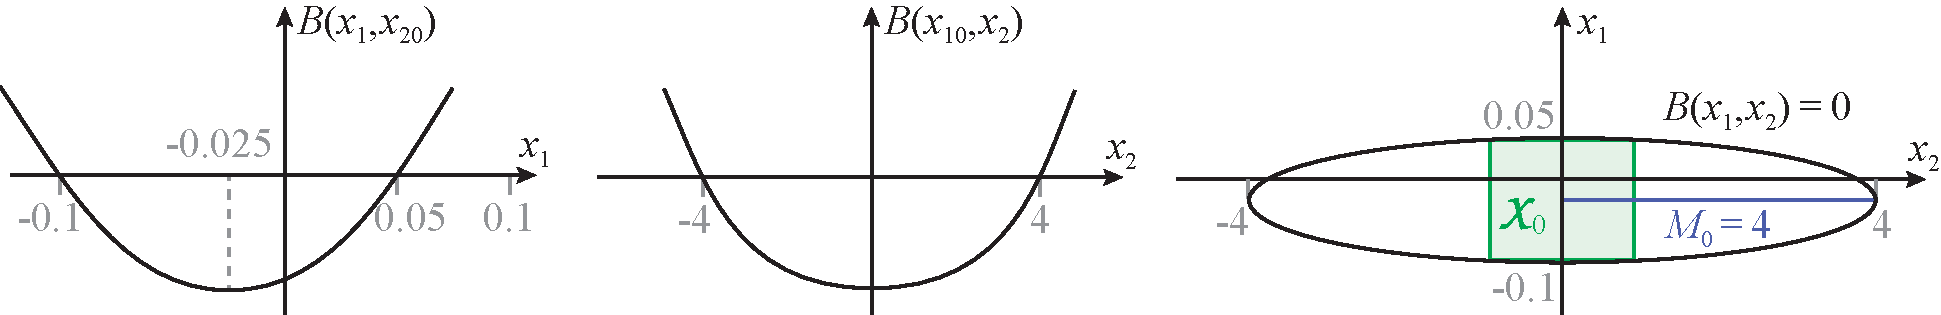
\includegraphics[width=\textwidth]{cbf_2ndorder.pdf}
	\caption{Choice of critical point coordinate $x_{10}$  as the middle of the safe position interval. The semimajor axis of the \gls{cbf}'s zero level set is chosen much larger than the physical limits  of the slide velocity.}
	\label{fig:cbf_2ndorder}
\end{figure}

where ${M}_0$ denotes the semimajor axis of the zero level set of the \gls{cbf}.
Note that $x_{20}$ ensures velocity equilibrium in 0\,m/s and note that the velocity outermost points are determined far bigger than the robot's physical limits to ensure that all position values on the interval  $[-0.1\,\,\,\,0.05]$ are considered safe (almost) independently of the velocity. % $\mathcal{X}_0 \notin \mathcal{X}_u $. 
This is sketched in \autoref{fig:cbf_2ndorder} along with the chosen values.

Having chosen the coordinates $x_{10}$ and $x_{20}$ for the critical point, an arbitrary negative value is chosen for $B(x_{10},x_{20})$, and using the four known coordinates from the zero level set $(\Lambda_{h+},x_{20})$, $(\Lambda_{h-},x_{20})$, $(x_{10},-M_0)$ and $(x_{10},M_0)$, five equations with four unknowns can be outlined with the below numerical values.
\vspace{-3mm}
\begin{flalign*}
\hspace{5mm} \left.
\begin{aligned}
\left( \dfrac{\left(\frac{\Lambda_{h-}+\Lambda_{h+}}{2}-x_{10}\right)^2}{a_2^2} + \frac{(0-x_{20})^2}{b_2^2} \right)c_1 + c_2 =  \underbrace{-1.000}_\text{any constant $<0$} \\
\left(\dfrac{(\Lambda_{h+}-x_{10})^2}{a_2^2} +\frac{(0-x_{20})^2}{b_2^2}\right) c_1 + c_2 = 0 \\
 \left(\dfrac{(\Lambda_{h-}-x_{10})^2}{a_2^2}+\frac{(0-x_{20})^2}{b_2^2}\right) c_1 + c_2 = 0 \\
 \left(\dfrac{\left(\frac{\Lambda_{h-}+\Lambda_{h+}}{2}-x_{10}\right)^2}{a_2^2} +\dfrac{(4-x_{20})^2}{b_2^2} \right)c_1 + c_2 = 0 \\
\left(\dfrac{\left(\frac{\Lambda_{h-}+\Lambda_{h+}}{2}-x_{10}\right)^2}{a_2^2} + \dfrac{(-4-x_{20})^2}{b_2^2}\right) c_1 + c_2 = 0 
% \dfrac{\left(0-x_{20}\right)^2}{b_2^2} c_1 + c_2 =  \underbrace{-1.000}_\text{any constant $<0$}  
\end{aligned}
\mm \right\}
 \qquad 
\begin{matrix*}[r]
x_{10} &=& -0.025 \\ 
x_{20} &=&  0.000 \\
B(x_{10},x_{20}) &=&   -1.000\\
&&\\
a_2 &=& 0.075 \\ 
b_2 &=& 4.000 \\
c_1 &=& 1.000 \\ 
c_2 &=& -1.000
\end{matrix*}
\end{flalign*}
The Lie derivatives can now be calculated as:
\begin{flalign}
L_gB(\mathbf{x}) &= \dfrac{d B(x_1,x_2)}{d \mathbf{x}}  g(\mathbf{x}) \Big|_{g(\mathbf{x})=\textbf{B}} = \begin{bmatrix}
\dfrac{\partial B(x_1,x_2)}{\partial x_1} & \dfrac{\partial B(x_1,x_2)}{\partial x_2}
\end{bmatrix}  \begin{bmatrix}
0 \\ \omega_n^2
\end{bmatrix} \nonumber \\
 &= \begin{bmatrix}
 \dfrac{c_1(2x_1 - 2x_{10})}{a_2^2} &  \dfrac{c_1(2x_2 - 2x_{20})}{b_2^2}
\end{bmatrix}  \begin{bmatrix}
0 \\ \omega_n^2
\end{bmatrix} = 
\dfrac{c_1\omega_n^2(2x_2-2x_{20})}{b_2^2} \Bigm|_{x_{20}=0} \nonumber\\
&= \dfrac{2c_1\omega_n^2}{b_2^2} x_2
\label{eq:LgB_2}
\end{flalign}
It is seen that $L_gB(\mathbf{x}) \neq 0 \mm \forall \,\,\, x_2 \neq 0$, hence $L_fB(\mathbf{x})$ is for that reason analysed and evaluated at $x_2=0$:
%\vspace{-3mm}
\begin{flalign}
L_fB(\mathbf{x}) &= 
\dfrac{\partial B(x_1,x_2)}{\partial \mathbf{x}} f(\mathbf{x})
\Big|_{f(\mathbf{x}) = \textbf{\textbf{Ax}}} =
\begin{bmatrix}
\dfrac{\partial B(x_1,x_2)}{\partial x_1} & \dfrac{\partial B(x_1,x_2)}{\partial x_2}
\end{bmatrix} 
\begin{bmatrix}
0 & 1 \\
-\omega_n^2 & -2 \zeta \omega_n
\end{bmatrix} 
\begin{bmatrix}
x_1 \\ x_2
\end{bmatrix} \nonumber\\
&= \begin{bmatrix}
 \dfrac{c_1(2x_1 - 2x_{10})}{a^2} &  \dfrac{c_1(2x_2 - 2x_{20})}{b^2}
\end{bmatrix} 
\begin{bmatrix}
x_2 \\ -\omega_n^2 x_1 - 2\zeta \omega_n x_2
\end{bmatrix} \nonumber\\
&= \dfrac{c_1x_2(2x_1-2x_{10})}{a_2^2} - \dfrac{c_1(2x_2-2x_{20})(\omega_n^2 x_1+2\zeta \omega_n x_2 )}{b_2^2} \Big|_{x_{20} = 0} \nonumber\\
&= 2c_1\left( \dfrac{x_1-x_{10}}{a_2^2} - \dfrac{\omega_n^2 x_1 +2\zeta \omega_n x_2}{b_2^2} \right) x_2 \Big|_{x_{2} = 0} = 0
\label{eq:LfB_2}
\end{flalign}
It is noted that $L_fB(\mathbf{x}) = 0$ for $x_2 = 0$ which implies stability but not asymptotic stability. That is in general not good for physical systems and does not fulfil \autoref{req2}. It does, however, fulfil \autoref{req2_weak} thus proving $B(x_1,x_2)$ to be a weak \gls{cbf}. %However, an engineering reflection and decision is taken at this point.
Note that when the velocity is zero, the slide movement is steady, although only marginally stable. %At this point $k_0(x)=0$, which indeed will force the slide movement to its origin as the control signal is the reference to a position controller. 
As an engineering reflection it is considered that when the state leaves the marginally stable equilibrium, $x_2 \neq 0$, and the safety controller  will ensure that the state will increase its distance to the unsafe set and go towards its stable equilibrium in $(x_{10},x_{20})=(-0.025,0)$. 
%It implies hereafter $x_2 \neq 0$ again which is sufficient for the safety controller. %That is in this case a good thing as the slide will move back to the safe region and away from $\Lambda_{h-}$ and $\Lambda_{h+}$. Lastly, the velocity will never be truly zero due to the finite resolution, i.e. a finite sampling rate. For these reasons, the \gls{cbf} from \autoref{eq:cbf2} is accepted, well aware that the \gls{cbf} is insufficient,. It is, however, important to keep in mind that this is a dangerous decision. {\color{green}{RAFAL: Er det overhovedet OK at sige s\aa dan?}}


\begin{figure}[H]
\hspace*{-2mm}
	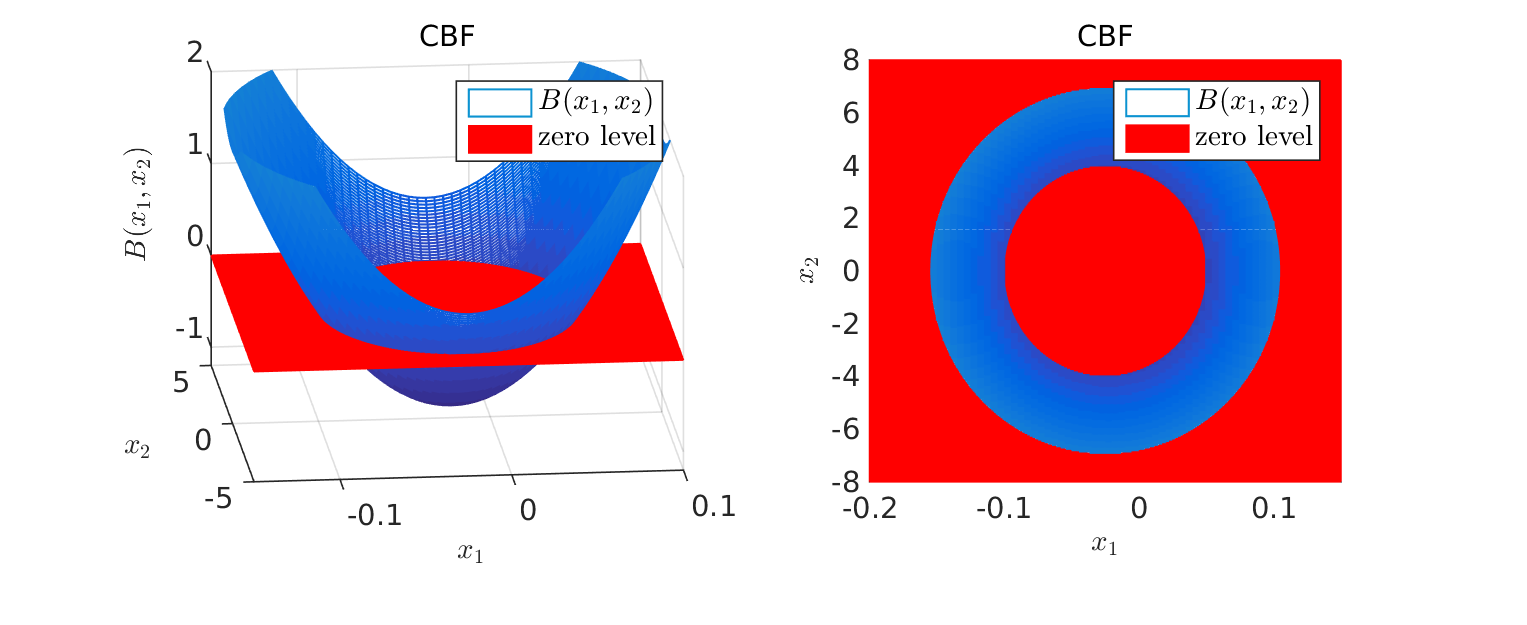
\includegraphics[width=1.02\textwidth]{cbf_2d.eps}
	\vspace*{-11mm}
	\caption{CBF for the second order system model. Plot details and MATLAB script can be found in \autoref{app:cd} as \texttt{matlab\_scripts/plot\_cbf\_2d/plot\_cbf\_2d.m}}
	\label{fig:barrierfunction_2d}
\end{figure}
The elliptic paraboloid with its proper boundaries is plotted in \autoref{fig:barrierfunction_2d}, from which it is seen how $B(x_1,x_2)<0$ only within the specified regions, i.e. $x_2 \in [-M_0,M_0]$ and $x_1 \in [\Lambda_{h-},\Lambda_{h+}]$. %, and thus everything else is unsafe, i.e. $B(x) > 0$. 
It is also seen that for small velocities (physically $x_{2,\text{max}}\approx 1$\,m/s) the \gls{cbf} is approximately vertical in the boundaries of $x_1$ %when the big numerical difference in the axes is taken into account.
leaving $\mathcal{X}_0$ almost independent of the velocity, as prescribed in \autoref{fig:cbf_2ndorder}.

\begin{figure}[H]
	\centering
	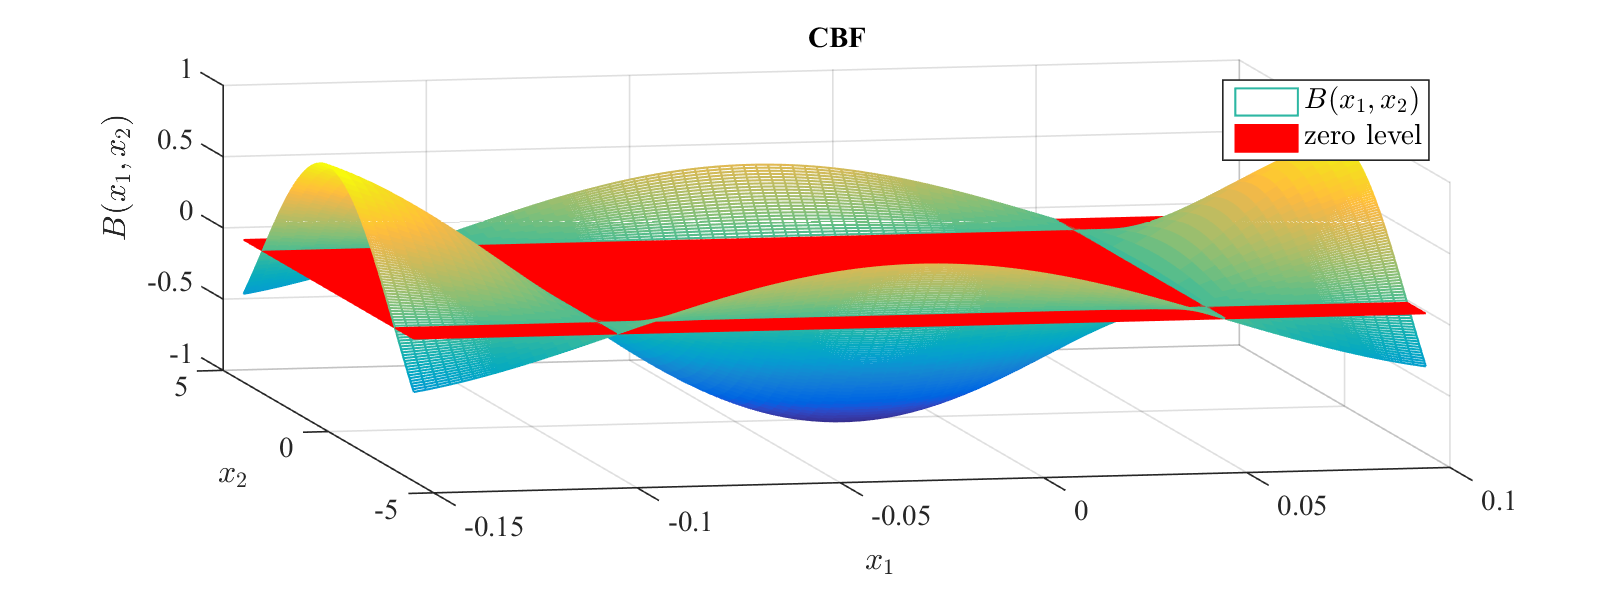
\includegraphics[width=.95\textwidth]{cbf_example_sinus.eps}
	\caption{CBF. Example to demonstrate how other CBFs suffer when $x_2 = 0$.}
	\vspace{-7mm}
	\label{fig:barrierfunction_example_sinus}
\end{figure}
\vspace{5mm}

\textbf{\underline{\textit{Remark:}}} The issue caused by $x_2=0$ is not only the case for this specific \gls{cbf} but for many \gls{cbf}s. Take for example another CBF that could fulfil the position requirements from \autoref{tab:intervals}:
\begin{flalign*}
B(x_1,x_2) = \cos (c_3 x_1 + c_4) \cdot \cos (c_5 x_2 + c_6)
\end{flalign*}
It turns out that the coefficients $c_3 = 21.00, c_4 = 119.91, c_5 = 0.50, c_6 = 3.15$ induce a CBF with the same properties as the one depicted in \autoref{fig:barrierfunction_2d}. The \gls{cbf} is outlined graphically in \autoref{fig:barrierfunction_example_sinus}.

Thus $L_gB(x_1,x_2)$ can be found as:
\begin{flalign*}
L_gB(x_1,x_2) = -c_5 \omega_n^2 \cos (c_3 x_1+c_4)\sin(c_5 x_2+c_6)
\end{flalign*}
Now note that $L_gB(x_1,x_2) = 0$ when $c_6+c_5x_2 = i\pi$, $i\in\mathbb{Z}$, which is true for e.g. $x_2 \approx 0$. This implies the requirement that $L_fB(x_1,x_2) < 0$ whenever $x_2 \approx 0$. % As $L_gB(x_1,x_2) \neq 0 \,\, \forall \,\, x_2 \approx 0$, requirements for $L_fB(x_1,x_2)$ is necessary. 
However, taking a look at $L_fB(x_1,x_2)$:
\begin{flalign*}
L_fB(x_1,x_2) = 
c_5\cos (c_3 x_1+c_4 ) \sin(c_5 x_2+c_6)( \omega_n^2 x_1 + 2  \zeta \omega_n x_2) - c3 x_2 \cos( c_5 x_2+c_6) \sin( c_3 x_1+c_4)
\end{flalign*}
quickly poses the fact that $L_fB(x_1,x_2 )$ is not necessarily negative for $x_2 \approx 0$ due to the sign alternation caused by the term $\sin(c_3 x_1+c_4)$ in the boundaries.

\section{Control Design}
\vspace*{-1mm}
This section constitutes the design of the two controllers. The controller based on the first order approximation is straight forward whereas the controller based on the second order approximation requires an observer because the velocity cannot be measured.
\subsection{Control Design based on First Order
	\vspace*{-1mm} Model}\label{sec:K_Nbar_1D_1storder}
To be able to find $k_0(x)$ from \autoref{eq:control_for_safety}, the constant $\epsilon$ used in \autoref{eq:smoothness} must be found. It can be determined from the \gls{cbf} from \autoref{eq:cbf1} such that it complies with the requirements from \autoref{tab:intervals}:
\begin{flalign}
\epsilon = |B(\Lambda_{s+})| = |B(\Lambda_{s-})| = 0.00249
\label{eq:epsilon}
\end{flalign}
Utilizing $\sigma(x)$ as described in \autoref{eq:smoothness} secures a neat way to incorporate the transition between $\Lambda_s$ and $\Lambda_h$ because the safety controller $k_0(x)$ gradually takes over when the trajectory exceeds $\Lambda_s$. \Autoref{fig:epsilon_plot} illustrates how $\epsilon$ and $B(x)$ are connected.
\begin{figure}[H]
	\center
		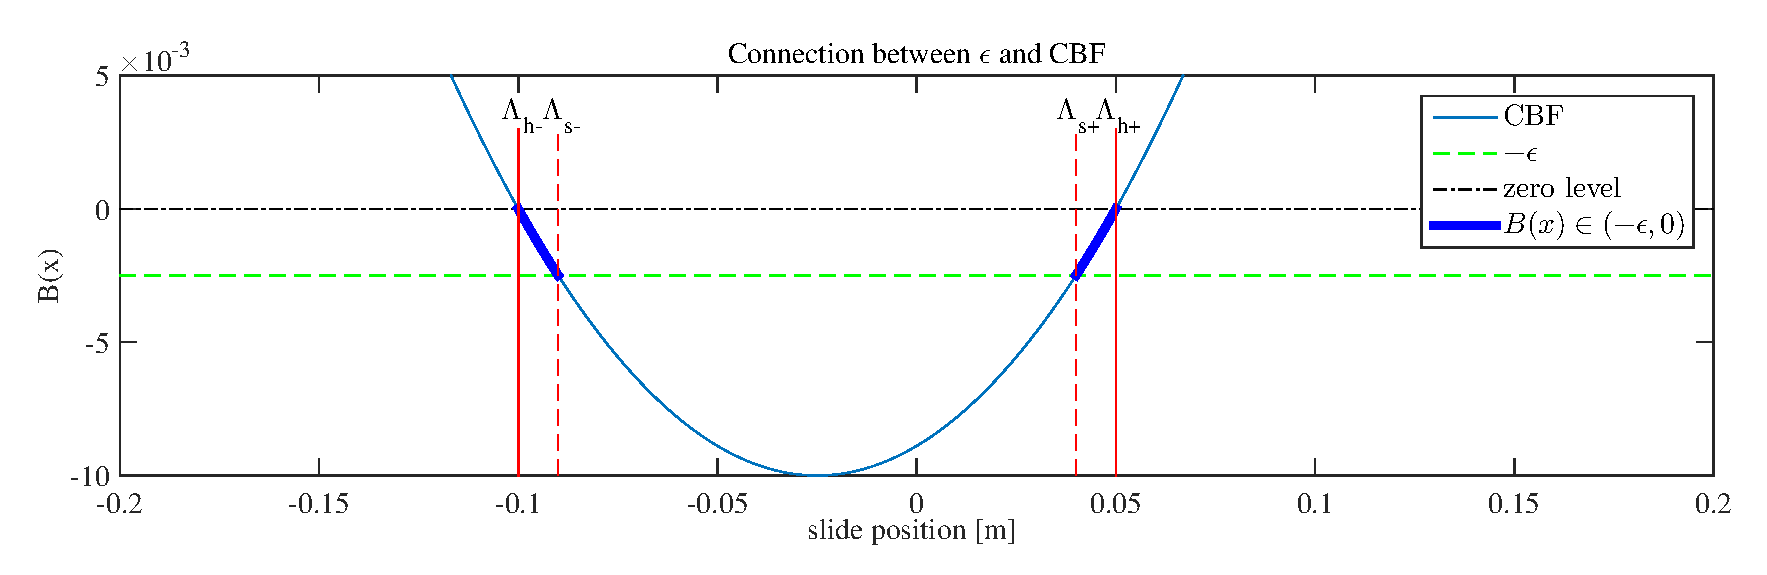
\includegraphics[scale=0.55]{epsilon_plot.eps}
	\caption{Connection between $\epsilon$ and CBF. MATLAB script and plot details can be found in \autoref{app:cd} as \texttt{matlab\_scripts/plot\_epsilon/plot\_epsilon\_slide\_1d.m}}
	\label{fig:epsilon_plot}
\end{figure}

The system is approximated as a linear system on the form $\dot{\mathbf{x}}=\textbf{Ax}+\textbf{Bu}$, thus pole placement can be used. No constraints to the constant feedback matrix $\mathbf{K}$ will be outlined except stability. It will therefore be determined from the pole placement method where a closed loop pole that is ten times faster than the open loop pole will be placed. Ackermann's formula can be used \citep{bib:acker}:
\begin{enumerate}
\itemsep-3mm
\item Identify the desired closed loop polynomial as $\textbf{A}_{cl}(s) = s^n + a_{c(n-1)}s^{n-1}  +  \cdots + a_ {c1}s + a_{c0}$: 
\vspace*{-1mm}
\begin{flalign*}
\textbf{A}_{cl}(s) = s + 10\,\tau^{-1}
\end{flalign*}
\item Identify the open loop polynomial as $\textbf{A}_{ol}(s) = s^n + a_{n-1}s^{n-1} +  \cdots + a_1s + a_0$: 
\vspace*{-1mm}
\begin{flalign*}
\textbf{A}_{ol}(s) = \lambda + \tau^{-1}
\end{flalign*}
\item Compute the feedback matrix in controllable canonical form:
\vspace*{-1mm}
\begin{flalign*}
 \bar{\mathbf{K}}^T = \begin{bmatrix}   
 \bar{k_1} \\
 \vdots \\
 \bar{k_n}
 \end{bmatrix} = \begin{bmatrix}
 a_{c0} - a_0 \\
 \vdots \\
 a_{c(n-1)} - a_{n-1}
 \end{bmatrix} \kk \Rightarrow  \kk \bar{\mathbf{K}}^T = 10\,\tau^{-1} - \tau^{-1} = 9\,\tau^{-1}
\end{flalign*}
\vspace*{-1mm}
\item Compute the similarity transform $Q$ recursively as: 
\vspace*{-1mm}
\begin{flalign*}
\textbf{Q} = \begin{bmatrix}
\textbf{q}_1 & \textbf{q}_2 & \cdots & \textbf{q}_n
\end{bmatrix} \qquad
\Rightarrow \qquad
\textbf{Q} = \tau^{-1}
\end{flalign*}
\vspace*{-1mm}
\begin{tabular}{rl}
where&\\
$ \textbf{q}_n$&\hspace{-3mm}$ = \textbf{B}$ \\
$ \textbf{q}_{j-1}$&\hspace{-3mm}$ = \textbf{A}\,\textbf{q}_j + a_{j-1}\textbf{B}$\\
\end{tabular}\\\\

\item Compute the feedback matrix as:
\vspace*{-1mm}
\begin{flalign}
\mathbf{K} = \bar{\mathbf{K}}\,\mathbf{Q}^{-1} = 9\,\tau^{-1}\dfrac{1}{\tau^{-1}} = 9
\label{eq:K_1}
\end{flalign}
\end{enumerate}
The constant feedback matrix $\bar{\mathbf{N}}$, ensuring unity gain between reference and output, can be computed as \citep{bib:Nbar}:
\vspace*{-3mm}
\begin{flalign}
\bar{\mathbf{N}} = - \left( \mathbf{C}\,\mathbf{A}_{cl}^{-1}\,\mathbf{B} \right)^{-1} =  - \left( \mathbf{C}\,(\mathbf{A}-\mathbf{B}\,\mathbf{K})^{-1}\,\mathbf{B} \right)^{-1} = 10
\label{eq:barm_1}
\end{flalign}
%\subsubsection*{Merged Control Law}
With the Lie derivatives computed as:
\begin{flalign}
L_fB(\mathbf{x}) = -2a\tau^{-1}x^2-b\tau^{-1}x \kk \wedge \kk L_gB(\mathbf{x}) = 2a\tau^{-1}x + b\tau^{-1}
\label{eq:lies_1}
\end{flalign}


\begin{recap}[Control Law for First Order Approximation]\label{recap:1d_static_1storder}

	The complete control law can be determined from \autoref{eq:control_law}:
\begin{flalign*}
u(x) = \sigma(x)k_0(x)+(1-\sigma(x))(\bar{\mathbf{N}}  x_\text{ref}-\mathbf{K}x) 
\end{flalign*}
\vspace{-0.8cm}
\begin{tabular}{rp{13.7cm}} 
where  & \\
$\sigma(x)$ & is computed from \autoref{eq:smoothness} with the $\epsilon$ found in \autoref{eq:epsilon} and the \gls{cbf} found in \autoref{eq:cbf1}  \\
$k_0(x)$ & is computed from \autoref{eq:control_law_safety} with the Lie derivatives stated in \autoref{eq:lies_1} \\
$\bar{\mathbf{N}}$ & is found in \autoref{eq:barm_1}  \\
$\mathbf{K}$ & is found in \autoref{eq:K_1} \\
\end{tabular}\\
\end{recap}
%\vspace{-0.2cm}
This completes the control design based on a first order system approximation. 



\subsection{Control Design Based on a Second Order Model}\label{sec:K_Nbar_1D_2ndorder}
\vspace{-2mm}
A necessary condition for a controller is that the system is controllable:
\vspace{-1mm}
\begin{flalign*}
 \mathbf{\mathcal{C}} = \begin{bmatrix}
 \mathbf{B} & \mathbf{A}\,\mathbf{B}
 \end{bmatrix} =  \begin{bmatrix}
 0 & \omega_n^2 \\
 \omega_n^2 & -2 \zeta \omega_n^3
 \end{bmatrix} \kk \text{thus} \mm \text{rank} ( \mathcal{C} ) = 2 = n \kk \Rightarrow \mm \text{controllable}
\end{flalign*} 

\vspace{-3mm}
To design the smoothing in the transition space $\mathcal{T}$ for the second order approximation, $\epsilon$ is found as the level set value of $B(x_1,x_2)$ at the position soft limit with zero velocity:
\vspace{-1mm}
\begin{flalign}
	\epsilon = |B(\Lambda_{s+},x_{20})| = |B(\Lambda_{s-},x_{20})| = 0.2489
	\label{eq:epsilon_2}
\end{flalign}

%\autoref{eq:epsilon} is used again such that the \gls{cbf} from \autoref{eq:cbf1} is reused here. To allow the instrument some physical distance to brake and turn around (caused by the inertia), $\sigma(\mathbf{x})$ is multiplied by a scalar $c$ such that it reaches 1 before it is too late for the instrument to turn around. $\sigma(\mathbf{x})$ is however still limited to its maximum value at 1.
%\begin{flalign}
%\sigma(\mathbf{x}) = 
%\begin{cases}
%0 & \text{if} \mm B(x_1) \leq -\epsilon \\
%c\, \left( -2  \left( \dfrac{B(x_1)}{\epsilon} \right)^3 - 3\left( \dfrac{B(x_1)}{\epsilon} \right)^2 +1 \right) \kk &\text{if} \mm B(x_1) \in (-\epsilon,0) \\
%1  &\text{if} \mm B(x_1) \geq 0
%\end{cases}
%\end{flalign} 
\vspace{-2mm}
At this point, two cases will be considered:
\vspace{-1mm}
\begin{itemize}
	\itemsep-1mm
\item \textbf{1.} Construction of $\mathbf{K}$ and $\bar{\mathbf{N}}$ in a similar way as in \autoref{sec:K_Nbar_1D_1storder}. This is possible in an ideal simulation because the velocity can be extrapolated by means of the forward Euler approach (ideal design).
\item \textbf{2.} Development of an observer to estimate the velocity based on the model and position measurements. This is necessary on a real system.
\end{itemize}
\vspace{-3mm}

\subsubsection{Design with the intention to simulate with Forward Euler}
\vspace{-2mm}
The design of $\mathbf{K}$ and $\bar{\mathbf{N}}$ will follow the exact same procedure as described for the first order model except now $\mathbf{K} \in \mathbb{R}^{1 \times 2}$, while $\bar{\mathbf{N}}$ remains as a scalar. The entire design procedure is therefore not elaborated.  

However, it is of interest to slow down the system dynamics slightly compared to the controller based on a first order system. This is to enter the transition region with a lower velocity and thereby allow the safety controller some transition space to navigate the trajectory back to its safe area. The eigenvalues of the second order system is found to:
\vspace{-3mm}
\begin{flalign*}
\lambda_\text{2nd order system} = \begin{cases}
-10.295 -14.765\,j \\
-10.295 +14.765\, j
\end{cases}
\end{flalign*}

\vspace{-2mm}
The feedback vector can be found with the MATLAB command \texttt{acker} based on pole placement slightly faster than the system itself.
\begin{flalign}
\mathbf{K} = \texttt{acker(A,B,C,D,[-40 -50])} = \begin{bmatrix}
5.173  &  0.214
\end{bmatrix}
\label{eq:K_2}
\end{flalign}

\vspace{-2mm}
The DC gain can now be corrected with:
\vspace{-1mm}
\begin{flalign}
\bar{\mathbf{N}} = - \left( \mathbf{C}\,\mathbf{A}_{cl}^{-1}\,\mathbf{B} \right)^{-1} =  - \left( \mathbf{C}\,(\mathbf{A}-\mathbf{B}\,\mathbf{K})^{-1}\,\mathbf{B} \right)^{-1} = 6.173
\label{eq:Nbar_2}
\end{flalign}
These matrices are used in the MATLAB simulation.

\subsubsection{Observer Design}
\vspace{-2mm}
A necessary condition for an observer is that the system is observable:
\begin{flalign*}
 \mathbf{\mathcal{O}}= \begin{bmatrix}
 \mathbf{C} \\ \textbf{CA}
 \end{bmatrix} =  \begin{bmatrix}
 1 & 0 \\
 0 & 1
 \end{bmatrix} \kk \text{thus} \mm \text{rank} ( \mathcal{O}) = 2 = n \kk \Rightarrow \mm \text{observable}
\end{flalign*} 
An observer (discrete version) with proper gain corrections can be designed as \citep{bib:Nbar}:
\begin{flalign}
\hat{\mathbf{x}}(k+1) = \boldsymbol{\Gamma} \hat{\mathbf{x}}(k) + \boldsymbol{\Phi} \mathbf{K}_d \hat{\mathbf{x}}(k) + \mathbf{L}_d ( \underbrace{\mathbf{C}\hat{\mathbf{x}}(k)-\mathbf{y}(k)}_\text{error} ) + \mathbf{M} x_\text{ref}
\label{eq:observer}
\end{flalign}

\vspace{-4mm}
with the associated continuous system:
\vspace{-1mm}
\begin{flalign*}
	\dot{\mathbf{x}} &= \textbf{Ax} + \mathbf{B}(\mathbf{N} x_\text{ref} - \textbf{Kx}) \\
	\textbf{y} &= \textbf{Cx}
\end{flalign*}
\begin{tabular}{rl} 
where  & \\
$k$& is the current sample \\
\gls{Gamma}& is the discretized system matrix \\
\gls{Phi}& is the discretized input matrix \\
\gls{Kd}& is control gain calculated from the discretized matrices \\
\gls{Ld}& is observer gain calculated from the discretized matrices \\
\gls{M}& is gain correction to ensure unity gain for the observer \\
\gls{N}& is gain correction to ensure unity gain for the system \\ 
\end{tabular}\\


The equations are implemented in simulink as shown in \autoref{fig:simulink_observer}.
\begin{figure}[H]
	\center
		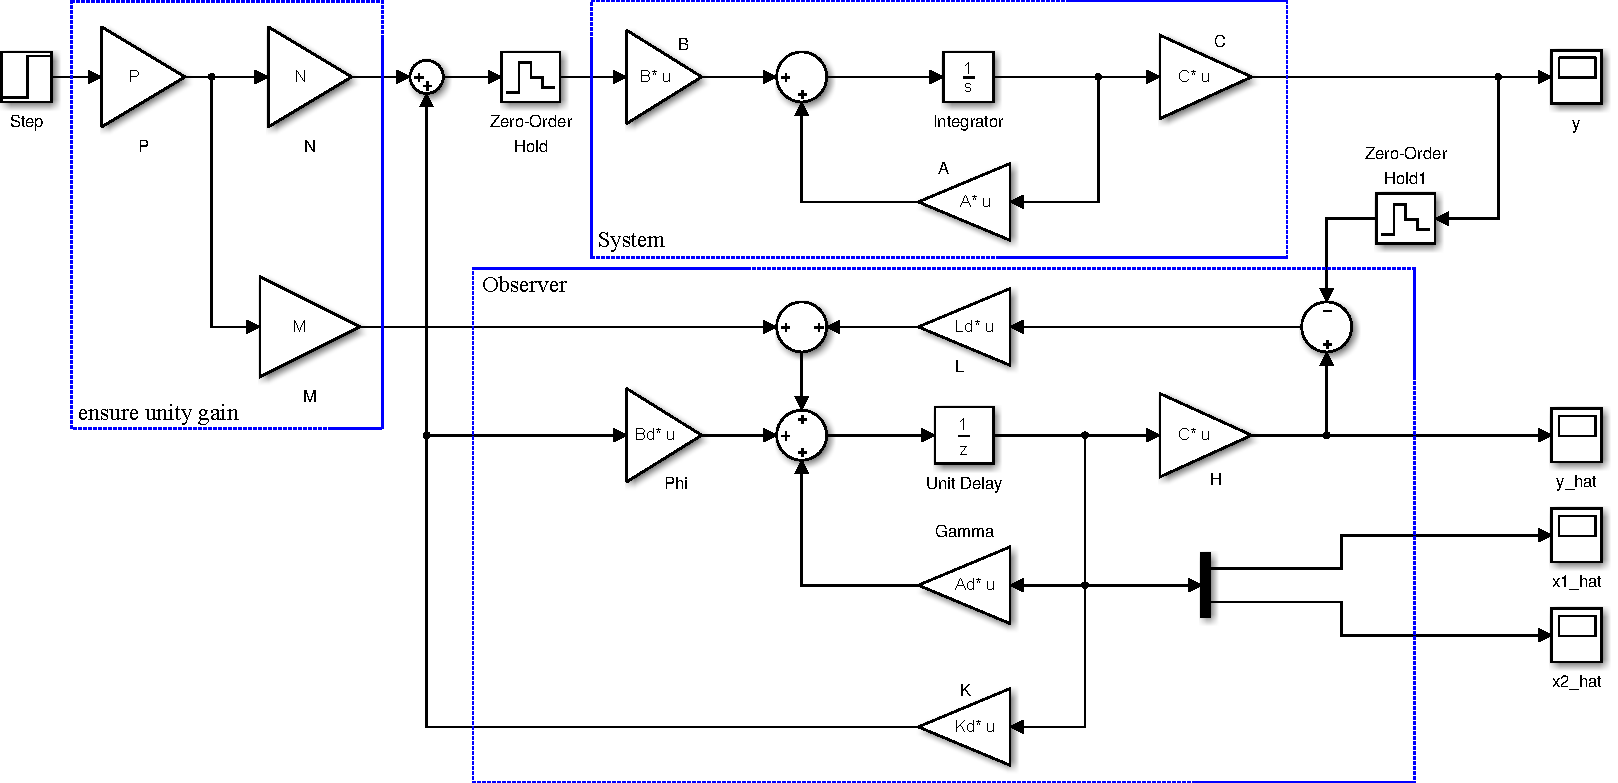
\includegraphics[scale=0.6]{observer_2_order.pdf}
	\caption{Simulink implementation of the discrete observer.}
	\label{fig:simulink_observer}
\end{figure}
The augmented (discrete) system with $\mathbf{x}_\text{augmented}\in\mathbb{R}^4$ is formulated as:
\begin{flalign*}
\begin{bmatrix}
\mathbf{x}(k+1) \\
\hat{\mathbf{x}}(k+1)
\end{bmatrix} &= \underbrace{\begin{bmatrix}
\boldsymbol\Gamma & \boldsymbol\Phi \mathbf{K}_d \\
\mathbf{L}_d \mathbf{C} & \boldsymbol\Gamma + \boldsymbol\Phi \mathbf{K}_d + \mathbf{L}_d \mathbf{C} 
\end{bmatrix} }_{\boldsymbol\Gamma_{cl}}\begin{bmatrix}
\mathbf{x}(k) \\ \hat{\mathbf{x}}(k)
\end{bmatrix} + \underbrace{\begin{bmatrix}
\boldsymbol\Phi \mathbf{N} \\ \mathbf{M}
\end{bmatrix}}_{\boldsymbol\Phi_{cl}} x_\text{ref} \\
\mathbf{y}(k) &= \underbrace{\begin{bmatrix}
\mathbf{C} & 0 & 0
\end{bmatrix}}_{\mathbf{C}_{cl}}\begin{bmatrix}
\mathbf{x}(k) \\ \hat{\mathbf{x}}(k)
\end{bmatrix}
\end{flalign*}
The discrete matrices $\boldsymbol\Gamma$ and $\boldsymbol\Phi$ can be found as \citep{bib:discrete_sampling}:
\begin{flalign}
\boldsymbol\Gamma &= \text{expm} (\mathbf{A}\, T_s) = \begin{bmatrix}
0.986 & 0.009 \\
-2.623 & 0.817
\end{bmatrix} \label{eq:Gamma_2}  \\
 \boldsymbol\Phi &= \int_0^{T_s}  \text{expm} (\mathbf{A}\, \mu) \, d \mu \cdot\mathbf{B} = \begin{bmatrix}
0.014 \\
2.623 
\end{bmatrix} \label{eq:Phi_2} 
\end{flalign}
\begin{tabular}{rl} 
where  &  \\
\text{expm}& is the matrix exponential \\
$T_s$&  is the sampling time, $T_s=100\,$ms\\
\end{tabular}\\

The sampling time $T_s$ is according to Assistant Engineer Simon Jensen limited to 100\,Hz caused by the TCP/IP communication channel between ROS and the underlying hardware as seen in \autoref{fig:overview}.

The feedback matrix and  the observer gain can now be found. They will again be calculated in MATLAB, as the design procedure follow the exact same as in \autoref{sec:K_Nbar_1D_1storder}. The poles ($p_i$) will be placed from the below considerations:
\vspace{-2mm}
\begin{itemize}
	\itemsep-0.5mm
\item No overshoot in the closed loop step response, i.e. Im($p_i)=0$.
\item Asymptotic stability, i.e. $|p_i| < 1 $
\item Slow closed loop step response
\item Positive feedback, i.e. the controller and observer gains must be negative
\item An observer significantly faster than the closed loop system $\Gamma + \Phi \mathbf{K}_d$
\end{itemize}
\vspace{-5mm}
\begin{flalign}
\mathbf{K}_d &= -\texttt{acker}\left( \Gamma,\Phi,\begin{bmatrix}
0.5 & 0.35
\end{bmatrix} \right) = \begin{bmatrix}
 -11.360 & -0.305
 \end{bmatrix} \label{eq:Kd_2} \\
 \mathbf{L}_d &= -\texttt{acker}\left( \Gamma^T,\mathbf{C}^T,\begin{bmatrix}
0.01 & 0.02
\end{bmatrix} \right) = \begin{bmatrix}
  -1.773 \\
 -68.184
 \end{bmatrix} \label{eq:Ld_2}
\end{flalign}
\vspace{-5mm}

The matrix $\mathbf{M}$ introduces zeros in the closed loop transfer function  $\mathbf{y}(k)/x_\text{ref}$. These can be eliminated by designing the zeros close to the cut-off frequency, i.e the characteristic polynomial of the matrix $\Gamma_{za}+\tilde{\mathbf{M}}\mathbf{C}_{za}$ has zeros close to the cut-off frequency, where $\Gamma_{za}=\Gamma+\Phi \mathbf{K}_d + \mathbf{L}_d \mathbf{C}$ and $\mathbf{C}_{za}=-\mathbf{K}_d$ \citep{bib:Nbar}. The MATLAB function  \texttt{acker} can again be used:
\vspace{-2mm}
\begin{flalign*}
\tilde{\mathbf{M}} = - \texttt{acker}\left( \mathbf{A}_{za}^T, \Phi_{za}^T, \begin{bmatrix}
0.01 & 0.02
\end{bmatrix} \right) = \begin{bmatrix}
  0.014 \\
   2.623
   \end{bmatrix}
\end{flalign*}
\vspace{-2mm}
To ensure unity gain, the $\mathbf{N}$ matrix can be computed as \citep{bib:Nbar}:
\vspace{-0.2cm}
\begin{flalign}
\mathbf{N} &= - \left( \mathbf{C}_{cl} \Gamma_{cl}^{-1} \tilde{\Phi}_{cl} \right)^{-1} \kk \text{where} \mm \tilde{\Phi} = \begin{bmatrix}
\Phi \\ \tilde{M}
\end{bmatrix} \nonumber \\
\mathbf{N} &= 13.739 \label{eq:N_2}
\end{flalign}
\vspace{-0.2cm}
The other matrix $\mathbf{M}$ ensuring unity gain, can now be calculated as \citep{bib:Nbar}:
\begin{flalign}
\mathbf{M} = \tilde{\mathbf{M}}\mathbf{N} = \begin{bmatrix}
 0.186 \\
  36.040
\end{bmatrix}
\label{eq:M_2}
\end{flalign}
\vspace{-0.2cm}
Thereby, all unknowns from \autoref{eq:observer} is calculated.

\begin{recap}[Control Law for Second Order Approximation]
	The complete controller based on the second order system approximation is now designed as:
\begin{flalign*}
&\textbf{1.}  \phantom{\mathbf{u}(k)}\hat{\mathbf{x}}(k+1) = \Gamma \hat{\mathbf{x}}(k) + \Phi \mathbf{K}_d \hat{\mathbf{x}}(k) + \mathbf{L}_d (\mathbf{C}\hat{\mathbf{x}}(k)-\mathbf{y}(k) ) + \mathbf{M} x_\text{ref} \\
&\textbf{2.} \phantom{\hat{\mathbf{x}}(k+1)}\mathbf{u}(k) = \sigma(\mathbf{x})k_0(\hat{\mathbf{x}})+(1-\sigma(\mathbf{x}))(\mathbf{N} \cdot x_\text{ref}-\mathbf{K}_d\hat{\mathbf{x}}(k))
\end{flalign*}
\begin{tabular}{rl} 
where  &  \\
$\sigma(\mathbf{x})$ & is computed from \autoref{eq:smoothness} with $\epsilon$ from in \ref{eq:epsilon_2} and the \gls{cbf} found in \ref{eq:cbf2}  \\
$k_0(\mathbf{x})$ & is computed from \autoref{eq:control_law} with Lie derivatives from \ref{eq:LgB_2} and \ref{eq:LfB_2}  \\
$\Gamma$ & is found in \autoref{eq:Gamma_2} \\
$\Phi$ & is found in \autoref{eq:Phi_2}  \\
$\mathbf{N}$ & is found in \autoref{eq:N_2}  \\
$\mathbf{M}$ & is found in \autoref{eq:M_2} \\
$\mathbf{L}_d$& is found in \autoref{eq:Ld_2} \\
$\mathbf{K}_d$ & is found in \autoref{eq:Kd_2} \\
$\mathbf{C}$ & is found in \autoref{eq:system:2}
\end{tabular}
\vspace*{-5mm}
\end{recap}
This completes the control design. The implementation constitutes both a MATLAB simulation and an actual implementation on the Da Vinci robot in \gls{ros}. The MATLAB implementation is outlined first. 
\vspace{-0.3cm}
\section{MATLAB Implementation and Results}\label{sec:matlab-results-slide-safety}
\vspace{-0.2cm}
The results shown in this section are based on the implemented controller found in \autoref{app:slide_implement_1} and in \autoref{app:cd} under the path \texttt{matlab\_scripts\_slide\_controller\_slide\_controller.m}. All plots are made with the following characteristics:
\begin{itemize}
\item The sampling rate is tested with both $f_s = 2\,$kHz (expected sampling rate in the long run) and $f_s = 100\,$Hz (current limitation of the sample rate caused by the TCP/IP communication channel).
\item The control signal is limited to $\pm 0.1$\,m (actual limit for slide movement).
\item The velocity is limited to $\pm$1\,m/s (actual limit for slide movement).
\item The forward euler method is used to extrapolate the states.
\item The design parameter $\kappa$ from \autoref{eq:control_law} is set to $\kappa=1$ (neutral).
\item The simulation time is 5\,s. Various setpoints ought to indicate the behaviour in different regions.
\end{itemize}
The \texttt{model} variable in the first line in \autoref{app:slide_implement_1} is set to the number 1 for the first order model and 2 for the second order model. 
\vspace{-0.3cm}
\subsection{MATLAB Results based on First Order Model}\label{subsec:matlab-results-1order}
The state trajectory composing slide position is plotted in \autoref{fig:trajectory1}
%
\begin{figure}[H]
%\hspace*{-10mm}
\subbottom[State trajectory with $f_s = 2\text{kHz}$.]{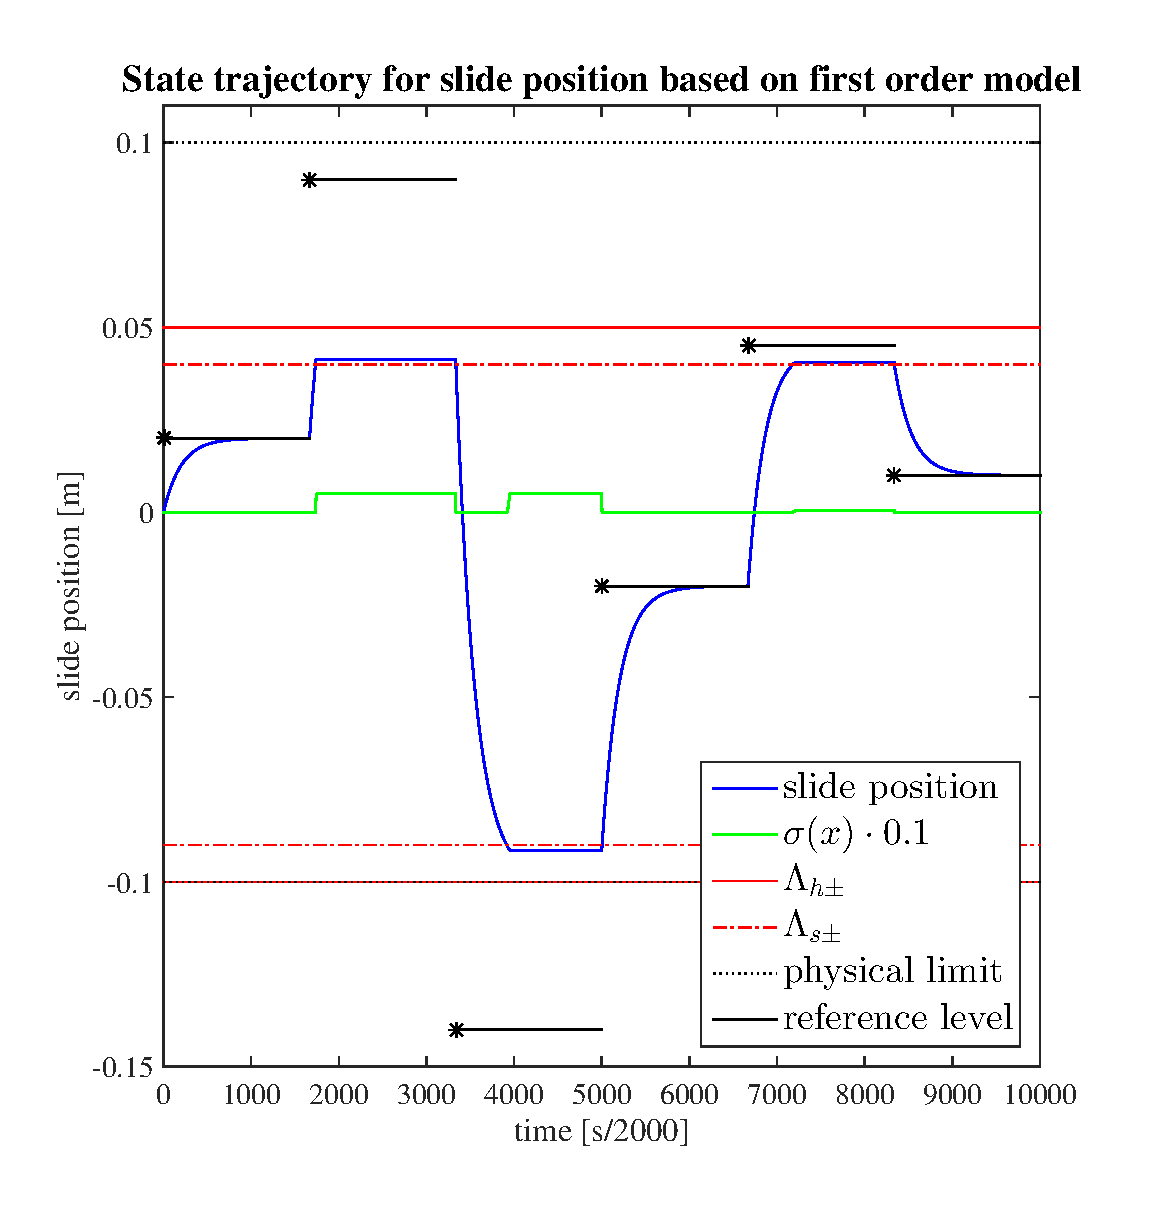
\includegraphics[width=0.5\textwidth]{trajectory_2kHz.eps}\label{fig:2khz_1}}%
\subbottom[State trajectory with $f_s = 100\text{Hz}$.]{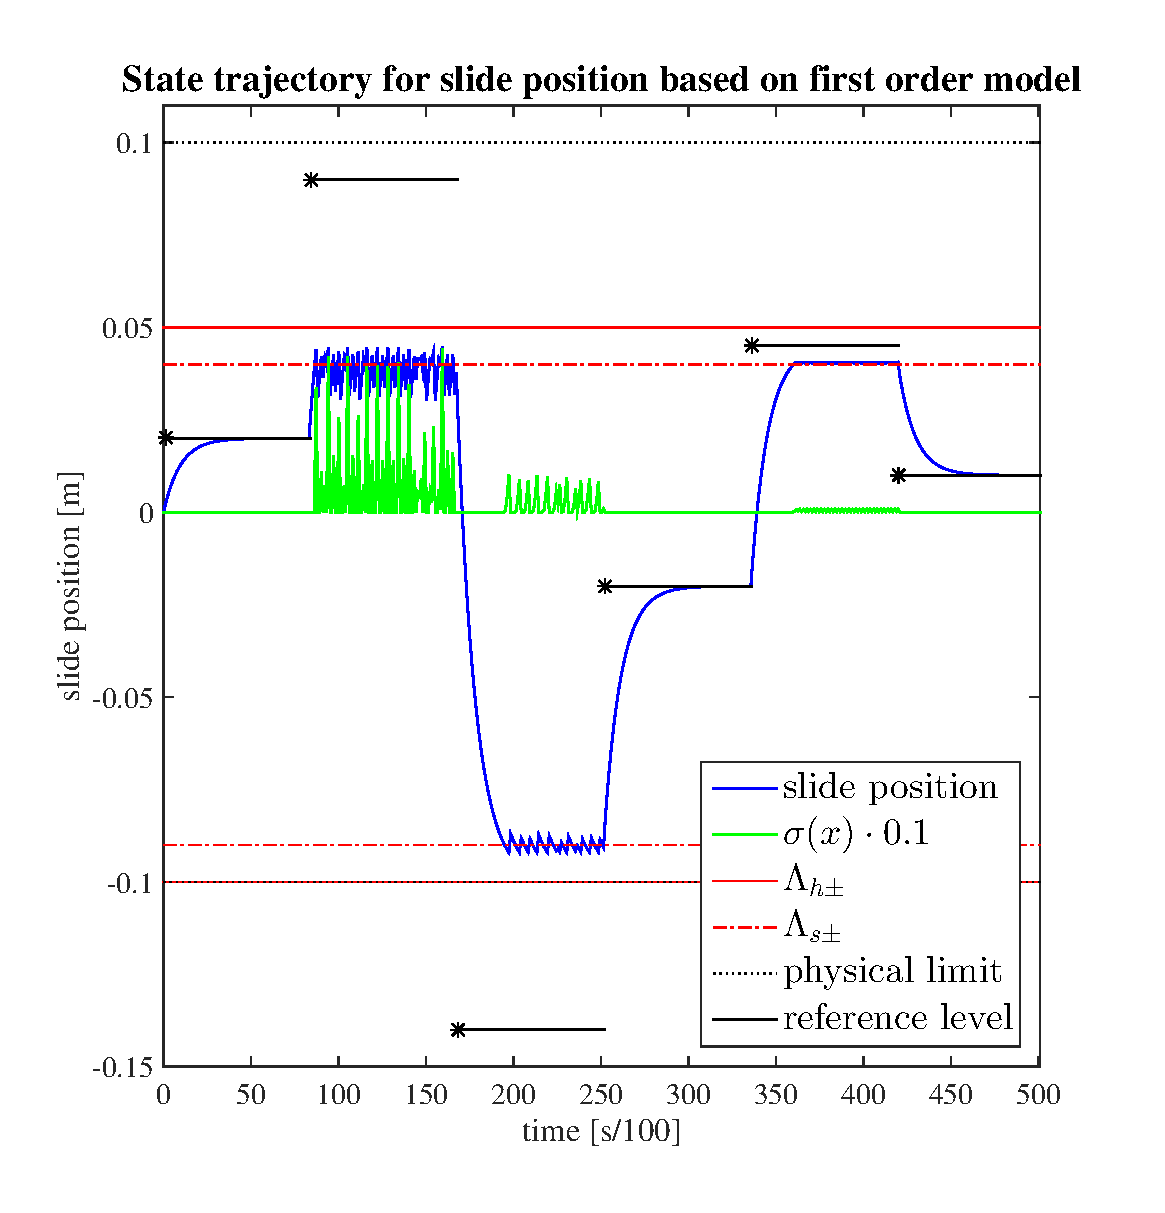
\includegraphics[width=0.5\textwidth]{trajectory_100Hz.eps}\label{fig:100hz_1}}%
\caption{State trajectory for slide position for $\kappa=1$. MATLAB implementation can be found in \autoref{app:slide_implement_1}. The plot is based on forward euler. It is seen how the correct position is obtained in the interval $[\Lambda_{s-}:\Lambda_{s+}$]. When setpoints are given outside the safe area, the safety controller ensures that the hard boundaries $\Lambda_{h+}$ and $\Lambda_{h-}$ are not exceeded at any time and that the position finds its equilibrium at a state determined by the linear combination of the two controllers.}
\label{fig:trajectory1}
\end{figure}
%
%
%\begin{figure}[H]
%	\center
%		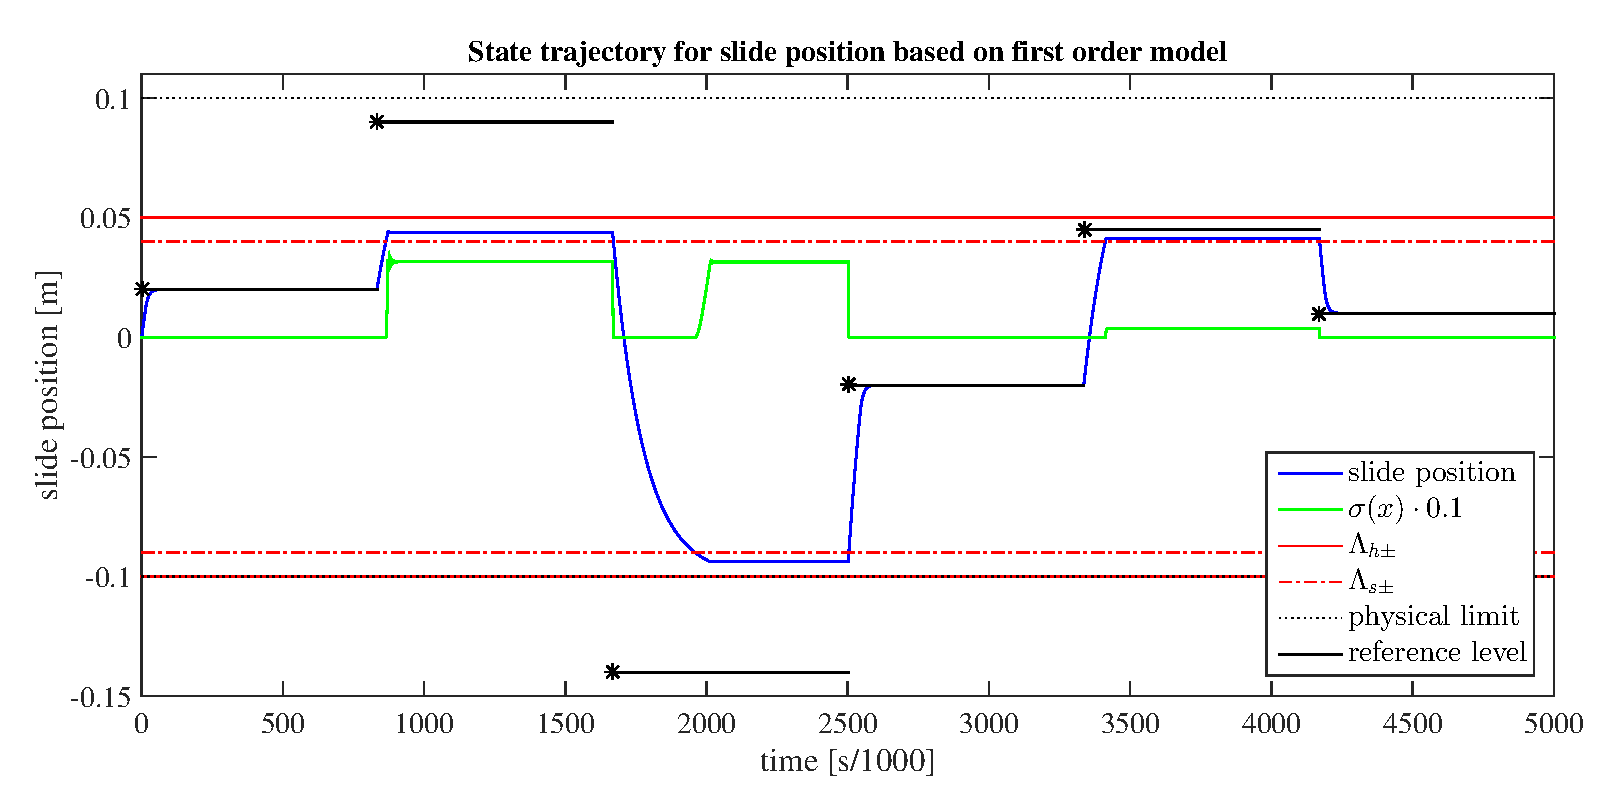
\includegraphics[scale=0.6]{trajectory_slide.eps}
%	\caption{State trajectory for slide position for $\kappa=1$. MATLAB implementation can be found in \autoref{app:slide_implement_1}. The plot is based on forward euler with a sampling rate of $1\,$kHz. It is seen how the correct position is obtained in the interval $[\Lambda_{s-}:\Lambda_{s+}$]. When setpoints are given outside the safe area, the safety controller ensures that the hard boundaries $\Lambda_{h+}$ and $\Lambda_{h-}$ are not exceeded at any time and that the position finds its equilibrium at some arbitrary state.}
%	\label{fig:trajectory1}
%\end{figure}
Varying $\kappa$ increases the aggressivity of the safety controller and can create fluctuations in the transition area if the sampling rate is too low. Likewise $\sigma(x)$ will fluctuate along with an increased $\kappa$. One must be careful when increasing $\kappa$ when the sampling rate is relatively low. %The effect of increasing $\kappa$ ten times is shown in \autoref{fig:trajectory2}.
%\begin{figure}[H]
%	\center
%		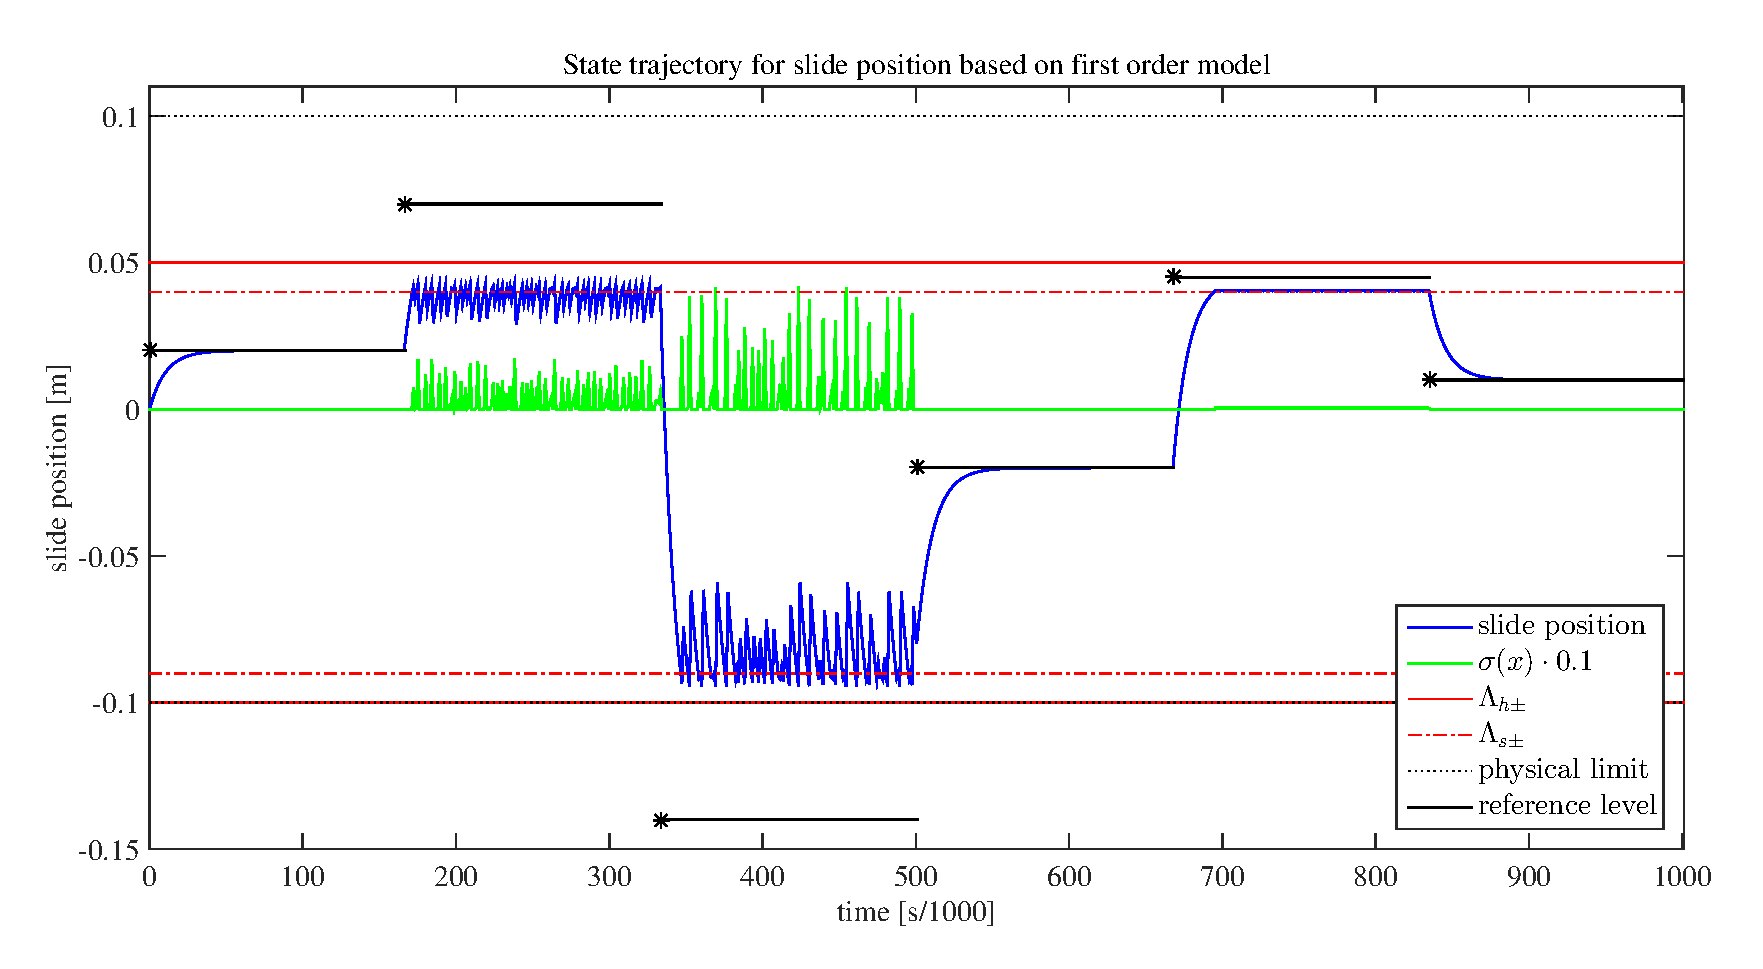
\includegraphics[scale=0.5]{trajectory_slide_kappa_10.eps}
%	\caption{State trajectory for slide position for $\kappa=10$ based on same control law and model as \autoref{fig:trajectory1}. It is seen how the safety controller is more aggressive.}
%	\label{fig:trajectory2}
%\end{figure}

To verify that \autoref{req2} is fulfilled in the simulation, the Lie derivatives are plotted in \autoref{fig:lie1}.
\begin{figure}[H]
	\center
		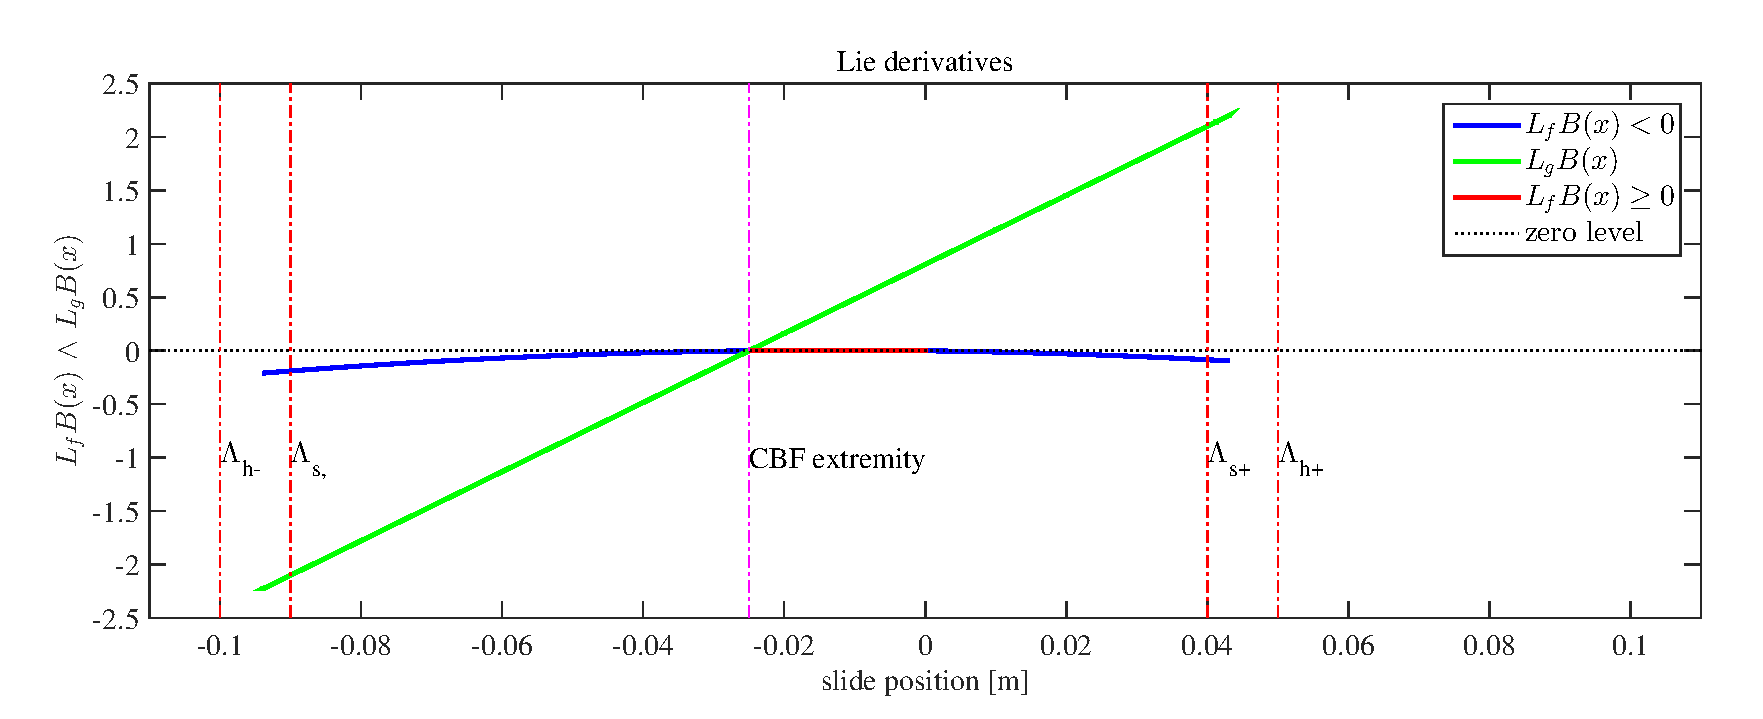
\includegraphics[width=1\textwidth]{Lie_slide_1d.eps}
	\caption{Lie derivatives of the CBF along the vector fields $f(x) = Ax$ and $g(x)=B$. It is seen that $L_gfB(x) \neq 0 \,\, \forall x \neq \frac{-b}{2a}$ which essentially fulfils \autoref{req2}.}
	\label{fig:lie1}
\end{figure}
It is from \autoref{fig:lie1} seen that $L_gB(x) \neq 0 \,\, \forall x \neq -b/(2a)$ which essentially fulfils \autoref{req2}. Indeed, even if the entire range $[\Lambda_{h-}:\Lambda_{h+}]$ belongs to $\mathcal{X}$, the chosen CBF would have been valid because the only place where $L_gB(x) = 0$ is at the critical point. Note also that the Lie derivatives are independent of the scalar $\kappa$.
%For the record, the control signal is plotted in \autoref{fig:control1}.
%\begin{figure}[H]
%	\center
%		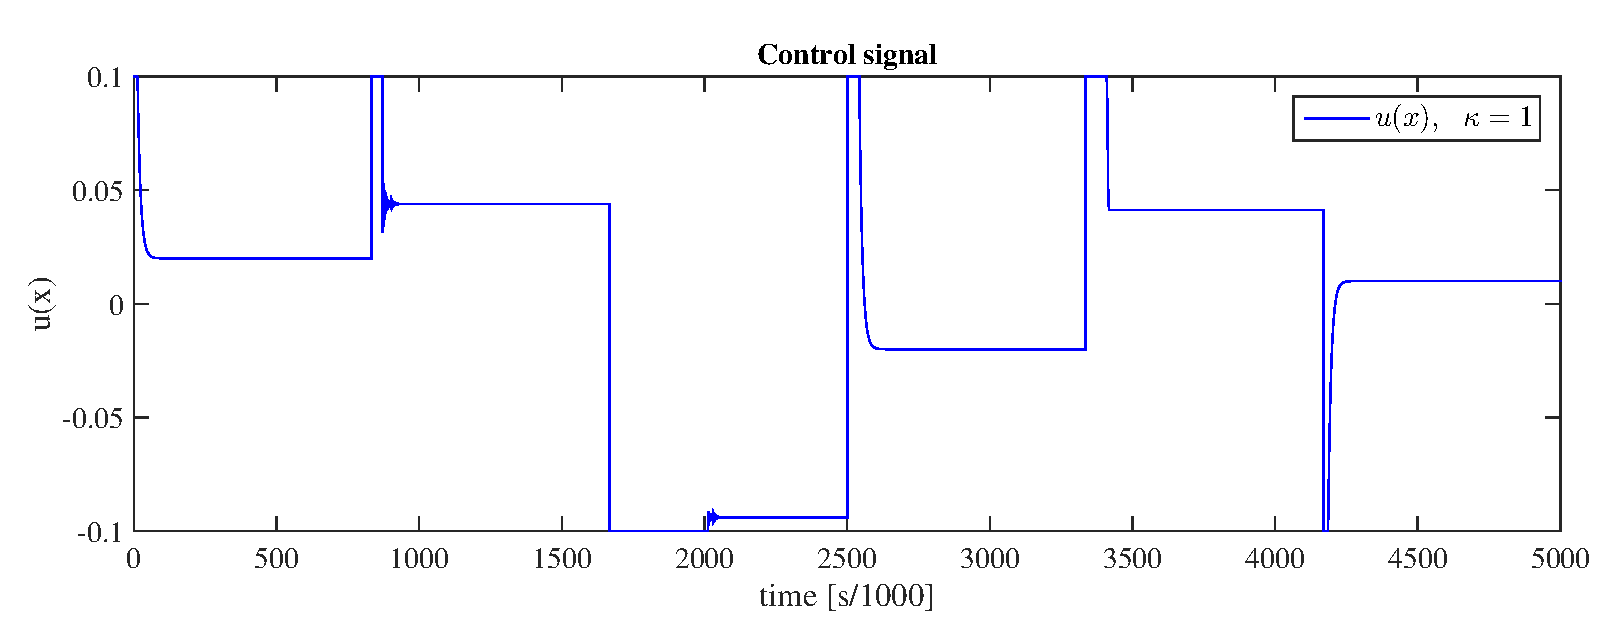
\includegraphics[scale=0.55]{control_slide_1.eps}
%	\caption{Control signal for $\kappa=1$. It is seen how the controller counteracts the large difference in setpoints given and in that way ensures safety. It is seen that when the absolute value of the setpoints are increased then $u(x)$ increases accordingly. The plot is ideal as no saturation constraints are given.}
%	\label{fig:control1}
%\end{figure}
%It is seen from \autoref{fig:control1} how the control signal reacts instantaneously and quite aggressive when $\Lambda_s$ is exceeded to counteract the large difference in setpoints given. It is also noted how the controller eventually settles smootly even when setpoints are given in the interval $[-\infty:\Lambda_{s-}]$ and $[\Lambda_{s+}:\infty]$. However, as the setpoints approaches $\pm \infty$, the sampling rate must also converge towards infinity. This is obviously not a realistic scenario as the slide movement is physically constrained.
\vspace{-0.3cm}
\subsection{MATLAB Results based on Second Order Model}\label{subsec:matlab-resutls-2-order}
\vspace{-0.2cm}
The state trajectory composing slide position based on the second order model is shown in \autoref{fig:traject2}.
\begin{figure}[H]
%\hspace*{-10mm}
\subbottom[State trajectory with $f_s = 2\text{kHz}$.]{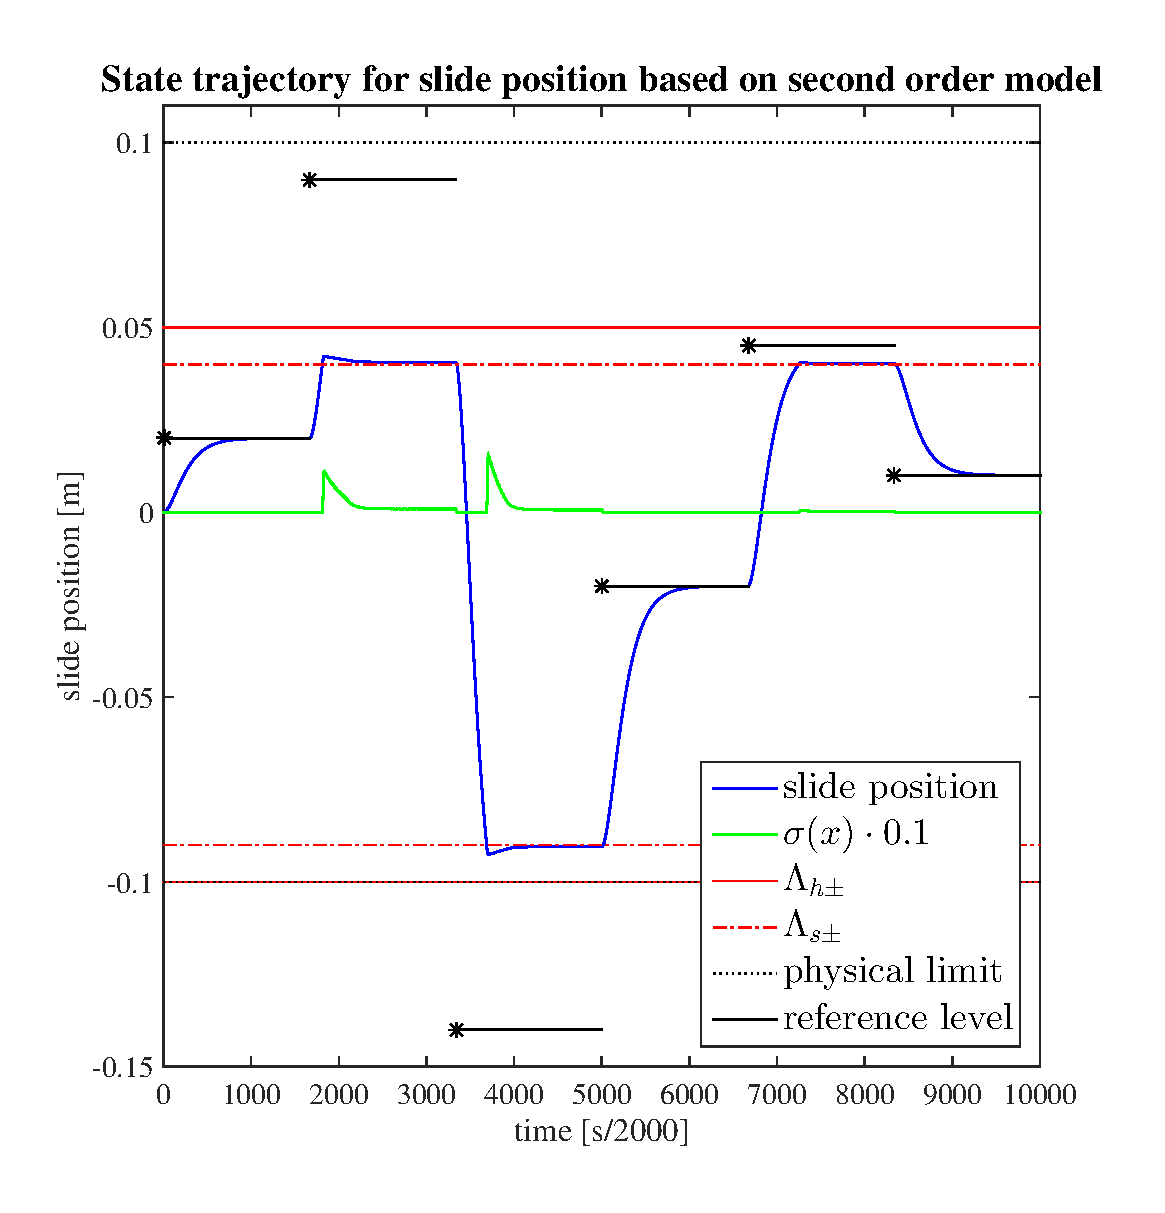
\includegraphics[width=0.5\textwidth]{trajectory_2_2kHz.eps}\label{fig:2khz_2}}%
\subbottom[State trajectory with $f_s = 100\text{Hz}$.]{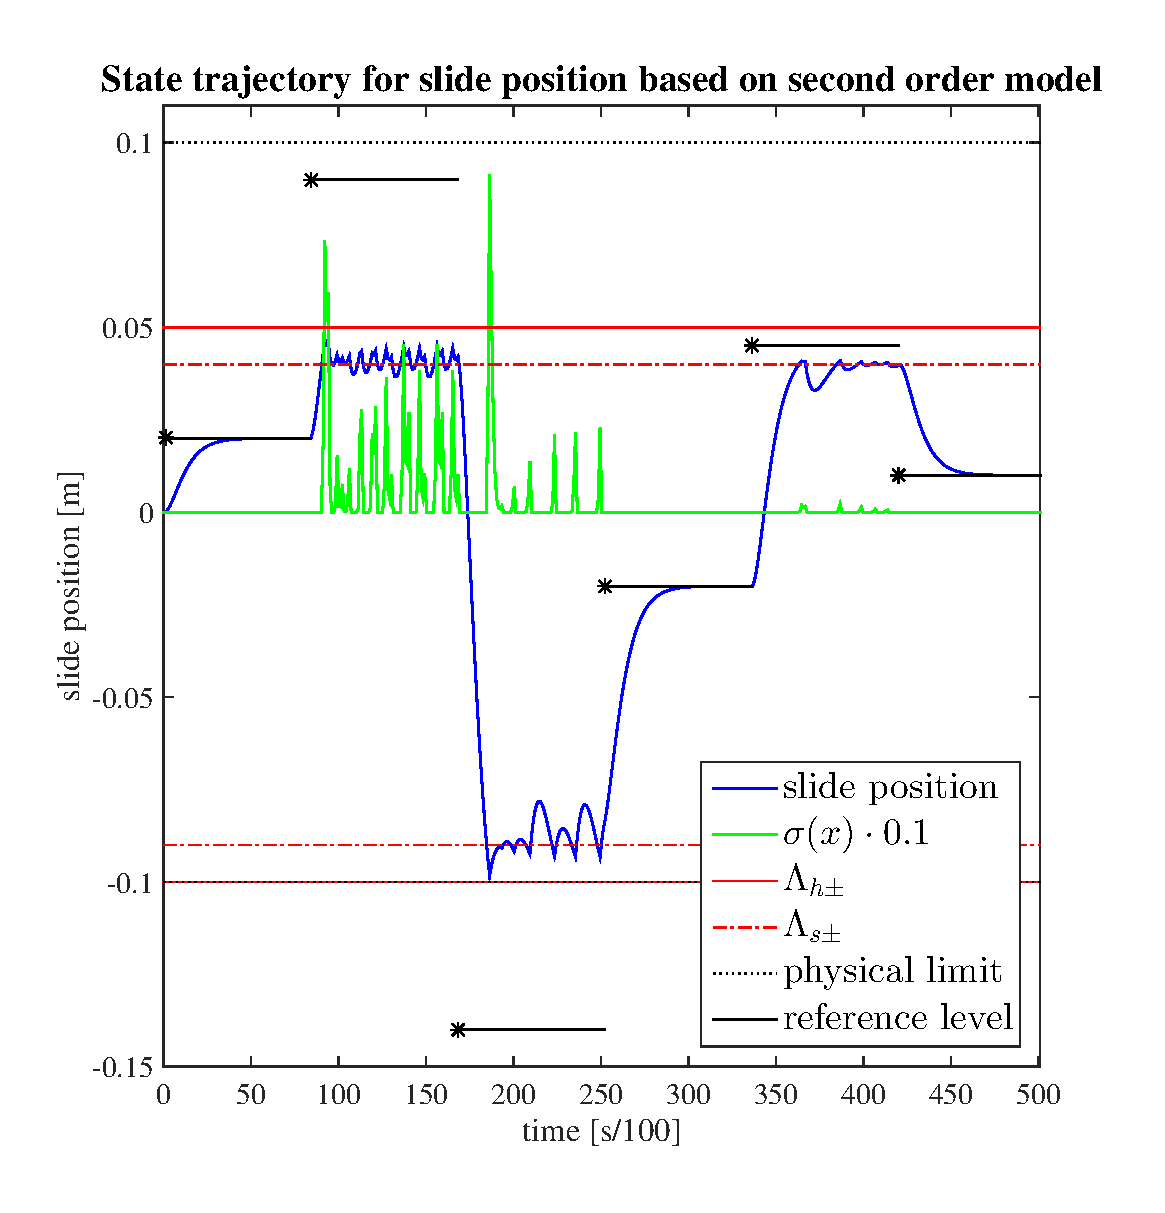
\includegraphics[width=0.5\textwidth]{trajectory_2_100Hz.eps}\label{fig:100hz_2}}%
\caption{State trajectory for position based on second order system approximation. It is seen how the boundaries are respected at all time regardless of irresponsible/unsafe setpoints. It is seen how $\sigma(x)$ 	increases when setpoints are given in the unsafe area. AS a result, the control law is a linear combination of the safety controller $u(x) = k_0(x)$ and the linear controller by pole-placement $\tilde{u}(x)$..}
\label{fig:traject2}
\end{figure}
%
%
%
%
%\begin{figure}[H]
%	\center
%		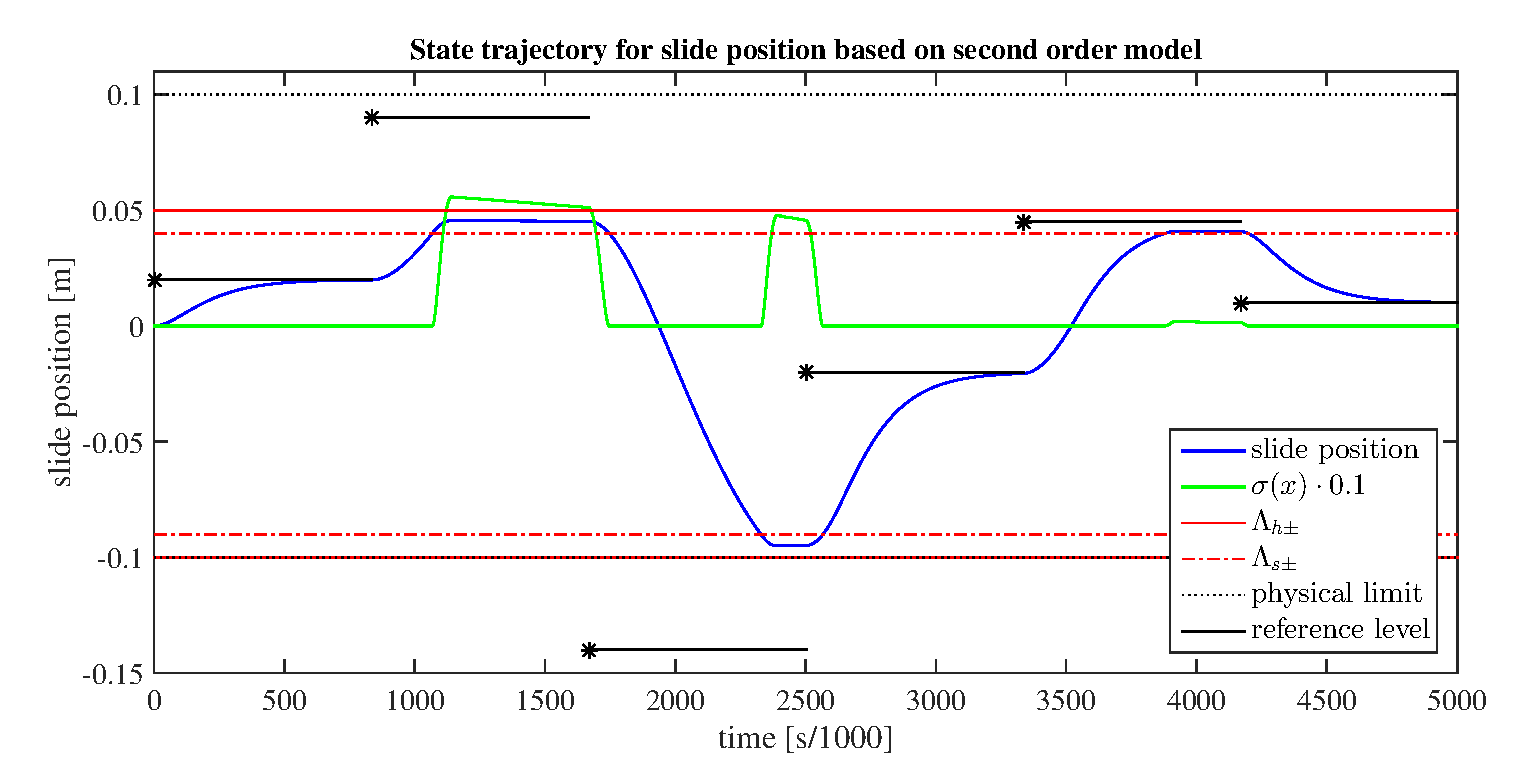
\includegraphics[scale=0.6]{trajectory_slide_second_order_model_kappa_1.eps}
%	\caption{State trajectory for position based on second order system approximation. It is seen how the boundaries are respected at all time regardless of irresponsible/unsafe setpoints. It is seen how $\sigma(x)$ 	increases when setpoints are given in the unsafe area. AS a result, the control law is a linear combination of the safety controller $u(x) = k_0(x)$ and the linear controller by pole-placement $\tilde{u}(x)$.}
%	\label{fig:traject2}
%\end{figure}
The state trajectory shown in \autoref{fig:traject2} verifies that the slide position does not exceed its limits even when setpoints are given outside the safe region.

The Lie derivatives are plotted in \autoref{fig:lie2}.
\begin{figure}[H]
	\center
		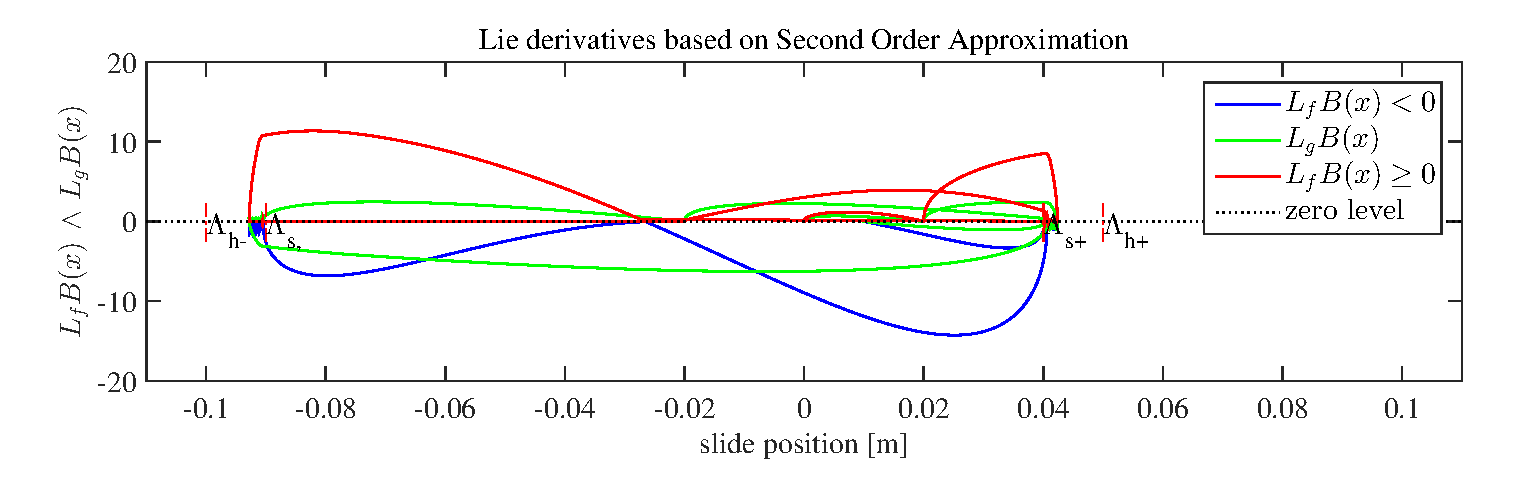
\includegraphics[width=1\textwidth]{Lie_slide_2d.eps}
	\caption{Lie derivatives. It is seen how $L_gB(x_1,x_2) = 0 \wedge L_fB(x_1,x_2) = 0$ at the same time which in general is critical but accepted in this specific case as it is caused by $x_2=0$ which implies $u(x)=0 \,\,\, \Rightarrow \,\,\, x_1 \rightarrow 0$ which is safe.}
	\label{fig:lie2}
\end{figure}
%The constrained control signal is plotted in \autoref{fig:control2}
%\begin{figure}[H]
%	\center
%		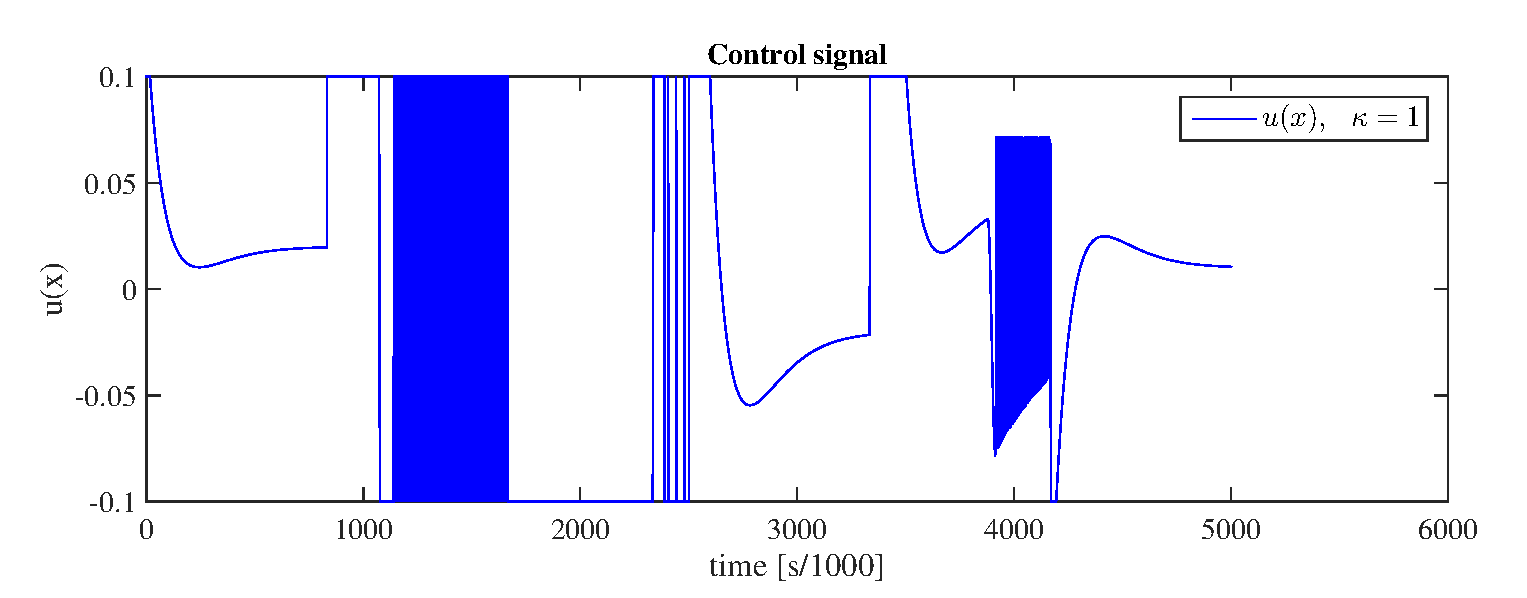
\includegraphics[scale=0.5]{control_signal_2.eps}
%	\caption{Control signal. It is seen how the it fluctuates heavily when $x_1 \in \Delta_t$ due to the position gradient.}
%	\label{fig:control2}
%\end{figure}
%It is from \autoref{fig:control2} noted how the control signal fluctuates heavily. This is because the position gradient (the velocity) changes sign constantly in the unsafe region as the trajectory seeks to go either one or the other way due to the safety controller and the setpoint given outside the safe region.
\subsection{Observer Verification}
The observer developed in \autoref{sec:K_Nbar_1D_2ndorder} will be verified with a step input at 1\,cm. The estimated position and velocity is plotted with the success criteria that $\hat{x}_1 = x_\text{ref}$ for $t \rightarrow \infty$ and no overshoot in the position occurs. The velocity must stay within a reasonable velocity span, i.e. below 1\,m/s when the time constant is considered. The error is defined as $\hat{y}-y$ and should obviously stay very low in steady state. The result is plotted in \autoref{fig:observerplot}.
\begin{figure}[H]
	\center
		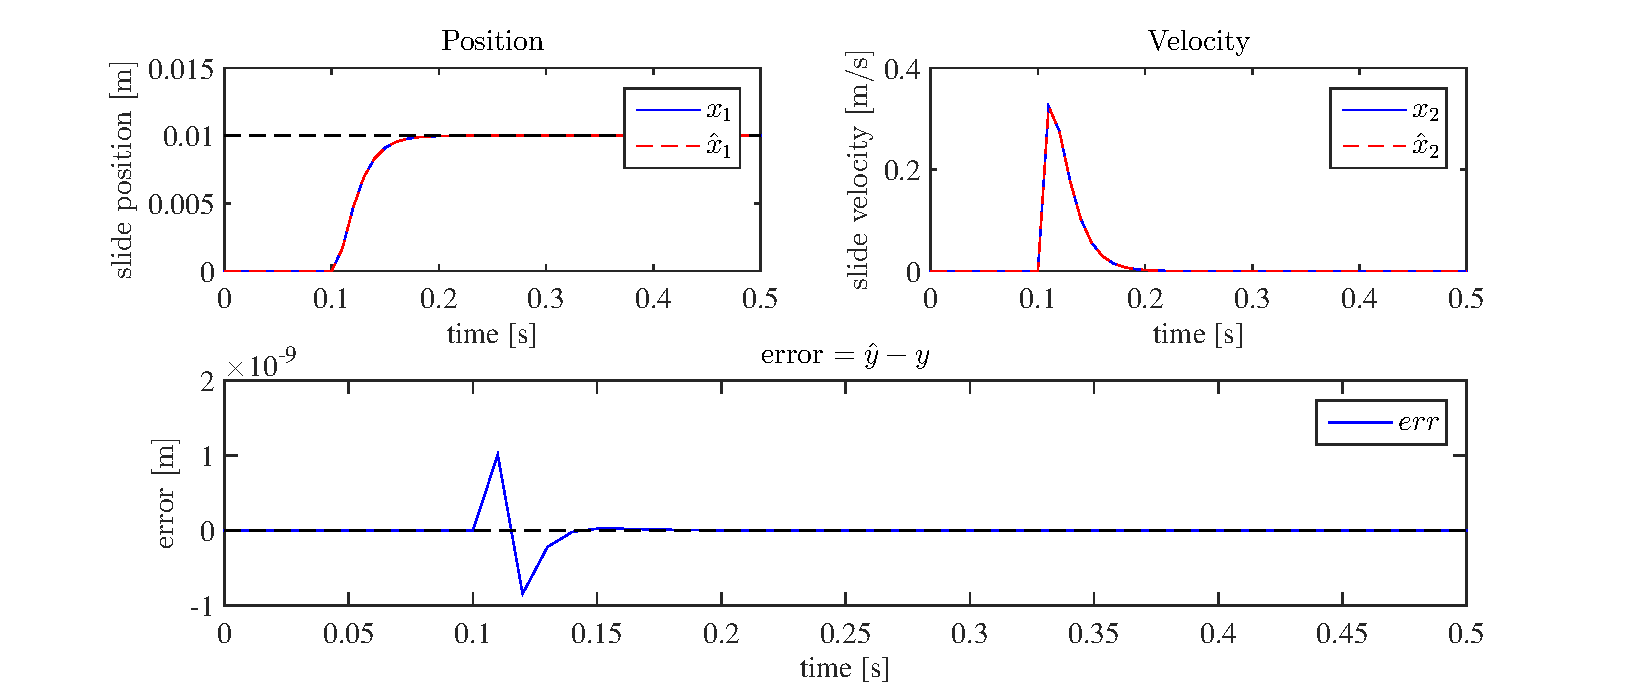
\includegraphics[width=1\textwidth]{observer_plot.eps}
	\caption{Simulation results from the simulink implementation of the observer. Plot details and simulink file can be found in \autoref{app:cd} by running \texttt{run\_observer.m} under the path \texttt{matlab\_scripts/observer/}.}
	\label{fig:observerplot}
\end{figure}
It is from \autoref{fig:observerplot} seen how the position, velocity and error all complies with the expected outcome and fulfil the requirements.

The outlined plots throughout this section concludes the MATLAB simulation. The MATLAB implementation shows the expected scenario, i.e. that the state trajectory complies with the outlined safe and unsafe regions. It shall now be seen how to implement the results on the Da Vinci robot itself.
\section{Implementation on the Da Vinci Robot}\label{sec:davinci-implementation}
The implementation constitutes the below listed bullet points:
\begin{itemize}
\item The controller will be implemented in C++. \textbf{Reason:} Along with Python, C++ is \underline{the} ROS compatible standard. The reason to use C++ over Python is to optimize speed performance. Furthermore, it is the general opinion among ROS experts (such as Postdoc Karl Damkj\ae r Hansen and others) that C++ is more useful in robot simulations and development and lastly, the already existing code at the Robotic Surgery Group - Aalborg University, is by far mostly developed in C++. However, Python as a scripting language, may be more user friendly, easier to get started with and in many cases more readable.
\item Real-time signal processing to ensure fixed sample rates. \textbf{Reason:} The observer matrices are built upon fixed sampling rates and for that reason it is crucial to comply with a fixed sample rate.
\item Algorithm development to connect these two bullet points.
\end{itemize}
The controller is implemented at the highest abstraction layer, i.e. the ROS environment depicted in \autoref{fig:overview}. While ROS runs on most Linux laptops, it is not ROS itself that put fort limitations for real time signal processing, neither is it the potentiometers that measures the angle. The bottleneck is caused by the TCP/IP communication channel which according to Assistant Engineer Simon Jensen is limited to 100\,Hz. For that reason, the maximum allowed execution time $c_{p,\text{max}}$ is:
\begin{flalign*}
c_{p,\text{max}} = \dfrac{1}{100\,\text{Hz}} = 10\,\text{ms}
\end{flalign*}
The main algorithm is depicted in \autoref{fig:slide_safery_algorithm}.
\begin{figure}[H]
	\center
		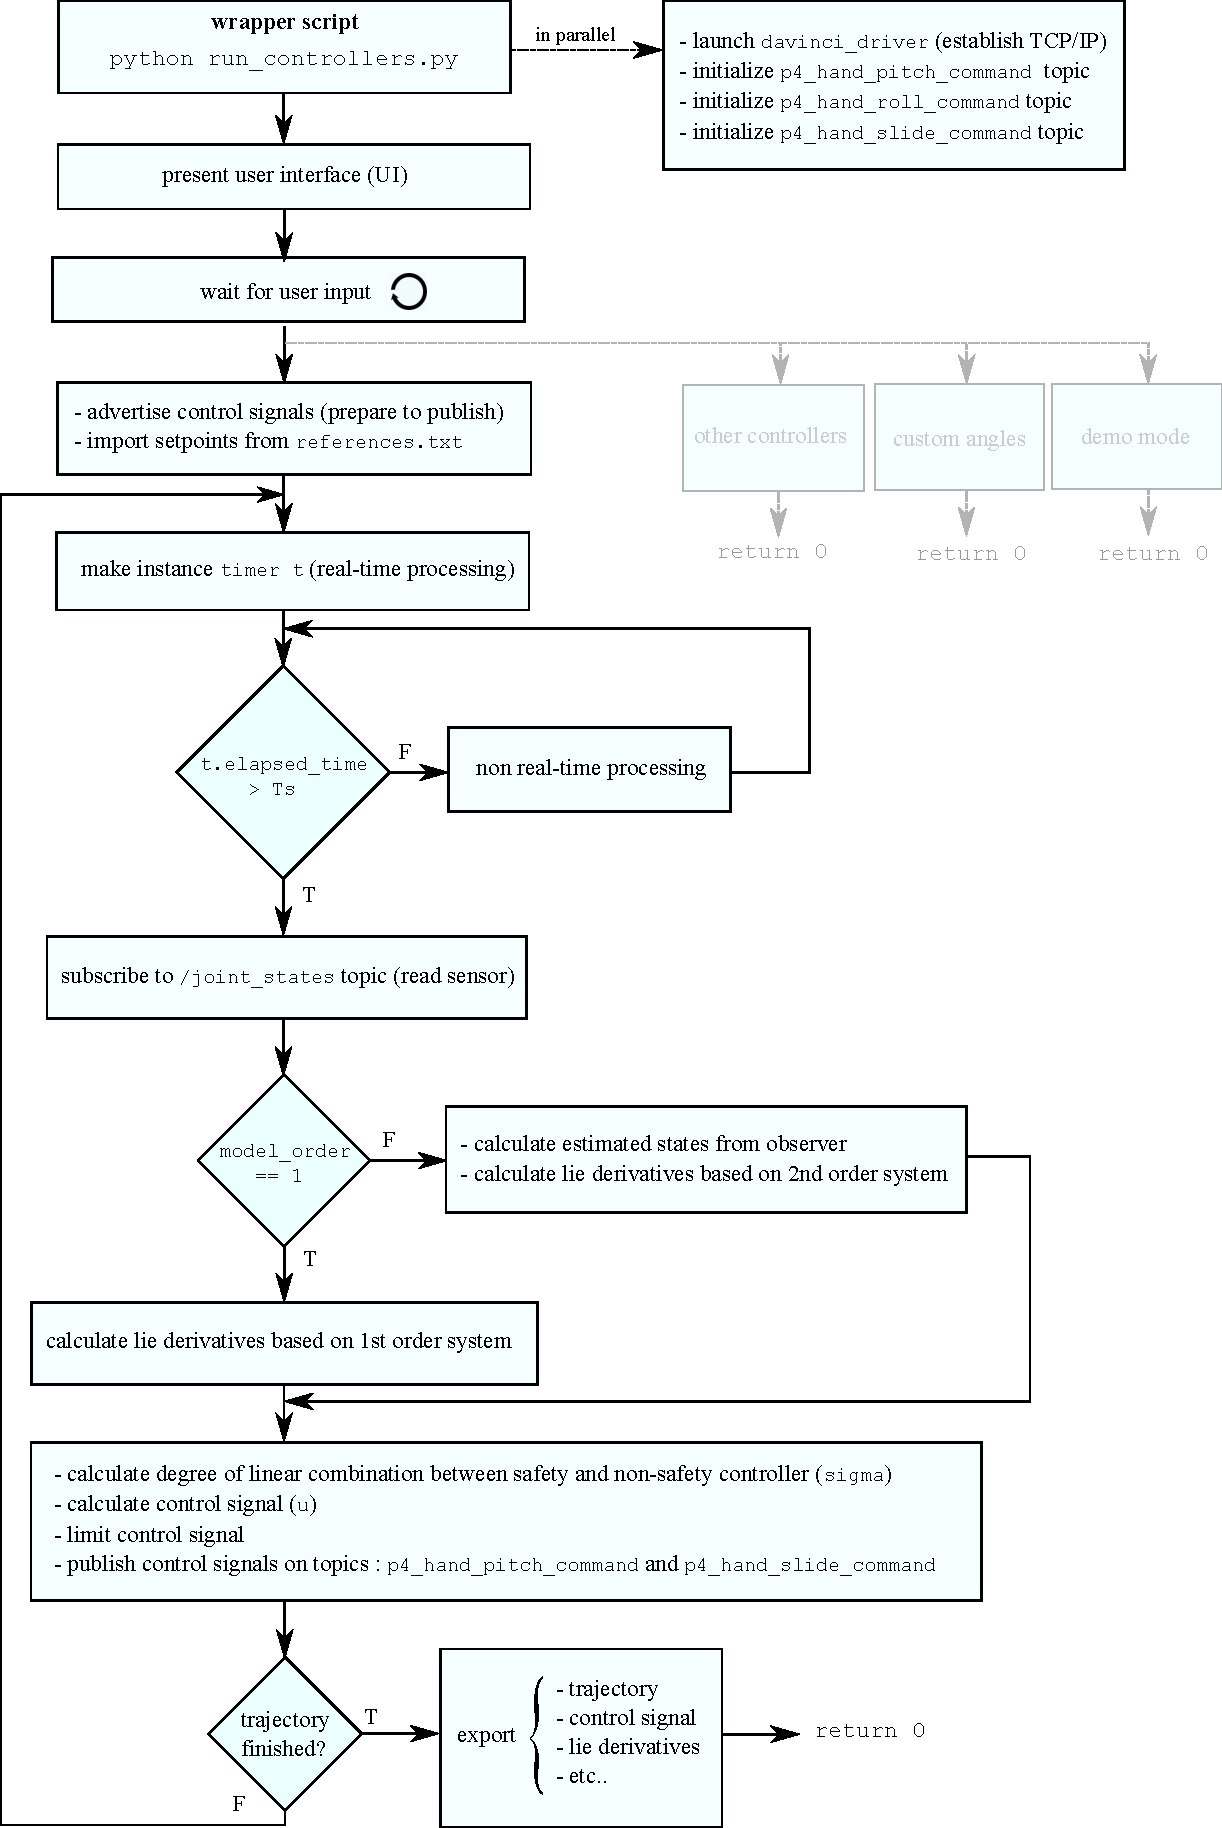
\includegraphics[scale=0.7]{flowchart_safety_controller.pdf}
	\caption{Algorithm for slide safety controller.}
	\label{fig:slide_safery_algorithm}
\end{figure}
The source code associated with the algorithm from \autoref{fig:slide_safery_algorithm} can be found in \autoref{app:slide_implement_2} and in \autoref{app:cd}. It can also be found at github at the Robotic Surgery Group - Aalborg University under the repository \texttt{gr1032} (\textit{https://github.com/AalborgUniversity-RoboticSurgeryGroup/}).
\subsection{Implementation on the Da Vinci Robot based on 1D Model}\label{subsec:implement-davinci-1d}
All plots and measurement in this subsection can be reconstructed by running the MATLAB script \texttt{plot\_data} found in \autoref{app:cd} in the folder \texttt{measurements/slide\_safety\_controller/1D\_1st\_order}. The execution time is validated first as it is essential for the controller to complete successfully. A plot measuring the execution time for each iteration is shown in \autoref{fig:exe_1}.
\begin{figure}[H]
	\center
		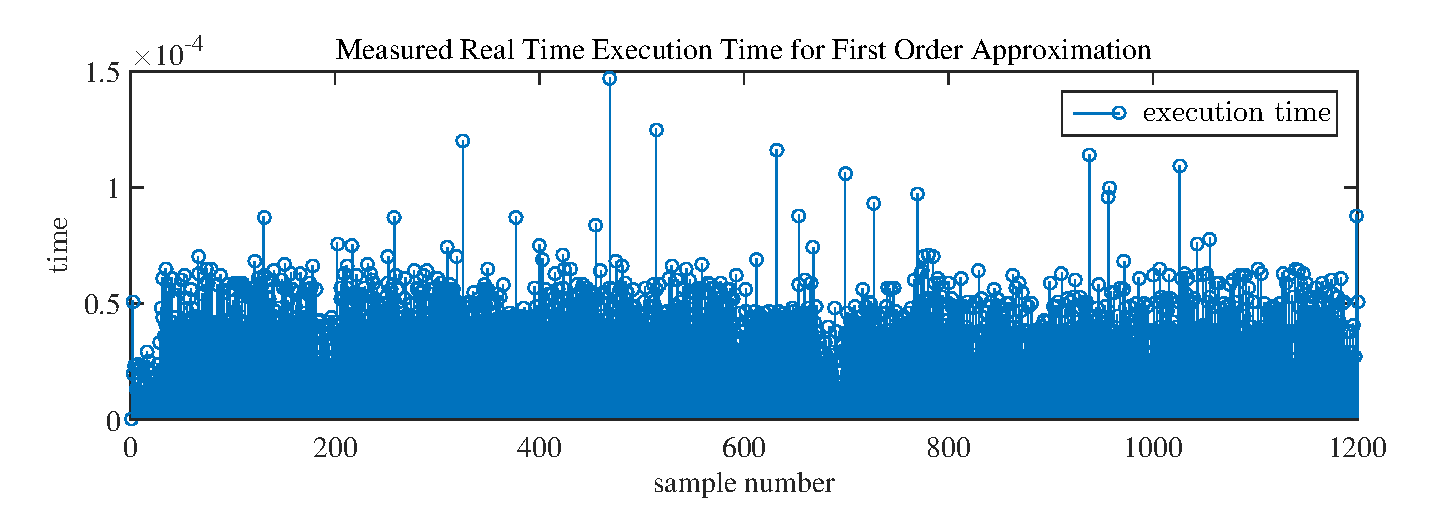
\includegraphics[scale=0.6]{execution_time_1_order.eps}
	\caption{Execution time for the first order system approximation. It is seen that the controller never exceed at computation time of 150\,$\mu$s.}
	\label{fig:exe_1}
\end{figure}
It is from \autoref{fig:exe_1} seen that $c_p < c_{p,\text{max}}$ and the real-time part is therefore verified.

The measured state trajectory is plotted in \autoref{fig:traj_meas_1}.
\begin{figure}[H]
	\center
		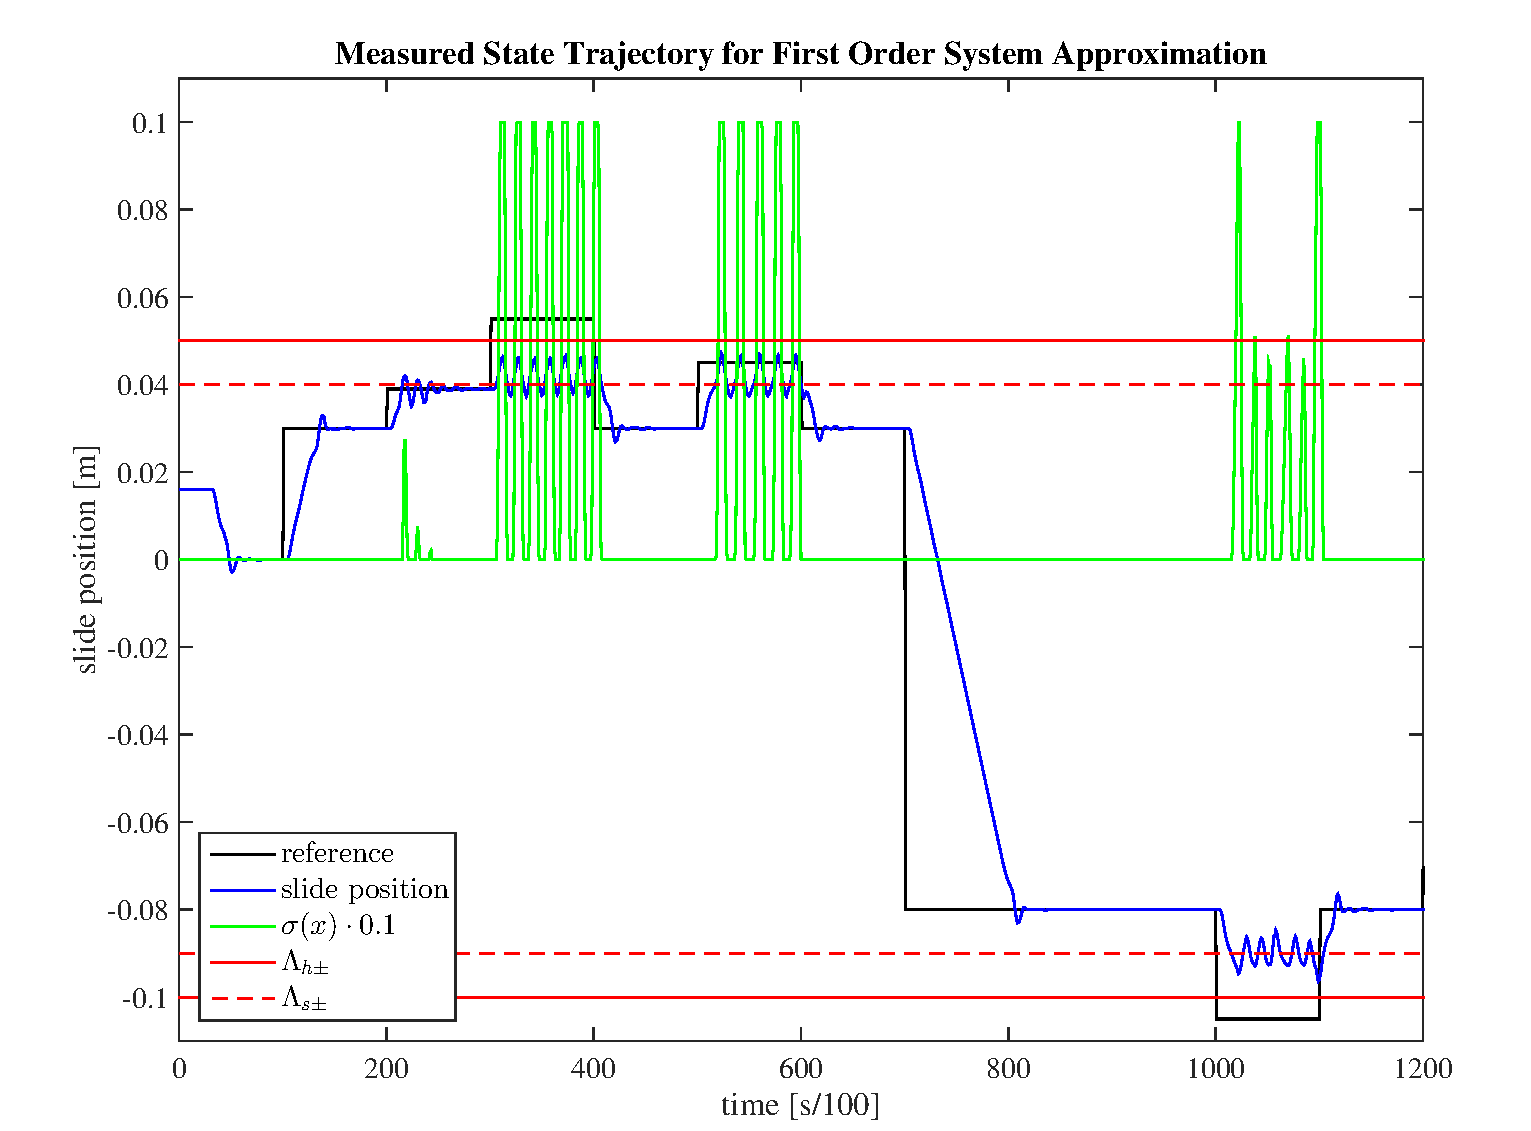
\includegraphics[scale=0.65]{trajectory_slide_meas_1.eps}
	\caption{Measured position trajectory based on the first order approximation.}
    \label{fig:traj_meas_1}
\end{figure}
It is from \autoref{fig:traj_meas_1} seen how the controller ensures that $x \in \mathcal{X}_u^c \ \ \forall \, x$. The poor system approximation is also revealed as the trajectory has an overshoot which was not included in the simulation found in \autoref{fig:trajectory1}. This is however not surprisingly as the first order approximation was created to simplify the control barrier function and to avoid the observer design as an initial approach. A consequence of the overshoot is seen when setpoints very close to $\Lambda_{s+}$ are given. The slide movement starts to oscillate which is caused by $\sigma(x)$. This is obviously not a good thing, but nevertheless the intended outcome when $x \in \mathcal{T}$. Additionally, it is seen how $\sigma(x)$ forces the position below its setpoint when $x_\text{ref} \in \mathcal{X}_u$ but allows $x_1 > x_\text{ref}$ when $x \in \mathcal{T}$. This is indeed the effect of $\sigma(x)$. It is finally seen that the safety controller is fully functional for both $\mathbb{R}^-$ and $\mathbb{R}^+$.

The Lie derivatives are calculated based on the measured position. The result is seen in \autoref{fig:meas_lie_1}
\begin{figure}[H]
	\center
		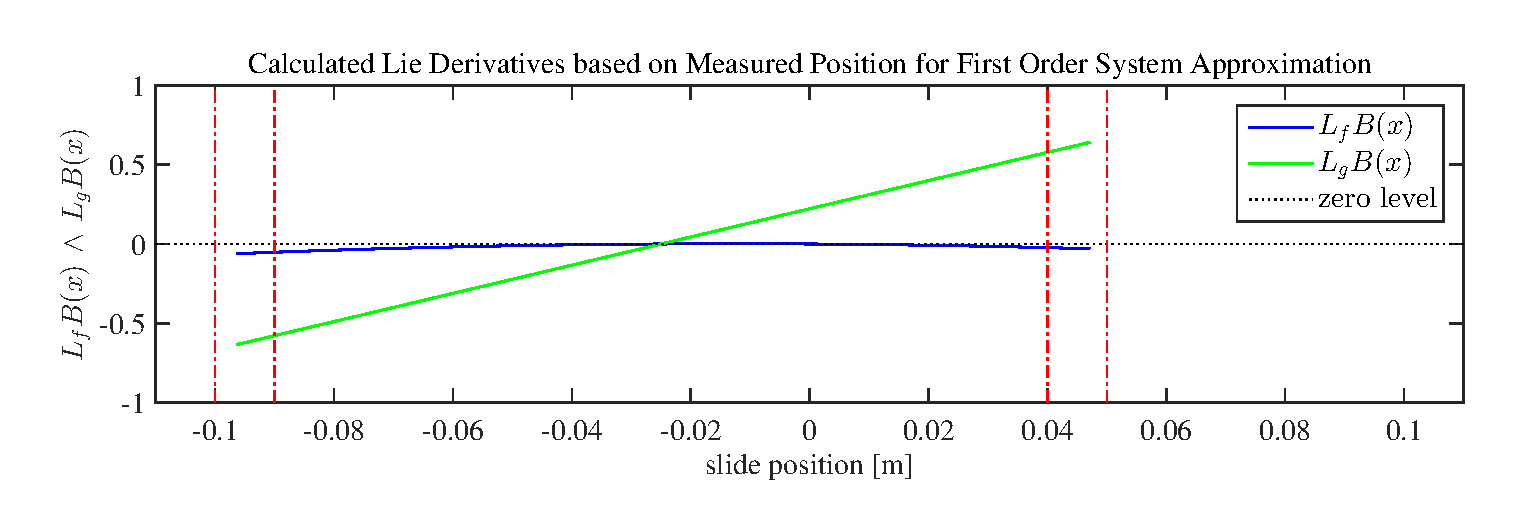
\includegraphics[scale=0.65]{meas_lie_1.eps}
	\caption{Calculated Lie derivatives based on measured position for the first order system approximation. }
    \label{fig:meas_lie_1}
\end{figure}
It is seen that the Lie derivatives from \autoref{fig:meas_lie_1} are very similar to the theoretical lie derivatives from \autoref{fig:lie1}.
%%%%%%%%%%%%
%%%%%%%%%%%%
%%%%%%%%%%%%
%%%%%%%%%%%%
\subsection{Implementation on the Da Vinci Robot based on 2D Model}\label{subsec-implement-2dmodel}
All plots and measurement in this subsection can be reconstructed by running the MATLAB script \texttt{plot\_data} found in \autoref{app:cd} in the folder \texttt{measurements/slide\_safety\_controller/2D\_2nd\_order}. Again, the execution time is validated first. A plot measuring the execution time for each iteration is shown in \autoref{fig:exe_1}.
\begin{figure}[H]
	\center
		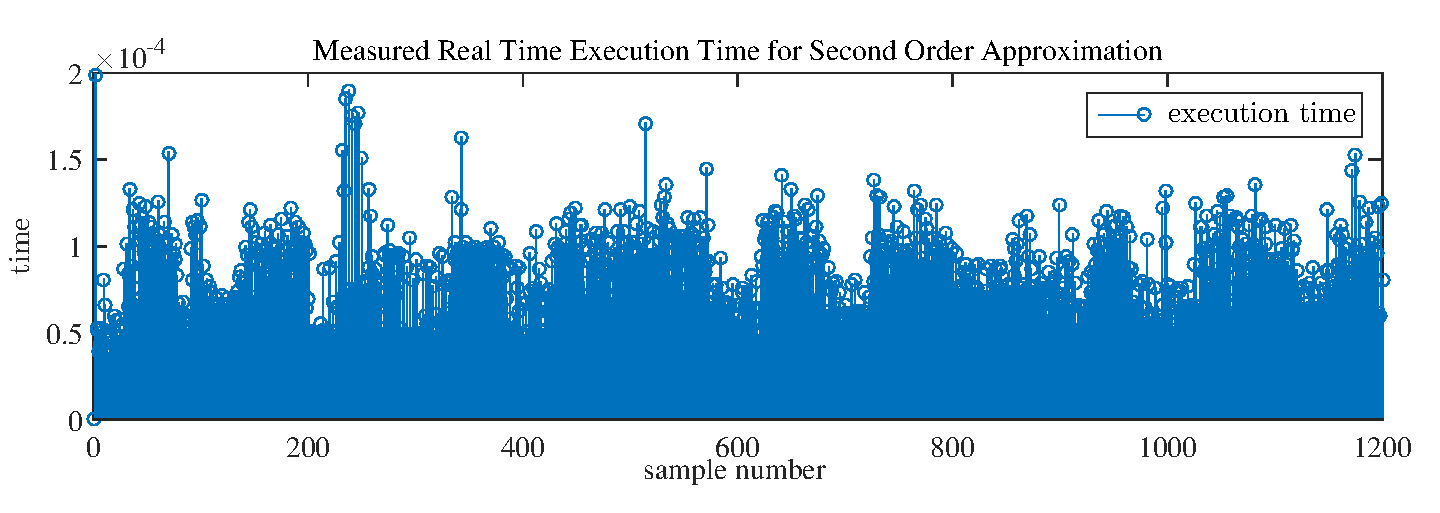
\includegraphics[scale=0.6]{execution_time_2_order.eps}
	\caption{Execution time for second order system approximation. It is seen that the controller never exceed at computation time of 200\,$\mu$s.}
	\label{fig:exe_2}
\end{figure}
It is from \autoref{fig:exe_2} seen that the real time part is completed within the allowed 10\,ms (100\,Hz). Note that the execution time is slightly higher than in \autoref{fig:exe_1} because the velocity is estimated with the observer.

The measured state trajectory is plotted in \autoref{fig:traj_meas_1}.
\begin{figure}[H]
	\center
		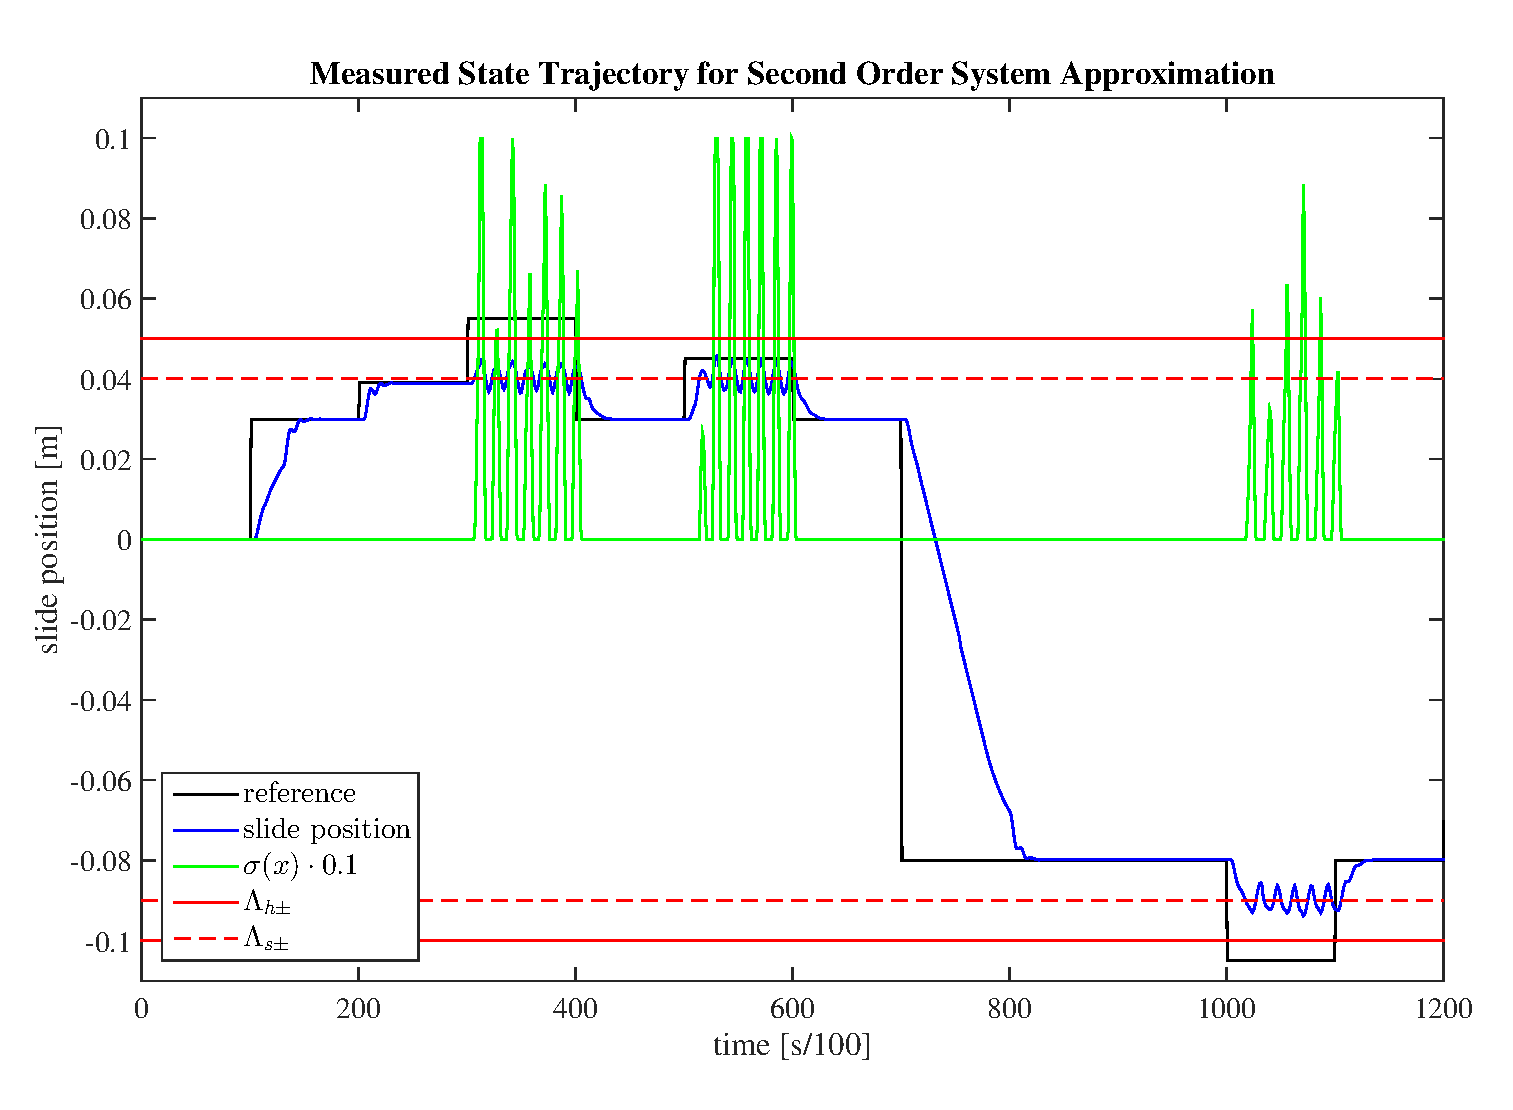
\includegraphics[scale=0.65]{meas_trajectory_2_order.eps}
	\caption{Measured position trajectory based on the second order approximation.}
    \label{fig:traj_meas_2}
\end{figure}
It is from \autoref{fig:traj_meas_2} seen how the overshoot is eliminated. This was indeed the main purpose of the development of a controller based on a second order approximation. Also, note how it is possible to give setpoints close to the the set $\mathcal{T}$ and still avoid oscillations caused by $\sigma(x)\neq 0$. This is a big advantage when a doctor needs to operate close to an unsafe regions. Finally, just as in \autoref{fig:traj_meas_1}, it is seen how $\sigma(x)$ forces the position below its setpoint when $x_\text{ref} \in \mathcal{X}_u$ but allows $x_1 > x_\text{ref}$ when $x \in \mathcal{T}$. This is indeed the effect of $\sigma(x)$.

The Lie derivatives are calculated based on the measured position and the estimated velocity. The result is seen in \autoref{fig:meas_lie_2}
\begin{figure}[H]
	\center
		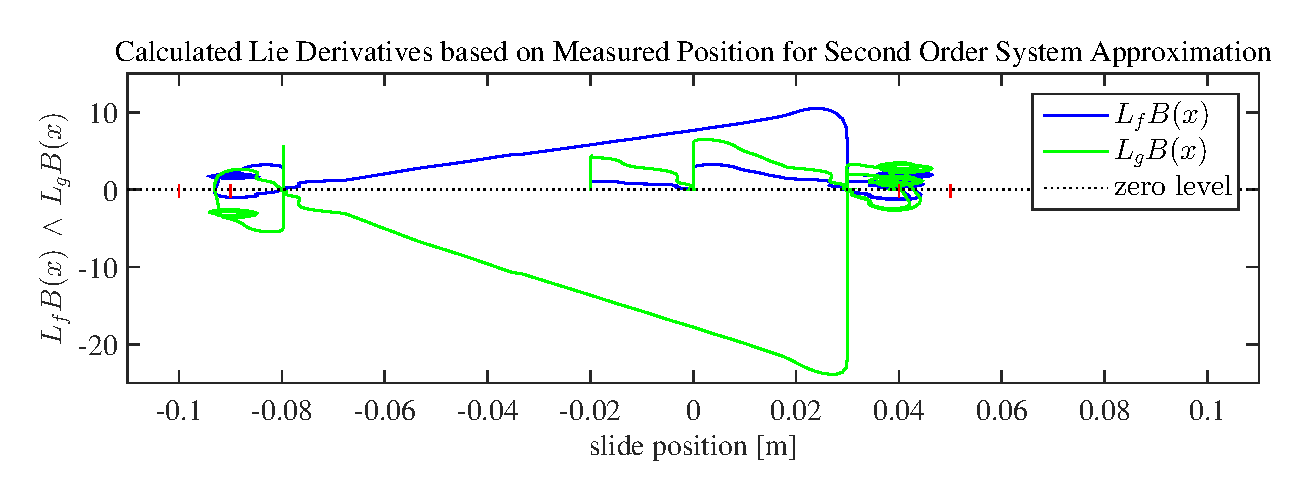
\includegraphics[scale=0.65]{meas_lie_2.eps}
	\caption{Calculated Lie derivatives based on measured position and estimated velocity for the second order system approximation. }
    \label{fig:meas_lie_2}
\end{figure}
It is seen that the Lie derivatives from \autoref{fig:meas_lie_2} are quite different that from \autoref{fig:lie2}. This is due to an imprecise estimation of the estimated velocity.
\subsection{Conclusion for Slide Safety Controller}\label{subsec:conclusion-slide-safety}
\chapter{Safety and Surgery on Beating Hearts} \label{chap:cbf_1d_dynamic}
\glsreset{cbf}
This chapter establishes the fundamentals for a system ensuring safety when a surgeon operates on a patient with a beating heart. In addition to the safety, it is the objective to establish a system with virtual fixture of the heart, i.e. such that the surgeon experiences the beating heart as static. As suggested by chief surgeon at Aalborg University Hospital, Johan Poulsen (see \autoref{sec:aau_doc}), a proper initial set-up emulating a beating heart could be a surface mounted on a cylinder moving periodically as a sinusoid. This scheme is outlined in \autoref{fig:dynamic_overview} illustrating how the virtual fixture of the heart should be obtained by dynamically positioning the end effector at a fixed distance from the surface of the heart.
\vspace{-2mm}
\begin{figure}[H]
%\hspace*{-10mm}
\subbottom[Terms]{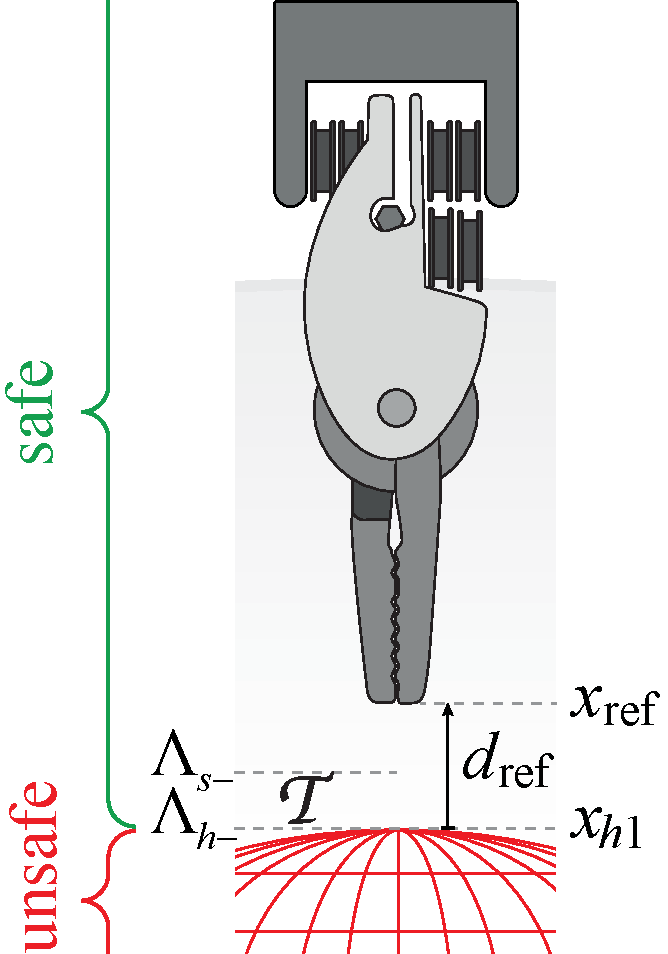
\includegraphics[height=4.2cm]{dynamic_boundary_limits.pdf}\label{fig:over_1}} \hspace{0.5cm}
\subbottom[Time sequence of a tool keeping a fixed distance  $d_\text{ref}$ to a moving surface]{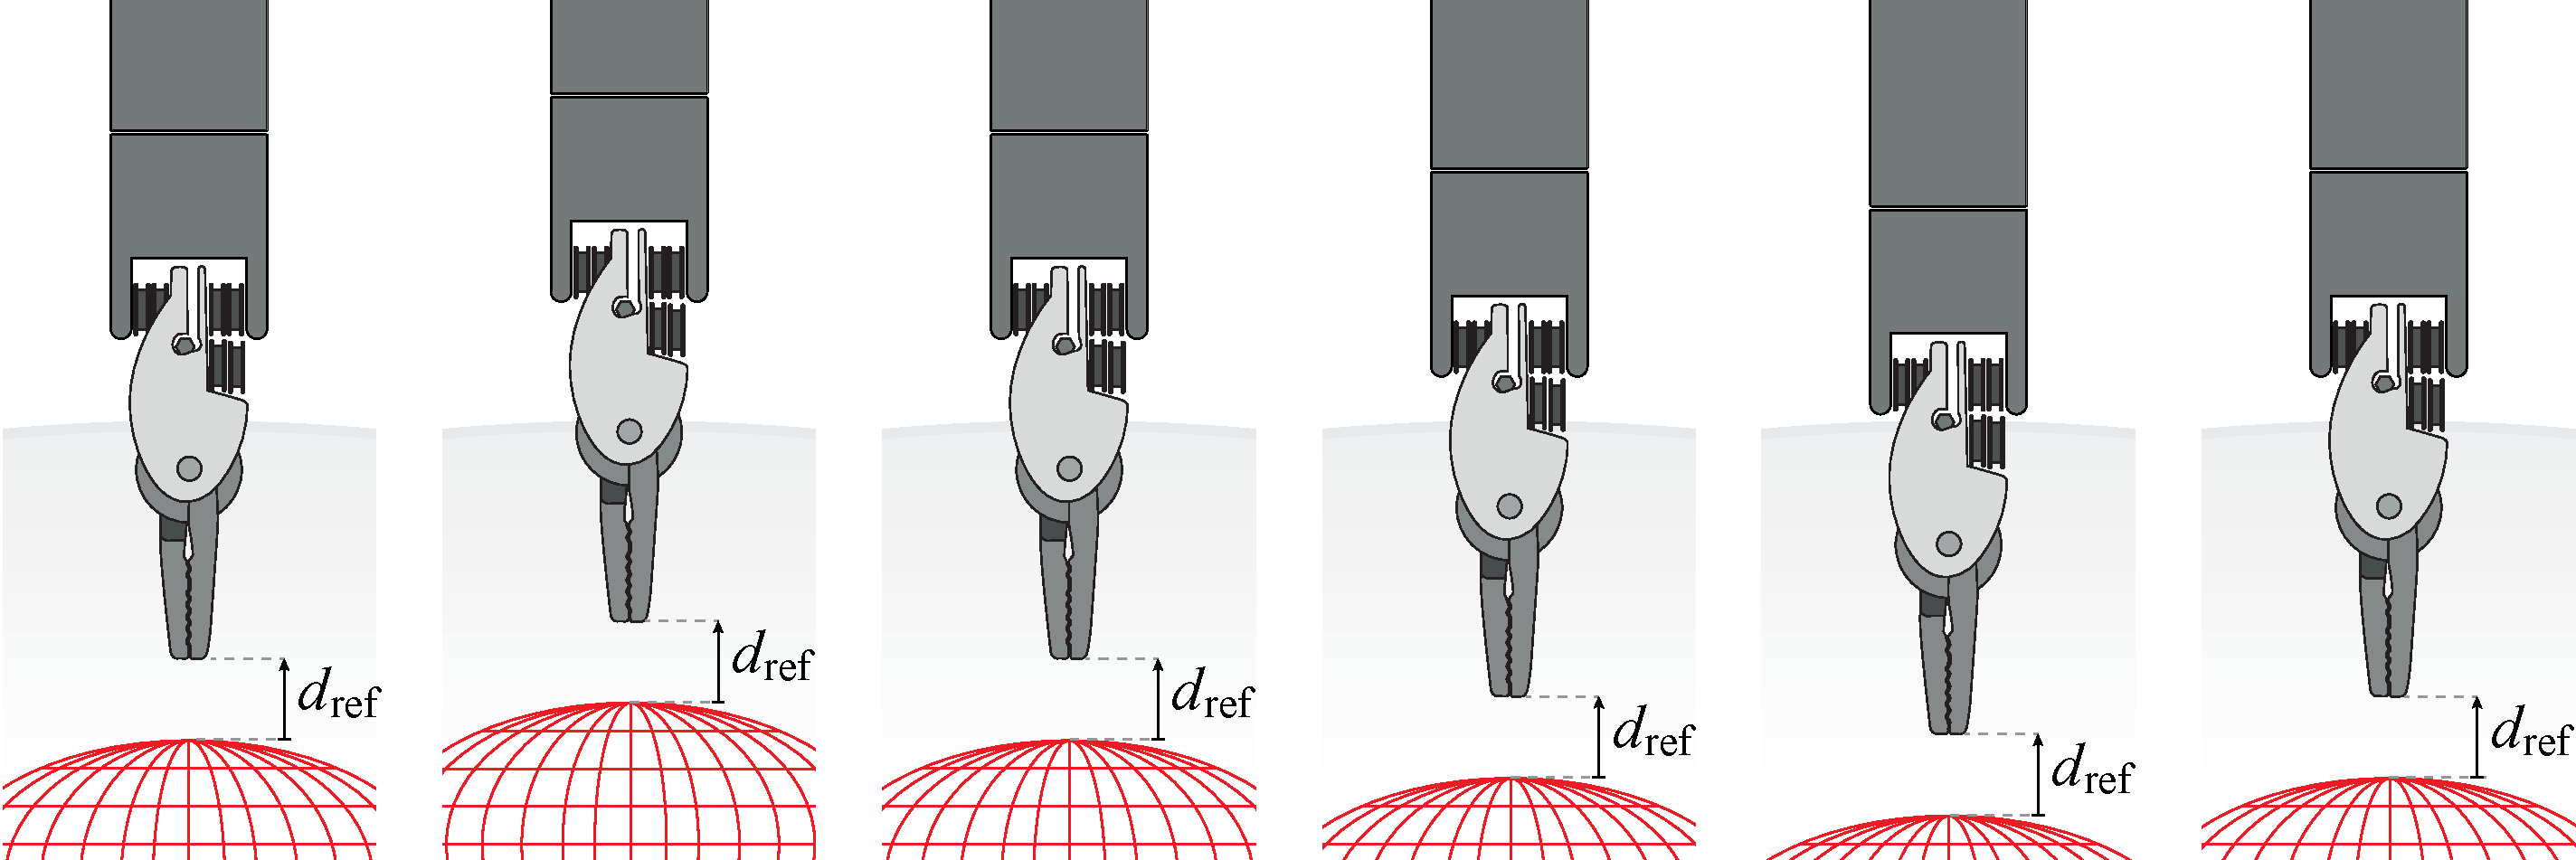
\includegraphics[height=4.2cm]{dynamic_boundary_sequence.pdf}\label{fig:over_2}}%
\caption{The objective is to attain a virtual fixture of the moving object by controlling the end effector distance to its surface, such that the surgeon experiences the object as static and can operate as if the object was in fact standing still. An overview of terms applied is found in \autoref{fig:over_1}.}
\label{fig:dynamic_overview}
\end{figure}
Thus a model of  heart movement is needed along with a model of the robot dynamics, such that a reference relative to the surface of the heart can be given. These models are presented in the following, after which a \gls{cbf} can be constructed and from this a controller is designed that ensures safety of the system.
%\begin{figure}[H]
%	\center
%		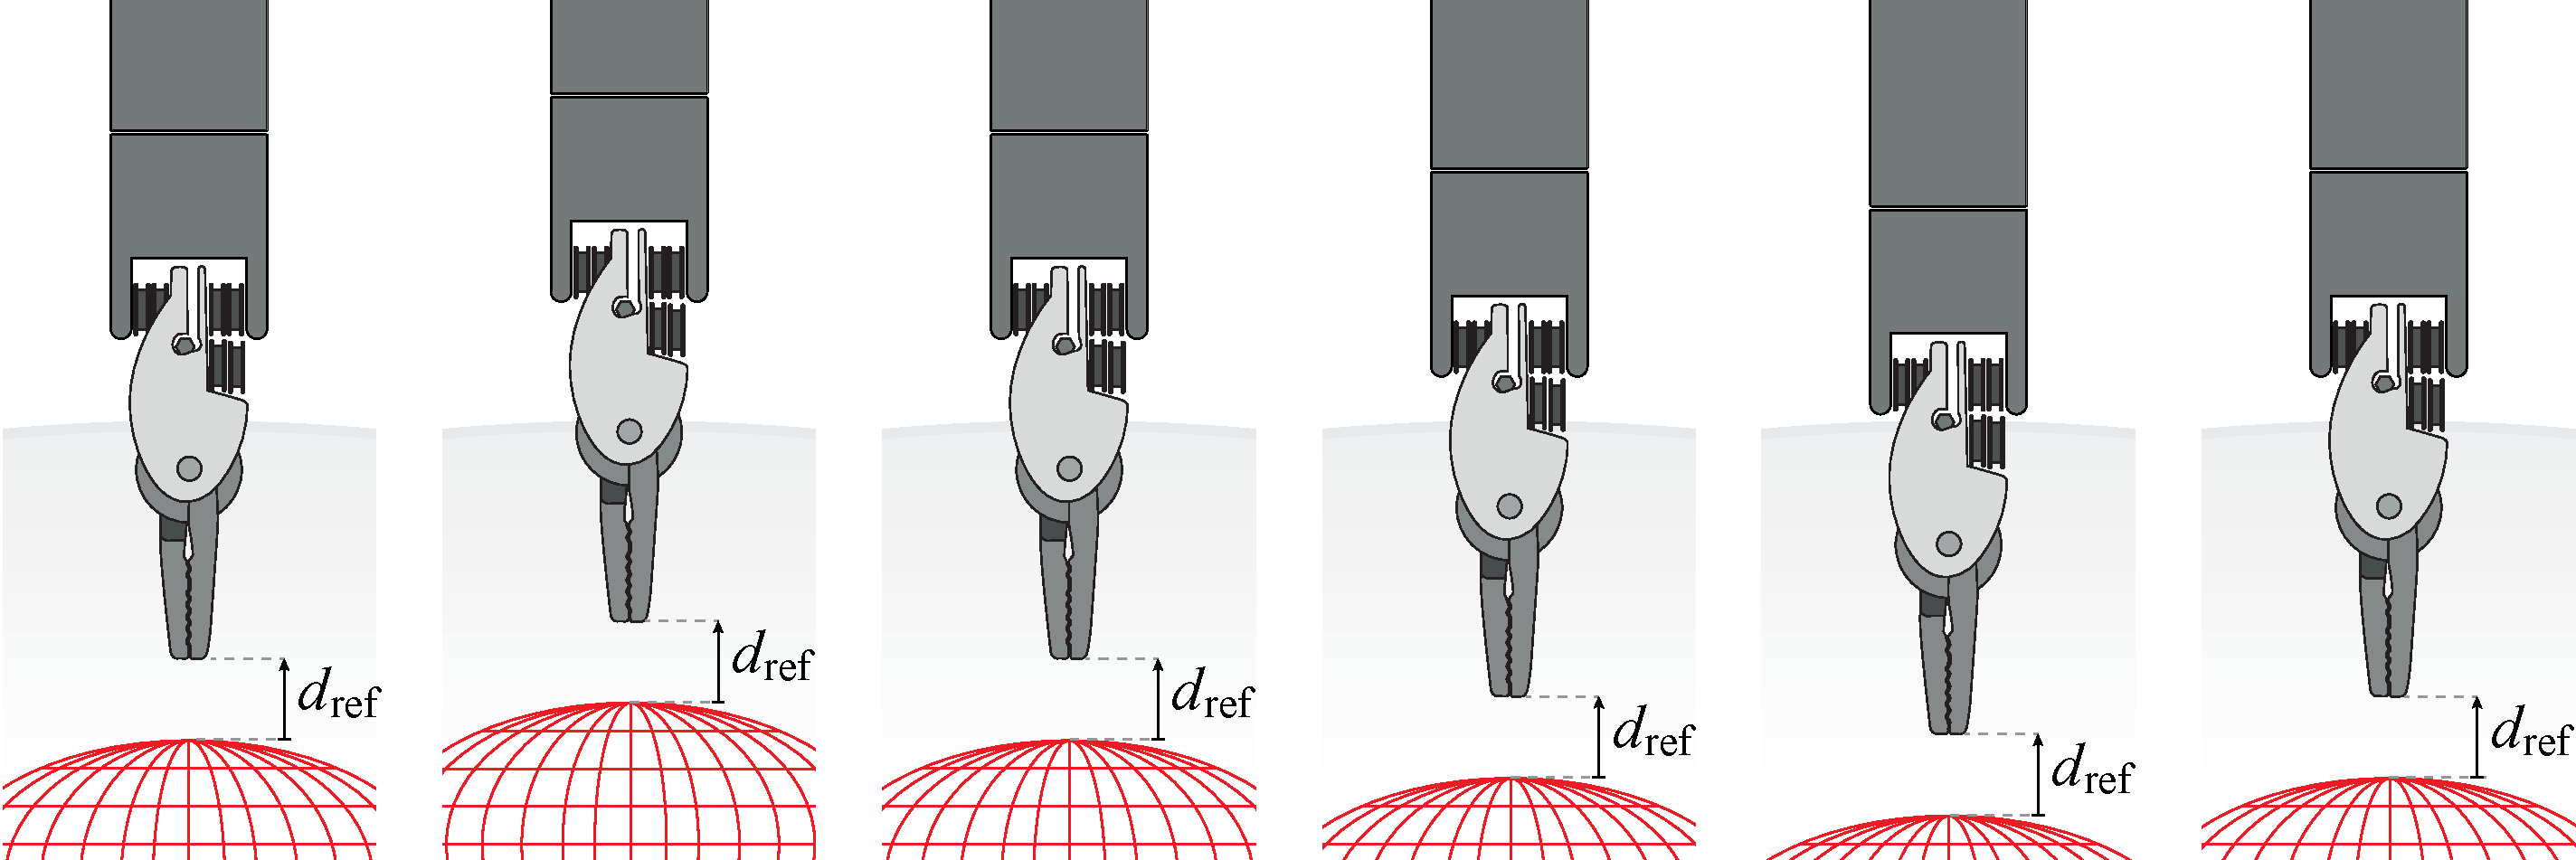
\includegraphics[width=1\textwidth]{dynamic_boundary_sequence.pdf}
%	\caption{lol.}
%	\label{fig:dynamic_overview}
%\end{figure}
%and..
%\begin{figure}[H]
%	\center
%		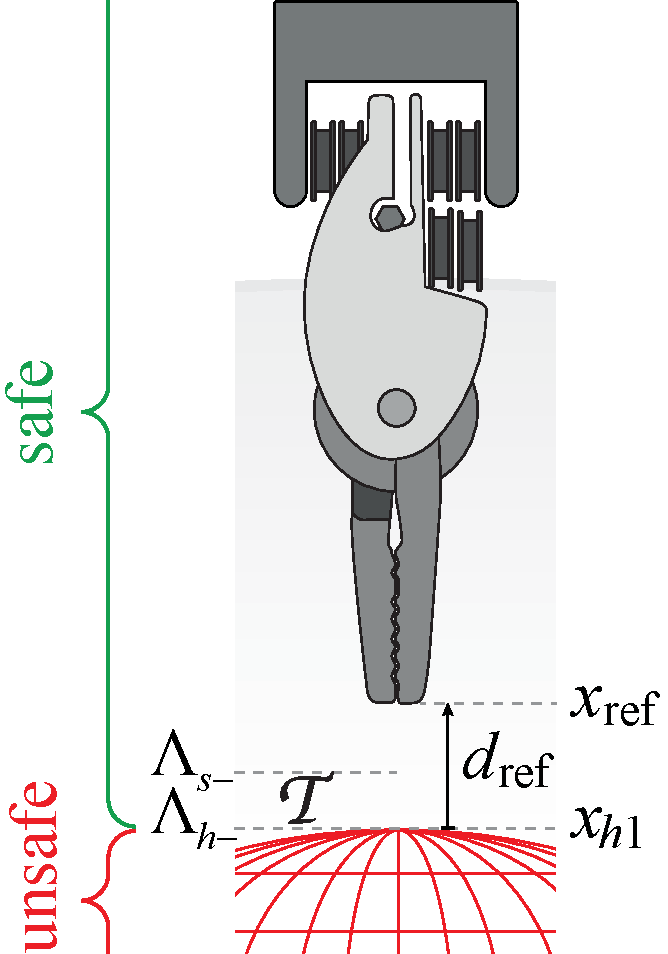
\includegraphics[width=0.2\textwidth]{dynamic_boundary_limits.pdf}
%	\caption{lol.}
%	\label{fig:dynamic_overview_2}
%\end{figure}
\section{Modelling the Dynamics of the System}
First a model of a beating heart is introduced. This is needed in order to be able to give a dynamic position reference such thath the end effector can be controlled to keep a fixed distance to the heart surface.
The the system model from \autoref{sec:model_slide} is recapitulated, and the dynamic reference is introduced through an augmented system.

\subsection{Modelling the Beating Heart as a Sinusoid}
\vspace{-2mm}
The simplified heart movement can be represented as a matrix with eigenvalues on the imaginary axis in the complex frequency domain:

\phantom{.}
\vspace{-15mm}
\begin{flalign}
\dot{\textbf{x}}_h =
\dot{\begin{bmatrix}
x_{h1}\\x_{h2}
\end{bmatrix}} =
\begin{bmatrix}
0 & \omega_h \\ -\omega_h & 0
\end{bmatrix}
\begin{bmatrix}
x_{h1}\\x_{h2}
\end{bmatrix} \kk \text{with} \kk \mathbf{x}_{h}(0) =\begin{bmatrix}
x_{h10} \\
x_{h20}
\end{bmatrix}
\label{eq:beating_heart_sine}
\end{flalign}
\begin{tabular}{rp{14cm}} 
where  &  \\
\gls{xh1}& is the position of a point on the surface of the heart \\
\gls{xh2}& is the velocity of the point \\
\gls{wh}& is the heartbeat frequency, $\omega_h = 2\pi/T_h$ rad/s with an average heartbeat period \gls{Th}$=1.1$\,s \citep{bib:heart_berkeley} \\
\gls{xh10} & is the initial value of $x_{h1}$ \\
\gls{xh20} & is the initial value of $x_{h2}$\\
\end{tabular}\\

Note that the magnitude of $\omega_h$ determines the frequency and that the initial conditions determine the amplitude of the heart oscillation, e.g. if $\mathbf{x}_h(0)=[0\mm 2]^T$ this indicates a sine with an amplitude of 2, while $\mathbf{x}_h(0)=[3\mm 0]^T$ corresponds to a cosine with an amplitude of 3. The heartbeat will with this system have a natural oscillation around zero. 

\subsection{Modelling the Robot Slide Movement}
\vspace{-1mm}
As in \autoref{chap:cbf_1d_static}, the slide movement of the robot is considered the  degree of freedom of the system, illustrated in \autoref{fig:slide}. To model the one dimensional robot movement along the slide axis, the same system model can be used as presented in \autoref{eq:1storder_1D_ss}, i.e.:
\vspace{-1mm}
\begin{flalign}
\dot{x}_1 = -\tau^{-1} x_1 + \tau^{-1} u
\label{eq:good_old}
\end{flalign}
\vspace{-1mm}
\begin{tabular}{rll}
where && \\
$x_1$ & is the position of the end effector & [m]\\
$\tau$ & is the time constant of the first order system, measured in \autoref{fig:stepresponseslide}, $\tau=110$\,ms & [s]\\
$u$ & is the input to the system & [m]\\
\end{tabular}\\

The one dimensional model is used to simplify the equations thus precluding complications at this stage. Additionally, the second order model merely proved few advantages in the form of elimination of the overshoot.

\vspace{-1mm}
\subsubsection*{Introducing a Dynamic Reference in the Model}

\vspace{-2mm}
In order to control the robot end effector to maintain a fixed distance to the surface of the heart, an additional state can be added the system. Thus, a new set of states is introduced representing the movement of the beating heart, the movement of the robot and the fixed distance \gls{dref} between the two.
%\begin{flalign*}
%\textbf{x} = \begin{bmatrix}
%x_1 \\ x_{h1} \\ x_{h2} \\ d_\text{ref}
%\end{bmatrix}
%\end{flalign*}
Combining \autoref{eq:beating_heart_sine} and \autoref{eq:good_old} with the relative distance yields the below stated linear state space system: 
\vspace{-3mm}
\begin{flalign}
\dot{\textbf{x}}(t) &= \dot{\begin{bmatrix}
	x_1\\x_{h1}\\x_{h2}\\ d_\text{ref}
	\end{bmatrix}} =
\underbrace{\underbrace{\begin{bmatrix}
		-1/\tau & 0 & 0 & 0\\0 & 0 & \omega_h & 0 \\ 0 & -\omega_h & 0 & 0 \\ 0& 0 & 0 & 0
		\end{bmatrix}}_{\textbf{A}}
	\begin{bmatrix}
	x_1\\x_{h1}\\x_{h2}\\ d_\text{ref}
	\end{bmatrix}}_{f(\mathbf{x})}+ 
\underbrace{\underbrace{\begin{bmatrix}
		1/\tau \\ 0 \\ 0 \\ 0
		\end{bmatrix}}_{\textbf{B}}}_{g(\mathbf{x})} \tilde{u}(x) \\
		\mathbf{y}(t) &= \underbrace{\begin{bmatrix}
		1 & 0 & 0 & 0
		\end{bmatrix}}_\textbf{C} \textbf{x}(t)
\end{flalign}	

The control law is introduced as a linear position controller on the form from \autoref{eq:utilde}, where the position reference follow the dynamic movement of the heart at a fixed distance $d_\text{ref}$ from its surface, i.e. $x_\text{ref} = x_{h1} + d_\text{ref}$ such that:
\vspace{-3mm}
\begin{flalign}
\tilde{u}(\mathbf{x}(t)) &= \bar{\mathbf{N}}x_\text{ref} - \mathbf{K}\,x_1 \nonumber\\
&= \bar{\mathbf{N}}\Big( x_{h1}(t)+ d_\text{ref} \Big)-\mathbf{K} x_1(t) \nonumber \\
%&= -\mathbf{K} x_1(t) + \bar{\mathbf{N}}x_{h1}(t) + \bar{\mathbf{N}} d_\text{ref}\nonumber \\
&= %\underbrace{
	\begin{bmatrix}
-\mathbf{K} & \bar{\mathbf{N}} & 0 & \bar{\mathbf{N}} 
\end{bmatrix}
%}_{\bar{\textbf{K}}} 
\textbf{x}(t) \nonumber\\
&= \bar{\textbf{K}} \textbf{x}(t)
\label{eq:utilde_dynamic}
\end{flalign}
\begin{tabular}{rp{14cm}}
where &\\
%$\tau$ & is the time constant of the first order system $\tau=0.11$\,s as given in \autoref{sec:model_slide}\\
$\mathbf{K}$ & is the linear system controller designed according to \autoref{eq:K_1}, $\mathbf{K} \in \mathbb{R}$ \\
$\bar{\textbf{N}}$ & is the system gain ensuring unity gain between position and reference, found according to \autoref{eq:barm_1}, $\bar{\mathbf{N}} \in \mathbb{R}$ \\
\gls{Kbar} & is the augmented feedback vector, $\bar{\textbf{K}} \in \mathbb{R}^{1 \times 4}$
\end{tabular}\\

%Such that:
%\begin{flalign}
%\tilde{u} = \bar{\textbf{K}} \textbf{x}
%\label{eq:utilde_dynamic}
%\end{flalign}
Note how the closed loop system can be rewritten in a more intuitive way, such that the system is reduced to three states taking $d_\text{ref}$ as input:
\vspace{-1mm}
\begin{flalign}
\dot{\begin{bmatrix}
	x_1\\x_{h1}\\x_{h2}\\d_\text{ref}
	\end{bmatrix}} &=
\underbrace{\underbrace{\begin{bmatrix}
		-1/\tau & 0 & 0 & 0\\0 & 0 & \omega_h & 0 \\ 0 & -\omega_h & 0 & 0 \\ 0& 0 & 0 & 0
		\end{bmatrix}}_{\textbf{A}}
	\begin{bmatrix}
	x_1\\x_{h1}\\x_{h2}\\d_\text{ref}
	\end{bmatrix}}_{f(\mathbf{x})}+ 
\underbrace{\underbrace{\begin{bmatrix}
		1/\tau \\ 0 \\ 0 \\ 0
		\end{bmatrix}}_{\textbf{B}}}_{g(\mathbf{x})}
\underbrace{\underbrace{\begin{bmatrix}
		-\mathbf{K} & \bar{\mathbf{N}} & 0 & \bar{\mathbf{N}}
		\end{bmatrix}}_{\bar{\textbf{K}}}
	\begin{bmatrix}
	x_1\\x_{h1}\\x_{h2}\\d_\text{ref}
	\end{bmatrix}}_{\tilde{u}(x)} \label{eq:cl_4states}\\
\dot{\begin{bmatrix}
	x_1\\x_{h1}\\x_{h2}
	\end{bmatrix}} &=
\underbrace{\begin{bmatrix}
	-(\mathbf{I}+\mathbf{K})/\tau & \bar{\mathbf{N}}/\tau & 0\\0 & 0 & \omega_h \\ 0 & -\omega_h & 0
	\end{bmatrix}}_{\textbf{A}_{cl}}
\begin{bmatrix}
x_1\\x_{h1}\\x_{h2}
\end{bmatrix}+ 
\underbrace{\begin{bmatrix}
	\bar{\mathbf{N}}/\tau \\ 0 \\ 0
	\end{bmatrix}}_{\textbf{B}_{cl}}
d_{ref}
\label{eq:cl_dynamic}
\end{flalign}
Note the eigenvalues of $\textbf{A}_{cl}$:
\vspace{-7mm}
\begin{flalign*}
\lambda_{\textbf{A}_{cl}} = \begin{cases}
-90 \\
5.71\,j \\
-5.71\,j
\end{cases}
\end{flalign*}
The eigenvalues reveal a stable (controllable) subsystem consisting of the robot end effector and an obviously marginally stable (uncontrollable) subsystem consisting of the beating heart.

This concludes the modelling of the augmented system. In the next section a \gls{cbf} will be constructed.
\vspace{-1mm}
\section{Construction of CBF}
\vspace{-3mm}
A barrier certificate for the system presented in \autoref{eq:cl_4states}, with a zero level set at the surface of the heart, comprises moving boundaries and hence should be a function of both robot and heart position. \Autoref{def:safety} implies that the \gls{cbf} should be constructed with unsafe region $\mathcal{X}_u$ below the surface of the heart, i.e. such that $B(\mathbf{x})$ is positive if $x_1<x_{h1}$ and negative otherwise, with $x_1$ being the position of the robot end effector and $x_{h1}$ being the position of the heart surface. The coherence is clear:
\vspace{-1mm}
\begin{equation}
B(\mathbf{x})>0 \mm \forall \,\,\,\mathbf{x}\in \mathcal{X}_u=\{(x_1,x_{h1}) \,\, | \,\, x_{h1}-x_1>0 \}
%x_{h1} - x_1 > 0 \kk  \Rightarrow \kk \mathbf{x} \in \mathcal{X}_u \kk\Leftrightarrow\kk B(\mathbf{x}) > 0 \nonumber
%\\
%-x_1 + x_{h1} &> 0 \kk  \\
%x_{h1} - x_1 &> 0 
\end{equation}

\vspace{-2mm}
Thus a \gls{cbf} can be constructed as:
\vspace{-4mm}
\begin{flalign}
B(\mathbf{x})= \tilde{c}(x_{h1}-x_1)\label{eq:barrier_dynamic}
\end{flalign}

\vspace{-1mm}
with a positive constant $\tilde{c}>0$, which is chosen to be $\tilde{c}=1$. %Setting $\tilde{c} = 1$ yields a 1:1 mapping which indeed will be the case here. 
Thus according to \autoref{def:cbf} this is a valid CBF if $L_gB(\mathbf{x}) \neq 0$ and $\{\mathbf{x} \in \mathcal{X} \,\, | \,\, B(\mathbf{x}) \leq 0 \} \neq \emptyset$. The latter  is trivial as the safe states are present whenever $x_1>x_{h1}$. Thus  $L_gB(\mathbf{x})$ is analysed:
\begin{flalign}
L_gB(\mathbf{x}) = \frac{d B(\mathbf{x})}{ d \textbf{x}}g(\mathbf{x}) \Biggm|_{g(\mathbf{x}) = \textbf{B}}  
&= \begin{bmatrix}
\dfrac{\partial B(\mathbf{x})}{\partial x_1} & \dfrac{\partial B(\mathbf{x})}{\partial x_{h1}} & \dfrac{\partial B(\mathbf{x})}{\partial x_{h2}} & \dfrac{\partial B(\mathbf{x})}{\partial d_\text{ref}}
\end{bmatrix} \textbf{B} \nonumber \\
&= \begin{bmatrix}
-\tilde{c} & \tilde{c} & 0 & 0
\end{bmatrix}
\begin{bmatrix}
1/\tau\\
0 \\ 0 \\ 0
\end{bmatrix} \Bigm|_{\tilde{c}=1}  =
\frac{-1}{\tau} \neq 0 \quad \forall \, \mathbf{x} \in \mathcal{X}
\label{eq:lgb_dynamic}
\end{flalign}
It is seen that $L_gB(\mathbf{x}) \neq 0$ for all $\mathbf{x} \in \mathcal{X}$. The \gls{cbf} is therefore valid on $\mathcal{X}$.

\section{Control Design}
As introduced in \autoref{eq:u_utilde_k0}, the safe set $\mathcal{X}_0$ can be divided into two sections: the transitions space $\mathcal{T}$ close to the unsafe set and the remaining part $\mathcal{Y}=\mathcal{X}_0\setminus\mathcal{T}$. These sections are indicated in \autoref{fig:over_1}.
The control law is, just as in \autoref{chap:cbf_1d_static}, split in two parts. A linear controller where no safety precautions are taken is used in $\mathcal{Y}$ and a controller ensuring safety is used in $\mathcal{T} \bigcup \mathcal{X}_u$. The controller ensuring safety is defined in \autoref{eq:control_law_safety}.

The transition between the two controllers on $\mathcal{T}$ is determined by $\sigma(\mathbf{x})$ which is defined in \autoref{eq:smoothness}. Thus a scalar $\epsilon$ is required,  determining when the effect of the safety controller $k_0(\mathbf{x})$ is brought into effect, while the weighting of $k_0(\mathbf{x})$ is determined by $\sigma(\mathbf{x})$. To give the safety controller some margin to force the robot end effector away from $\mathcal{X}_u$, it is reasonable to let $k_0(\mathbf{x})$ take effect when the end effector comes within a distance from the unsafe set of 1\,cm, thus:
\vspace{-3mm}
\begin{flalign}
\epsilon = 0.01\label{eq:epsilon_dynamic}
\end{flalign}

%\vspace{-3mm}
%Thus $\sigma(x)$ can be stated as:
%\begin{flalign}
%\sigma(x) = 
%\begin{cases}
%0 & \text{if} \mm B(x_1,x_{h1}) \leq -\epsilon \\
% -2  \left( \dfrac{B(x_1,x_{h1}}{\epsilon} \right)^3 - 3\left( \dfrac{B(x_1,x_{h1})}{\epsilon} \right)^2 +1  \kk &\text{if} \mm B(x_1,x_{h1}) \in (-\epsilon,0) \\
%1  &\text{if} \mm B(x_1,x_{h1}) \geq 0
%\end{cases}
%\label{eq:sig_dynamic}
%\end{flalign} 
The safety controller, as defined in \autoref{eq:control_law_safety}, requires  the Lie derivatives of the CBF, where $L_gB(\mathbf{x})$ is found in \autoref{eq:lgb_dynamic}, and $L_fB(\mathbf{x})$ is found as:
\begin{flalign}
L_fB(\mathbf{x}) &= \frac{dB(\mathbf{x})}{d\textbf{x}}f(\textbf{x})\Bigm|_{f(\textbf{x})=\textbf{A}\textbf{x}} \nonumber \\
&= \begin{bmatrix}
\dfrac{\partial  B(\mathbf{x})}{\partial x_1 } & \dfrac{\partial  B(\mathbf{x})}{\partial x_{1h} } & \dfrac{\partial  B(\mathbf{x})}{\partial x_{2h} } & \dfrac{\partial  B(\mathbf{x})}{\partial d_\text{ref} }
\end{bmatrix}  \begin{bmatrix}
1/\tau & 0 & 0 & 0 \\
0 & 0 & \omega_h & 0 \\
0 & -\omega_h & 0 & 0 \\
0 & 0 & 0 & 0 
\end{bmatrix} \begin{bmatrix}
x_1 \\ x_{x1} \\ x_{x2} \\ d_\text{ref}
\end{bmatrix} \nonumber \\
&=
\begin{bmatrix}
-\tilde{c} & \tilde{c} & 0 & 0
\end{bmatrix}
\begin{bmatrix}
-x_1/\tau\\
\omega_h x_{h2} \\
-\omega_h x_{h1} \\
0
\end{bmatrix} =
\tilde{c}\left(\omega_h x_{h2} + \frac{ x_1}{\tau}\right) \Bigm|_{\tilde{c}=1} = \omega_hx_{h2} + \dfrac{x_1}{\tau}
\label{eq:Lf_dynamic}
\end{flalign}

\begin{recap}[Control Law for Dynamic System with Relative Reference]
Using \autoref{eq:control_law}, the control law can be summarized as:
\begin{flalign*}
u(\mathbf{x}) = \sigma(\mathbf{x})k_0(\mathbf{x}) + (1-\sigma(\mathbf{x}))\tilde{u}(\mathbf{x})
\end{flalign*}
\begin{tabular}{rp{12.5cm}} 
where  &  \\
$\sigma(\mathbf{x})$ & is calculated from \autoref{eq:smoothness} with $B(\mathbf{x})$ found in \autoref{eq:barrier_dynamic} and $\epsilon$ found in \autoref{eq:epsilon_dynamic}\\
$k_0(\mathbf{x})$ & is calculated from \autoref{eq:control_law_safety} with the Lie derivatives from \ref{eq:lgb_dynamic} and \ref{eq:Lf_dynamic} \\
$\tilde{u}(\mathbf{x})$ & is calculated from \autoref{eq:utilde_dynamic}
\end{tabular}\\
\end{recap}
This completes the control design.

\section{MATLAB Implementation and Results}
The results presented in this section are implemented with the following characteristics:
\vspace{-2mm}
\begin{itemize}
	\itemsep-0.7mm
\item Extrapolation by means of forward Euler.
\item A sampling rate $f_s=2\,$kHz. The current realistic sampling rate at $f_s=100\,$Hz is not plotted as the forward Euler method proves itself unstable for this system at a 100\,Hz sampling rate.
\item Simulation time is 5\,s.
\item The distance $d_\text{ref}$ is initially set to 3\,cm which is safe. At 2\,s the reference distance $d_\text{ref}$ is altered to -1\,cm emulating a surgeon who accidentally forced the robot to penetrate the heart. The expected outcome of this is obviously that the safety controller prevents this by ensuring a distance between end effector and the beating heart.
\item Initial conditions are set such that the robot end effector is positioned at a distance to the heart greater than the desired distance. The expected outcome is that the system will attempt to track the distance $x_\text{ref}-x_{h1}=d_\text{ref}$.
\end{itemize}
The MATLAB implementation itself can be found in \autoref{app:slide_implement_1} and in \autoref{app:cd} under the path \texttt{matlab\_scripts/beating\_heart/beating\_heart\_controller.m}. The state trajectory is plotted in \autoref{fig:matlab_dynamics}.

\vspace{-2mm}
\begin{figure}[H]
	\center
		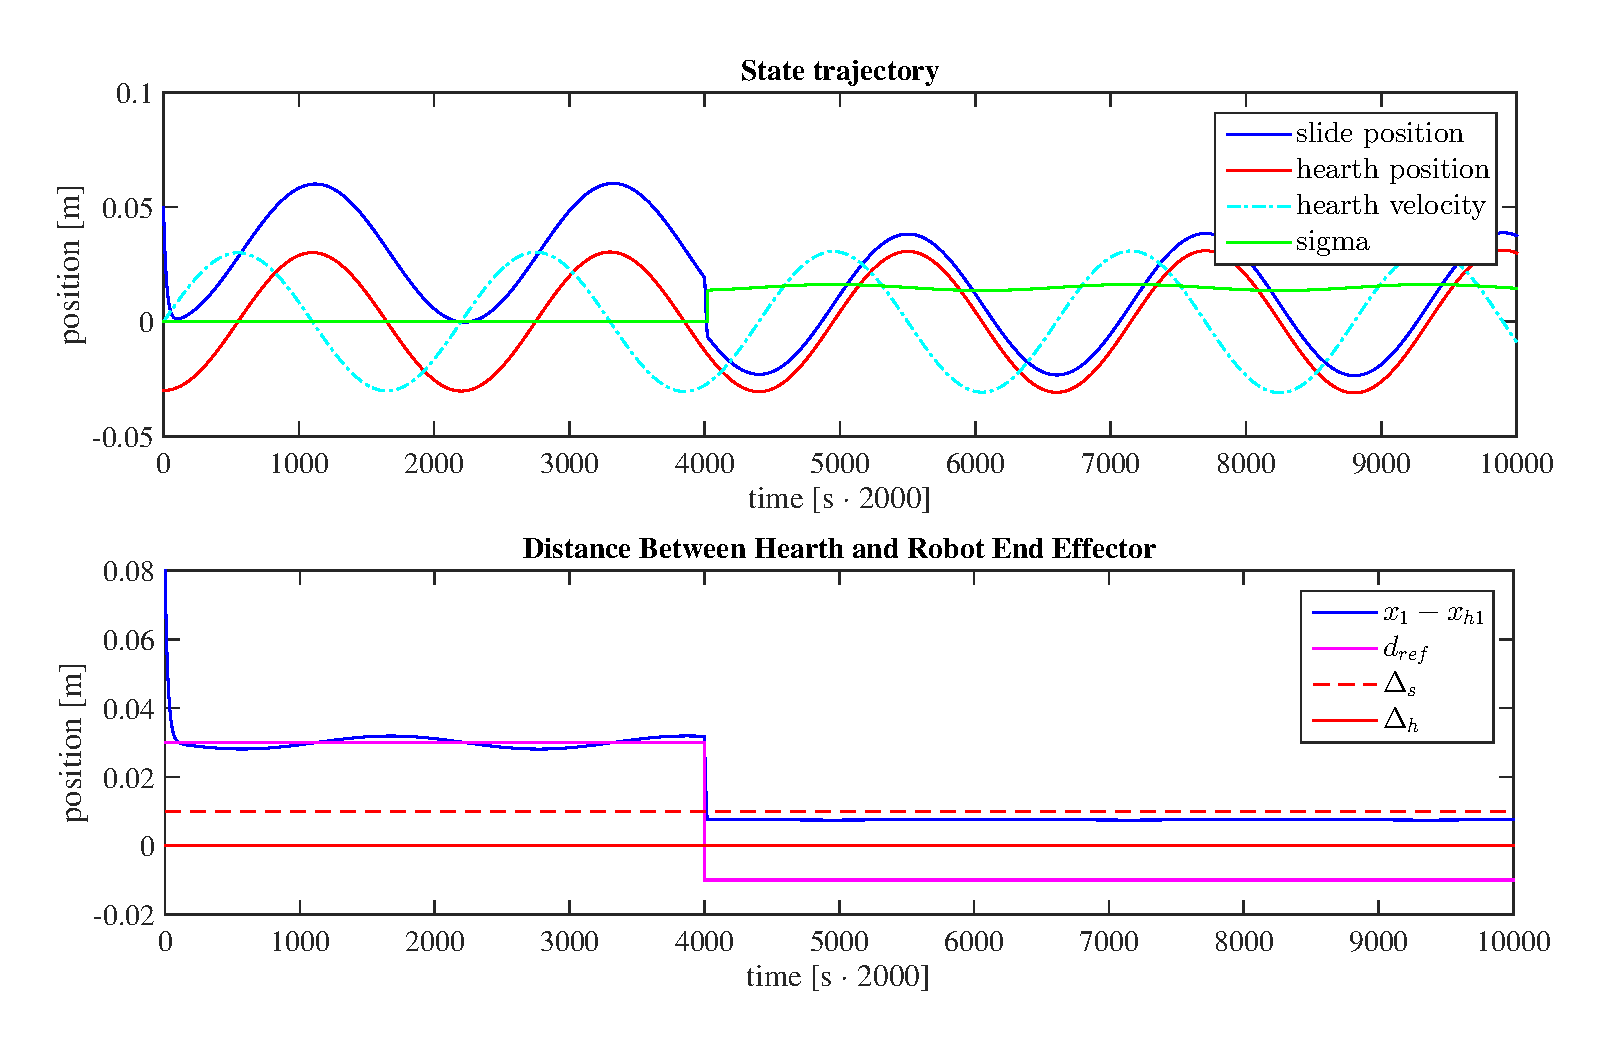
\includegraphics[width=1\textwidth]{state_trajectory_dynamic_matlab.eps}
	\caption{Dynamic system with heart position defined as the zero level set of the CBF. References are given as relative distances to the moving surface. When a reference outside the safe region is given, the safety controller prevents the tool from entering the unsafe region.}
    \label{fig:matlab_dynamics}
\end{figure}
It is from \autoref{fig:matlab_dynamics} seen that the robot end effector settles at a distance at $d_\text{ref}=3\,$cm until the simulation reaches 2\,s ($k=4000$). It is, however, seen that $d_\text{ref}$ is not constant which is due to the lack of integral action in the system. This could obviously be resolved by including integral action in the controller.  At 2\,s $d_\text{ref}$ changes to -1\,cm which causes the safety controller to react. The state $x_1$ settles at a safe distance from the beating heart which is left untouched, and the simulated controller is thereby verified to work as intended.

\vspace{-0.2cm}
\section{Implementation on the da Vinci Robot}
\vspace{-0.2cm}

For the implementation of the beating heart controller, the setup depicted in \autoref{fig:beatingheart_setup} is used. A tissue phantom representing the heart is mounted on top of a cylinder controlled by a motor to move in a sinusoid. In the motor controller interface the amplitude, frequency and offset of the sinusoid can be set.%
\begin{figure}[h]
	\centering
	\subbottom{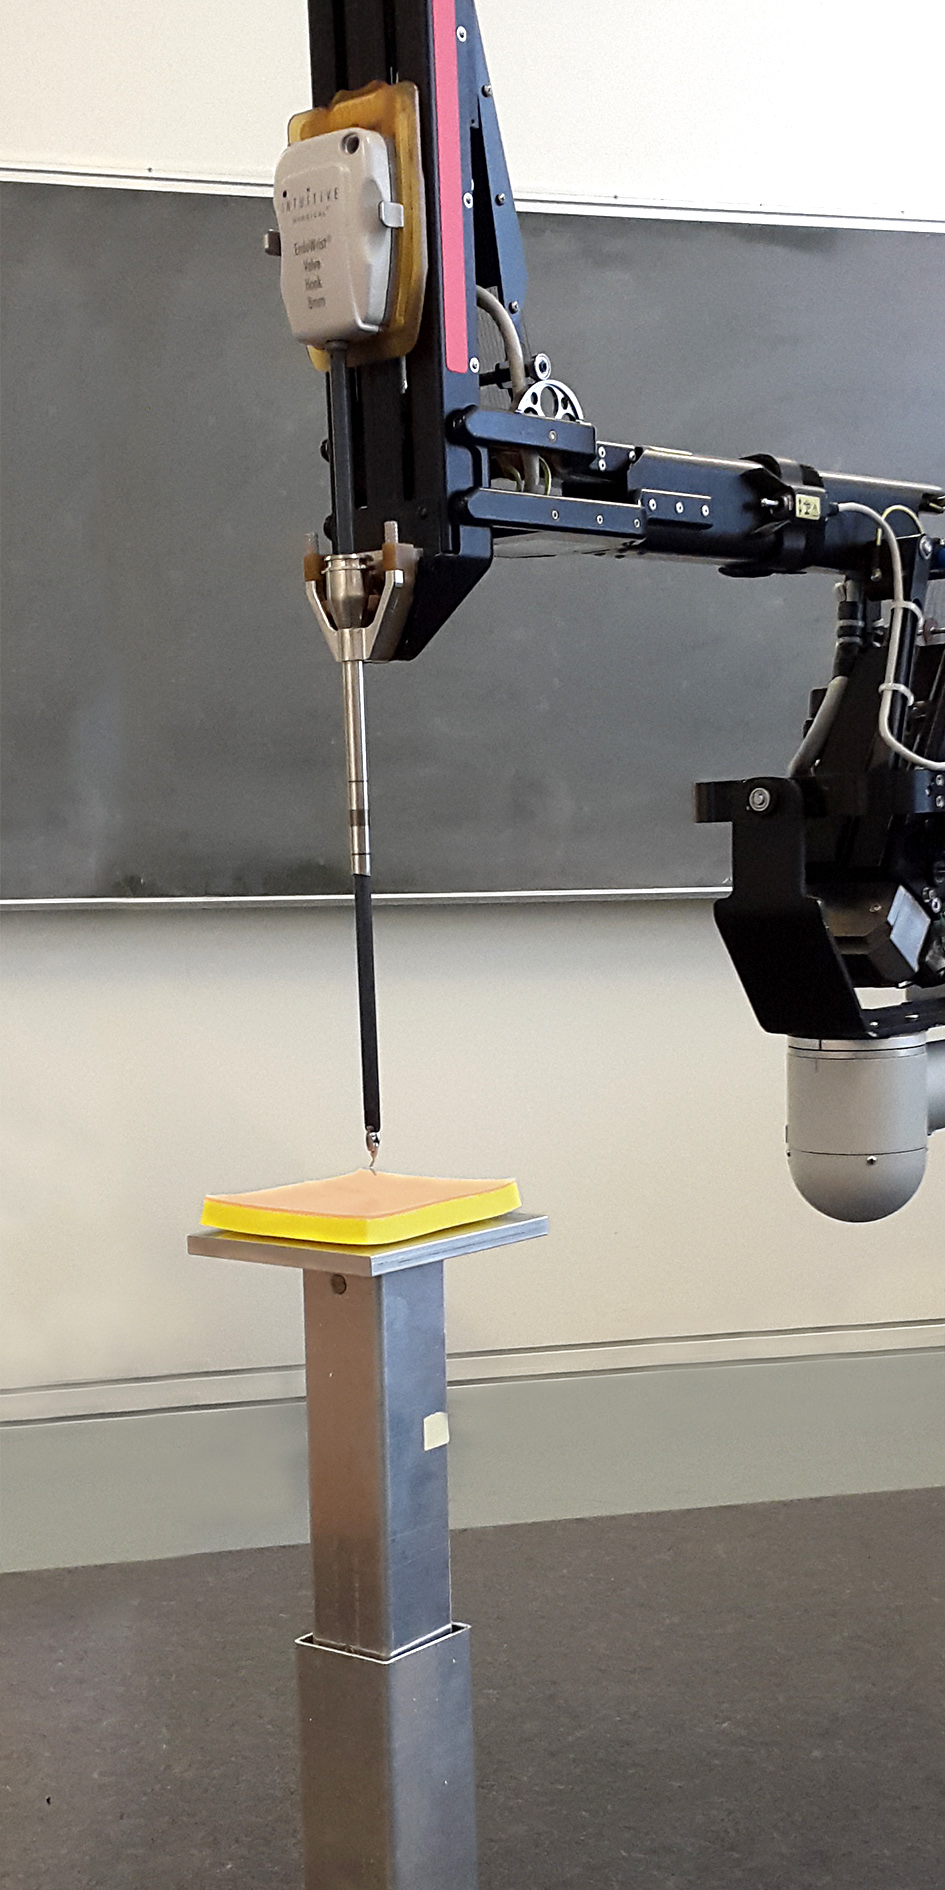
\includegraphics[width=0.23\textwidth]{20150531_171620.jpg}}%
	\hspace{2mm}
	\subbottom{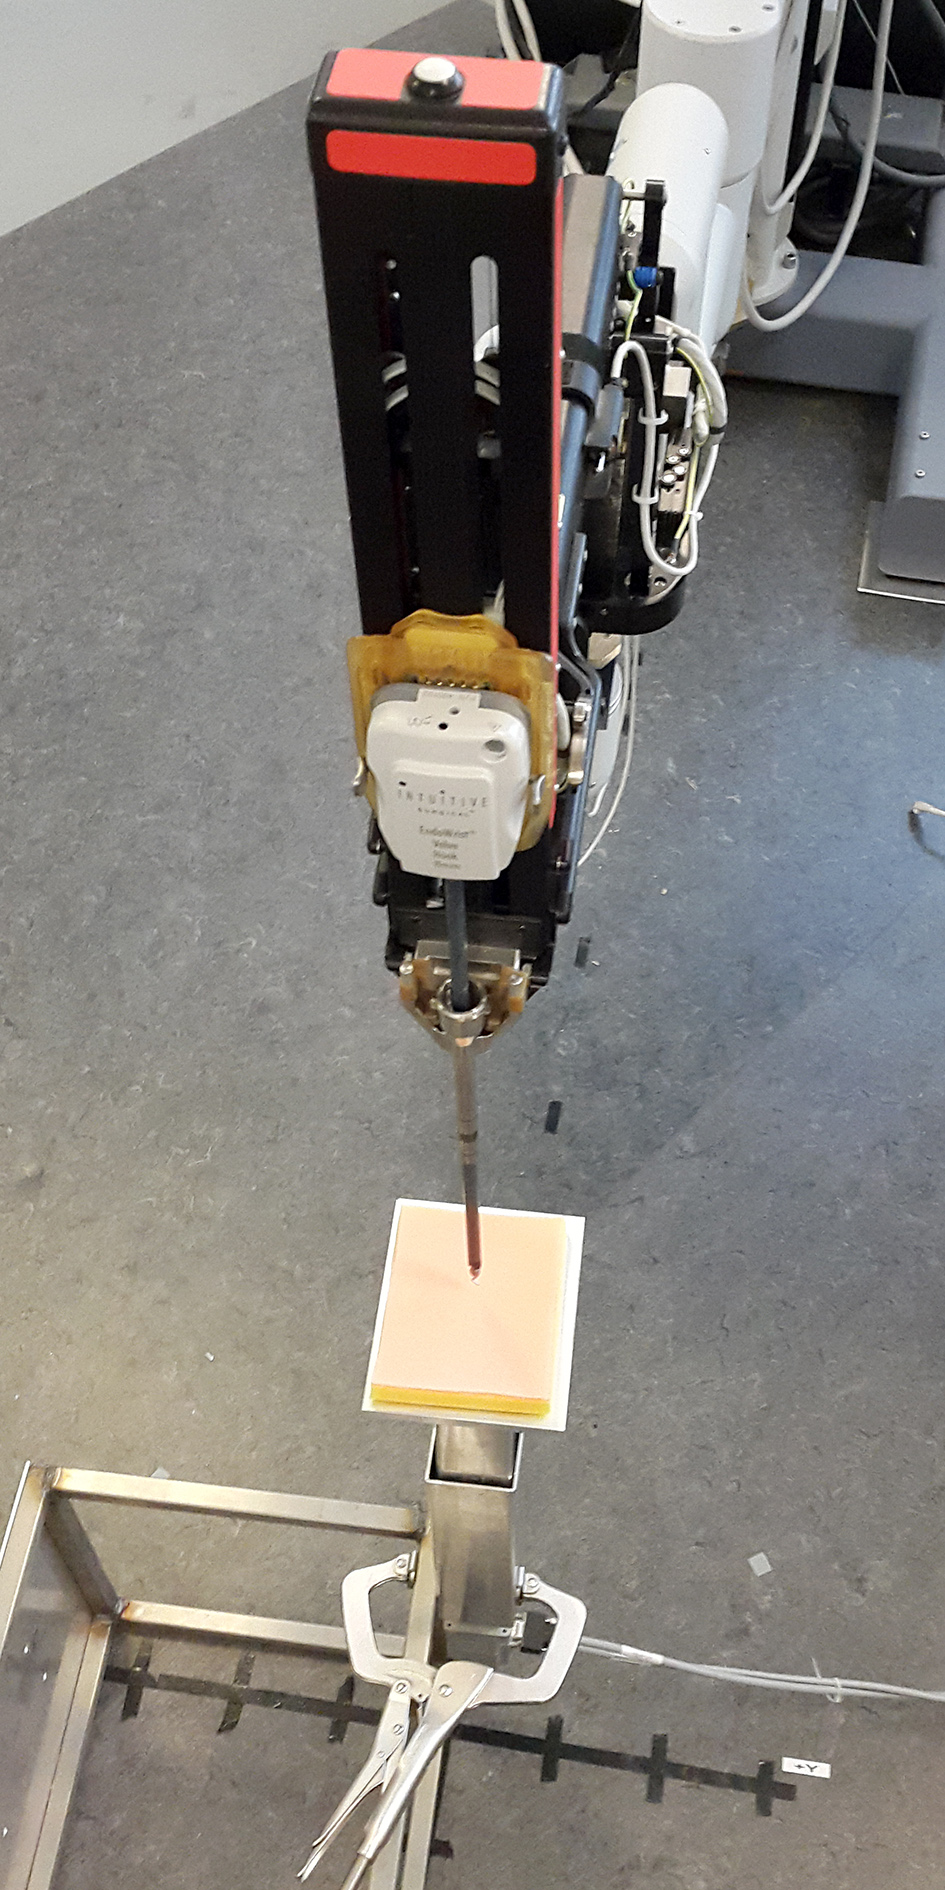
\includegraphics[width=0.23\textwidth]{20150531_171904.jpg}}%
	\hspace{2mm}
	\subbottom{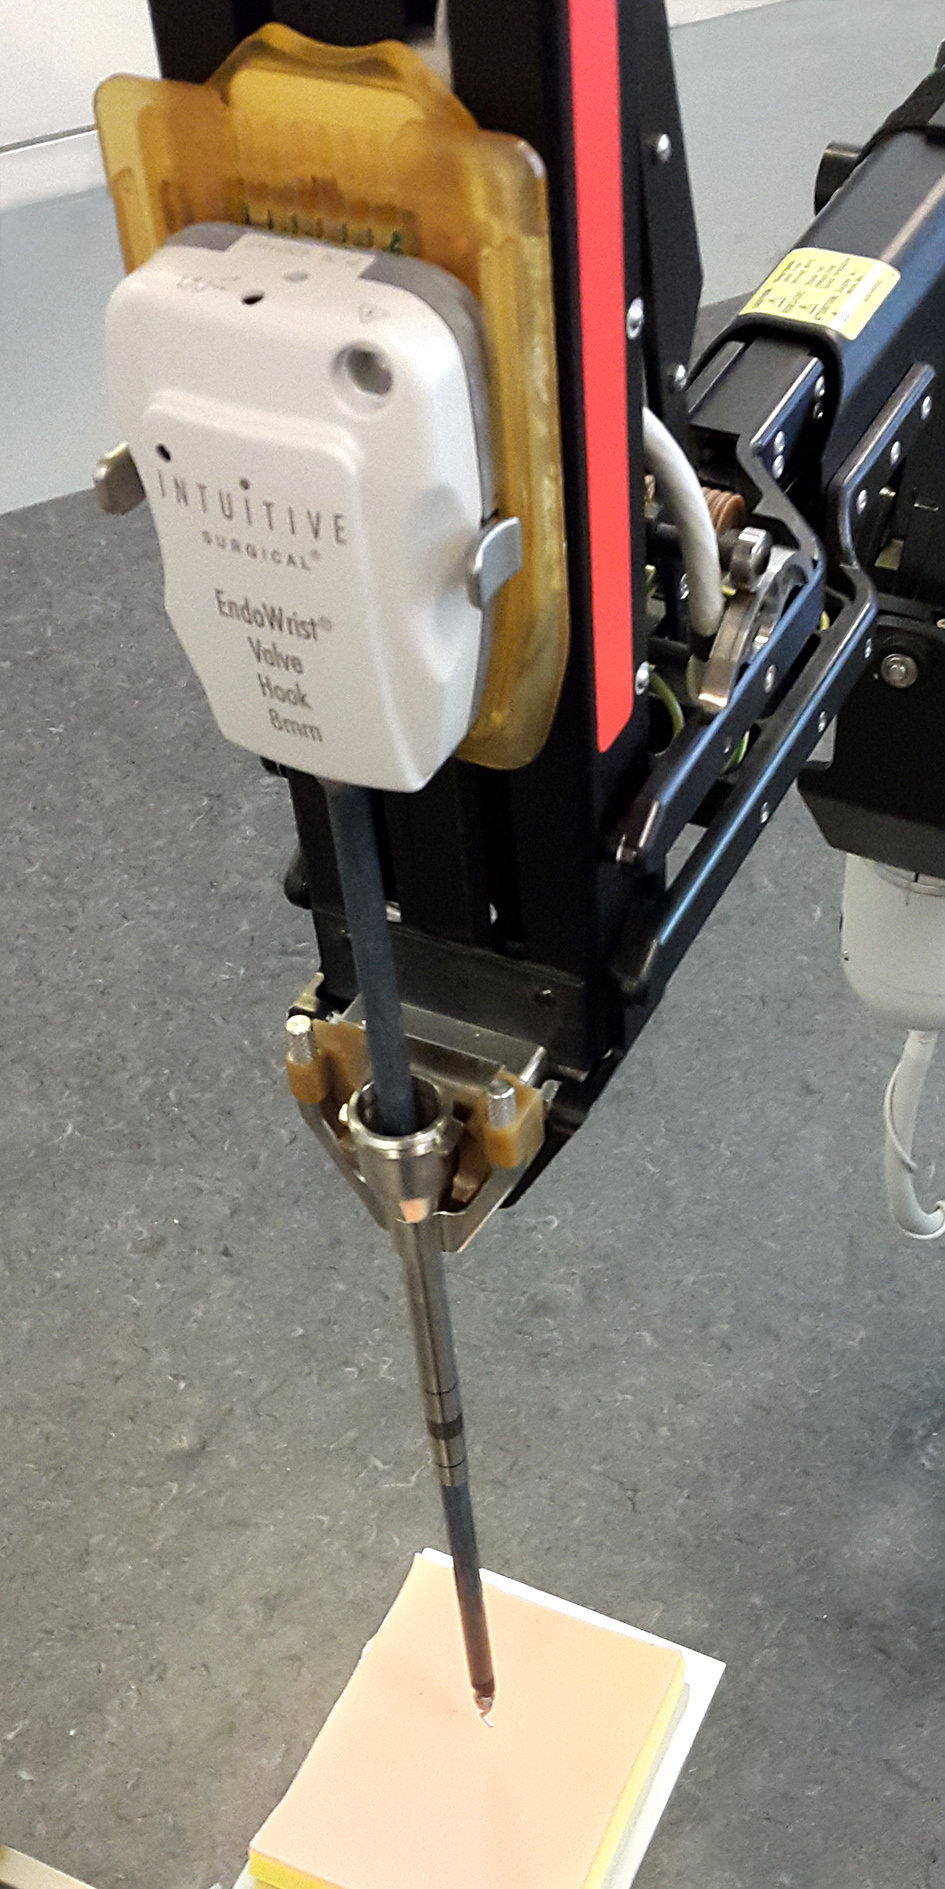
\includegraphics[width=0.23\textwidth]{20150531_171531.jpg}}%
	\hspace{2mm}
	\subbottom{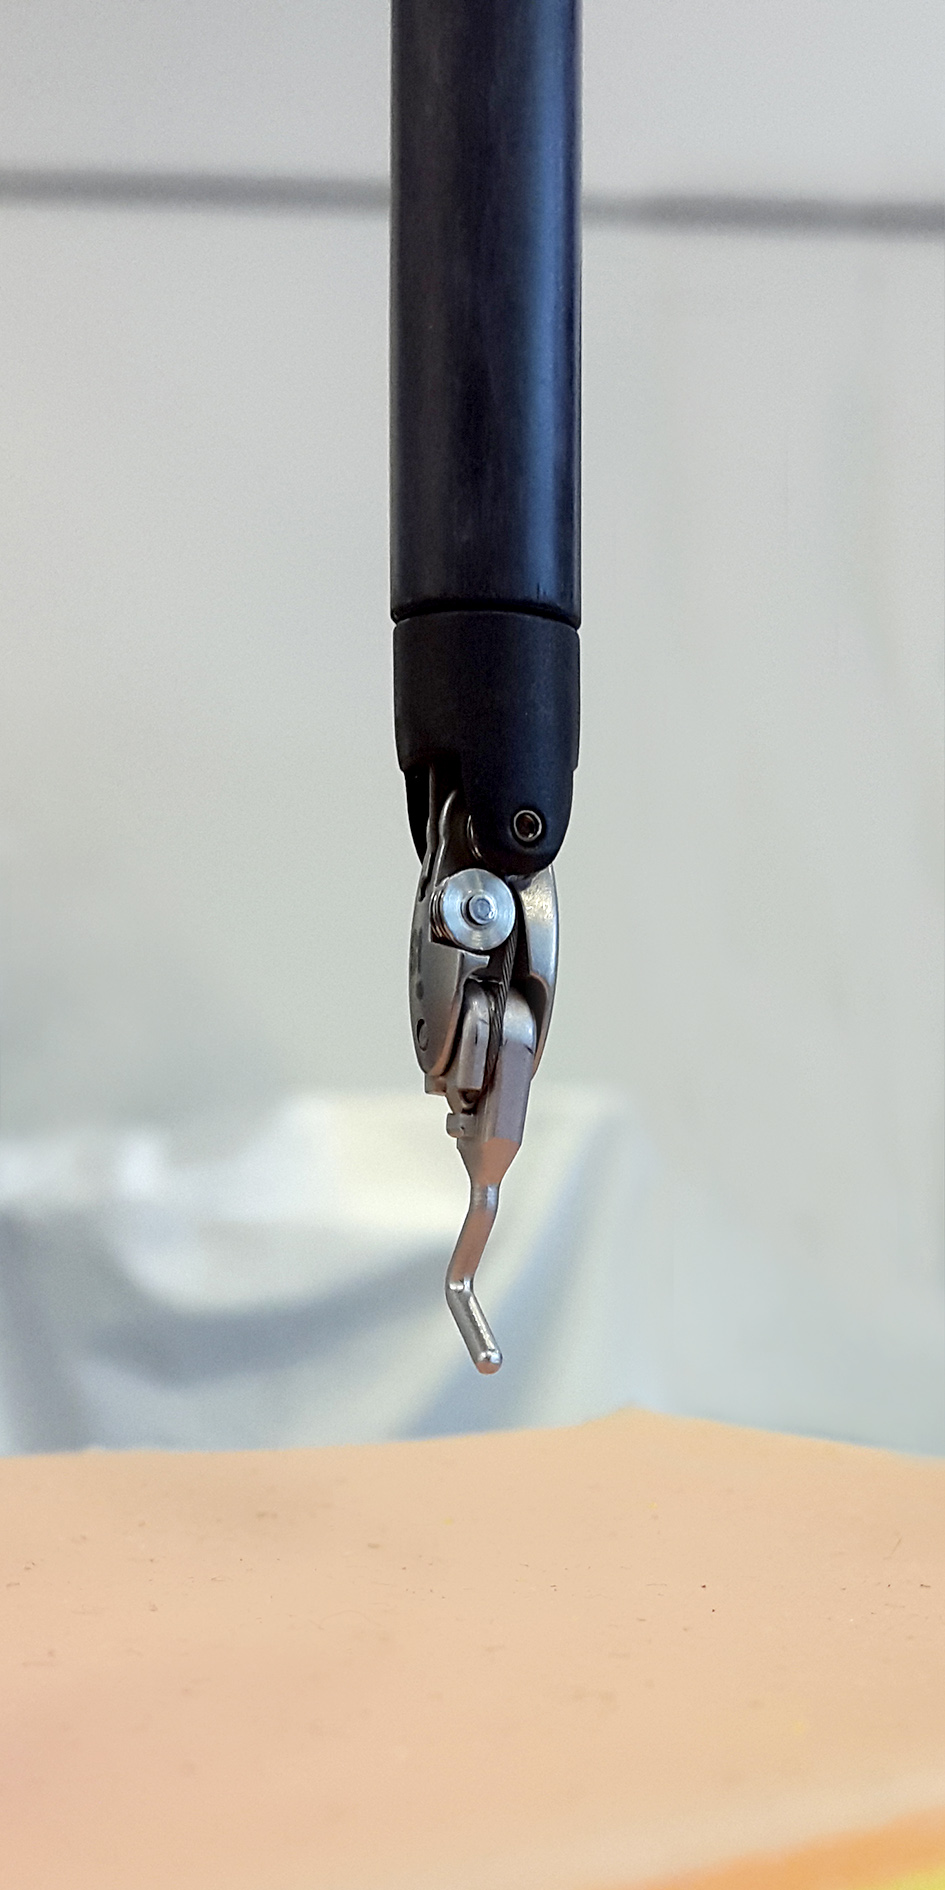
\includegraphics[width=0.23\textwidth]{20150531_171804.jpg}}%
	\caption{Setup of the beating heart implementation. A tissue phantom is mounted on a cylinder controlled by a motor to move as a sinusoid. The robot end effector is following the movement at a distance $d_\text{ref}$.}
	\label{fig:beatingheart_setup}
\end{figure}

The algorithm that implements the beating heart controller is outlined in \autoref{fig:beating_heart_flow}. The developed software can be found in \autoref{app:cd} and in \autoref{app:slide_implement_2}.
The execution time is not shown here as it is verified in \autoref{fig:exe_1} and \autoref{fig:exe_2} that it is far below the allowed maximum execution time and this controller does not constitute heavier calculations. The measured state trajectory is plotted on \autoref{fig:beating_heart_meas}.%


It can from \autoref{fig:beating_heart_meas} be seen how the end effector moves along with the beating heart with a nearly constant distance $d_\text{ref}$. It is seen how the safety controller ensures that $x_1 > x_{h1}$ for all $t$ even when the distance $d_\text{ref}$ is set to the unsafe value -2\,cm. It is also seen how $d_\text{ref}$ can be set to various values. The lack of integral action is again exposed in the plot. It is also seen how the trajectory fluctuates significantly more than the simulated response from \autoref{fig:matlab_dynamics} which is due to the far lower sampling rate.

\begin{figure}[H]
	\center
	\includegraphics[width=1.05\textwidth]{meas_beating_heart.eps}
	\caption{It is seen how $x_1$ moves along with the beating heart with a nearly constant distance $d_\text{ref}$. It is seen how the safety controller ensures that $x_1 > x_{h1}$ for all $t$ even when the distance $d_\text{ref}$ is set to the unsafe value -2\,cm. It is also seen how $d_\text{ref}$ can be set to various values.}
	\label{fig:beating_heart_meas}
\end{figure}

\begin{figure}[H]
	\center
	\includegraphics[width=1\textwidth]{flowchart_beating_controller.pdf}
	\vspace{2mm}
	\caption{Algorithm for dynamic slide safety controller. The source code associated with the algorithm can be found in \autoref{app:slide_implement_2} and in \autoref{app:cd}. It can also be found at github at the Robotic Surgery Group - Aalborg University under the repository \texttt{gr1032} (\textit{https://github.com/AalborgUniversity-RoboticSurgeryGroup/}).}
	\label{fig:beating_heart_flow}
\end{figure}



\vspace{2mm}
\section{Conclusion for the Beating Heart Controller}
\vspace{-1mm}
In conclusion, this chapter verifies that  a control barrier function can be found which indeed ensures safety for the beating heart following  controller, which takes a relative position in the form of the distance to the heart $d_\text{ref}$ as input. It is seen how the developed controller would benefit from a higher sampling rate. It is also seen that the controller suffers from the lack of integral action, and future work on this topic should include integral action as well. 

Finally it is noted that the synchronization of the motor controlled sinusoid movement and the modelled sinusoid implemented on the robot, should be automated for a future test setup through measurements to allow  for model adjustment.
%\newpage
%%\begin{flalign}
%%f_{cl}(x)=\dot{\begin{bmatrix}
%%	x_1\\x_{h1}\\x_{h2}\\d_\text{ref}
%%	\end{bmatrix}} =
%%\underbrace{\underbrace{\begin{bmatrix}
%%		-1/\tau & 0 & 0 & 0\\0 & 0 & \omega_h & 0 \\ 0 & -\omega_h & 0 & 0 \\ 0& 0 & 0 & 0
%%		\end{bmatrix}}_{A}
%%	\begin{bmatrix}
%%	x_1\\x_{h1}\\x_{h2}\\d_\text{ref}
%%	\end{bmatrix}}_{f(x)}+ 
%%\underbrace{\underbrace{\begin{bmatrix}
%%		1/\tau \\ 0 \\ 0 \\ 0
%%		\end{bmatrix}}_{B}}_{g(x)}
%%\underbrace{\underbrace{\begin{bmatrix}
%%		-k & \bar{N} & 0 & \bar{N}
%%		\end{bmatrix}}_{K}
%%	\begin{bmatrix}
%%	x_1\\x_{h1}\\x_{h2}\\d_\text{ref}
%%	\end{bmatrix}}_{\tilde{u}(x)}
%%\end{flalign}
%%or formulated equivalently as
%%\begin{flalign}
%%\dot{\begin{bmatrix}
%%	x_1\\x_{h1}\\x_{h2}
%%	\end{bmatrix}} =
%%\underbrace{\begin{bmatrix}
%%	-(1+k)/\tau & \bar{N}/\tau & 0\\0 & 0 & \omega_h \\ 0 & -\omega_h & 0
%%	\end{bmatrix}}_{A_{cl}}
%%\begin{bmatrix}
%%x_1\\x_{h1}\\x_{h2}
%%\end{bmatrix}+ 
%%\underbrace{\begin{bmatrix}
%%	\bar{N}/\tau \\ 0 \\ 0
%%	\end{bmatrix}}_{B_{cl}}
%%d_{ref}
%%\end{flalign}
%%\begin{tabular}{rl}
%%where &\\
%%$\tau$ & is the time constant of the first order system $\tau=0.11$\,s as given in \autoref{sec:model_slide}\\
%%$k$ & is the linear system controller designed according to \autoref{eq:K_1}\\
%%$\bar{N}$ & is the system gain found according to \autoref{eq:barm_1}
%%\end{tabular}\\
%
%
%
%%
%%where $x_{h1}$ is the position of a point on the surface of the heart and $x_{h2}$ is the velocity of the point.
%%Here $\omega_h$ represents the frequency of the heart, 
%%$\omega_h$ has an average heartbeat period of 1.1\,s \citep{bib:heart_berkeley}, 
%%$\omega_h$ is set to be $2\pi/1.1$. 
%%In \autoref{fig:1stordersys_dynamiclimits} the moving surface of the heart is plotted over time, offset to an axis of oscillation in -6\,cm relative to the slide position. This curve marks the boundary to the unsafe region below it, and crossing this curve (from the safe region above it) corresponds to penetrating the heart surface with the surgical instrument tip. Note that the flexibility of the surface of the heart, at contact with the rigid tool, is not considered in the scope of this thesis. 
%%
%%\begin{figure}[htbp]
%%	\centering
%%	\includegraphics[width=0.65\textwidth]{1stordersys_dynamiclimits.pdf}
%%	\caption{Example of a moving surface representing the heart, marking the boundary to the unsafe region $\mathcal{X}_u$. A reference is set within the safe region as a fixed distance to the surface of the beating heart.}
%%	\label{fig:1stordersys_dynamiclimits}
%%\end{figure}
%%
%%In \autoref{fig:1stordersys_dynamiclimits} a sine amplitude of 2\,cm is used and the time dependent reference for the robot tool tip is defined as the heart position plus a fixed distance of 1\,cm in the positive slide direction $x_\text{ref}=x_{h1}+d_\text{ref}$, i.e. according to \autoref{eq:utilde} the linear position controller to be used in $\mathcal{X}_0$ is
%%\begin{equation}
%%\tilde{u}(t) = \bar{N}(x_{h1}(t)+d_\text{ref})-Kx(t) \label{eq:utilde_dynamic}
%%\end{equation}
%%\textcolor{red}{Or should it be $-k_1x_1$ no matter the order of the system?}
%%The reference distance can be picked as any nonnegative value still allowing the slide position to stay within its (upper) physical limit.
%The dynamic surface representing the heart also put forth new requirements to the safety controller, as the boundary between the safe and unsafe regions $\mathcal{X}_0$ and $\mathcal{X}_u$ (and thereby also the transition region $\mathcal{T}$ between the use of linear and safety controller) is now moving concurrently with the heart surface. This requires the construction of barrier certificates that are functions of robot state as well as the dynamic surface position.
%
%
%
%\section{Safe Controller Design for First Order System}
%First a linear position controller is designed for the augmented system consisting of the first order system modelled in \autoref{subsec:model_1d} and the simplified heart model in \autoref{eq:beating_heart_sine}. The controller is designed on the form presented in \autoref{eq:utilde}, and for the dynamic system, the reference is designed to be a fixed distance to the surface of the heart, as described in \autoref{eq:utilde_dynamic}.
%
%Once the closed-loop system has been designed, a barrier certificate is constructed iteratively by formulating a function that has its (dynamic) zero level set coinciding with the surface position of the heart, and is positive (indicating the unsafe region $\mathcal{X}_u$) below the surface and negative above, thus conforming with the first two requirements for a barrier certificate as given by \autoref{def:barrier_certificate}.
%
%In order to test compliance with the third requirement for a barrier certificate, the candidate barrier function is tested with the designed linear first order system according to the requirement in \autoref{req2}, and the candidate barrier function is altered iteratively until this requirement is fulfilled.
%
%When a barrier certificate for the closed-loop system has been found, a safety controller is designed according to \autoref{eq:control_law_safety}, and the region $\mathcal{T}$ is defined by choosing the constant $\epsilon$ and using the bump function $\sigma(x)$ in \autoref{eq:smoothness}, arriving at the safe controller in \autoref{eq:control_law} employing the linear position controller on $\mathcal{X}_0\setminus\mathcal{T}$ and the linear combination of the position controller and the CBF on $\mathcal{T}$
%
%\subsection{Setting up the Closed-Loop System and Designing the Linear Controller}
%An augmented state-space model including the dynamics of the robot tool from \autoref{eq:1storder_1D_ss} as well as the beating heart from \autoref{eq:beating_heart_sine}, is set up for the closed-loop first order system
%\begin{equation}
%f_{cl}(x)=\dot{\begin{bmatrix}
%	x_1\\x_{h1}\\x_{h2}\\d_\text{ref}
%	\end{bmatrix}} =
%\underbrace{\underbrace{\begin{bmatrix}
%		-1/\tau & 0 & 0 & 0\\0 & 0 & \omega_h & 0 \\ 0 & -\omega_h & 0 & 0 \\ 0& 0 & 0 & 0
%		\end{bmatrix}}_{A}
%	\begin{bmatrix}
%	x_1\\x_{h1}\\x_{h2}\\d_\text{ref}
%	\end{bmatrix}}_{f(x)}+ 
%\underbrace{\underbrace{\begin{bmatrix}
%		1/\tau \\ 0 \\ 0 \\ 0
%		\end{bmatrix}}_{B}}_{g(x)}
%\underbrace{\underbrace{\begin{bmatrix}
%		-k & \bar{N} & 0 & \bar{N}
%		\end{bmatrix}}_{K}
%	\begin{bmatrix}
%	x_1\\x_{h1}\\x_{h2}\\d_\text{ref}
%	\end{bmatrix}}_{\tilde{u}(x)}
%\end{equation}
%or formulated equivalently as
%\begin{equation}
%\dot{\begin{bmatrix}
%	x_1\\x_{h1}\\x_{h2}
%	\end{bmatrix}} =
%\underbrace{\begin{bmatrix}
%	-(1+k)/\tau & \bar{N}/\tau & 0\\0 & 0 & \omega_h \\ 0 & -\omega_h & 0
%	\end{bmatrix}}_{A_{cl}}
%\begin{bmatrix}
%x_1\\x_{h1}\\x_{h2}
%\end{bmatrix}+ 
%\underbrace{\begin{bmatrix}
%	\bar{N}/\tau \\ 0 \\ 0
%	\end{bmatrix}}_{B_{cl}}
%d_{ref}
%\end{equation}
%\begin{tabular}{rl}
%where &\\
%$\tau$ & is the time constant of the first order system $\tau=0.11$\,s as given in \autoref{sec:model_slide}\\
%$k$ & is the linear system controller designed according to \autoref{eq:K_1}\\
%$\bar{N}$ & is the system gain found according to \autoref{eq:barm_1}
%\end{tabular}\\
%
%\textcolor{red}{Should we design a $k$ that is slower conforming with what is found to be implementable?}
%
%Before designing the controller $k$, the stability of this system is analysed. \textcolor{red}{Be sure it's the same for reference as for estimated state!} In order for the system to be (asymptotically) stable, the error should converge to zero
%\begin{equation}
%e(t)=x_\text{ref}(t)-x_1(t)=x_{h1}(t)+d_\text{ref}-x_1(t) = 0 \label{eq:ref_error}
%\end{equation}
%The requirement of the system being stable can be tested as the derivative of the error converging to zero
%\vspace{-5mm}
%\begin{subequations}
%\begin{align}
%\dot{e}(t)=\dot{x}_\text{ref}(t)-\dot{x}_1(t)=\dot{x}_{h1}(t)-\dot{x}_1(t)
%&= \omega_h x_{h2}(t) - (-\tfrac{1}{\tau}x_1(t)+\tfrac{1}{\tau}\bar{N}x_\text{ref}(t-\tfrac{1}{\tau}kx_1(t)) \nonumber\\
%&= \omega_h x_{h2}(t) + \tfrac{1}{\tau}(1+k)x_1(t)-\tfrac{1}{\tau}\bar{N}x_\text{ref}(t)
%\end{align}
%For a first order system of this particular configuration of the $A$ and $B$ matrices, as seen from \autoref{eq:barm_1}, $\bar{N}=1+k$, reducing the equation to
%\begin{equation}
%\dot{e}(t) =\omega_h x_{h2}(t) + \tfrac{1}{\tau}\bar{N}(x_1(t)-x_\text{ref}(t) = \omega_h x_{h2}(t) - \tfrac{1}{\tau}\bar{N}e(t)
%\end{equation}
%Now setting the error derivative equal to zero
%\begin{align}
%0 &= \omega_h x_{h2}(t) - \tfrac{1}{\tau}\bar{N}e(t)\nonumber\\
%\tfrac{1}{\tau}\bar{N}e(t) &= \omega_h x_{h2}(t)\nonumber\\
%e(t) &= \frac{\omega_h \tau}{\bar{N}}x_{h2}(t)
%\end{align}
%The value of $x_{h2}$ is time dependent, but will have its maximum and minimum values in the amplitude of the sine, i.e. for a heart sine amplitude of $A_\text{heart}=2$\,cm $x_{h2}\in[-0.02,0.02]$\,m.
%\end{subequations}
%This means that the error will fluctuate between the values
%\begin{equation}
%e(t) \in \begin{bmatrix} -\frac{\omega_h \tau}{\bar{N}}A_\text{heart},  & \frac{\omega_h \tau}{\bar{N}}A_\text{heart}  \end{bmatrix}
%\end{equation}
%\textcolor{red}{Makes no sense! How can the error derivative be zero only when the error is fluctuating?!}
%From safety, $x_1$ should always be above $x_{h1}$, i.e.
%\begin{equation}
%x_1(t)\geq x_{h1}(t) \qquad \Leftrightarrow \qquad x_{h1}(t)-x_1(t)\leq 0
%\end{equation}
%and as seen from \autoref{eq:ref_error}, this puts up a safety requirement for the reference distance
%\begin{equation}
%x_{h1}(t)-x_1(t) = e(t)-d_\text{ref}\leq 0 \qquad \Leftrightarrow \qquad d_\text{ref}\geq e_\text{max}=\frac{\omega_h \tau}{\bar{N}}A_\text{heart}
%\end{equation}
%
%Stability analysis: test that the system has negative poles, i.e. that all $\lambda$s are negative for which
%\begin{equation}
%\det\begin{vmatrix}
%A_{cl}-\lambda I & B_{cl}\\C_{cl}&D_{cl}
%\end{vmatrix}=0
%\end{equation}
%As the output should be the robot tool position, i.e. $C_{cl}=[1\,\,\,0\,\,\,0]$ and $D_{cl}=0$, this is found as
%\begin{align}
%&\det\begin{vmatrix}
%-(1+k)/\tau-\lambda & \bar{N}/\tau & 0 & \bar{N}/\tau\\
%0 & -\lambda  & \omega_h  & 0\\ 
%0 & -\omega_h & -\lambda & 0\\
%1 & 0 & 0 & 0
%\end{vmatrix}
%= 
%%(-(1+k)/\tau-\lambda) \cdot
%%\begin{vmatrix}
%%-\lambda  & \omega_h  & 0\\ 
%%-\omega_h & -\lambda & 0\\
%%0 & 0 & 0
%%\end{vmatrix}
%-1 \cdot \det\begin{vmatrix}
%\bar{N}/\tau & 0 & \bar{N}/\tau\\
%-\lambda & \omega_h  & 0\\ 
%-\omega_h & -\lambda & 0\\
%\end{vmatrix} \nonumber\\
%&\phantom{det}= -1\cdot \frac{\bar{N}}{\tau} \cdot \det 
%\begin{vmatrix}
%-\lambda & \omega_h\\
%-\omega_h &  -\lambda\\
%\end{vmatrix}
%= -\frac{\bar{N}}{\tau} \cdot (\lambda^2 +\omega_h^2)
%= 0 \qquad \Leftrightarrow \qquad \lambda = \pm\omega_h
%\end{align}
%\textcolor{red}{Not stable! positive eigenvalue in $\omega_h$}
%
%\subsection{Constructing a Control Barrier Function}
%As mentioned, a barrier certificate for this system with a zero level set at the surface of the heart, comprises moving boundaries and hence should be a function of both robot and heart position. According to \autoref{def:safety} a $B(x_1,x_{h1})$ should be constructed with unsafe region $\mathcal{X}_u$ below the surface of the heart, i.e. such that $B(x_1,x_{h1})$ is positive if $x_1<x_{h1}$ and negative otherwise. The very simplest function satisfying this requirement is a function
%\begin{equation}
%B_0(x_1,x_{h1})= c(x_{h1}-x_1)
%\end{equation}
%with a positive constant $c>0$. This would result in the Lie derivatives % $L_{f_{cl}}B_0(x)$
%\begin{subequations}
%\begin{align}
%L_fB_0(x) &= \frac{dB_0(x)}{dx}f(x) =
%\begin{bmatrix}
%-c & c & 0 & 0
%\end{bmatrix}
%\begin{bmatrix}
%-x_1/\tau\\
%\omega_h x_{h2} \\
%-\omega_h x_{h1} \\
%0
%\end{bmatrix}=
%c\left(\omega_h x_{h2} + \frac{ x_1}{\tau}\right)\\
%L_gB_0(x) &= \frac{dB(x)}{dx}g(x) =
%\begin{bmatrix}
%-c & c & 0 & 0
%\end{bmatrix}
%\begin{bmatrix}
%1/\tau\\
%0 \\ 0 \\ 0
%\end{bmatrix}=
%\frac{-c}{\tau}\\
%L_{f_{cl}}B_0(x) & 
%%=\frac{dB_0(x)}{dx}f_{cl}(x) 
%= L_fB_0(x)+L_gB_0(x)u = 
%%\begin{bmatrix}
%%	-c & c & 0 & 0
%%\end{bmatrix}
%%\begin{bmatrix}
%%\frac{\bar{N}(x_{h1}+d_{ref})-(1+k) x_1}{\tau} \\
%%\omega_h x_{h2} \\
%%-\omega_h x_{h1}
%%\end{bmatrix}=
%c\left(\omega_h x_{h2} - \frac{\bar{N}(x_{h1} + d_{ref})-(1+k) x_1}{\tau}\right)
%\end{align}
%\end{subequations}
%The Lie derivative $L_{f_{cl}}B_0(x)$ (with the heart sine placed as in \autoref{fig:1stordersys_dynamiclimits}) should be negative for  $x_1\in[-0.1,0.1]$, $x_{h1}\in [-0.08,-0.04]$ and $x_{h2}\in [-0.02,0.02]$. We thus require that (recall from \autoref{eq:barm_1} that $\bar{N}=K+1$ for the present first order system)
%\begin{align}
%\omega_h x_{h2} &< \frac{\bar{N}(x_{h1} + d_{ref})-(1+k) x_1}{\tau} = \frac{1+k}{\tau}(x_{h1} + d_{ref}-x_1)\nonumber\\
%\omega_h x_{h2} \frac{\tau}{1+k} &< x_{h1} + d_{ref}-x_1
%\end{align}
%With the largest positive value of $x_{h2}=0.02$\,m and the same controller $K=9$ is used as in \autoref{eq:K_1}, the left-hand expression attains a largest value of 0.00126\,m, requiring that the error between the robot tool position and the reference position always be slightly larger than a millimeter. 
%%2*pi/1.1*0.02/(10/0.11)
%%0.001256637061436
%Obviously this barrier function is not valid, and a different function is opted for.
%
%According to \cite{bib:org_control} a barrier certificate might be found iteratively by using $B_0(x)$ in the construction of a barrier certificate on the form
%\begin{equation}
%B(x) = 
%\begin{cases}
%B_0(x) & \text{if}\quad L_fB_0(x) \leq -\beta\\
%B_0(x)+\alpha(L_fB_0(x)+\beta)^2 & \text{if}\quad L_fB_0(x)>-\beta 
%\end{cases}
%\end{equation}
%where $\alpha>0$, $\beta>0$ are parameters to be determined. For the presented system this gives the barrier candidate function 
%\begin{equation}
%B(x) = 
%\begin{cases}
%c(x_{h1}-x_1) & \text{if}\quad c\left(\omega_h x_{h2} +  x_1/\tau\right) \leq -\beta\\
%c(x_{h1}-x_1)+\alpha(c\left(\omega_h x_{h2} +  x_1/\tau\right)+\beta)^2 & \text{if}\quad c\left(\omega_h x_{h2} +  x_1/\tau\right)>-\beta 
%\end{cases}
%\end{equation}
%\textcolor{red}{The constant $c$ is unimportant. Set $c=1$.  In the example in \citep{bib:org_control} they chose $\alpha=1/20$ and $\beta=1$, giving}
%\begin{equation}
%B(x) = 
%\begin{cases}
%x_{h1}-x_1 & \text{if}\quad x_1 \leq -0.11-0.2\pi x_{h2}\\
%x_{h1}-x_1+\dfrac{1}{20}\left(\dfrac{0.2\pi\,\, x_{h2} +   x_1}{0.11}+1\right)^2 & \text{if}\quad x_1 > -0.11-0.2\pi x_{h2} 
%\end{cases}
%\end{equation}
%\textcolor{red}{Need to test this!}
%
%
%\section{Safe Controller Design for Second Order System}
%\textcolor{red}{introduce}
%
%\subsection{Setting up the Closed-Loop System and Designing the Linear Controller}
%As for the first order system, the second order system in \autoref{eq:2ndorder_1D_ss} is augmented with the dynamics of the beating heart and with the reference given as a fixed distance from the surface of the beating heart
%\begin{equation}
%\dot{\begin{bmatrix}
%x_1\\x_2\\x_{h1}\\x_{h2}
%\end{bmatrix}} = \begin{bmatrix}
%0 & 1 & 0 & 0\\
%-\omega_n^2(1+k_1)  & -2\zeta \omega_n-\omega_n^2 k_2  & \omega_n^2\bar{N} & 0\\
%0 & 0 & 0 & \omega_h \\
%0 & 0 & -\omega_h & 0
%\end{bmatrix}\begin{bmatrix}
%x_1\\x_2\\x_{h1}\\x_{h2}
%\end{bmatrix} + \begin{bmatrix}
%0\\\omega_n^2\bar{N} \\ 0 \\ 0
%\end{bmatrix}d_{ref}
%\end{equation}
%\begin{tabular}{rl}
%where &\\
%$\omega_n$ & is the natural frequency of the second order system $\omega_n=17$\,rad/s as given in \autoref{sec:model_slide}\\
%$\zeta$ & is the damping ratio of the second order system $\zeta=0.05$ as given in \autoref{sec:model_slide}\\
%$[k_1\,\,\,k_2]$ & is the linear system controller designed according to \autoref{eq:K_2}\\
%$\bar{N}$ & is the system gain found according to \autoref{eq:Nbar_2}
%\end{tabular}\\
%
%
%Can also be written on augmented form where the reference is part of the state
%\begin{equation}
%\dot{\begin{bmatrix}
%	x_1\\x_2\\x_{h1}\\x_{h2}\\d_{ref}
%	\end{bmatrix}} = 
%\underbrace{\underbrace{\begin{bmatrix}
%		0 & 1 & 0 & 0 & 0\\
%		-\omega_n^2  & -2\zeta \omega_n  & 0 & 0 & 0\\
%		0 & 0 & 0 & \omega_h & 0\\
%		0 & 0 & -\omega_h & 0 & 0\\
%		0 & 0 & 0 & 0 & 0
%		\end{bmatrix}}_{A}
%	\begin{bmatrix}
%	x_1\\x_2\\x_{h1}\\x_{h2}\\d_{ref}
%	\end{bmatrix}}_{f(x)} + 
%\underbrace{\underbrace{\begin{bmatrix}
%		0\\\omega_n^2 \\ 0 \\ 0 \\ 0
%		\end{bmatrix}}_{B}}_{g(x)}
%\underbrace{\underbrace{\begin{bmatrix}
%		-k_1 & -k_2 & \bar{N} & 0 & \bar{N}
%		\end{bmatrix}}_{K}
%	\begin{bmatrix}
%	x_1\\x_2\\x_{h1}\\x_{h2}\\d_{ref}
%	\end{bmatrix}}_{u}
%\end{equation}
\chapter{Extending Safety\,to\,the\,Euclidean Space}\label{chap:cbf_3d_static}
This chapter presents the design of a safe controller for the  robotic patient manipulator in 3D Cartesian space, where the unsafe region is defined as an ellipsoid with static boundaries, i.e. fixed in space with respect to time. The unsafe region is defined such that it is within the reach of the instrument tip. 

The robotic patient manipulator constitutes four "arms" (see \autoref{fig:master-slave_surgery}) each comprising a number of arm links, whose joints are fixed by electromagnets that are manually released for positioning of these links; followed by the robot "hand" and instrument links, whose joints are available for automated control on the modified AAU da Vinci robot. Only the controllable part of the robotic patient manipulator, as displayed in \autoref{fig:robot_hand_3d}, is considered in the design of the 3D Cartesian space controller. 

\begin{figure}[htbp]
\centering
\subbottom[Robotic patient manipulator.]{\includegraphics[width=0.45\textwidth]{rviz_09_17_18_frame1.pdf}\label{fig:rviz_09_17_18_frame}}%
	\hspace*{5mm}
\subbottom[Robotic "hand" and instrument.]{\includegraphics[width=0.45\textwidth]{robot_hand_unsafe_region.pdf}\label{fig:robot_hand_unsafe_region}}%
\caption{Patient manipulator and a fixed region within the reachable space $\mathcal{X}$ that is unsafe, $\mathcal{X}_u$, marked by a red ellipsoid.}
\label{fig:robot_hand_3d}
\end{figure}

The controller is designed for and tested on the da Vinci robot comprising the prismatic slide joint as described in \autoref{chap:cbf_1d_static} as well as five independent revolute joints. In order to design a controller in 3D Cartesian space for the robot, a kinematic description of the robot links and joints is necessary as a translation between the 3D Cartesian space and the 6D joint space.
Hence, before modelling the system and designing a controller, the kinematics of the AAU da Vinci robot is presented in the following section along with considerations for the definition of the coordinate frames and the transformation between them constituting the kinematic description of the robot.


\section{Kinematics of the AAU da Vinci Robot}
A kinematic description of an object requires defining a right-handed coordinate frame fixed in the object and a coordinate frame fixed in inertial space, the latter which the position and orientation of the object can be described relative to. This relative orientation and position of an object (or the frame $i$ fixed in it) with respect to another frame $j=i-1$ can be described through a transformation matrix $T$, containing the orthonormal rotation matrix $R$ and the translation vector $p$ of the frame origin, as 
\begin{equation}
^j_iT = 
\begin{bmatrix}
^j_iR & ^j_ip\\
0 & 1
\end{bmatrix}, \label{eq:kin_transformation}
\qquad \text{where} \qquad
^j_ip = 
\begin{bmatrix}
a\\b\\d
\end{bmatrix}
\end{equation}
and the simplest rotation matrices $R$ are rotations about a single axis, which can be combined to obtain an arbitrary rotation
\begin{small}
	\begin{equation}
	R_x(\alpha) = 
	\begin{bmatrix}
	1 & 0 & 0\\
	0 & \cos\alpha & -\sin\alpha\\
	0 & \sin\alpha & \cos\alpha
	\end{bmatrix} 
	\qquad
	R_y(\beta) = 
	\begin{bmatrix}
	\cos\beta & 0 & \sin\beta \\
	0 & 1 & 0\\
	-\sin\beta & 0 & \cos\beta
	\end{bmatrix}
	\qquad
	R_z(\theta) = 
	\begin{bmatrix}
	\cos\theta & -\sin\theta & 0\\
	\sin\theta & \cos\theta & 0\\
	0 & 0 & 1
	\end{bmatrix}
	\label{eq:RxRyRz_chapter}
	\end{equation}
\end{small}

For the robotic patient manipulator comprising a number of links, coordinate frames are defined for each degree of freedom, i.e. placed in each joint such that one of the frame axes is the axis of free rotation or translation. The kinematic chain is now the sequence of alternate links and joints starting from the link fixed in inertial space and ending at the tip of the robotic tool. The link preceding a joint is its parent link, while the link succeeding it is its child link. The transformation between any two frames is given as the product of the transformation matrices in the kinematic chain between them. An example of a sequence of transformations can be seen in \autoref{app:kinematic_model_robot}.

For the resolution of frame definitions it is preferred to adapt the  robot coordinate frame convention \gls{dh} because it is one of the most widespread kinematic descriptions in the robot kinematics community, and because it describes transformations between two successive frames in the kinematic chain on a succinct and standardized form
\begin{equation}
\hspace*{-2mm}
\small
^{i-1}_{\phantom{-1}i} T =
\begin{bmatrix}
R_z(\theta_i) & \begin{bmatrix}0\\ 0\\ d_i\end{bmatrix}\\
0 & 1
\end{bmatrix}
\begin{bmatrix}
R_x(\alpha_i) & \begin{bmatrix}a_i\\ 0\\ 0\end{bmatrix}\\
0 & 1
\end{bmatrix}
\label{eq:dh}
\end{equation}
In the \gls{dh} kinematic description each frame is fixed with respect to its parent link, and its $z$-axis is aligned with the actuation axis of its child link. The free rotation/translation always taking place around/along the local $z$ axis, and as seen from \autoref{eq:dh} any fixed or free rotation/translation about/along the $z$-axis is implemented (intrinsically) before any fixed rotation/translation about/along the (new) $x$-axis. For more details on the \gls{dh} convention and robot frames defined according to is, see \autoref{sec:denavit_hartenberg}.

%\begin{itemize}
%	\itemsep-1.3mm 
%	\item variable/parameter $\theta_i$ is the angle from $x_{i-1}$ to $x_i$ about $z_{i-1}$
%	\item variable/parameter $d_i$ is the distance from origin $i-1$ to $x_i$ measured along $z_{i-1}$
%	\item parameter $a_i$ is the distance from $z_{i-1}$ to $z_i$ measured along $x_i$
%	\item parameter $\alpha_i$ is the angle from $z_{i-1}$ to $z_i$ about $x_i$
%\end{itemize}

In the robot description in \gls{ros}, however, the kinematics are described in the \texttt{xacro} files on the form
\begin{equation}
\hspace*{-2mm}
\small
^{i-1}_{\phantom{-1}i}T =
\begin{bmatrix}
R_z(\text{yaw})R_y(\text{pitch})R_x(\text{roll}) & \begin{bmatrix}a_i\\ b_i\\ d_i\end{bmatrix}\\
0 & 1
\end{bmatrix}
\begin{bmatrix}
R_z(\theta_i^*)R_y(\beta_i^*)R_x(\alpha_i^*) & \begin{bmatrix}a_i^*\\ b_i^*\\ d_i^* \end{bmatrix}\\
0 & 1
\end{bmatrix}
\label{eq:xacro_transformation_chapter}
\end{equation}
Here fixed translations are implemented first, then RPY rotations (extrinsic roll (about $x$-axis), pitch (about $y$-axis), yaw (about $z$-axis) rotation), and finally the free rotation or translation (denoted by $^*$ in \autoref{eq:xacro_transformation_chapter}) about/along one of the rotated axes. Furthermore, the convention here is that each frame (joint) is fixed in its child link (corresponding to the fixed rotations preceding the free rotation), and not in its parent link as in the DH convention. The transformation  $^{i-1}_{\phantom{-1}i} T$ is implemented in joint $i$ in the \texttt{xacro} file  as (for joint 8)
\begin{lstlisting}[language=xml]
<joint name="p4_hand_pitch"  type="revolute">
<origin
xyz="0 0 0"
rpy="1.5708 0 0" />
<parent link="rcm_vitual0" />
<child link="rcm_vitual1" />
<axis xyz="0 0 1" />
...
</joint>
\end{lstlisting}

A compromise is made, defining a new set of frames for the da Vinci kinematics, adhering to the \gls{dh} constraint that each free rotation/translation is about/along the local $z$-axis. The new kinematic frames are visualized in \autoref{fig:p4_hand_compromise_frames_chapter}, the parameters listed in table \ref{tab:new_kin_short}. Furthermore, for simplification of the inverse kinematics solver, the two passive joints mimicking the hand pitch movement are removed from the existing kinematic chain, visualized in \autoref{fig:p4_hand_xacro_frames_chapter}, and parameters listed in table \ref{tab:old_kin_short} for comparison.  



\begin{table}[htbp]
	\small
	\centering
\subbottom[Old robot hand kinematics including mimicking joints, corresponding to \autoref{fig:p4_hand_xacro_frames_chapter}.]{%
	\begin{tabular}{r | rrr | ccc | c l}\hline
		& \multicolumn{3}{c|}{fixed translation  [m]} & \multicolumn{3}{c|}{fixed rotation [rad]} & freedom & \\
		frame  & $a$ ($x$)  & $b$ ($y$)  & $d$ ($z$)  & roll  & pitch & yaw & $\alpha^*, \beta^*, \theta^*$ or $d^*$ & joint name\\\hline
		7 & -0.042 & 0 & 0.161 & 0 & 0 & 0 & $\phantom{-}\alpha_7^*$ & \texttt{hand\_roll} \\
		8 & 0 & 0 & 0 & 0 & -0.288 & 0 & $-\beta_8^*$ & \texttt{hand\_pitch} \\
		9 & 0.011 & 0 & 0.186 & $\pi$ & 0.288 & 0 & $\phantom{-}\beta_8$ & mimic \texttt{hand\_pitch} \\
		10 & 0.520 & 0 & 0 & $\pi$ & 0& 0 &  $-\beta_8$ & mimic \texttt{hand\_pitch} \\
		11 & 0 & 0 & -0.120  & 0 & 0 & 0 & $\phantom{-}d_{11}^*$ & \texttt{instrument\_slide} \\
		12 & 0.052 & 0 & 0 & $\pi$ & 0 & $\pi/2$ & $\phantom{-}\theta_{12}^*$ & \texttt{instrument\_roll} \\
		13 & 0 & 0 & 0.177 & 0 & 0 & 0 & $-\alpha_{13}^*$ & \texttt{instrument\_pitch} \\
		14L & 0 & 0 & 0.009 & $\pi/2$ & $\pi/2$ & 0 & $-\theta_{14L}^*$ & \texttt{instrument\_jaw\_left} \\
		14R & 0 & 0 & 0.009 & $\pi/2$ & $\pi/2$ & 0 & $\phantom{-}\theta_{14R}^*$ & \texttt{instrument\_jaw\_right} \\
	\end{tabular}\label{tab:old_kin_short}}
	\vspace*{1mm}
\subbottom[New robot hand kinematics excluding mimicking joints, corresponding to \autoref{fig:p4_hand_compromise_frames_chapter}.]{%
	\begin{tabular}{r | rrr | ccc | c l}\hline
		& \multicolumn{3}{c|}{fixed translation  [m]} & \multicolumn{3}{c|}{fixed rotation [rad]} & freedom & \\
		frame  & $a$ ($x$)  & $b$ ($y$)  & $d$ ($z$)  & roll  & pitch & yaw & $\theta^*$ or $d^*$ & joint name\\\hline
		7 & 0.482 & 0 & 0.047 & 0 & $\pi/2$ & 0 & $\theta_7^*$ & \texttt{hand\_roll} \\
		8 & 0 & 0 & 0 & $\pi/2$ & 0 & 0 & $\theta_8^*$ & \texttt{hand\_pitch} \\
		9 & 0.097 & 0 & 0 & 0 & $-\pi/2$ &  0 & $d_9^*$ & \texttt{instrument\_slide} \\
		10 & 0 & 0 & 0 & 0 & 0 & 0 & $\theta_{10}^*$ & \texttt{instrument\_roll} \\
		11 & 0 & 0 & 0 & 0 & $\pi/2$ & 0 & $\theta_{11}^*$ & \texttt{instrument\_pitch} \\
		12L & 0.009 & 0 & 0 & $-\pi/2$ & 0 & 0 & $\theta_{12L}^*$ & \texttt{instrument\_jaw\_left} \\
		12R & 0.009 & 0 & 0 & $-\pi/2$ & 0 & 0 & $\theta_{12R}^*$ & \texttt{instrument\_jaw\_right} \\
		\end{tabular}\label{tab:new_kin_short}}
	\caption{Parameters and variables (marked with $^*$) for the robot kinematic description implemented in \gls{ros} and visualized in \autoref{fig:robot_hand_kinematics}. Free angles are named with $\alpha$ being a rotation about the $+x$-axis, $\beta$ about the $+y$-axis and $\theta$ about the $+z$-axis.}
	\label{tab:xacro_param_short}
\end{table}



\begin{figure}[htbp]
\hspace*{-15mm}
\begin{minipage}{1.15\textwidth}
	\subbottom[Old robot hand kinematics including mimick joints, parameters given in table \ref{tab:old_kin_short}.]{\includegraphics[width=\textwidth]{p4_hand_xacro_frames_chapter.pdf}\label{fig:p4_hand_xacro_frames_chapter}}%
	\vspace*{5mm}
	\subbottom[New robot hand kinematics excluding mimick joints, parameters given in table \ref{tab:new_kin_short}.]{\includegraphics[width=\textwidth]{p4_hand_compromise_frames_chapter.pdf}\label{fig:p4_hand_compromise_frames_chapter}}%
	\caption{Orientation and position of coordinate frames $\Psi_7$, $\Psi_8$, etc. corresponding to the controllable joints of the robotic patient manipulator.  For convenience of placing the hand roll and pitch frames in the pivot point in the new kinematic description in \autoref{fig:p4_hand_compromise_frames_chapter}, a virtual link is inserted in the \texttt{xacro} file after each of these two joints.}
	\label{fig:robot_hand_kinematics}
\end{minipage}
\end{figure}
For more details on the original and new kinematic descriptions implemented in \gls{ros}; including all measurements of parameters, gearing ratios, code for testing the kinematic description in Matlab, and measurements of distances for different configurations; please refer to \autoref{sec:existing_kinematics} and \ref{sec:app_activejoints_kinematics} in \autoref{app:kinematic_model_robot}.










\subsection{Employing Inverse Kinematics for a Controller in 3D Cartesian Space}
The controller presented in this chapter is developed for 3D position and orientation control of the tool tip, and hence relies on the use of inverse kinematics for the (ambiguous) mapping from 3D Cartesian space to 6D joint space. The inverse of the kinematic transformation matrix presented in \autoref{eq:kin_transformation} is
\begin{equation}
^j_iT^{-1} = 
\begin{bmatrix}
^j_iR^T & -^j_iR^T\,\,^j_ip\\
0 & 1
\end{bmatrix}
\end{equation}
With the sequence of transformations from frame $k$ to frame $i$ being represented by the transformation matrix $^k_i T$, the inverse transformation, from frame $i$ to frame $k$, is then its matrix inverse $^k_i T^{-1}$
\begin{equation}
^k_iT = ^k_jT \,\, ^j_iT =
\begin{bmatrix}
^k_jR \,\, ^j_iR & ^k_jp+^k_jR \,\, ^j_ip\\
0 & 1
\end{bmatrix}
\qquad \Leftrightarrow \qquad
^k_iT^{-1} = 
\begin{bmatrix}
^j_iR^T\,\, ^k_jR^T & -\,^j_iR^T\,\, ^k_jR^T\,\,^k_jp -\, ^j_iR^T\,\, ^j_ip\\
0 & 1
\end{bmatrix}
\end{equation}
A mapping from six to three degrees of freedom is a surjective map, i.e. several elements in the 6D domain may map to the same element in the 3D co-domain. However the inverse map from 3D to 6D is neither injective nor surjective, as each element in the 3D domain can map to several elements in the 6D co-domain, and hence the mapping requires a decision of the "best" map.

In practice this mapping from the desired 3D Cartesian space configuration to a prudent 6D joint space position of the da Vinci robotic patient manipulator is handled by the \gls{kdl} inverse kinematics solver. Then the transformed joint position commands are passed to the low level controllers (see \autoref{fig:overview}).

The \gls{ik} \gls{kdl} solver employed in \gls{ros} utilizes the kinematic chain from the URDF, which is generated from the \texttt{xacro} link and joint kinematic description as presented in %\autoref{app:kinematic_model_robot}, the model implemented in ROS defined in
\autoref{sec:app_activejoints_kinematics}. From this chain (\texttt{my\_chain} in the below example) a \gls{fk} position solver is created along with an \gls{ik} velocity solver in order to define the \gls{ik} position solver:

\begin{lstlisting}[language=xml]
//Create solver based on kinematic chain
KDL::ChainFkSolverPos_recursive fksolver(my_chain);
KDL::ChainIkSolverVel_pinv iksolverv(my_chain);
KDL::ChainIkSolverPos_NR iksolver = KDL::ChainIkSolverPos_NR(my_chain,fksolver,iksolverv,100,1e-6);

KDL::JntArray q(my_chain.getNrOfJoints());
KDL::JntArray q_init(my_chain.getNrOfJoints());

//Set destination frame
double x, y, z;
std::cout << "Set end-effector position <x y z>:" << std::endl;
std::cin >> x >> y >> z;
KDL::Vector dest_pos(x,y,z);
KDL::Frame dest_frame(dest_pos);

// Compute!
int ret = iksolver.CartToJnt(q_init,dest_frame,q);
\end{lstlisting}

The \gls{kdl} \gls{ik} position solver uses the Newton-Raphson iterative numerical technique through the function \texttt{CartToJnt} to determine a prudent joint configuration implementing the desired Cartesian configuration (given as \texttt{dest\_frame} in the above example). In the above example the initial guess \texttt{q\_init} of the joint configuration is the current joint configuration, and hence care should be taken to only command small changes in configuration for the sake of fast convergence of the \gls{ik} solution.


Three dimensional positions of the tool tip is described in a frame oriented as the inertial frame and offset such that a robot configuration with all free angles and slide set to zero equals a position of the tool tip in [0,0,0].




\section{Modelling of Robot Hand Movement in 3D}
In order to set up a dynamic model of the da Vinci robot hand, a decision is made to model the three axes as decoupled for initial simplification. \textcolor{red}{Argue why, something about measurement, as movements are composed from changing joint angles obviously the axes are coupled, but it is also dependent on the low level controllers on the FPGA.} Measurements are made for a step input on each of the three axes, as shown in \textcolor{red}{FIGURE}

\textcolor{red}{Make measurement of step for cases: x-axis, y-axis, z-axis, and xyz at the same time. Compare to slide measurement.}

It is decided to model the response for each of the three (decoupled) axes as three first order systems, and the open loop system for the robot hand is formulated as:
\begin{equation}\label{eq:3D_sys_static_openloop}
\dot{\mathbf{x}}=
\dot{\begin{bmatrix}
x_x\\x_y\\x_z
\end{bmatrix}} =
\underbrace{\begin{bmatrix}
-1/\tau_x & 0 & 0\\0 & -1/\tau_y & 0 \\ 0 & 0 & -1/\tau_z
\end{bmatrix}
\begin{bmatrix}
x_x\\x_y\\x_z
\end{bmatrix}}_{f(\mathbf{x})} +
\underbrace{\begin{bmatrix}
1/\tau_x& 0 & 0 \\ 0& 1/\tau_y & 0 \\0& 0& 1/\tau_z
\end{bmatrix}}_{g(\mathbf{x})}
\mathbf{u}(\mathbf{x})
\end{equation}
with time constant from \textcolor{red}{MEASUREMENT}

\section{Construction of CBF}
A candidate barrier certificate is proposed that complies with the first two constraints in \autoref{def:barrier_certificate}, i.e. a function that is positive on the set $\mathcal{X}_u$ and nonpositive on the set $\mathcal{X}_0$. In order to make sure that the robot tool will not penetrate the heart, the unsafe set $\mathcal{X}_u$ is defined as an ellipsoid representing the heart. This ellipsoid enclosing the region $\mathcal{X}_u$ as visualized in \autoref{fig:robot_hand_unsafe_region}, must be the zero level set of the candidate CBF. A candidate CBF is proposed of the form:
\begin{equation}
	B_0(\mathbf{x}) = -\left(  \left(\frac{x_x-c_x}{r_x}\right)^2 + \left(\frac{x_y-c_y}{r_y}\right)^2 + \left(\frac{x_z-c_z}{r_z}\right)^2 - 1 \right)\label{eq:barrier_3d}
\end{equation}
\begin{tabular}{rl}
	where&\\
	$[c_x\,\, c_y\,\, c_z]$ & is the coordinate of the center of the ellipsoid, $\mathbf{c}\in\mathbb{R}^3$ \\
	$[r_x\,\, r_y\,\, r_z]$ & is the lengths of the semi-axes of the ellipsoid, $\mathbf{r}\in\mathbb{R}^3_+$, an average heart size is [12,6,8]\,cm\\
\end{tabular}\\

\textcolor{red}{Where should we define the center of the ellipsoid - should be such that the tool can reach all the way around it (but not necessarily below)}

An example of a function of this form is visualized in \autoref{fig:zerolevelset_3d}, the zero level set enclosing the unsafe region $\mathcal{X}_u$ shown as a red ellipsoid, the one level set shown in black. Note that the function $-B(\mathbf{x})$ will have the same zero level set, but have positive values outside the ellipsoid, indicating that it is the safe area $\mathcal{X}_0$ that is enclosed by the ellipsoid.

\begin{figure}[htbp]
	\centering
	\hspace*{-15mm}
	\includegraphics[width=0.7\textwidth]{zerolevelset_3d.pdf}
	\caption{Example of a CBF on the form described in \autoref{eq:barrier_3d}, here with $\mathbf{c}= [0.1,\,\,\,\, 0,\,\,\,\, -0.05]$ and $\mathbf{r}=[0.2,\,\,\,\, 0.1,\,\,\,\, 0.1]$. The zero level set is indicated by the red ellipsoid, while the black ellipsoid marks the one level set, indicating that the enclosed  region is the unsafe set $\mathcal{X}_u$).}
	\label{fig:zerolevelset_3d}
\end{figure}

The third constraint in \autoref{def:barrier_certificate} is tested for a barrier certificate of this form with the system in \autoref{eq:3D_sys_static_openloop}. This is done by splitting the constraint up into the combined constraints on $L_gB(\mathbf{x})$ and $L_fB(\mathbf{x})$ from \autoref{req2}, first testing where $L_gB_0(\mathbf{x})=0$:
\begin{align}
	L_gB_0(\mathbf{x}) = \frac{dB_0(\mathbf{x})}{d\mathbf{x}}g(\mathbf{x}) &= 
	\begin{bmatrix} 
		\frac{2}{r_x^2}(c_x-x_x) & \frac{2}{r_y^2}(c_y-x_y) & \frac{2}{r_z^2}(c_z-x_z) 
	\end{bmatrix}
	\begin{bmatrix}
		1/\tau_x& 0 & 0 \\ 0& 1/\tau_y & 0 \\0& 0& 1/\tau_z
	\end{bmatrix} \nonumber\\
	&= 2
	\begin{bmatrix} 
		\frac{1}{r_x^2\tau_x}(c_x-x_x) & \frac{1}{r_y^2\tau_y}(c_y-x_y) & \frac{1}{r_z^2\tau_z}(c_z-x_z) 
	\end{bmatrix}
\end{align}
It can be seen that $L_gB(\mathbf{x})=0$ in the centre of the ellipsoid $[c_x,c_y,c_z]$, which is the vertex of the barrier function. This means that instead of testing $L_fB(\mathbf{x})<0$ in this point, the relaxed requirement $L_fB(\mathbf{x})\leq 0$ applies:
\begin{align}
	L_fB_0(\mathbf{x}) &= \frac{dB_0(\mathbf{x})}{d\mathbf{x}}f(\mathbf{x}) = 
	\begin{bmatrix} 
		\frac{2}{r_x^2}(c_x-x_x) & \frac{2}{r_y^2}(c_y-x_y) & \frac{2}{r_z^2}(c_z-x_z) 
	\end{bmatrix}
	\begin{bmatrix}
		-1/\tau_x& 0 & 0 \\ 0& -1/\tau_y & 0 \\0& 0& -1/\tau_z
	\end{bmatrix} 
	\begin{bmatrix}
		x_x\\x_y\\x_z
	\end{bmatrix}\nonumber\\
	& \phantom{=\frac{dB_0(\mathbf{x})}{d\mathbf{x}}f(\mathbf{x})} =
	-2\left(
	\frac{1}{r_x^2\tau_x}(c_xx_x-x_x^2) +\frac{1}{r_y^2\tau_y}(c_yx_y-x_y^2) + \frac{1}{r_z^2\tau_z}(c_zx_z-x_z^2) \right)\\
	L_fB_0(c_x,c_y,c_z)&= 0 \nonumber
\end{align}
It is seen that $L_fB_0(\mathbf{x})$ complies with the relaxed constraint, and hence this candidate barrier function is validated and will be used in the design of the safety controller.




\section{Control Design for 3D System}
Based on the modelled decoupled first order systems, identical linear position controllers as in \autoref{eq:utilde} are used for each axis, calculated as presented in \autoref{sec:K_Nbar_1D_1storder}, which results in the closed-loop system on the safe region $\mathcal{X}_0$ on the form
\begin{equation}\label{eq:3D_sys_static}
\small
\dot{\begin{bmatrix}
	x_x\\x_y\\x_z
	\end{bmatrix}} =
\underbrace{\begin{bmatrix}
	-1/\tau_x & 0 & 0\\0 & -1/\tau_y & 0 \\ 0 & 0 & -1/\tau_z
	\end{bmatrix}
	\begin{bmatrix}
	x_x\\x_y\\x_z
	\end{bmatrix}}_{f(\mathbf{x})} +
\underbrace{\begin{bmatrix}
	1/\tau_x& 0 & 0 \\ 0& 1/\tau_y & 0 \\0& 0& 1/\tau_z
	\end{bmatrix}}_{g(\mathbf{x})}
\underbrace{\left(\begin{bmatrix}
	\bar{\mathbf{N}}_x & 0 & 0 \\0 & \bar{\mathbf{N}}_y & 0 \\0& 0& \bar{\mathbf{N}}_z
	\end{bmatrix}
	\begin{bmatrix}
	x_\text{ref}\\y_\text{ref}\\z_\text{ref}
	\end{bmatrix}
	-
	\begin{bmatrix}
	\mathbf{K}_x & 0 & 0 \\0 & \mathbf{K}_y & 0 \\0& 0&  \mathbf{K}_z
	\end{bmatrix}
	\begin{bmatrix}
	x_x\\x_y\\x_z
	\end{bmatrix}\right)}_{\tilde{\mathbf{u}}}
\end{equation}
\begin{tabular}{rl}
where & \\
$\tau$ & is the time constant given in \autoref{subsec:model_1d}, $\tau = 110$\,ms \textcolor{red}{NEW MEAS!}\\
$\bar{\mathbf{N}}_i$ & are the system gains for each of the decoupled systems, computed according to \autoref{eq:barm_1}\\
$\mathbf{K}_i$ & are the controller gains for each of the decoupled systems, computed according to \autoref{eq:K_1}\\
\end{tabular}\\

\textcolor{red}{pick  values for K and N }

This position controller is used on the safe set $\mathcal{X}_0$, and when the state enters the transition area $\mathcal{T}$ (as defined in \autoref{eq:control_for_safety}) close to the set $\mathcal{X}_u$, the CBF should be used and the two controllers weighted with $\sigma$ as described in \autoref{eq:control_law}. The safe controller or CBF is designed in terms of a valid barrier certificate as defined in \autoref{eq:control_law_safety}, hence a candidate barrier certificate must be constructed.




THIS IS ONLY POSITION, NOT ORIENTATION


%\chapter{3D System with Dynamic Boundaries} \label{chap:cbf_3d_dynamic}
%probably there won't be time enough to do this, but in case there is it will still be with "heart" movement being sinus from Simon's controlled platform, it will not be possible to extend to the heart model from the paper

\section{Safe Controller Design for First Order System}

\section{Safe Controller Design for Second Order System}
\chapter{Interim Conclusion}\label{chap:interim}
%\vspace{-0.3cm}
An introduction to the concept of automated surgery with robotic manipulators is given in \autoref{chap:intro}. It founds the need for a way to guarantee safety in such operations. Thus, the initial task posed in \autoref{sec:project_overview} concerns two approached to the problem of ensuring safety for the da Vinci robotic manipulator, i.e.:
%\vspace{-0.3cm}
\begin{enumerate}
\item The design of a safe controller ensuring safety in real-time. 
\item The analysis of a controller, posing the question if it is safe. 
\end{enumerate}
%\vspace{-0.3cm}
The first bullet point is at this point investigated. The theory presented in \citep{bib:org_control} is adopted and described in \autoref{chap:cbf} which ensures that the barrier certificates outlined in \autoref{chap:barrier_cerificates} are obeyed, thereby allowing the development of safe controllers.

The theory is applied to specific use cases. First, a palpable example is conducted in \autoref{chap:cbf_1d_static} which ought to give experience with control barrier functions (CBFs) and the way the theory is applied. The outcome is not only a fully functional safe controller in one dimension, but also a valuable experience. As expected, when the system order increases, the difficulty in constructing valid CBF, is also increased. Though, with a system order $n=2$, it is indeed still possible. Primary because the states can be translated into physical meaningful quantities such as position and velocity. However, it is easy to imagine that as $n$ increases and the meaningful states vanish to abstract states, this approach will be as good as impossible.

The next step is taken in \autoref{chap:cbf_1d_dynamic} where the problem consist of ensuring safety for a beating heart, such that a virtual fixture can be ensured in a safe manner. The problem here differs from \autoref{chap:cbf_1d_static} because the CBF is dynamic. Though, again, a successful implementation is performed and a valid CBF can be found. The dimensions of the system is kept low which simplifies the task of finding a valid CBF. The lack of integral action is obvious in this chapter and with a more advanced/realistic model of the heart, the search for a valid CBF will be a highly non-trivial task. If not impossible.

The dimensions is yet again increased in \autoref{chap:cbf_3d_static}. A safe controller in the 3D euclidean space is developed with an associated valid CBF alongside. It is from here seen that the creativity and complexity increases yet a step. With a simplified model of the robotic manipulator, a successful analysis and implementation is performed. The result is as expected and indeed quite convincing, but it is also clear that to reach the end goal of a realistic model of the heart or other vital organs and of the robotic manipulator, the system order must be increased. Again, this implies serious challenges in the construction of a valid CBF.

%can be difficult to find a barrier certificate that is valid for a system, especially as the order of the system grows, as seen from the second order system

Accordingly, it is desirable to find a different approach to defining barrier certificates that is more efficient for higher order systems. Indeed, an efficient and straight forward approach may be difficult to derive, but the success criteria for a higher order system can more appropriate be defined as: \textit{If it is possible, it is better.} This is where the second bullet points become active.

The MATLAB toolbox SOSTOOLS can be used to perform a "controller analysis". This toolbox uses Sums of Squares optimization to solve problems, so it is necessary to cast the definition of the barrier certificate as an SOS program to use it for barrier certificate search. Hence the background to the SOS  formulation of the problem is presented in the upcoming chapter, after which the SOSTOOLS toolbox is introduced, and used for barrier certificate search.

This approach intends to solve the second bullet point, i.e. to find a way to analyse if the controller is safe, thereby giving it a "safe" or "not safe" verdict.

%\part[Controller Safety Verification with Putinar's Positivstellensatz]{Controller Safety Verification with \\Putinar's Positivstellensatz}\label{part:putinar}  % Title in square brackets is what goes in TOC
%\chaptermark{Controller Safety Verification with Putinar's Positivstellensatz} % Running footer, here we do not want a line break
\chapter[Safety Verification with Barrier Certificates]{Safety\,Verification\,with\,Barrier\,Certificates}\chaptermark{Safety Verification with Barrier Certificates}\label{chap:putinar}
	Barrier certificates can be used to (in)validate the safety compliance of a controller design by testing if a barrier certificate can be found according to \autoref{eq:barrier_constraints} for the closed-loop system $f_{cl}(x)$. When the vector field of the closed-loop system is polynomial and the sets $\mathcal{X}$, $\mathcal{X}_0$ and $\mathcal{X}_u$ are described by polynomial (in)equalities, a polynomial barrier certificate can be constructed using \gls{sos} optimization \citep{bib:prajna_framework}. A polynomial $p(x)$ is \gls{sos} if there exist polynomials $f_1,\dots,f_m$ such that \citep{bib:parrilo_sdp}
\begin{equation}
p(x) = \sum_{j=1}^{m}f_j^2(x)
\end{equation}

A \gls{sos} program is a convex optimization problem of the form \citep{bib:prajna_framework,bib:sostools}
\begin{subequations}
\begin{align}
&\min_{c}\, w^Tc\\
&\text{subject to} \qquad
q_{i,0}(x) + \sum_{j=1}^{m} q_{i,j}(x)g_j(x) \,\,\,\in \Sigma[x]
\qquad \text{for}\quad
i=1,\dots, p
\end{align}
\end{subequations}
\vspace*{-4mm}
\begin{tabular}{rl}
where &\\
$w$ & is a vector of weighting coefficients of the linear objective function\\
$c$ & is a vector formed by the (unknown) scalar real coefficients of $g_j(x)$\\
$g_j(x)$ & are polynomials in $x$\\
$q_{i,j}(x)$ & are given \gls{sos} polynomials with fixed coefficients\\
$\Sigma$ & denotes the set of \gls{sos} variables\\
$\mathbb{R}[x]$ &denotes a set of polynomials in $x$ with coefficients in $\mathbb{R}$\\
\end{tabular}\\\\


Introducing the notion of a monomial vector as a vector $Z$ in $x$ of degree $deg$; e.g. if $x\in\mathbb{R}^2$ and $deg=[0:2]$ each entry has the form $x_1^ax_2^b$ with exponents $a+b=deg=0,...,2$ i.e.
\begin{equation}
Z=[x_1^0x_2^0\quad x_1^1x_2^0\quad x_1^0x_2^1\quad x_1^1x_2^1\quad x_1^2x_2^0\quad x_1^0x_2^2]^T=[1\quad x_1\quad x_2\quad x_1x_2\quad x_1^2\quad x_2^2]^T
\end{equation} 
Now, according to \citep{bib:parrilo_sdp} a \gls{sos} polynomial $p\in \Sigma[x]$ can be formulated on a quadratic form comprising a coefficient matrix and a monomial vector
\begin{equation}
p = Z^T Q \, Z, \qquad\qquad p\geq 0 \quad \forall \, x\in\mathbb{R}^n %\setminus \{0\}
\label{eq:sos_polynomial}
\end{equation}
\begin{tabular}{rl}
where &\\
$Z$ & is a monomial vector in $x\in \mathbb{R}^n$\\
$Q$ & is a real positive semidefinite symmetric coefficient matrix\\
\end{tabular}\\

Now a polynomial barrier certificate can be constructed using Putinar's Positivstellensatz.
A Positivstellensatz is a structure theorem of a positive polynomial on some set, and gives an algebraic certificate that a solution exists for a system of real polynomial inequalities \citep{bib:positivstellensatz}. 
%Obtain certificates of positivity on a basic semialgebraic set $\mathbb{K}\subseteq\mathbb{R}^n$. \citep{bib:sos_putinar_laurent}
%A Positivstellensatz defines the regions of a semialgebraic set where a function is positive. 
%non-commutative Positivstellens\"{a}tze characterize things like a polynomial $p$ being positive where another polynomial $q$ is positive
Specifically for Putinar's Positivstellensatz, a compact set $\mathbb{K}$ is defined by the positivity of the polynomials $g_j$, e.g. in 1D Cartesian space $g(x)$ may be a parabola which is positive-valued on the interval $x\in[a,b]$, hence defining the semialgebraic set $\mathbb{K}=\{x\in[a,b]\}$.
Now the positivity (or nonnegativity or zero value) of a polynomial $h$ on the set $\mathbb{K}$ can be expressed in terms of a weighted sum of the polynomials $g_j$ with \gls{sos} coefficients \citep[pp 184-186]{bib:sos_putinar_laurent},\citep[pp 28-29]{bib:sos_putinar_lasserre}.\\

 

\begin{exa}[Putinar's Positivstellensatz]\label{def:putinar}
Given the finite family of polynomials $(g_j)_{j=1}^m$, the subset $Q(g)$ is called the quadratic module generated by the family $(g_j)$ \citep[p 29]{bib:sos_putinar_lasserre}
\begin{subequations}\label{eq:putinar}
\begin{align}
\text{polynomials} \qquad & (g_j)_{j=1}^m \in\mathbb{R}[x]\\
\text{set} \qquad & Q(g)=Q(g_1,...,g_m)\equiv\left\{\left.q_0+\sum\limits_{j=1}^{m}q_jg_j\,\,\right| \, (q_j)_{j=0}^m\in\Sigma[x]\right\}
\end{align}
\end{subequations}
Given a polynomial $h$ and a closed basic semialgebraic set $\mathbb{K}\subset\mathbb{R}^n$ defined by the nonnegativity of the polynomials $g_1,\dots, g_m$  
\begin{subequations}
\begin{align}
\text{polynomial} \qquad & h \in\mathbb{R}[x]\\
\text{set} \qquad & \mathbb{K}\equiv\left\{\left.x\in \mathbb{R}^n\,\, \right| \, (g_j)_{j=1}^m\geq0\right\}\qquad\qquad\qquad\qquad\qquad\quad
\end{align}
\end{subequations}
If the polynomial $h$ is strictly positive on the set $\mathbb{K}$, then $h\in Q(g)$, which means that $h$  can be formulated as
\begin{equation}\label{eq:sos_barrier}
h = q_0+\sum\limits_{j=1}^{m}q_jg_j
\end{equation}
\end{exa}


%\section{Using Sums of Squares to Construct a Barrier Certificate}
%\vspace*{-7mm}



In \autoref{def:putinar} the \gls{sos} variables $q$ are nonnegative per definition and as seen from \autoref{eq:sos_barrier} $h$ is positive on $\mathbb{K}$ as defined by $(g_j)_{j=1}^m$ being positive  in the region $\mathbb{K}$. Outside $\mathbb{K}$ one or more $g_j$s are negative, and hence the sign of $h$ cannot be determined outside $\mathbb{K}$.
Rearranging \autoref{eq:sos_barrier} to
\begin{equation}
q_0 = h - \sum _{j=1}^{m}q_jg_j \label{eq:putinar_sos}
\end{equation} 
however, the right-hand expression will always be nonnegative due to the SOS equality. Using the Matlab toolbox SOSTOOLS (see \autoref{app:sostools} for an introduction to the toolbox syntax), it is possible to solve for the unknown $h$ with a number of inequalities: expression $\in\Sigma[x]$ (corresponding to expression $\geq 0$) on each set $\mathbb{K}$. 

Now defining the semialgebraic sets $\mathcal{X}$, $\mathcal{X}_u$ and $\mathcal{X}_0$, is a matter of defining one or more functions $g_j$ for each set which are positive on the set. E.g. in order to define the region $\mathcal{X}$ construct a polynomial $g$ such that it is positive within the region and its zero level set constitute the desired border of the region. If several polynomials $g_j$ are used to define $\mathcal{X}$, the set is defined by the positive intersection region, i.e. where all of the $g_j$s are positive valued.

When the polynomials $g_j$ have been defined for each of the sets, the polynomial $h$ in \autoref{eq:putinar_sos} is substituted according to \autoref{def:barrier_certificate}, i.e. when defining $\mathcal{X}$ according to \autoref{cer3}, the polynomial $h$ can be written as $-dB/d x \, f_{cl}$; when defining $\mathcal{X}_0$ use $h=-B$ according to \autoref{cer1}; and when defining $\mathcal{X}_u$ use $h=B$ according to \autoref{cer2}.
In summary, referring to the requirements for a barrier certificate in \autoref{def:barrier_certificate} and the \gls{sos} formulation of the polynomial $h$ in \autoref{eq:putinar_sos} based on Putinar's Positivstellensatz, the inequalities defining the barrier certificate $B(x)$ can be set up as
\begin{subequations}\label{eq:barrier_constraints_putinar}
\begin{flalign}
&&	-B(x) &\geq 0 \kk  \forall \hspace{2mm} x \in \mathcal{X}_0 \qquad\quad \Leftarrow& 	-B(x) - \sum _{j=1}^{m}q_jg_j &\,\,\,\in \Sigma[x] &&& \label{cer1_putinar}\\
&&	B(x) \geq\epsilon&> 0 \kk  \forall \hspace{2mm} x \in \mathcal{X}_u \qquad\quad \Leftarrow& 	B(x)-\epsilon - \sum _{j=1}^{m}q_jg_j &\,\,\,\in \Sigma[x] &&&\label{cer2_putinar} \\
&&	-L_{f_{cl}}B(x) &\geq 0 \kk  \forall \hspace{2mm} x \in \mathcal{X} \qquad\quad\,\, \Leftarrow& 	-L_{f_{cl}}B(x) - \sum _{j=1}^{m}q_jg_j &\,\,\,\in \Sigma[x] &&& \label{cer3_putinar}
\end{flalign}
\end{subequations}
Note that the inequality is on positivity in \autoref{cer2} whereas it is on nonnegativity in \autoref{cer2_putinar}. By introducing an arbitrarily small $\epsilon>0$ the positivity constraint can be cast as the nonnegativity constraint in the  SOS inequality of \autoref{cer2_putinar}. %This is, however, not considered an issue in the scope of this project, as the position accuracy of the robot is not on the submillimeter level. 

\textcolor{red}{Bemærk, at denne sætning ikke siger hvor høj grad I skal vælge qerne. (husk at tænke på dette)}



 








 
	

\section{Defining a Polynomial Barrier Certificate in SOSTOOLS}\label{sec:app_sostools_barrier_search}

A polynomial barrier certificate can be constructed using \gls{sos} optimization, e.g by using a \gls{sos} program such as SOSTOOLS, which is a convex relaxation framework based on sum of squares decompositions of multivariate polynomials and semidefinite programming solvers \citep{bib:prajna_framework}. A short introduction to the SOSTOOLS syntax is presented in \autoref{app:sostools}.
Searching for a barrier certificate in SOSTOOLS require the definition of all of the vaiables and polynomials given by \autoref{eq:barrier_constraints_putinar} as follows:

\renewcommand{\labelitemii}{$\circ$}
\renewcommand{\labelitemiii}{$\bullet$}
\begin{itemize}
\itemsep-0.5mm
\item \textbf{Declare the Variables}\\
First declare the state space variables $x\in\mathbb{R}^n$ as \texttt{syms} or \texttt{pvar}, and initialize the SOS program with the system states.
\item \textbf{Define the Vector Field}\\
The open-loop state space system $f_{ol}(x)$ is defined, and a controller is found according to pole placement or another preferred method. Then write the closed-loop system equation $f_{cl}$ in terms of the symbolic state vector.
\item \textbf{Set up the Constraints on the Polynomial Barrier Certificate}\\
Declare a monomial vector $Z$ in $x$ (or part of $x$) of sufficiently large degree, and parametrize the polynomial $B(x)$ as a function of $Z$ with \texttt{sospolyvar}.  
The problem of finding the coefficients for the barrier certificate is now for each region $\mathcal{X}$, $\mathcal{X}_u$ and $\mathcal{X}_0$ a matter of defining the following:
\vspace*{-1mm}
\begin{itemize}
	\item \textbf{Define the Polynomials $g_j(x)$}\\
	Define one or more polynomials $g_j$ that are positive in the region to be defined and negative outside. Each polynomial may be solely a function of the robot tool position (and velocity) for static boundaries, and also a function of the heart position (and velocity) for dynamic boundaries. 
	\item \textbf{Declare the SOS Variables $q_j(x)$}\\
	Declare monomial vectors $Z_{q_j}$ in $x$ of appropriate degree (preferably as small as possible to keep the complexity of the problem as low as possible), and parametrize the SOS polynomials (multipliers) $q_j$ with \texttt{sossosvar}.
	\item \textbf{Set up the Inequality}\\
	Cf. the nonnegativity of an \gls{sos} polynomial ($q_0$), the \texttt{sosineq} can be written as the right-hand side of \autoref{eq:putinar_sos}: Choose a small positive number $\epsilon$ for defining the region $\mathcal{X}_u$;
	set up the inequality (corresponding to the region to be defined) according to \autoref{eq:barrier_constraints_putinar}. The inequality pertaining to a set may be defined in terms of several $g_j$s; if the set is defined by
	\begin{itemize}
		\item $g_1 \bigcap g_2 \bigcap ... \bigcap g_m$, then write $h - \sum q_jg_j\geq 0$
		\item $g_1 \bigcup g_2 \bigcup ... \bigcup g_m$, then write $h - q_1g_1\geq 0$, $h - q_2g_2\geq 0$ etc.
	\end{itemize} 
	Note that each expression in the inequalities of \autoref{eq:barrier_constraints_putinar} must have even degrees in the leading and trailing terms in order for the equality in \autoref{eq:putinar_sos} to hold.
\end{itemize}
\item \textbf{Solve the SOS Program}\\
With all inequalities defined in the program, SOSTOOLS is now ready to solve for the barrier certificate, if any certificate exists for the given system $f_{cl}(x)$. If no solution is found, increasing the degree of the \gls{sos} variables $q_j$ or the polynomial $B(x)$ may yield a solution. Otherwise it can be concluded that safety cannot be guaranteed of the closed-loop system under scrutiny. 
\end{itemize}





\textcolor{red}{Matter of defining degree of B and qs - how to decide?}
In the following section an example is given on how to search for a barrier certificate with SOSTOOLS.








%\textcolor{red}{Og hvordan bruger I så det. Kør eksemplet videre, så det er klart hvordan (8.2e) oversættes til SOS program. Jeg synes I skal køre eksemplet hele vejen igennem og idregne det i SOSTOOLS. På denne måde overbeviser i læseren og, at I kan oversætte teorien til praktisk implementation - Og dette giver points! }



\subsection{Example of Barrier Certificate Search with SOSTOOLS}
This section presents an example of a state $x\in\mathbb{R}$ controlling a 1D first order system robot $x_1$ corresponding to the slide joint being the only degree of freedom. First the system is defined, and a controller is designed with pole placement.
\begin{lstlisting}[language=matlab]
% Define state-space system with x1 = robot position
tau = 0.11; % time constant for the robot slide
A = -1/tau;
B = 1/tau;
k = place(A,B,[-10*1/tau]);
\end{lstlisting}
Then the symbolic state variables are declared for the SOS program, and the program is initialized.
\begin{lstlisting}[language=matlab]
% Declare state variables
pvar x1

% Initialize the sum of squares program
prog = sosprogram(x1);
\end{lstlisting}
%The reference for the robot position is generated as the 1D heart position, taking into account the system gain $\bar{N}$, and the closed-loop system equation is written as a function of the sybolic state. %\textcolor{red}{Something is wrong with the reference..?}
The vector field or derivative of the state can now be defined in terms on the symbolic state variable.
\begin{lstlisting}[language=matlab]
% Vector field dx/dt = fx (closed loop)
fx = (A-B*k)*x1;
\end{lstlisting}
For ease of defining a (1D) function $g$ that is positive on an interval [$p_1\,\,\, p_2$], a parabola function is used.
\begin{lstlisting}[language=matlab]
function [a,b,c] = parabola(p1,p2)
a = -1;
b = a*(p1^2-p2^2)/(p2-p1);
c = -a*p1^2-b*p1;
end
\end{lstlisting}
Now the region $\mathcal{X}$ can be defined for the slide region $\pm0.1$\,m using the Lie derivative inequality in \autoref{cer3}. The monomial degrees for $f$ and $B(x)$ are chosen as low as possible until a solution can be found. In this case a solution can be found for a degree of $B(x)$ that is 4.
\begin{lstlisting}[language=matlab]
% Define space X in R^n
[a,b,c] = parabola(-0.1,0.1); % get coefficients for parabola which is positive for x in [-0.1,0.1]
gX = a*x1^2+b*x1+c;
zX = monomials(vars,0:2);
[prog,qX] = sossosvar(prog,zX);
zB = monomials(x1,0:4);
[prog,Bx] = sospolyvar(prog,zB);
prog = sosineq(prog,-diff(Bx,x1)*fx-gX*qX);
\end{lstlisting}
Similarly, the region $\mathcal{X}_u$ is defined as the area between slide positions 5-10\,cm.
\begin{lstlisting}[language=matlab]
% Define space Xu in X
[a,b,c]=parabola(0.05,0.1);
gXu = a*x1^2+b*x1+c;
zXu = monomials(x1,0:2);
[prog,fXu] = sossosvar(prog,zXu);
prog = sosineq(prog,Bx-gXu*fXu);
\end{lstlisting}
And finally the region $\mathcal{X}_0$ is defined as $\mathcal{X}\setminus\mathcal{X}_u$.
\begin{lstlisting}[language=matlab]
% Define space X0 in X
[a,b,c] = parabola(-0.1,0.05);
gX0 = a*x1^2+b*x1+c;
zX0 = monomials(x1,0:2);
[prog,fX0] = sossosvar(prog,zX0);
prog = sosineq(prog,-Bx-gX0*fX0);
\end{lstlisting}
With all three areas defined according to \autoref{eq:barrier_constraints}, the program is ready to be solved. If a solution is found, an overview of the solution accuracy is printed in the Matlab terminal as the residual norm, number of iteration steps and solving time. To get the polynomial $B(x)$ use the function \verb|sosgetsol|.
\begin{lstlisting}[language=matlab]
% Solve for B
prog = sossolve(prog);
getB = sosgetsol(prog,Bx)
\end{lstlisting}
For this particular program, the solution barrier certificate is found to be
\begin{equation}
B(x) = 0.016168\cdot x_1^4 + 0.0064892\cdot x_1^3 + 0.00072547\cdot x_1^2 + 6.5473e\text{-}8\cdot x_1 - 2.7291e\text{-}6
\end{equation}
and is depicted in \autoref{fig:barrier_1storder_staticlim}.

\begin{figure}[htbp]
	\hspace*{-12mm}
	\includegraphics[width=1.1\textwidth]{1stordersys_staticlimits.pdf}
	\caption{A barrier certificate is found with SOSTOOLS that complies with the requirements in \autoref{eq:barrier_constraints}: it is positive on $\mathcal{X}_u=\{x_1\in [0.05,\,\,0.1]\}$ and negative on $\mathcal{X}_0=\{x_1\in [-0.1,\,\,0.05]\}$, and its Lie derivative is nonpositive on $\mathcal{X}=\{x_1\in [-0.1,\,\,0.1]\}$.}
	\label{fig:barrier_1storder_staticlim}
\end{figure}

\section{Approach for Verification of System Safety}

The following chapters present the safety verification of first- and second order systems in 1D and 3D with static and dynamic boundaries using Putinar's Positvstellensatz in the SOSTOOLS framework. The same systems are used for the analysis as in \autoref{part:cbf}, and to the extent it is possible, also the same (pole placement design) controllers are tested. \textcolor{red}{Correct this when the chapters are written!!!}


\chapter[Barrier Certificate Search with SOSTOOLS]{Barrier\,Certificate\,Search\,with\,SOSTOOLS}\label{chap:sostools}
	As presented in \autoref{chap:putinar} a polynomial barrier certificate can be constructed using \gls{sos} optimization by using the MATLAB toolbox SOSTOOLS. This toolbox is a convex relaxation framework based on sum of squares decompositions of multivariate polynomials and semidefinite programming solvers \citep{bib:prajna_framework} (for acquisition, see \autoref{app:sostools}).
In this chapter barrier certificates are sought with SOSTOOLS by use of Putinar's Positivstellensatz, presented in \autoref{def:putinar}.


\section{SOSTOOLS Syntax}
\vspace{-2mm}
An \gls{sos} program is the environment in which the \gls{sos} requirements in \autoref{def:barrier_sos} are set up, and searching for the barrier certificate corresponds to solving the \gls{sos} program.
This section is a short introduction to the SOSTOOLS formulation of the parameters and variables necessary to set up the requirements for the barrier certificate, based on the SOSTOOLS user guide \citep{bib:sostools_manual}.  
An overview of necessary \gls{sos} functions from the toolbox is given in \autoref{tab:sostools_syntax}.

\begin{table}[H]
\begin{tabularx}{\textwidth}{p{6cm} X}
\rowcolor{HeaderBlue}
\textbf{Syntax} & \textbf{Explanation}\\
\texttt{pvar x1;}\newline
\texttt{prog = sosprogram(x1);} & Initialization of an \gls{sos} program \texttt{prog} in the state variable \texttt{x1}, which is declared as  type \texttt{pvar} (or identically as \texttt{syms}, if the MATLAB symbolic toolbox is available)\\
\rowcolor{textBlue} 
\texttt{Z = monomials(x1,deg);}\newline
\texttt{[prog,q] = sossosvar(prog,Z);} & Parametrize an \gls{sos} polynomial \texttt{q} in the \gls{sos} program \texttt{prog}. The degree of the \gls{sos} polynomial is defined by the monomial vector \texttt{Z} of degree \texttt{deg} (i.e. deg(\texttt{q}) $=$ 2\texttt{deg})\\
\texttt{Z = monomials(x1,deg);}\newline
\texttt{[prog,B] = sospolyvar(prog,Z);} & Parametrize a polynomial \texttt{B} in the \gls{sos} program \texttt{prog}. The degree of the  polynomial is defined by the monomial vector \texttt{Z} of degree \texttt{deg} (i.e. deg(\texttt{B}) $=$ \texttt{deg})\\
\rowcolor{textBlue}
%\texttt{prog = soseq(prog,B-q);} & Declare the equality constraint \texttt{B-q} $=0$ in the \gls{sos} program \texttt{prog}\\
\texttt{prog = sosineq(prog,B-q);} & Declare the inequality constraint \texttt{B-q} $\geq 0$ (or more exact: \texttt{B-q} $\in\Sigma[x_1]$) in the \gls{sos} program \texttt{prog}\\
%\rowcolor{textBlue}
\texttt{prog = sossolve(prog);} & Solve the \gls{sos} program \texttt{prog} i.e. find coefficients for all polynomials conforming with all constraints \\
\rowcolor{textBlue}
\texttt{getB = sosgetsol(prog,B)} & After solving, get the solution (with coefficients) for the polynomial \texttt{B}\\
\texttt{[Q,Z,f] = findsos(getB-getq);} &  Test that the solution found complies with the requirement that the inequality is in fact \gls{sos}
\end{tabularx}
\caption{SOSTOOLS functions necessary to search for a barrier function as given by \autoref{def:barrier_sos}.}
\label{tab:sostools_syntax}
\end{table}

\vspace{-1mm}
An \gls{sos} program is initialized with the command \texttt{sosprogram}, and polynomials and \gls{sos} polynomials can be declared in the program in the variables that are input to the program (see \autoref{tab:sostools_syntax}) with \texttt{sospolyvar} and \texttt{sossosvar}, respectively.
%
%where \texttt{degrees} is the degrees of variables desired in the monomial; \texttt{[2 4]} would in this case give that \verb|Z = [x1^2; x1^4]| while \texttt{degrees = 0:2} would result in \verb|Z = [1; x1; x1^2]|. Declaring an SOS polynomial is done similarly to declaring an SOS variable
%
When the necessary SOS variables and polynomials are defined, the inequalities in \autoref{def:barrier_sos} can be defined with the function \texttt{sosineq}, and when all constraints are set up, the program is (attempted to be) solved by calling \texttt{sossolve}. This will return an overview of the precision of the solution (if any was found) as a residual error norm, number of iterations and time elapsed for solving the problem. To get the solution (coefficients) found for any of the SOS variables or polynomials, call the function \texttt{sosgetsol}.



%If no solution could be found, the degree (and thereby complexity) of some SOS variables or polynomials may be increased through their monomials, which may yield a solution to the SOS problem.



\section{Defining a Polynomial Barrier Certificate in SOSTOOLS}\label{sec:app_sostools_barrier_search}
\vspace{-2mm}

Searching for a polynomial barrier certificate in SOSTOOLS require the definition of all of the variables and polynomials given by \autoref{def:barrier_sos} as follows:
\vspace{-2mm}
\renewcommand{\labelitemii}{$\circ$}
\renewcommand{\labelitemiii}{$\bullet$}
\begin{itemize}
	\itemsep-0.7mm
	\item \textbf{Initialize the Program}\\
	First declare the state space variables $x\in\mathbb{R}^n$ as \texttt{syms} or \texttt{pvar}, and initialize the SOS program with the system states by the function \texttt{sosprogram}.
	\item \textbf{Define the Vector Field}\\
	The open-loop state space system $f_{ol}(x)$ is defined, and a controller is found according to pole placement or another preferred method. Then write the closed-loop system equation $f_{cl}$ in terms of the symbolic state vector.
	\item \textbf{Set up the Constraints for the Polynomial Barrier Certificate}\\
	Declare a monomial vector $Z_B$ in $x$ (or part of $x$) of sufficiently large degree, and parametrize the polynomial $B(x)$ as a function of $Z_B$ with \texttt{sospolyvar}.  
	The problem of finding the coefficients for the barrier certificate is now for each region $\mathcal{X}$, $\mathcal{X}_u$ and $\mathcal{X}_0$ a matter of defining the following:
	\vspace*{-1mm}
	\begin{itemize}
		\item \textbf{Define the Polynomials $g_j(x)$}\\
		Define one or more polynomials $g_j$ that are positive in the region to be defined and negative outside. Each polynomial may be solely a function of the robot tool position (and velocity) for static boundaries, and also a function of the heart position (and velocity) for dynamic boundaries. 
		\item \textbf{Declare the SOS Variables $q_j(x)$}\\
		Declare monomial vectors $Z_{q_j}$ in $x$ of appropriate degree (preferably as small as possible to keep the complexity of the problem as low as possible), and parametrize the SOS polynomials (multipliers) $q_j$ with \texttt{sossosvar}.
		\item \textbf{Set up the Inequality}\\
		Cf. the nonnegativity of an \gls{sos} polynomial ($q_0$), each \texttt{sosineq} can be formulated as given by  \autoref{def:barrier_sos}. For \autoref{cer2_putinar} choose a small positive number $\bar{\epsilon}$. The inequality pertaining to a set may be defined in terms of several $g_j$s; if the set is defined by
		\begin{itemize}
			\item $g_1 \bigcap g_2 \bigcap ... \bigcap g_m$, then write $h - \sum q_jg_j\geq 0$
			\item $g_1 \bigcup g_2 \bigcup ... \bigcup g_m$, then write $h - q_1g_1\geq 0$, $h - q_2g_2\geq 0$ etc.
		\end{itemize} 
		Note that each expression in the inequalities in \autoref{def:barrier_sos} must have even degrees in the leading and trailing terms in order for the expressions to be \gls{sos}.
	\end{itemize}
	\item \textbf{Solve the SOS Program}\\
	With all inequalities defined in the program, SOSTOOLS is now ready to solve for the barrier certificate with \texttt{sossolve}, if any certificate exists for the given system $f_{cl}(x)$. If no solution is found, increasing the degree of the \gls{sos} variables $q_j$ or the polynomial $B(x)$ may yield a solution. Otherwise it can be concluded that safety cannot be guaranteed of the  system under scrutiny. 
\end{itemize}





%\textcolor{red}{Matter of defining degree of B and qs - how to decide?}
%In the following section an example is given on how to search for a barrier certificate with SOSTOOLS.


%\textcolor{red}{Og hvordan bruger I så det. Kør eksemplet videre, så det er klart hvordan (8.2e) oversættes til SOS program. Jeg synes I skal køre eksemplet hele vejen igennem og idregne det i SOSTOOLS. På denne måde overbeviser i læseren og, at I kan oversætte teorien til praktisk implementation - Og dette giver points! }



	
\section{Barrier Certificate Search for First Order Robot Slide System}\label{sec:sos_search_1storder}
In order to search for a barrier certificate the robot slide system from \autoref{chap:cbf_1d_static} is reintroduced, and will be recapitulated along with new notation. As illustrated in \autoref{fig:slide_sos} the physical limits of the slide movement, $\pm 10$\,cm,  defines the set $\mathcal{X}$, and the unsafe region $\mathcal{X}_u$ is the upper 5\,cm of this interval. The safe set should be as large as possible, but due to the fact that the barrier certificate must have a minimum value of $\bar{\epsilon}$ on the unsafe set, the safe set $\mathcal{X}_0$ is separated from $\mathcal{X}_u$ by a small distance $\Delta$, as illustrated in \autoref{fig:sos_delta}. This can be summarized  (with units in meter) as
\vspace{-2mm}
\begin{itemize}
\itemsep-0.7mm
\item Considered subset of the state space is the interval between the physical limits of the slide movement, i.e. $\mathcal{X}=\{x\in [-0.1,0.1] \}\subset\mathbb{R}$
\item The unsafe set is $\mathcal{X}_u=\{x\in [0.05,0.1] \}\subset\mathcal{X}$
\item The safe set is as much of the remaining part of the considered set as possible, i.e. $\mathcal{X}_0=\{x\in [-0.1,0.05-\Delta] \}\subset\mathcal{X}\setminus\mathcal{X}_u$
\end{itemize}

\vspace{-10mm}
\begin{figure}[H]
	\centering\hspace{10mm}
	\subbottom[Role of $\Delta$.]{\includegraphics[width=0.3\textwidth]{sos_delta.pdf}\label{fig:sos_delta}}%
	\hspace{5mm}
	\subbottom[Boundaries used in this section.]{\includegraphics[width=0.42\textwidth]{slide_sos.pdf}\label{fig:slide_sos}}%
	\caption{The boundaries in slide position of the robotic instrument for each of the sets $\mathcal{X}$, $\mathcal{X}_u$ and $\mathcal{X}_0$,  is visualized for the instrument house. The safe and unsafe sets are separated by a small distance $\Delta$ for the barrier certificate to be able to comply with \autoref{def:barrier_sos}.}
	\label{fig:sos_slide}
\end{figure}

Using the first order linear model of the robot slide system described in \autoref{subsec:model_1d}, and  the linear position controller described in \autoref{sec:K_Nbar_1D_1storder} with proportional gain \textbf{K} and unity gain between reference and position secured by $\bar{\mathbf{N}}=\textbf{K}+1$, %giving input $u=\bar{\mathbf{N}}x_\text{ref}-\textbf{K}x$, 
the closed-loop system is recapitulated as
%i.e. for the  1D state space system with $x_1\in\mathcal{X}\subset\mathbb{R}$ corresponding to the robot slide joint being the only degree of freedom (see \autoref{fig:safe:overview} for an overview of the slide movement), thus a closed-loop system
\vspace{-1mm}
\begin{align}
\dot{x} = \textbf{A}x+\textbf{B}u &= \textbf{A}x+\textbf{B}(\bar{\mathbf{N}}x_\text{ref}-\textbf{K}x)\nonumber\\
&= \underbrace{(\textbf{A} - \textbf{B}\textbf{K})}_{-\tau^{-1}(\textbf{K}+1)} x + \underbrace{\textbf{B}\bar{\textbf{N}}}_{\tau^{-1}(\textbf{K}+1)} x_\text{ref} \nonumber\\
& = %-\tau^{-1}x+\tau^{-1}u=
%-\tau^{-1}x+\tau^{-1}(\bar{\mathbf{N}}x_\text{ref}-\textbf{K}x), 
\tau^{-1}(\mathbf{K}+1)(x_\text{ref}-x),
\kk\kk\mm \text{with }\tau=110\,\text{ms}\label{eq:sos_firstorder}
\end{align}


This system is used in the following subsections in the barrier function search.
First with a reference in zero giving detailed explanations of the program formulation, and subsequently for the same system, testing for how wide a range of references safety can be guaranteed. Last, a coordinate shift from the position-reference-space to the error-space is performed in order to simplify the search for reference intervals yielding valid solutions.

\subsection{Safety Verification of First Order System with Zero Reference}\label{subsec:zeroref}
To give a clear picture of the structure of the \gls{sos} program, an initial exhaustive example is given for the  one-dimensional first order system with zero as reference position.
First, define the open-loop system, and design a controller (with pole placement) as described in \autoref{sec:K_Nbar_1D_1storder}.
\begin{lstlisting}[language=matlab]
% Time constant from measurement
tau = 0.11;
% State-space matrices from first order system
A = -1/tau;
B = 1/tau;
K = place(A,B,10*eig(A));
\end{lstlisting}
%Define the boundaries for each of the three sets $\mathcal{X}$, $\mathcal{X}_u$ and $\mathcal{X}_0$ as given in \autoref{fig:slide_sos}, and 
Define the desired distance $\Delta$ between the safe and unsafe sets along with  the minimum value $\bar{\epsilon}$ of the barrier function on the unsafe set. %in order to get $\mathcal{X} =\{x\in[-0.1,0.1]\}$, $\mathcal{X}_u=\{x\in[0.05,0.1]\}$ and $\mathcal{X}_0=\{x\in[-0.1,0.05-\Delta]\}$.
\begin{lstlisting}[language=matlab]
% Distance between defined safe and unsafe regions
delta = 1e-3;

% Minimum value of the barrier certificate on the unsafe set Xu
epsilon = 1e-3;
\end{lstlisting}
%% Set upper and lower limits for the set intervals X, Xu and X0
%Xmax = 0.1;
%Xmin = -0.1;
%Xumax = Xmax;
%Xumin = 0.05;
%X0max = Xumin-delta;
%X0min = Xmin;
%\end{lstlisting}

Then the symbolic state variables are declared for the SOS program in SOSTOOLS with the command \texttt{pvar}. % (which corresponds to the command \texttt{syms} in the MATLAB symbolic toolbox). 
Now the SOS program \texttt{prog} can be initialized using the function \texttt{sosprogram} which takes the state variable as input. 
\begin{lstlisting}[language=matlab]
% Declare state variables
pvar x1

% Initialize the sum of squares program
prog = sosprogram(x1);
\end{lstlisting}
%The reference for the robot position is generated as the 1D heart position, taking into account the system gain $\bar{N}$, and the closed-loop system equation is written as a function of the sybolic state. %\textcolor{red}{Something is wrong with the reference..?}
The vector field or derivative of the state can now be defined in terms on the symbolic state variable. This function is necessary for the SOS program when requiring that the Lie derivative of the barrier certificate must be negative on the set $\mathcal{X}$.
\begin{lstlisting}[language=matlab]
% Vector field dx/dt = fx (closed loop)
fx = (A-B*K)*x1;
\end{lstlisting}
For ease of defining a (1D) function $g$ that is positive on an interval [$p_1, p_2$], a parabola function is used.
\begin{lstlisting}[language=matlab]
function [a,b,c] = parabola(p1,p2,a)
	if ~exist('a','var')
		a=-1;
	end
	b=a*(p1^2-p2^2)/(p2-p1);
	c=-a*p1^2-b*p1;
end
\end{lstlisting}
Now declare the polynomial barrier function with the command \texttt{sospolyvar}. To do this, a monomial vector must be specified with \texttt{monomials} (see the monomial example in \autoref{eq:monomial_example}), which takes the state variable and the monomial degree(s) as input. The monomial degrees for $B(x)$ are chosen as low as possible until a solution can be found. In this case a solution can be found for a degree of $B(x)$ that is [0:4], i.e. a polynomial in $x_1$ of degrees zero through four.
\begin{lstlisting}[language=matlab]
% Declare the polynomial barrier function
zB = monomials(x1,0:4);
[prog,Bar] = sospolyvar(prog,zB);
\end{lstlisting}
Now the set $\mathcal{X}$ can be defined as the slide region according to \autoref{fig:slide_sos} using the Lie derivative inequality in \autoref{cer3_putinar}, which is defined with the command \texttt{sosineq}. The SOS polynomials $q$ are of the form in \autoref{eq:sos_polynomial}, i.e. $q=Z^TQZ$ (so the degree of $q$ is twice the degree of the monomial vector $Z$), and are declared with the command \texttt{sossosvar}, also taking a monomial vector as input.
\begin{lstlisting}[language=matlab]
% Define space X in Rn
[a,b,c] = parabola(-0.1,0.1); % get coefficients for parabola which is positive for x in [-0.1,0.1] m
gX = a*x1^2+b*x1+c;

zX = monomials(x1,0:4);
[prog,qX] = sossosvar(prog,zX);

prog = sosineq(prog,-diff(Bar,x1)*fx-gX*qX);
\end{lstlisting}
Similarly, the unsafe region $\mathcal{X}_u$ is defined according to the SOS inequality in \autoref{cer2_putinar} as the area between slide positions 5-10\,cm as given by \autoref{fig:slide_sos}.
\begin{lstlisting}[language=matlab]
% Define space Xu in X
[a,b,c]=parabola(0.05,0.1);
gXu = a*x1^2+b*x1+c;

zXu = monomials(x1,0:4);
[prog,qXu] = sossosvar(prog,zXu);

prog = sosineq(prog,Bar-epsilon-gXu*qXu);
\end{lstlisting}
And finally the region $\mathcal{X}_0$ is defined according to the SOS inequality in \autoref{cer1_putinar} as $\mathcal{X}_0\subset\mathcal{X}\setminus\mathcal{X}_u$, separated from the unsafe set by the distance $\Delta$.
\begin{lstlisting}[language=matlab]
% Define space X0 in X
[a,b,c]=parabola(-0.1,0.05-delta);
gX0 = a*x1^2+b*x1+c;

zX0 = monomials(x1,0:4);
[prog,qX0] = sossosvar(prog,zX0);

prog = sosineq(prog,-Bar-gX0*qX0);
\end{lstlisting}
With all three areas defined according to \autoref{def:barrier_sos}, the program is ready to be solved by using the command \texttt{sossolve}. If a solution is found, an overview of the solution accuracy is printed in the MATLAB terminal as the residual norm, feasibility ratio, number of iteration steps and solving time. To get the polynomial $B(x)$ use the function \texttt{sosgetsol}.
\begin{lstlisting}[language=matlab]
% Solve for barrier certificate
prog = sossolve(prog);
getB = sosgetsol(prog,Bar)
\end{lstlisting}

\vspace{-2mm}
From the terminal printout it is verified that the problem is neiter primal or dual infeasible, and that the feasibility ratio for this solution is given as 1.0122, which is fairly close to 1 and hence indicates that the solution is valid. The solution is found in 15 iterations with a residual norm of 7.5521e-10 and thereby no indication of numerical errors.

To additionally verify that the solution is indeed valid, it is tested that the solution complies with the inequalities being \gls{sos} by testing if they can be resolved to the form in \autoref{eq:sos_polynomial}.
\begin{lstlisting}[language=matlab]
% Get coefficients for the remaining polynomials
getdBdx = diff(getB,x1)
getqXu1 = sosgetsol(prog,qXu);
getqX01 = sosgetsol(prog,qX0);
getqX1 = sosgetsol(prog,qX);

% Test if the inequalities are SOS
[Q,~,~] = findsos(getB-epsilon-gXu*getqXu1);
[Q2,~,~] = findsos(-getB-gX0*getqX01);
[Q3,~,~] = findsos(-detdBdx*fx-gX*getqX1);
\end{lstlisting}
%Result
%\begin{lstlisting}[language=matlab]
%Size: 188   33
%
%SeDuMi 1.3 by AdvOL, 2005-2008 and Jos F. Sturm, 1998-2003.
%Alg = 2: xz-corrector, Adaptive Step-Differentiation, theta = 0.250, beta = 0.500
%Put 5 free variables in a quadratic cone
%eqs m = 33, order n = 36, dim = 190, blocks = 8
%nnz(A) = 197 + 0, nnz(ADA) = 493, nnz(L) = 263
%it :     b*y       gap    delta  rate   t/tP*  t/tD*   feas cg cg  prec
%0 :            9.49E-01 0.000
%1 :   9.95E-04 1.03E-02 0.000 0.0109 0.9990 0.9990   1.00  1  1  5.3E-02
%2 :   1.92E-03 2.95E-03 0.000 0.2857 0.9000 0.9000   0.77  1  1  1.9E-02
%3 :   9.73E-03 7.23E-04 0.000 0.2453 0.9000 0.9000  -0.07  1  1  1.4E-02
%4 :   1.64E-01 6.45E-05 0.000 0.0892 0.9900 0.9900  -0.83  1  1  1.7E-02
%5 :   7.57E-01 1.66E-05 0.000 0.2580 0.9000 0.9000  -1.02  1  1  2.0E-02
%6 :   3.17E+00 4.40E-06 0.000 0.2641 0.9000 0.9000  -1.09  3  3  2.0E-02
%7 :   8.00E+00 1.35E-06 0.000 0.3071 0.9038 0.9000  -0.91  1  2  1.8E-02
%8 :   1.16E+01 3.80E-07 0.000 0.2815 0.9132 0.9000  -0.61  2  2  1.1E-02
%9 :   8.37E+00 8.48E-08 0.000 0.2232 0.9000 0.9067   0.05  2  2  3.9E-03
%10 :   4.64E+00 1.41E-08 0.000 0.1661 0.9056 0.9000   0.13  3  3  1.1E-03
%11 :   1.34E+00 2.89E-09 0.000 0.2049 0.9088 0.9000   0.77  4  3  2.6E-04
%12 :   7.91E-02 1.99E-10 0.436 0.0688 0.9900 0.9901   0.91  4  4  1.9E-05
%13 :   7.47E-03 1.24E-11 0.473 0.0624 0.9907 0.9900   0.94  4  4  1.3E-06
%14 :   2.91E-04 5.14E-13 0.486 0.0414 0.9900 0.9900   0.99  4  4  5.5E-08
%15 :   3.18E-06 1.10E-14 0.223 0.0215 0.9900 0.9905   1.01  5  5  1.1E-09
%
%iter seconds digits       c*x               b*y
%15      0.4   7.4  0.0000000000e+00  3.1754678011e-06
%|Ax-b| =   7.6e-10, [Ay-c]_+ =   2.3E-10, |x|=  1.7e+05, |y|=  8.0e+04
%
%Detailed timing (sec)
%Pre          IPM          Post
%6.200E-02    3.130E-01    2.300E-02    
%Max-norms: ||b||=1.000000e-03, ||c|| = 0,
%Cholesky |add|=1, |skip| = 0, ||L.L|| = 9.42104e+12.
%
%Residual norm: 7.5521e-10
%
%iter: 15
%feasratio: 1.0122
%pinf: 0
%dinf: 0
%numerr: 0
%timing: [0.0620 0.3130 0.0230]
%wallsec: 0.3980
%cpusec: 0.4531
%
%
%getB = 
%373.0249*x1^4 + 151.3339*x1^3 + 16.8843*x1^2 - 6.4509e-06*x1 - 0.061301
%
%
%getdBdx = 
%1492.0996*x1^3 + 454.0017*x1^2 + 33.7686*x1 - 6.4509e-06
%\end{lstlisting}

\vspace{-2mm}
This is indeed the case, and it is thereby verified that a barrier certificate is found for the closed-loop system in \autoref{eq:sos_firstorder}, namely
\vspace{-2mm}
\begin{equation}
B(x_1) = 373.0249\cdot x_1^4 + 151.3339\cdot x_1^3 + 16.8843\cdot x_1^2 - 6.4509e\text{-}6\cdot x_1 - 0.061301
\end{equation}

\vspace{-3mm}
The first three coefficients of the polynomial barrier certificate are of ample size (not in the order 1e-5 or less), while the fourth seem unimportant. Decreasing the degree of the monomial $Z_B$ (and thereby\,the\,order of $B$) to [0,2:4] %does, however, not prove a proper solution, as the inequality \autoref{cer3_putinar} cannot be resolved on the form in \autoref{eq:sos_polynomial} and hence is not \gls{sos}. 
gives the solution
\begin{equation}
B(x_1) = 290.559\cdot x_1^4 + 112.4642\cdot x_1^3 + 12.2165\cdot x_1^2 - 0.044304
\end{equation}
which is also a valid barrier certificate, found in 13 iterations with feasibility ratio 0.9797 and a residual norm of 1.0412e-09.
The two barrier certificates are depicted in \autoref{fig:1D_1stordersys_noRef}, from which it is seen that they appear identical on the set $\mathcal{X}$, both complying with the requirements for a barrier certificate, i.e. they are positive ($B(x_1)\geq \bar{\epsilon}$) on $\mathcal{X}_u=\{x_1\in [0.05,0.1]\}$ and negative on $\mathcal{X}_0=\{x_1\in [-0.1,0.05-\Delta]\}$, and their Lie derivatives are nonpositive on $\mathcal{X}=\{x_1\in [-0.1,0.1]\}$.

\begin{figure}[htbp]
\centering%	\hspace*{-12mm}
\includegraphics[width=0.9\textwidth]{1D_1stordersys_noRef.pdf}
	\caption{Barrier certificates found with SOSTOOLS that comply with the requirements in \autoref{def:barrier_sos}. }
	\label{fig:1D_1stordersys_noRef}
\end{figure}












\subsection{Verifying a Range of Reference Positions for the First Order System}\label{sec:sos_1storder_references}

Now a non-zero reference is introduced. As it is desired to verify safety for a whole range of references, the barrier polynomial is now formulated as a function of both position and reference $B(x,x_\text{ref})$.
The goal is to verify safety of the system in \autoref{eq:sos_firstorder} for a range of references, preferably for all references within the safe position interval, such that the sets would be as depicted in \autoref{fig:sos_Xregion}.
%However, from \autoref{eq:sos_firstorder} it can be seen that with the unity gain matrix $\bar{\mathbf{N}}$ the system can be  written as
%\begin{equation}
%\dot{x} = \tau^{-1}(\mathbf{K}+1)(x_\text{ref}-x)\label{eq:1storder_christoffer}
%\end{equation}
It can be seen from \autoref{eq:sos_firstorder} that the vector field will be zero when $x=x_\text{ref}$, which in turn means that the Lie derivative of the barrier function will be zero for $x=x_\text{ref}$, marked in \autoref{fig:sos_Xregion_Bvalue} with a green line. As this line crosses through the safe region, it means that it will be a minimum value of the barrier function of negative value. In \autoref{fig:sos_Xregion_Bvalue} it can be seen that this minimum is very close to the zero level set around the unsafe region, requiring a very high degree polynomial to obtain this shape of zero level set. This can be resolved by decreasing the upper value of allowed references, as illustrated in \autoref{fig:sos_Xregion_Bvalue_limitref} with an example of a fairly smooth zero level set.

\begin{figure}[htbp]
\centering
\subbottom[]{\includegraphics[width=0.3\textwidth]{sos_Xregion.pdf}\label{fig:sos_Xregion}}%
\hspace{3mm}
\subbottom[]{\includegraphics[width=0.3\textwidth]{sos_Xregion_Bvalue.pdf}\label{fig:sos_Xregion_Bvalue}}%
\hspace{3mm}
\subbottom[]{\includegraphics[width=0.3\textwidth]{sos_Xregion_Bvalue_limitref.pdf}\label{fig:sos_Xregion_Bvalue_limitref}}%
\caption{Outline of the safe and unsafe sets marking the value requirements for the barrier certificate as a function of the robot position and the reference position. \Autoref{fig:sos_Xregion} depicts a set $\mathcal{X}$ where all references within the safe positions are allowed. \Autoref{fig:sos_Xregion_Bvalue} sketches that $B(x)$ will have a minimum in $x=x_\text{ref}$ as inferred from \autoref{eq:sos_firstorder}, and \autoref{fig:sos_Xregion_Bvalue_limitref} shows how an insoluble requirement for obtaining the zero level set may be relaxed by contracting the interval of allowed references.}
\label{fig:sets_reference}
\end{figure}

The reference is introduced as another independent variable \texttt{xref} in the \gls{sos} program, and constraints for each of the sets are included as extra terms in the sums in \autoref{eq:barrier_constraints_putinar}, e.g. for the set $\mathcal{X}$ a new term with \gls{sos} polynomial $q(x)$ and polynomial $g(x_\text{ref})$, positive on the  reference  interval \texttt{[rMin,rMax]}, is included in the inequality as:
\begin{lstlisting}[language=matlab]
% Constraint on the set X0 being nonpositive for the interval of references 
[a,b,c] = parabola(rMin,rMax); 
gX2 = a*xref^2+b*xref+c;
zX2 = monomials([x1,xref],0:4);
[prog,qX2] = sossosvar(prog,zX2);

prog = sosineq(prog,-[diff(Bar,x1) diff(Bar,xref)]*[fx;0] - gX1*qX1 - gX2*qX2);
\end{lstlisting}

A number of tests are run with SOSTOOLS for varying values of $\bar{\epsilon}$ and $\Delta$, different degrees of the \gls{sos} polynomials $q_j$ (through their monomials) and the barrier certificate $B(x)$ itself, in order to understand the effect of varying each of these parameters and to test for which intervals of references a solution can be found.
A solution found with SOSTOOLS is considered valid if it passes the test that each of the expressions in the inequalities are \gls{sos} by testing if they can be resolved on the form in \autoref{eq:sos_polynomial}. The analysis in the following is based on the results for these solutions, with the conclusions summarized in \autoref{tab:sostools_varying_param}.

Numerical problems are reported for all solutions found, and the residual norms are in general in the order of -3 and -4, so it is desired to keep the degree of polynomials low and to increase the value of $\bar{\epsilon}$, compared to \autoref{subsec:zeroref}. As seen from \autoref{fig:sets_reference} $\bar{\epsilon}$ is the minimum value of the barrier function on the unsafe set, and increasing this may require the zero level set to be pushed further away from $\mathcal{X}_u$. This may in turn require also increasing the distance $\Delta$ to the safe set, i.e. contracting the region $\mathcal{X}_0$.
%It makes sense that increasing epsilon will also require a slight increase in delta from the figure, as the zero level set of B has to be between the two sets i.e. decreasing the region X0.

\begin{table}[htbp]
\begin{tabularx}{\textwidth}{l X}
\rowcolor{HeaderBlue}
\textbf{Parameter} & \textbf{Effect of variation}\\
deg$(B)$ & In general the feasibility ratio is better (closer to one) when testing for higher degrees of $B(x)$ ([0:6] or [0:8] compared to [0:4]), and solutions can be found for larger intervals of the reference when $B(x)$ has higher degree.\\
\rowcolor{textBlue}
deg$(q_j)$ & Increasing the degree of the \gls{sos} polynomials ([0:6] compared to [0:2] or [0:4]) generally degrades the feasibility ratio.\\
$\bar{\epsilon}$ & Increasing $\bar{\epsilon}$ decreases the allowed reference interval and also shows a trend of slightly increasing the residual norm. Increasing $\bar{\epsilon}$ iteratively proves that gradually an increase in $\Delta$ is also required for solutions to be found. \\
\rowcolor{textBlue}
$\Delta$ & Generally increasing $\Delta$ will also decrease the allowed interval of references, and shows a trend of decreasing the residual norm until some limit.\\
\textbf{K} & Lowering the gain of the controller increases  the allowed reference interval.
\end{tabularx}
\caption{Effect of varying different parameters in the \gls{sos} program; see \autoref{fig:sets_reference} for a visualization of $\bar{\epsilon}$ and $\Delta$. Results are only included for solutions where all inequalities were verified to be \gls{sos}.}
\label{tab:sostools_varying_param}
\end{table}


Point of departure is taken in the same values for the parameters $\bar{\epsilon}$ and $\Delta$, and degrees of the \gls{sos} polynomials $q_j$ and the barrier certificate as presented in \autoref{subsec:zeroref}, i.e. $\bar{\epsilon}=0.001$, $\Delta=0.001$, deg$(B)=$[0:4] and all \gls{sos} polynomials deg$(q_j)=$[0:4]. The same controller gain is used as described in \autoref{sec:K_Nbar_1D_1storder} ($\textbf{K}=9$), and a small interval of references around zero is used initially.

The interval of references for which a solution can be found depends on all of the parameters summarized in \autoref{tab:sostools_varying_param}. The lower limit of allowed references in $\mathcal{X}_0$ is independent of the parameters, though,  as no irrealizable requirements are set for $B(x)$ in this region. Hence it is the upper  end of the interval which is tested to which limit it can be elevated.




Larger intervals of allowed references are found the smaller $\bar{\epsilon}$ and $\Delta$ are and increasing the degree of $B(x)$ from [0:4] to [0:6] elevates the upper limit for allowed references, as seen from \autoref{fig:1D_1stordersys_withRef_k9_B4_q4} and \ref{fig:1D_1stordersys_withRef_k9_B6_q4} where the reference interval for which a solution can be found is increased from an upper limit of 1.2\,cm to 2\,cm. This obviously comes at the cost of a somewhat more lengthy polynomial expression, the fourth order polynomial given as (decimals are left out for clarity)
\begin{align}
%B4_q4 Residual norm: 0.00060655 feasratio: 0.7455 numerr: 0
B(\textbf{x}) = \,\,\,\,\,&
2608 x_1^4 - 2292 x_1^3 x_\text{ref} - 1441 x_1^2 x_\text{ref}^2 - 625
 x_1 x_\text{ref}^3 - 3 x_\text{ref}^4 
 + 625 x_1^3 - 811 x_1^2 x_\text{ref} \nonumber\\
&- 244 x_1 x_\text{ref}^2 + 25 x_\text{ref}^3 + 43 x_1^2 
- 86 x_1 x_\text{ref} 
+ 14 x_\text{ref}^2 + 0.005 x_1 + 6 x_\text{ref} - 0.2\label{eq:B4_q4_e0001}
\end{align}
and the sixth order polynomial expression as\\ 

\textcolor{white}{phantom}
\vspace{-10mm}
\begin{align}
%B6_q4 Residual norm: 0.00087217 feasratio: 0.6538 numerr: 0
B(\mathbf{x}) = \,\,\,\,\,& 
8959  x_1^6 + 4709  x_1^5x_\text{ref} - 1937 x_1^4 x_\text{ref}^2 - 10924   x_1^3  x_\text{ref}^3 - 9569  x_1^2  x_\text{ref}^4 - 7611  x_1  x_\text{ref}^5 - 6662  x_\text{ref}^6 \nonumber\\
&+ 16569  x_1^5 - 9805  x_1^4  x_\text{ref} - 6751  x_1^3  x_\text{ref}^2 
- 12699  x_1^2  x_\text{ref}^3 + 5592  x_1  x_\text{ref}^4 - 4094  x_\text{ref}^5 
+ 9420  x_1^4 \nonumber\\
&- 15027  x_1^3  x_\text{ref} + 7407  x_1^2  x_\text{ref}^2 
- 6938  x_1  x_\text{ref}^3 - 1421  x_\text{ref}^4 + 1409  x_1^3 - 2717  x_1^2
  x_\text{ref} + 1233  x_1  x_\text{ref}^2 \nonumber\\
& + 244 x_\text{ref}^3 + 73  x_1^2 - 146
  x_1  x_\text{ref} - 84  x_\text{ref}^2 - 0.002  x_1 + 15  x_\text{ref} - 0.412\label{eq:B6_q4_e0001}
\end{align}




%Generally increasing $\Delta$ will also decrease the allowed interval and shows a trend of decreasing the residual norm until some limit where it doesn't seem to affect the construction of B so much more.

\begin{figure}[H]
\centering
\includegraphics[width=\textwidth]{1D_1stordersys_withRef_k9_B4_q4.pdf}
\caption{Barrier certificate of degree [0:4], all \gls{sos} polynomials of degree [0:4], $\bar{\epsilon}=0.001$, $\Delta=0.001$ and gain $\textbf{K}=9$ allows an interval of references [-0.1,0.012], with \texttt{feasratio=0.7455} and \texttt{Residual norm=6.1e-4}.}
\label{fig:1D_1stordersys_withRef_k9_B4_q4}
\end{figure}
\vspace{2mm}
\begin{figure}[H]
\centering
\includegraphics[width=\textwidth]{1D_1stordersys_withRef_k9_B6_q4.pdf}
\caption{Barrier certificate of degree [0:6], all \gls{sos} polynomials of degree [0:4], $\bar{\epsilon}=0.001$, $\Delta=0.001$ and gain $\textbf{K}=9$ allows an interval of references [-0.1,0.02], with \texttt{feasratio=0.6538} and \texttt{Residual norm=8.7e-4}.}
\label{fig:1D_1stordersys_withRef_k9_B6_q4}
\end{figure}

As it can be seen from \autoref{fig:1D_1stordersys_withRef_k9_B4_q4} and \ref{fig:1D_1stordersys_withRef_k9_B6_q4}, increasing the order of the barrier polynomial indeed does have an effect on the steepness of the curve.
The asterisks in each of the plots of $L_{f_{cl}}B(x)$ marks spots on the curve where its value is positive, which in all cases happen along the line $x_1=x_\text{ref}$. The reason for this error is the numerical problems encountered for all of the solutions.

It is known from the implementation described in \autoref{sec:davinci-implementation}, that at present time the controller gain that can be implemented is considerably lower than the gain of $\mathbf{K}=9$, and hence safety is sought to be certified for a greater interval of references by using a lower gain. \Autoref{fig:1D_1stordersys_withRef_k02_B6_q2} shows a plot of another sixth order polynomial barrier certificate found for a system with feedback gain $\mathbf{K}=0.2$, which is valid for references in an interval extending up to 3.2\,cm.

\vspace{5mm}
\begin{figure}[htbp]
\centering
\includegraphics[width=\textwidth]{1D_1stordersys_withRef_k02_B6_q2.pdf}
\caption{Barrier certificate of degree [0:6], all \gls{sos} polynomials of degree [0:2], $\bar{\epsilon}=0.001$, $\Delta=0.001$ and gain $\textbf{K}=0.2$ allows an interval of references [-0.1,0.032], with \texttt{feasratio=0.5349} and \texttt{Residual norm=8.1e-4}.}
\label{fig:1D_1stordersys_withRef_k02_B6_q2}
\end{figure}
\vspace{5mm}

To deal with the fact that the identified barrier certificates suffer from residual errors only one order of magnitude smaller than the value of $\bar{\epsilon}$, this value is increased to seek a numerically better certificate. In \autoref{fig:1D_1stordersys_withRef_k02_B6_q2_e01} a sixth order barrier polynomial is found for an increased $\bar{\epsilon}=0.1$, however, now a solution can only be found for a smaller interval of allowed references of up to 1.7\,cm.

In \autoref{fig:1D_1stordersys_withRef_k02_B6_q4_e1} the value is increased even more, $\bar{\epsilon}=1$, yet again causing that a solution can be found only for a smaller range of references, thus arriving at a verification of a safe system for an interval of allowed references of -10\,cm  to 1.6\,cm. Notice how the two sets of  curves in  \autoref{fig:1D_1stordersys_withRef_k02_B6_q4_e1} appear to be an up-scaled version of the ones in \autoref{fig:1D_1stordersys_withRef_k02_B6_q2_e01}, caused by the required value $\bar{\epsilon}$ of the barrier function on the unsafe set being ten times greater.

\begin{figure}[htbp]
\centering
\includegraphics[width=\textwidth]{1D_1stordersys_withRef_k02_B6_q2_e01.pdf}
\caption{Barrier certificate of degree [0:6], all \gls{sos} polynomials of degree [0:2], $\bar{\epsilon}=0.1$, $\Delta=0.015$ and gain $\textbf{K}=0.2$ allows an interval of references [-0.1,0.017], with \texttt{feasratio=0.9888} and \texttt{Residual norm=3.5e-4}.}
\label{fig:1D_1stordersys_withRef_k02_B6_q2_e01}
\end{figure}

\begin{figure}[htbp]
\centering
\includegraphics[width=\textwidth]{1D_1stordersys_withRef_k02_B6_q4_e1.pdf}
\caption{Barrier certificate of degree [0:6], all \gls{sos} polynomials of degree [0:4], $\bar{\epsilon}=1$, $\Delta=0.015$ and gain $\textbf{K}=0.2$ allows an interval of references [-0.1,0.016], with \texttt{feasratio=1.0134} and \texttt{Residual norm=1.6e-3}.}
\label{fig:1D_1stordersys_withRef_k02_B6_q4_e1}
\end{figure}


%Testing with controller k=9 as in the initial design. As the zero reference has proven to point of origin is to test with references in a small interval around zero. $\bar{\epsilon}=0.001$ as before but the safety distance $\Delta$ is increased from 0.001 to 0.002. q degrees 0:4
%
%B degree 0:6 -- ok in interval +-1cm, feas ratio 0.9657, numerr 0, resnorm 6.7e-6. expanding downwards, for -3cm feas ratio 0.8727, to -4cm feasratio 0.9342, for -5 feasratio 0.9321, for -6cm feasratio 0.9579, -10, 1.5cm feasr 0.8377, not workin to 2cm, because the Q not working is that for Xu try to increase $\bar{\epsilon}$ and because numerr is 1 (not workin) also increasing $\Delta$ (also not working). Back to $\bar{\epsilon}=0.001$, $\Delta=0.001$. ok with 1.7cm feasr 0.8259 numerr 0 resnorm 0.00064404, works with 2cm feasr 0.6538 numerr 0 resnorm 0.00087217, not working with 2.5cm (or back down to 2.1cm) ---------- increase $\bar{\epsilon}=1$, $\Delta=0.01$ does not work at max -5cm, increase $\Delta=0.02$ works for max -5cm but not for -1cm (and still not working if decreasing $\bar{\epsilon}=0.1$), works for $\bar{\epsilon}=0.01$ feasr 0.9505 numerr 1 resnorm 8.2627e-5, this also works for rmax 1cm feasr 0.9486 numerr 1 resnorm 0.00056789, but not working at 2cm (and still not when decreasing $\Delta=0.01$ or to $\Delta=0.001$)
%
%
%B degree 0:4 -- interval -6, 1cm feas ratio 0.8694, to -7cm feasr 0.9270, -8cm feasr 0.8763 resnorm 0.00027269, -9cm feasr 0.8763, -10cm feasr 0.8255 resnorm 0.00068869, not working with -10, 2cm or with -10,1.5cm, but works with 1.2cm feasr 0.7455 numerr 0 resnorm 0.00060655 "run into numerical problems" (increasing qs to 0:6 still not working with 1.3cm), increasing $\bar{\epsilon}=0.01$ because of numerical problems and resnorm but not working with 1.2cm (also not working when increasing $\Delta=0.01$), but with this delta it works at 0.5cm feasr 0.9030 numerr 1 resnorm 0.0003211, then decreasing delta back not working
%
%try to increase the degree of B and qs drastically, but feasratio becomes negative and Q1 cannot be found (it also takes very long to compute), primal infeasible. Decreasing degrees to B 0:8 and qs 0:6 and $\bar{\epsilon}=0.001$, $\Delta=0.001$ solution found for -10,1.5cm feasr 0.8754, however decreasing degree of qs to 0:4 increases feasr to 0.9458, lowering B to 0:6 feasr 0.8865
%
%or decreasing the region $\mathcal{X}_0$
%
%
%=========================================
%
%with K=0.2, qs 0:4, B 0:6, $\Delta=0.001$, $\bar{\epsilon}=0.001$
%
%-10cm to 2cm: feasr 0.7909 numerr 0, resnorm 0.00011224, not working for 3cm, works for 2.5cm feasr 0.8205 numerr 0 resnorm 0.00031701, and 2.7cm feasr 0.8461 numerr 0, resnorm 0.00021563, not working for 2.8cm, increase $\Delta=0.005$ at 2.2cm works feasr 0.8437 numerr 0 resnorm 9.3091e-5, not working at 2.7cm, also not when decreasing $\Delta=0.0001$, but works at $\Delta=0.0008$ with feasr 0.7027
%
%increase $\bar{\epsilon}=0.01$ ($\Delta=0.001$) not working for 2.7cm, 2.5cm, 2.3cm 2.1cm, works with 1.9cm feasr 0.9116 numerr 1 resnorm 0.00037474, increase $\Delta=0.01$ feasr 0.8619 numerr 0 resnorm 0.00027732
%
%increase $\bar{\epsilon}=0.1$ not working at 1.9cm ($\Delta=0.01$), works at 1.7cm feasr 0.9476 numerr 1 resnorm 0.00037428, decreasing $\Delta=0.001$ not working but works at $\Delta=0.005$ feasr 0.9245 numerr 1 resnorm 0.0005283, for $\Delta=0.015$ works at 1.8cm feasr 0.8212 numerr 0 resnorm 0.00015046, not working at 2cm, but works when decreasing $\Delta=0.01$ works feasr 0.8514 numerr 0 resnorm 0.00043032, not working for 2.2cm (also not when decreasing $\Delta=0.001$ or $\Delta=0.005$,
%$\bar{\epsilon}=0.1$ with $\Delta=0.015$ works at 1.6cm feasr 1.0067 numerr 1 resnorm 0.00014081, not working at 1.8cm
%
%increase $\bar{\epsilon}=1$ not working (for $\Delta=0.005$ at 1.7cm), increase $\Delta=0.01$ not working, down to 1.5cm not working, 1cm not working, increase $\Delta=0.02$ works feasr 0.9683 numerr 1 resnorm 0.0015249, this also works for 1.5cm feasr 1.0014 numerr 1 resnorm 0.00093821, not working at 2cm, decrease $\Delta=0.015$ still not working, or at 1.7cm, works at 1.6cm feasr 1.0134 numerr 1 resnorm 0.0016455, increasing $\Delta=0.02$ not working, or at $\Delta=0.01$

\newpage
\subsection{Considering the Error as the Independent Variable}\label{sec:sos_1storder_error}

As it is seen from \autoref{tab:sostools_varying_param} there are quite a few tuning parameters when searching for a barrier certificate, and iteratively finding a combination giving as large an interval of allowed references within $\mathcal{X}_0$ as possible can be a long process. Recall the system:
\begin{flalign*}
\dot{x} = \underbrace{(\textbf{A} - \textbf{B}\textbf{K})}_{-\tau^{-1}(\textbf{K}+1)} x + \underbrace{\textbf{B}\bar{\textbf{N}}}_{\tau^{-1}(\textbf{K}+1)} x_\text{ref} \kk \Leftrightarrow \kk \dot{x} = \tau^{-1}(\textbf{K}+1)\underbrace{(x_\text{ref} - x)}_{x_\text{err}}
\end{flalign*}


Hence instead of formulating the barrier certificate in terms of the robot position and the position reference, it can plainly be formulated as the error between the two:
\begin{equation*}
x_\text{err}=x_\text{ref}-x
\end{equation*}
and with no dynamics in the reference, the error state system equation is found from \autoref{eq:1storder_christoffer} as
\begin{equation}
\dot{x}_\text{err} = -\dot{x} = -\tau^{-1}(\mathbf{K}+1)(x_\text{ref}-x) = -\tau^{-1}(\mathbf{K}+1)x_\text{err}
\end{equation}
Now the problem has been reduced to one dimension  through a coordinate shift, and safety can now be tested for relative positions instead of absolute. It is still assumed that any reference given is given outside the unsafe area, which according to \autoref{tab:intervals} is the absolute slide positions $\mathcal{X}_u=\{x_1\in[0.05,0.1]\}$, and it is still the goal to determine how close to the unsafe set references can be given while still guaranteeing safety.

%The error will be negative when the end effector is above the reference, and 
As the unsafe region is the upper part of the interval $\mathcal{X}$, it is required to restrict the error in the negative direction, corresponding to restricting how much the end effector position is allowed to be above (more positive than) the reference. 
If a reference is given at a distance $\delta_\text{err}$ from the unsafe region starting at 5\,cm, it is required that the error does not exceed $-\delta_\text{err}$ in the negative direction. This is illustrated in \autoref{fig:sos_error_2d}. Thus testing how large an interval of allowed references can be given with guaranteed system safety, corresponds to testing how small an (absolute) value of $-\delta_\text{err}$ outlining the unsafe region of the error state system, for which safety can be guaranteed. This is illustrated in \autoref{fig:sos_error_1d}.



\begin{figure}[b]
\centering
\subbottom[]{\includegraphics[width=0.3\textwidth]{sos_error_2d.pdf}\label{fig:sos_error_2d}}%
\hspace{3mm}
\subbottom[]{\includegraphics[width=0.3\textwidth]{sos_error_1d.pdf}\label{fig:sos_error_1d}}%
\hspace{3mm}
\subbottom[]{\includegraphics[width=0.3\textwidth]{sos_errorref_1d.pdf}\label{fig:sos_errorref_1d}}%
\caption{With references given outside the unsafe region, system safety can be guaranteed if the error is certified to stay above the value $-\delta_\text{err}$. When this is the case, system safety is guaranteed for all references up to a safety distance of $\delta_\text{err}$ from the unsafe set.}
	\label{fig:sets_error}
\end{figure}

When restricting the error this is in principle done for any reference, thus if a reference is given far away from the unsafe area, the end effector is still not allowed to be more than the small distance $\delta_\text{err}$ above the reference. 

%In the error space this means that the error must not go below $-\delta_\text{err}$. If a barrier certificate can be found for unsafe errors of $-\delta_\text{err}$ and below ($\mathcal{X}_u=\{x_\text{err}\in [-??,-\delta_\text{err}]\}$), it can be guaranteed that the robot position will never be more than a distance $\delta_\text{err}$ above the reference, and hence it is verified that references can be given as long as the reference is at least a distance $\delta_\text{err}$ from the unsafe set.

Due to the underlying low-level controllers in the system (see \autoref{fig:overview}), the system equation in \autoref{eq:sos_firstorder} is only valid for small steps of less than 3\,cm. Therefore the tests on the error state system in SOSTOOLS are made on a set $\mathcal{X}=\{x_\text{err}\in[-0.03,0.03] \}$, thus testing for how small a value $\delta_\text{err}$ for which a solution can be found when the unsafe set is $\mathcal{X}_u=\{x_\text{err}\in[-0.03,-\delta_\text{err}] \}$, as illustrated in \autoref{fig:sos_errorref_1d}. A valid solution will certify that steps in positive direction (upwards) of 3\,cm is acceptable, and will never yield an error below $-\delta_\text{err}$, and that references can safely be given that have a distance of at least $\delta_\text{err}$ to the unsafe positions, i.e. safe references are references below 5\,cm $-\delta_\text{err}$. For references below the end effector position no barrier certificate is needed, although the certificate found does allow steps in downwards direction of up to $\delta_\text{err}$. \textcolor{red}{Er ikke sikker p\aa  det giver mening med stepst\o rrelser, er det steady-state fejlen vi ser p\aa ?}

Again the parameters given in \autoref{tab:sostools_varying_param} are tweaked to find the smallest possible value of $\delta_\text{err}$ yielding a valid solution, the findings conforming with the previous conclusions, the additional conclusions listed in \autoref{tab:sostools_varying_param_error}.

\begin{table}[htbp]
\begin{tabularx}{\textwidth}{l X}
\rowcolor{HeaderBlue}
\textbf{Parameter} & \textbf{Effect of variation}\\
deg$(B)$ & In general the residual norm is lower when testing for higher degrees of $B(x)$ ([0:6] compared to [0:4]).\\
\rowcolor{textBlue}
deg$(q_j)$ & Increasing the degree of the \gls{sos} polynomials ([0:4] compared to [0:2]) generally increases the residual norm. Having different degrees for the different \gls{sos} polynomials also generally increases the residual norm.\\
$\bar{\epsilon}$ & Increasing $\bar{\epsilon}$ in general increases the residual norm of the solution. \\
\rowcolor{textBlue}
$\Delta$ & Decreasing $\Delta$ too much will preclude a solution to be found, otherwise $\Delta$ does not have much influence on the solution.\\
\textbf{K} & Lowering the gain of the controller decreases the residual norm of the solution.\\
\rowcolor{textBlue}
$\delta_\text{err}$ & Decreasing $\delta_\text{err}$ increases the residual norm of the solution. No solutions could be found for $\delta_\text{err}<9$\,mm.
\end{tabularx}
\caption{Effect of varying different parameters in the \gls{sos} program. Results are only included for solutions where all inequalities were verified to be \gls{sos}.}
\label{tab:sostools_varying_param_error}
\end{table}

%systemet har underliggende controllere der gør at systemmodellen kun gælder hvis der gives små steps i reference, derfor er der ingen grund til at define et rum X i errorspace der er større til hver side end de step der kan gives


Running a number of tests in SOSTOOLS varying the parameters in \autoref{tab:sostools_varying_param_error} it is concluded that solutions for $\delta_\text{err}<9$\,mm cannot be found, and hence safety can be guaranteed if references are given at a minimum distance of 9\,mm from the unsafe region. \textcolor{green}{for f\o rste ordens system er det underligt den ikke kan g\aa\, helt ud til kanten, der burde ikke v\ae re oversving, hvad kan \aa rsagen v\ae re?}

Examples of results are given in the figures in the following pages. Comparing the plots in \autoref{fig:1D_1stordersys_error_k9_varying_degrees} it is seen that increasing the degree of the barrier certificate from four to six does not change the curve much on the interval $\mathcal{X}$, while it does lower the residual norm an order. It can also be seen that increasing the degree of the \gls{sos} polynomials from two to four also hardly changes the curve, but increases the residual norm two orders. Finally, comparing the plots in  \autoref{fig:1D_1stordersys_error_k02_B6_q4_varying_epsilon} it is clearly seen that requiring a ten times larger value  $\bar{\epsilon}$ on the unsafe set, the barrier certificate is scaled up approximately ten times in value. As indicated, though, the residual norm is also increased along with $\bar{\epsilon}$.

Maybe a corresponding positive value can be found restricting the error in the positive direction hence also restricting how much the end effector position is allowed to be below any reference \textcolor{red}{NOT TESTED}. If a barrier certificate for the error can be found ensuring that the error will stay within the interval $[-\delta_\text{err},\delta_\text{err}]$ i.e. with unsafe regions on both sides of this interval, this means that for any reference, the end effector position can be guaranteed never to be more than a distance $\delta_\text{err}$ away from the reference \textcolor{red}{in steady-state? It cannot say anything about steps that are larger than $\delta_\text{err}$, but maybe we don't care about that?}



%\begin{figure}[htbp]
%\centering
%\includegraphics[width=\textwidth]{1D_1stordersys_error_k9_B4_q2_e5-4_d1-2.pdf}
%\caption{Barrier certificate of degree [0:4], all \gls{sos} polynomials of degree [0:2], $\bar{\epsilon}=5e$-4, $\Delta=1e$-2 and gain $\textbf{K}=9$, with \texttt{feasratio=0.9956} and \texttt{Residual norm=4.4e-7}.}
%\label{fig:1D_1stordersys_error_k9_B4_q2_e5-4_d1-2}
%\end{figure}

%\begin{figure}[htbp]
%\centering
%\includegraphics[width=\textwidth]{1D_1stordersys_error_k9_B4_q2_e7-4_d1-3.pdf}
%\caption{Barrier certificate of degree [0:4], all \gls{sos} polynomials of degree [0:2], $\bar{\epsilon}=7e$-4, $\Delta=1e$-3 and gain $\textbf{K}=9$, with \texttt{feasratio=1.0120} and \texttt{Residual norm=3.7e-7}.}
%\label{fig:1D_1stordersys_error_k9_B4_q2_e7-4_d1-3}
%\end{figure}

%\begin{figure}[htbp]
%\centering
%\includegraphics[width=\textwidth]{1D_1stordersys_error_k9_B4_q3_e5-4_d1-2.pdf}
%\caption{Barrier certificate of degree [0:4], all \gls{sos} polynomials of degree [0:3], $\bar{\epsilon}=5e$-4, $\Delta=1e$-2 and gain $\textbf{K}=9$, with \texttt{feasratio=0.8604} and \texttt{Residual norm=1.6e-5}.}
%\label{fig:1D_1stordersys_error_k9_B4_q3_e5-4_d1-2}
%\end{figure}

%\begin{figure}[htbp]
%\centering
%\includegraphics[width=\textwidth]{1D_1stordersys_error_k9_B6_q2_e7-4_d1-3.pdf}
%\caption{Barrier certificate of degree [0:6], all \gls{sos} polynomials of degree [0:2], $\bar{\epsilon}=7e$-4, $\Delta=1e$-3 and gain $\textbf{K}=9$, with \texttt{feasratio=1.0392} and \texttt{Residual norm=4.7e-8}.}
%\label{fig:1D_1stordersys_error_k9_B6_q2_e7-4_d1-3}
%\end{figure}

%\begin{figure}[htbp]
%\centering
%\includegraphics[width=\textwidth]{1D_1stordersys_error_k9_B6_q4_e1-4_d1-3.pdf}
%\caption{Barrier certificate of degree [0:6], all \gls{sos} polynomials of degree [0:4], $\bar{\epsilon}=1e$-4, $\Delta=1e$-3 and gain $\textbf{K}=9$, with \texttt{feasratio=1.027} and \texttt{Residual norm=3.3e-8}.}
%\label{fig:1D_1stordersys_error_k9_B6_q4_e1-4_d1-3}
%\end{figure}

%\begin{figure}[htbp]
%\centering
%\includegraphics[width=\textwidth]{1D_1stordersys_error_k9_B6_q4_e5-4_d4-3.pdf}
%\caption{Barrier certificate of degree [0:6], all \gls{sos} polynomials of degree [0:4], $\bar{\epsilon}=5e$-4, $\Delta=4e$-3 and gain $\textbf{K}=9$, with \texttt{feasratio=1.0632} and \texttt{Residual norm=8.4e-8}.}
%\label{fig:1D_1stordersys_error_k9_B6_q4_e5-4_d4-3}
%\end{figure}

%\begin{figure}[htbp]
%\centering
%\includegraphics[width=\textwidth]{1D_1stordersys_error_k9_B6_q4_e7-4_d1-3.pdf}
%\caption{Barrier certificate of degree [0:6], all \gls{sos} polynomials of degree [0:4], $\bar{\epsilon}=7e$-4, $\Delta=1e$-3 and gain $\textbf{K}=9$, with \texttt{feasratio=1.0142} and \texttt{Residual norm=1.1e-6}.}
%\label{fig:1D_1stordersys_error_k9_B6_q4_e7-4_d1-3}
%\end{figure}

%\begin{figure}[htbp]
%\centering
%\includegraphics[width=\textwidth]{1D_1stordersys_error_k02_B6_q2_e1-4_d1-3.pdf}
%\caption{Barrier certificate of degree [0:6], all \gls{sos} polynomials of degree [0:2], $\bar{\epsilon}=1e$-4, $\Delta=1e$-3 and gain $\textbf{K}=0.2$, with \texttt{feasratio=1.0539} and \texttt{Residual norm=2.2e-9}.}
%\label{fig:1D_1stordersys_error_k02_B6_q2_e1-4_d1-3}
%\end{figure}

%\begin{figure}[htbp]
%\centering
%\includegraphics[width=\textwidth]{1D_1stordersys_error_k02_B6_q4_e1-3_d4-3.pdf}
%\caption{Barrier certificate of degree [0:6], all \gls{sos} polynomials of degree [0:4], $\bar{\epsilon}=1e$-3, $\Delta=4e$-3 and gain $\textbf{K}=0.2$, with \texttt{feasratio=1.0495} and \texttt{Residual norm=1.9e-8}.}
%\label{fig:1D_1stordersys_error_k02_B6_q4_e1-3_d4-3}
%\end{figure}


%\begin{figure}[htbp]
%\centering
%\includegraphics[width=\textwidth]{1D_1stordersys_error_k02_B6_q4_e1-2_d4-3.pdf}
%\caption{Barrier certificate of degree [0:6], all \gls{sos} polynomials of degree [0:4], $\bar{\epsilon}=1e$-2, $\Delta=4e$-3 and gain $\textbf{K}=0.2$, with \texttt{feasratio=1.0262} and \texttt{Residual norm=2.8e-7}.}
%\label{fig:1D_1stordersys_error_k02_B6_q4_e1-2_d4-3}
%\end{figure}


%\begin{figure}[htbp]
%\centering
%\includegraphics[width=\textwidth]{1D_1stordersys_error_k02_B6_q4_e1-1_d4-3.pdf}
%\caption{Barrier certificate of degree [0:6], all \gls{sos} polynomials of degree [0:4], $\bar{\epsilon}=1e$-1, $\Delta=4e$-3 and gain $\textbf{K}=0.2$, with \texttt{feasratio=1.0298} and \texttt{Residual norm=2.5e-6}.}
%\label{fig:1D_1stordersys_error_k02_B6_q4_e1-1_d4-3}
%\end{figure}

%\begin{figure}[htbp]
%\centering
%\includegraphics[width=\textwidth]{1D_1stordersys_error_k02_B6_q4_e1-4_d1-3.pdf}
%\caption{Barrier certificate of degree [0:6], all \gls{sos} polynomials of degree [0:4], $\bar{\epsilon}=1e$-4, $\Delta=1e$-3 and gain $\textbf{K}=0.2$, with \texttt{feasratio=0.9664} and \texttt{Residual norm=1.9e-8}.}
%\label{fig:1D_1stordersys_error_k02_B6_q4_e1-4_d1-3}
%\end{figure}

%\begin{figure}[htbp]
%\centering
%\includegraphics[width=\textwidth]{1D_1stordersys_error_k02_B6_q4_e1-4_d4-3.pdf}
%\caption{Barrier certificate of degree [0:6], all \gls{sos} polynomials of degree [0:4], $\bar{\epsilon}=1e$-4, $\Delta=4e$-3 and gain $\textbf{K}=0.2$, with \texttt{feasratio=1.0096} and \texttt{Residual norm=9.9e-10}.}
%\label{fig:1D_1stordersys_error_k02_B6_q4_e1-4_d4-3}
%\end{figure}

%\begin{figure}[htbp]
%\centering
%\includegraphics[width=\textwidth]{1D_1stordersys_error_k02_B6_q4_e7-4_d1-3.pdf}
%\caption{Barrier certificate of degree [0:6], all \gls{sos} polynomials of degree [0:4], $\bar{\epsilon}=7e$-4, $\Delta=1e$-3 and gain $\textbf{K}=0.2$, with \texttt{feasratio=0.9988} and \texttt{Residual norm=5.8e-8}.}
%\label{fig:1D_1stordersys_error_k02_B6_q4_e7-4_d1-3}
%\end{figure}

\begin{figure}[H]
	\centering
	\includegraphics[width=0.9\textwidth]{1D_1stordersys_error_k9_varying_degrees.pdf}
	\caption{Barrier certificates with $\bar{\epsilon}=7e$-4, $\Delta=1e$-3 and gain $\textbf{K}=9$. Varying the degrees of the barrier certificate and the \gls{sos} polynomials, where deg$(B)=$[0:4] and deg$(q)=$[0:2] gives  \texttt{feasratio=1.0120} and \texttt{Residual norm=3.7e-7}, deg$(B)=$[0:6] and deg$(q)=$[0:2] gives  \texttt{feasratio=1.0392} and \texttt{Residual norm=4.7e-8}, deg$(B)=$[0:6] and deg$(q)=$[0:4] gives \texttt{feasratio=1.0142} and \texttt{Residual norm=1.1e-6}.}
	\label{fig:1D_1stordersys_error_k9_varying_degrees}
\end{figure}

\begin{figure}[H]
	\centering
	\includegraphics[width=0.9\textwidth]{1D_1stordersys_error_k02_B6_q4_varying_epsilon.pdf}
	\caption{Barrier certificates of degree [0:6], all \gls{sos} polynomials of degree [0:4], with  $\Delta=4e$-3 and gain $\textbf{K}=0.2$. Varying the value of $\bar{\epsilon}$, where $\bar{\epsilon}=1e$-4 gives \texttt{feasratio=1.0096} and \texttt{Residual norm=9.9e-10}, $\bar{\epsilon}=1e$-3 gives \texttt{feasratio=1.0495} and \texttt{Residual norm=1.9e-8}, $\bar{\epsilon}=1e$-2, gives \texttt{feasratio=1.0262} and \texttt{Residual norm=2.8e-7}, $\bar{\epsilon}=1e$-1 gives \texttt{feasratio=1.0298} and \texttt{Residual norm=2.5e-6}.}
	\label{fig:1D_1stordersys_error_k02_B6_q4_varying_epsilon}
\end{figure}
	
\section{Barrier Certificate Search for Second Order Robot Slide System}\label{sec:sos_2ndorder_error}

To complete the construction of barrier certificates with SOSTOOLS for the robot slide movement parallel to the construction of \glspl{cbf} in \autoref{chap:cbf_1d_static}, and in order to test SOSTOOLS on a system of a higher state space dimension, finally a barrier certificate is found for the second order model of the robot slide position from \autoref{subsec:model_2d}. 

As for the first order model in \autoref{sec:sos_search_1storder}, safety is validated for the closed loop system using a linear position controller. The system is tested for safety compliance using the same controller gains as presented in \autoref{sec:K_Nbar_1D_2ndorder} with proportional gain $\mathbf{K}=[K_1\,\,\,\,K_2]=[5.173\,\,\,\,0.214]$ and unity gain between reference and position secured by $\bar{\mathbf{N}}=K_1+1=6.173$. The closed-loop second order system with $x_1=$ position and $x_2=$ velocity of the end effector, is recapitulated as
\begin{equation}
\dot{\mathbf{x}} = 
\dot{\begin{bmatrix}
	x_1\\x_2
	\end{bmatrix}} = 
\begin{bmatrix}
0 & 1\\
-\omega_n^2  & -2\zeta \omega_n  
\end{bmatrix}
\begin{bmatrix}
x_1\\x_2
\end{bmatrix} + 
\begin{bmatrix}
0\\\omega_n^2
\end{bmatrix}\left(\bar{\mathbf{N}}x_\text{ref}-
\underbrace{\begin{bmatrix}
K_1 & K_2
\end{bmatrix}}_{\mathbf{K}}
\begin{bmatrix}
x_1\\x_2
\end{bmatrix}\right),
 \quad \text{with}
\begin{matrix*}[l]
\phantom{\zeta}\omega_n = 17 \,\text{rad/s}\\  \phantom{\omega_n}\zeta = 0.55
\end{matrix*}
\label{eq:sos_2ndorder}
\end{equation}
%where again the matrix $\bar{\mathbf{N}}$ ensures unity gain between the position and its reference, which means that $\bar{\mathbf{N}}=K_1+1$. Now the position error is 
From the analysis in \autoref{sec:sos_1storder_error} it is found that a coordinate shift from absolute to relative positions in the form of the position error proves the more efficient method to validate system safety for a wide range of references. Using the position error $x_\text{err,1}$ as the free variable and letting $x_\text{err,2}$ signify the rate of change of the error, the dynamics of the error state can be expressed as
\begin{align*}
x_\text{err,1}&=x_\text{ref}-x_1\\
\dot{x}_\text{err,1} &= -\dot{x}_1 \,=-x_2=x_\text{err,2}\\
\ddot{x}_\text{err,1} &= \dot{x}_\text{err,2} = -\dot{x}_2 = \omega_n^2 x_1 +2\zeta\omega_n x_2 - \omega_n^2(\bar{\mathbf{N}}x_\text{ref}-(K_1x_1+K_2 x_2))\nonumber\\
& \phantom{= -\ddot{x}_\text{err,1} = \dot{x}_2. } = (2\zeta\omega_n +K_2)x_2 -\omega_n^2(K_1+1)(x_\text{ref}-x_1)\nonumber\\
& \phantom{= -\ddot{x}_\text{err,1} = \dot{x}_2. } = -(2\zeta\omega_n +K_2){x}_\text{err,2} - \omega_n^2(K_1+1)x_\text{err,1}
%- 5.173\dot{x}_1(t)  -  0.214\dot{x}_2(t) &= -5.173x_2 -0.214(- \omega_n^2 x_1 - 2\zeta \omega_n x_2 + \omega_n^2 x_\text{err} )\nonumber\\
%&= (0.214\cdot2\zeta \omega_n - 5.173)x_2 + 0.214\omega_n^2\underbrace{(x_1-x_\text{err})}_{\textcolor{red}{x_\text{ref} ???}}
\end{align*}
which can be compressed to standard state space form as
\begin{equation}
\dot{\mathbf{x}}_\text{err}= 
\dot{\begin{bmatrix}
{x}_\text{err,1} \\ 
{x}_\text{err,2}
\end{bmatrix}} =
\begin{bmatrix}
0 & 1 \\
-\omega_n^2(K_1+1) & -(2\zeta\omega_n +K_2)
\end{bmatrix}
\begin{bmatrix}
x_\text{err,1} \\ {x}_\text{err,2}
\end{bmatrix}
\label{eq:sos_2ndorder_error}
\end{equation}

\subsubsection{Relating the Error State Space Sets to the Sets for Absolute Position}

\vspace{-2mm}
The relation between the state space system of absolute positions in \autoref{eq:sos_2ndorder} and relative positions in \autoref{eq:sos_2ndorder_error} is equivalent to the relation presented in \autoref{sec:sos_1storder_error}.
Again, as seen in \autoref{fig:sos_slide}, the unsafe positions are positions in the upper end of the interval of positions in the set $\mathcal{X}$, which means that for references given outside the unsafe set, the system can only be unsafe if the robot end effector position is above the reference, corresponding to a negative error. This is illustrated in \autoref{fig:sos_delta_error_2ndorder} with an overshoot, although the system presented should  not overshoot due to the placement of real poles (in -40 and -50, see \autoref{eq:K_2}). When the error can be guaranteed to stay above a value -$\delta_\text{err}$, this is equivalent to guaranteeing that the end effector position will never be more than the distance $\delta_\text{err}$ above the reference which in turn means that the system is safe for all references with a minimum distance $\delta_\text{err}$ to the unsafe region. This is illustrated in \autoref{fig:sos_errorref_1d_new_2ndorder}.

\vspace{-2mm}
\begin{figure}[htbp]
	\centering
	\subbottom[]{\includegraphics[width=0.3\textwidth]{sos_error_2d_2ndorder.pdf}\label{fig:sos_error_2d_2ndorder}}%
	\hspace{3mm}
	\subbottom[]{\includegraphics[width=0.3\textwidth]{sos_delta_error_2ndorder.pdf}\label{fig:sos_delta_error_2ndorder}}%
	\hspace{3mm}
	\subbottom[]{\includegraphics[width=0.3\textwidth]{sos_errorref_1d_new_2ndorder.pdf}\label{fig:sos_errorref_1d_new_2ndorder}}%
	\caption{With references given outside the unsafe region, system safety can be guaranteed if the error is certified to stay above the value $-\delta_\text{err}$. When this is the case, system safety is guaranteed for all references up to a safety distance of $\delta_\text{err}$ from the unsafe set.}
	\label{fig:sets_error_2ndorder}
\end{figure}

Equivalent to the first order system, the model in \autoref{eq:sos_2ndorder} is tested and known to be valid for small steps of approximately 5\,mm, and again the set $\mathcal{X}$ to be considered is chosen to $\pm 3$\,cm.
For the second order system, the sets $\mathcal{X}$, $\mathcal{X}_u$ and $\mathcal{X}_0$ must also be specified for the velocity dimension. As the rate of change of the error is related to the end effector velocity by a factor -1, the considered interval of velocities is chosen as the upper limits for the robot slide velocity of approximately $\pm 0.5$\,m/s. This is visualized in \autoref{fig:sos_error_2d_2ndorder}, and gives the set definitions for the second order error state system:
\vspace{-2mm}
\begin{itemize}
\itemsep-0.7mm
\item The set considered is well over the usual reference step size of 5\,mm, and the the upper bound on the velocity  considered is the physical limits of the system, $\mathcal{X}=\{x_\text{err,1}\in[-0.03,0.03], \,\,\, x_\text{err,2}\in[-0.5,0.5] \}$.
\item The unsafe set includes relative positions below -$\delta_\text{err}$, $\mathcal{X}_u=\{x_\text{err,1}\in[-0.03,-\delta_\text{err}],\,\,\, x_\text{err,2}\in[-0.5,0.5] \}$.
\item The safe set is a distance $\Delta$ from the unsafe position, where $\Delta<\delta_\text{err}$ such that the safe set will include $x_\text{err,1}=0$, $\mathcal{X}_0=\{x_\text{err,1}\in[-\delta_\text{err}+\Delta,0.03], \,\,\, x_\text{err,2}\in[-0.5,0.5] \}$.
\end{itemize}

If a valid solution can be found, it will certify that that steps in positive direction (upwards) of 3\,cm and system velocities up to $\pm 0.5$\,m/s are acceptable, and will never yield an error below -$\delta_\text{err}$, which means that references can safely be given as long as they have a distance of at least $\delta_\text{err}$ to the unsafe positions, hence certifying safety of the system:
\vspace{-2mm}
\begin{itemize}
\itemsep-0.7mm
\item The positions considered are as described in \autoref{fig:sos_slide}, and the velocity is bounded by the physical limits of the system, $\mathcal{X}=\{x_1\in[-0.1,0.1],\,\,\, x_2\in[-0.5,0.5] \}$.
\item The unsafe positions are also seen in \autoref{fig:sos_slide}, $\mathcal{X}_u=\{x_1\in[0.05,0.1],\,\,\, x_2\in[-0.5,0.5] \}$.
\item The safe set for the reference is $\mathcal{X}_0=\{x_\text{ref}\in[-0.1,0.05-\delta_\text{err}]$ ensuring that $\mathcal{X}_0\subseteq\mathcal{X}\setminus\mathcal{X}_u$.
\end{itemize}

%As for the first order system, the unsafe set is $\mathcal{X}_u=\{x_1\in[0.05,0.1] \}$, and it is assumed that references are never given in the unsafe set (or outside the physical limits of the slide position). Hence it is again the goal to limit the position error in negative direction (tool position above reference), while the velocity of the error obviously has the same physical limits as the velocity of the robot tool, i.e. a maximum velocity of . This means that the sets are defined as $\mathcal{X}=\{x_\text{err,1}\in[-0.03,0.03], x_\text{err,2}\in[-1,1] \}$, the unsafe set $\mathcal{X}_u=\{x_\text{err,1}\in[-0.03,-\delta_\text{err}], x_\text{err,2}\in[-1,1] \}$ and the safe set $\mathcal{X}_0=\{x_\text{err,1}\in[-\delta_\text{err} +\Delta,0.03], x_\text{err,2}\in[-1,1] \}$, see \autoref{fig:sos_error_2d_2ndorder}, and it is again desired to find as small a value $\delta_\text{err}$ as possible, thus guaranteeing system safety for references until a minimum distance $\delta_\text{err}$ from the region of unsafe positions, see \autoref{fig:sos_error_1d_2ndorder} and \ref{fig:sos_errorref_1d_2ndorder}.

\subsubsection{Results and Conclusions}

\vspace{-2mm}
The parameters $\bar{\epsilon}$, $\Delta$, $\delta_\text{err}$, and the degree of the \gls{sos} polynomials $q_j$ and the polynomial $B(\mathbf{x}_\text{err})$, are tweaked to find the smallest possible value of $\delta_\text{err}$ yielding a valid solution.
The MATLAB implementation of this certificate can be found in appendix \ref{app:sos_errorstate_secondorder} and in \autoref{app:cd} under the path \texttt{matlab\_scripts/}\texttt{sostools/} \texttt{2ndorder\_error.m}.
The findings conform with the conclusions presented in \autoref{tab:sostools_varying_param} and \autoref{tab:sostools_varying_param_error}. The choice of the parameter values is presented in \autoref{tab:sostools_choice_error2} and the  barrier certificate is plotted in \autoref{fig:1D_2ndordersys_error_B4_q1_e5-2_d5-3_8mm}.

%Again, the same parameters as in \autoref{sec:sos_1storder_references} and \ref{sec:sos_1storder_error} are varied, and the same conclusions are drawn i.e. in general decreasing either  $\Delta$, $\bar{\epsilon}$ or deg$(q)$ decreases the residual norm. With  $\textbf{K}=[5.173  \,\,\,\,  0.214]$ as determined in \autoref{eq:K_2}, solutions can be found to the problem for $\delta_\text{err}=8$\,mm and above, again signifying a verification that the system is safe for references given at a distance of least 8\,mm from the unsafe area.

\begin{table}[htbp]
	\begin{tabularx}{\textwidth}{l X}
		\rowcolor{HeaderBlue}
		\textbf{Choice} & \textbf{Reason}\\
		deg$(B)=$ [0:4] & %Compared to the first order system increasing the degrees of the barrier function and the \gls{sos} polynomials  more clearly causes a scaling of the functional values, while the curves are close to identical in shape on the sets. 
		The residual norm of the solution is growing when the polynomial degrees are increased, thus the smallest degree of $B(\mathbf{x}_\text{err})$ yielding a solution is chosen. 
		%Numerical problems are reported for all three solutions as for almost all solutions found, however, numerical errors are only indicated for the two lowest-order polynomials plotted in .
		\\
		\rowcolor{textBlue}
		deg$(q_j)=$ [0:1] & Decreasing the degree of the \gls{sos} polynomials decreases the residual norm of the solution, hence the degree is chosen as low as possible.\\
		$\bar{\epsilon}=5e$-2 & The value of $\bar{\epsilon}$ is chosen from the solution yielding the best compromise between small residual norm and feasibility ratio close to 1. \\
		\rowcolor{textBlue}
		$\Delta=5e$-3 & The smallest possible value of $\Delta$ yielding a solution for the chosen $\delta_\text{err}$.\\
		$\textbf{K}=[5.173  \,\,\,\,  0.214]$ & Choice of closed loop system with real poles from \autoref{eq:K_2}.\\
		\rowcolor{textBlue}
		$\delta_\text{err}=8e$-3 & No solutions could be found for $\delta_\text{err}<8$\,mm.
	\end{tabularx}
	\caption{Chosen value for each of the parameters. The barrier certificate is plotted in \autoref{fig:1D_2ndordersys_error_B4_q1_e5-2_d5-3_8mm}.}
	\label{tab:sostools_choice_error2}
\end{table}

\begin{figure}[H]
	\centering
	\includegraphics[width=\textwidth]{1D_2ndordersys_error_B4_q1_e5-2_d5-3_8mm.pdf}
	\caption{Barrier certificate of degree [0:4], all \gls{sos} polynomials of degree [0:1], $\bar{\epsilon}=5$e-2, $\Delta=5$\,mm, $\delta_\text{err}=8$\,mm and gain $\textbf{K}=[5.173  \,\,\,\,  0.214]$ gives \texttt{feasratio=1.0176} and \texttt{Residual norm=3.2e-6}.}
	\label{fig:1D_2ndordersys_error_B4_q1_e5-2_d5-3_8mm}
\end{figure}

%\begin{figure}[H]
%	\centering
%	\includegraphics[width=\textwidth]{1D_2ndordersys_error_B6_q2_e5-2_d5-3_8mm.pdf}
%	\caption{Barrier certificate of degree [0:6], all \gls{sos} polynomials of degree [0:2], $\bar{\epsilon}=5$e-2, $\Delta=5$\,mm and $\delta_\text{err}=8$\,mm gives \texttt{feasratio=0.9500} and \texttt{Residual norm=1.8e-5}.}
%	\label{fig:1D_2ndordersys_error_B6_q2_e5-2_d5-3_8mm}
%\end{figure}

%\begin{figure}[H]
%	\centering
%	\includegraphics[width=\textwidth]{1D_2ndordersys_error_B8_q3_e5-2_d5-3_8mm.pdf}
%	\caption{Barrier certificate of degree [0:8], all \gls{sos} polynomials of degree [0:3], $\bar{\epsilon}=5$e-2, $\Delta=5$\,mm and $\delta_\text{err}=8$\,mm gives \texttt{feasratio=0.9882} and \texttt{Residual norm=4.5e-5}.}
%	\label{fig:1D_2ndordersys_error_B8_q3_e5-2_d5-3_8mm}
%\end{figure}

%Three examples of solutions are seen in \autoref{fig:1D_2ndordersys_error_B4_q1_e5-2_d5-3_8mm}, \ref{fig:1D_2ndordersys_error_B6_q2_e5-2_d5-3_8mm} and \ref{fig:1D_2ndordersys_error_B8_q3_e5-2_d5-3_8mm} with $\delta_\text{err}=8$\,mm and with a minimum value in the unsafe set $\bar{\epsilon}=5$e-2. 
%\autoref{fig:1D_2ndordersys_error_B4_q1_e5-2_d5-3_8mm} and \ref{fig:1D_2ndordersys_error_B6_q2_e5-2_d5-3_8mm}, but not for the solution plotted in \autoref{fig:1D_2ndordersys_error_B8_q3_e5-2_d5-3_8mm}.

%From \autoref{eq:K_2}
%\begin{flalign}
%	\mathbf{K} = \texttt{acker(A,B,C,D,[-40 -50])} = \begin{bmatrix}
%		5.173  &  0.214
%	\end{bmatrix}
%\end{flalign}

%From \autoref{eq:Nbar_2}
%\begin{flalign}
%	\bar{\mathbf{N}} = - \left( \mathbf{C}\,\mathbf{A}_{cl}^{-1}\,\mathbf{B} \right)^{-1} =  - \left( \mathbf{C}\,(\mathbf{A}-\mathbf{B}\,\mathbf{K})^{-1}\,\mathbf{B} \right)^{-1} = 6.173
%\end{flalign}

It is seen from \autoref{fig:1D_2ndordersys_error_B4_q1_e5-2_d5-3_8mm} that the barrier certificate is positive on the unsafe region for positions below -8\,mm, i.e. $\mathcal{X}_u=\{\mathbf{x}_\text{err}\in[-0.03,0.008]\times[-0.5,0.5]\}$, and nonpositive on the safe region $\mathcal{X}_0=\{\mathbf{x}_\text{err}\in[-0.005,0.03]\times[-0.5,0.5]\}$, and that its Lie derivative is nonpositive on the entire set $\mathcal{X}=\{\mathbf{x}_\text{err}\in[-0.03,0.03]\times[-0.5,0.5]\}$, confirming that it is a valid barrier certificate for the system in \autoref{eq:sos_2ndorder_error} in accordance with \autoref{def:barrier_certificate}.

Relating the relative position to the absolute positions, this certificate guarantees safety for the system in \autoref{eq:sos_2ndorder} for refereces up until a minimum distance of 8\,mm from the unsafe positions $\{x_1\in[0.05,0.1] \}$ (see \autoref{fig:sos_slide}), i.e. system safety is guaranteed for references in the interval $\mathcal{X}_0=\{x_\text{ref}\in[-0.1,0.042] \}$. Comparing this result to the conclusion drawn for the first order system in \autoref{sec:sos_1storder_error}, it is seen that for the second order system safety is certified for references that are 1\,mm closer to the unsafe set. This is attributed coincidence in the combination of tested parameter values, and it is thus expected that safety can be guaranteed for the first order system for references closer to the unsafe set than 9\,mm using a different combination of parameter values.



\section{Conclusion on the Use of SOSTOOLS}\label{sec:sos_conclusion}

To wrap up the approach of using the MATLAB toolbox SOSTOOLS in the construction of barrier certificates presented in this chapter, the following closing considerations are regarded:

\begin{itemize}
\item Formulating and setting up the constraints for a barrier certificate has successfully been implemented in SOSTOOLS. An overview has been gained into the evaluation of solutions, and barrier certificates validating safety for first and second order systems have been constructed. Furthermore, a thorough step-by-step guide has been compiled which can be used as a launch pad for future students at Aalborg University in using the toolbox for system safety validation. 
%Hul igennem, udførlig guide til hvordan man bruger det, gjort det mere tilgængeligt for andre, de første til at beskrive sostools på aau

\item Safety validation of  higher dimension systems can be seen as a natural extension of the tested systems, and it is considered a relatively staightforward task to expand the 1D system to a 3D system, such as the system presented in \autoref{chap:cbf_3d_static}, and test for safety using the same principles for the parameters. It is expected that dynamic barrier certificates such as the one described in \autoref{chap:cbf_1d_dynamic}, can be found with SOSTOOLS, as it has been proven to exist.
%det er relativt let at udvide og teste scenariet i 3d, samme principper, og til dynamisk system med hjerte og det vides fra analysen i kapitel blabla at det er muligt

\item It is deemed an elaborate approach to use SOSTOOLS for constructing barrier certificates for systems of low dimension, such as the ones considered in this chapter, and it is assessed that the manual construction of \glspl{cbf} presented in chapters \ref{chap:cbf} through \ref{chap:cbf_3d_static} is the most efficient approach for systems of a dimensionality allowing for intuitive visualization of the barrier function.
It is, however, also assessed that when physical visualization of the problem is not possible, an approach such as using SOSTOOLS may be the only feasible way of constructing a barrier certificate and validating safety of a system.
%brugbart for systemer af større dimensioner, når det kan visualiseres i lave dimensioner er det enklere at konstruere manuelt som det er gjort i CBF, så det kan bruges til at verificere safety når det er udelukket at gøre intuitivt
\end{itemize}

This concludes the analysis of barrier certificate search with SOSTOOLS.




%\chapter{1D System with Static Boundaries}\label{chap:sos_1d_static}
%	The linear first order system from \autoref{eq:1storder_1D_ss} is defined with the same pole placement controller and thereby system gain as in \autoref{eq:K_1} and \ref{eq:barm_1}, and the same regions/intervals assigned for $\mathcal{X}$, $\mathcal{X}_u$ and $\mathcal{X}_0$ as given in \autoref{fig:safe:overview} - see \autoref{fig:intervals_for_sos}.
\begin{lstlisting}[language=matlab]
% 1D system WITH STATIC REFERENCE
clear all; clc; 

% Time constant from measurement
tau = 0.11;
% State-space matrices from first order open-loop system
A = -1/tau;
B = 1/tau;
% Setpoint controller that is xx times faster than the system
xx = 10;
K = place(A,B,[xx*A]);

C = 1;
D = 0;
Acl = A-B*K;
sysol = ss(A,B,C,D);
syscl = ss(Acl,B,C,D);

% Internal gain in the system for compensation of the reference
Nbar = -inv(C*inv(A-B*K)*B+D);

% Set upper and lower limits for the set intervals X, Xu and X0
Xmax = 0.1;
Xmin = -0.1;
Xumax = Xmax;
Xumin = 0.05;
X0max = Xumin;
X0min = Xmin;
\end{lstlisting}

\begin{figure}[htbp]
	\centering\includegraphics[width=0.6\textwidth]{intervals_for_sos.pdf}
	\caption{Intervals for the 1D case study, where the solid black line represents the interval $\mathcal{X}=\{x_1\in [-0.1, 0.1]\}$, and the interval $\mathcal{X}_0$ defines the interval where $B(x)\leq 0$, while $\mathcal{X}_u$ defines the interval where $B(x)>0$, separated from the zero level set by the small distance $\epsilon$. The interval $\mathcal{X}_{0\Delta} \subset \mathcal{X}_0$ is the interval of positions from which a reference can be taken $x_{ref}\in\mathcal{X}_{0\Delta}$. This interval is slightly smaller than the safe initial set $\mathcal{X}_0$, separated from the zero level set of $B(x)$ by the small distance $\Delta$.}
	\label{fig:intervals_for_sos}
\end{figure}

The small $\epsilon>0$ from \autoref{cer2_putinar} is defined "as small as possible", and another small $\Delta>0$ is introduced in order to be test for validity of a controller with references within the interval $\mathcal{X}_{0\Delta} \subset \mathcal{X}_0$ with a distance of at least $\Delta$ to the zero level set of $B(x)$, see \autoref{fig:intervals_for_sos}.
\begin{lstlisting}[language=matlab]
% Distance reference should keep to the unsafe region
delta = 0.001;

% Distance which the unsafe region is allowed to deviate from the desired zero level set specified by the g(x) defining Xu
epsilon = 0.00001;
\end{lstlisting}
The SOS program is initialized with the augmented state $\tilde{x}$ and thereby vector field as defined in \autoref{eq:xtilde_1storder_1D}. 
\begin{lstlisting}[language=matlab]
% =============================================
% Control Barrier Function Search for 1D system WITH STATIC REFERENCE
pvar x1 xref
xtilde = [x1; xref];

% =============================================
% First, initialize the sum of squares program
prog = sosprogram(xtilde);

% =============================================
% Vector field dt/dx = fx (closed loop)
fx = [A-B*K B*Nbar; 0 0]*xtilde;
\end{lstlisting}
The polynomial $B(x)$ is declared in as small degree "as possible". If any odd-order functions $g_j$ exist, $B(x)$'s leading term should be of an even degree higher than the uneven degree of the leading term of that $g_jq_j$. \textcolor{red}{It is considered that $B(x)$ should only be a function of the position and not of the reference, as the controller is considered as a static position setpoint controller for one single reference, and the program then tests the set of controllers, each with a setpoint within the interval $\mathcal{X}_{0\Delta} \subset \mathcal{X}_0$, for safety.}
\begin{lstlisting}[language=matlab]
% =============================================
 Declare polynomial degree of barrier function (FUNCTION OF BOTH X1 AND XREF?)
zB = monomials(x1,0:4);
[prog,Bar] = sospolyvar(prog,zB);
\end{lstlisting}
As $B(x)$ should be valid for the set $\mathcal{X}$, $\mathcal{X}$ is defined by $g_1(x_1)$ being positive on the slide interval, \textcolor{red}{and simultaneously $g_2(x_{ref})$ being positive on the interval $\mathcal{X}_{0\Delta} \subset \mathcal{X}_0$.} See \autoref{fig:intervals_for_sos} and \ref{fig:1D_static_gfunctions}.

\begin{figure}[htbp]
	\hspace*{-5mm}
	\subbottom[The $g(x_1)$ functions defining the sets $\mathcal{X}$, $\mathcal{X}_u$ and $\mathcal{X}_0$.]{\includegraphics[width=0.55\textwidth]{1stordersys_staticlimits_g.pdf}\label{fig:1stordersys_staticlimits_g}}%
	\hspace{-2mm}
	\subbottom[The function $g(x_{ref})$ also used to define $\mathcal{X}$.]{\includegraphics[width=0.55\textwidth]{1stordersys_staticlimits_gref.pdf}\label{fig:1stordersys_staticlimits_gref}}%
	\caption{The functions $g$ used to define the sets $\mathcal{X}$, $\mathcal{X}_u$ and $\mathcal{X}_0$ by the interval in which they are positive, i.e. $\mathcal{X}_u$ is defined by the interval where $g_{X_u}(x_1)$ is positive in \autoref{fig:1stordersys_staticlimits_g}. In the definition of the set $\mathcal{X}$, corresponding to the space where the barrier certificate is valid, also a function $g$ of the reference/setpoint is used. This means that the barrier certificate is valid for all controllers with setpoint within the interval where $g(x_{ref})$ is positive.}
	\label{fig:1D_static_gfunctions}
\end{figure}

\begin{lstlisting}[language=matlab]
% =============================================
% Define space X in Rn

% Define g1(x1) to be positive on the region that we want X to encompass
[a,b,c]=parabola(Xmin,Xmax); % get coefficients for parabola
gX1 = a*x1^2+b*x1+c;

% Declare SOS polynomials q1(xtilde) in the full state (CHOICE OF DEGREEE?)
zX1 = monomials(xtilde,0:2); 
[prog,qX1] = sossosvar(prog,zX1);

% With g2(xref) define X only on the interval of allowed references
[a,b,c]=parabola(X0min+delta,X0max-delta);
gX2 = a*xref^2+b*xref+c;

% Declare SOS polynomials q2(xtilde) (CHOICE OF DEGREE?)
zX2 = monomials(xtilde,0:2);
[prog,qX2] = sossosvar(prog,zX2);

% Setup SOS inequality according to Putinar's Positivstellensatz
prog = sosineq(prog,-[diff(Bar,x1) diff(Bar,xref)]*fx-gX1*qX1-gX2*qX2);
\end{lstlisting}
The unsafe set is defined as the interval where the position $x_1$ takes values between 5 and 10\,cm, see \autoref{fig:intervals_for_sos} and \ref{fig:1D_static_gfunctions}. \textcolor{red}{It is not clear whether also the reference should be part of the definition of $\mathcal{X}_u$ (with a $g_2(x_{ref})$ positive on the same interval as $g_1(x_1)$), it has been tested both with and without, but there is no clear indication from the results that is should or should not be included.}
\begin{lstlisting}[language=matlab]
% =============================================
% Define space Xu in X

% Define g1(x1) to be positive on the region that we want Xu to encompass
[a,b,c]=parabola(Xumin,Xumax);
gXu1 = a*x1^2+b*x1+c;

% Declare SOS polynomials q1(xtilde) in the full state (CHOICE OF DEGREEE?)
zXu1 = monomials(xtilde,0:3);
[prog,qXu1] = sossosvar(prog,zXu1);

% With g2(xref) define Xu outside the interval of allowed references
[a,b,c]=parabola(Xumin,Xumax);
gXu2 = a*xref^2+b*xref+c;

% Declare SOS polynomials q2(xtilde) (CHOICE OF DEGREE?)
zXu2 = monomials(xtilde,0:3);
[prog,qXu2] = sossosvar(prog,zXu2);

% Setup SOS inequality according to Putinar's Positivstellensatz
prog = sosineq(prog,Bar-epsilon-gXu1*qXu1);%-gXu2*qXu2);
\end{lstlisting}
\textcolor{red}{The same is the case for the definition of $\mathcal{X}_0$; it is defined as the safe position region, and it has been tested with and without the requirement of references in the interval $\mathcal{X}_{0\Delta} \subset \mathcal{X}_0$.}
\begin{lstlisting}[language=matlab]
% =============================================
% Define space X0 in X

% Define g1(x1) to be positive on the region that we want X0 to encompass
[a,b,c]=parabola(X0min,X0max);
gX01 = a*x1^2+b*x1+c;

% Declare SOS polynomials q1(xtilde) in the full state (CHOICE OF DEGREEE?)
zX01 = monomials(xtilde,0:4);
[prog,qX01] = sossosvar(prog,zX01);

% With g2(xref) define X0 only on the interval of allowed references
[a,b,c]=parabola(X0min+delta,X0max-delta);
gX02 = a*xref^2+b*xref+c;

% Declare SOS polynomials q2(xtilde) (CHOICE OF DEGREE?)
zX02 = monomials(xtilde,0:3);
[prog,qX02] = sossosvar(prog,zX02);

% Setup SOS inequality according to Putinar's Positivstellensatz
prog = sosineq(prog,-Bar-gX01*qX01);%-gX02*qX02);
\end{lstlisting}
In most cases the solution found has a leading term coefficient of order between -4 and -2, but very often the value of $B(x)$ is either positive or negative on the entire interval [-0.1,0.1]. \textcolor{red}{Strangely, in all tested combinations, $L_{f_{cl}}B(x)$ is positive-valued on an interval approximately [-0.02,0]. This and the fact that the zero level set of the barrier in no case is in $x=0.05$ makes it seem like we still haven't formulated the problem correctly in terms of the SOS description. We could use a little help to see what we do wrong.} 
\begin{lstlisting}[language=matlab]
% =============================================
% Solve for B
prog = sossolve(prog);
getB = sosgetsol(prog,Bar)

dBdx = [diff(getB,x1) diff(getB,xref)]

% =============================================
% Plot B and LfclB
figure
subplot(1,2,1);
Bx = plotB(getB,[Xmin,Xmax],0);
subplot(1,2,2);
LfclB = plotLfclB(dBdx,A,B,C,D,K,Nbar,[Xmin,Xmax]);
\end{lstlisting}

\textcolor{red}{It has been tried tweaking the constants $\epsilon$ and $\Delta$ as well as testing with all the monomial degrees $Z_B$, $Z_{X1}$, $Z_{X2}$, $Z_{u1}$, ($Z_{u2}$), $Z_{01}$, ($Z_{02}$), in degrees 0:2, 0:3, 0:4, and in/excluding the constraints from $x_{ref}$ on $\mathcal{X}_u$ an $\mathcal{X}_0$, but in no case $B(x)$ attains a shape that remotely reflects the requirements (on $x_1$) for $\mathcal{X}_u$ an $\mathcal{X}_0$.}

\begin{figure}[H]
\subbottom[]{\includegraphics[width=0.5\textwidth]{barrier1.pdf}}%
\subbottom[]{\includegraphics[width=0.5\textwidth]{barrier2.pdf}}%
\hspace{1mm}
\subbottom[]{\includegraphics[width=0.5\textwidth]{barrier3.pdf}}%
\subbottom[]{\includegraphics[width=0.5\textwidth]{barrier4.pdf}}%
\caption{Examples of generated barrier functions with different combinations of monomial degrees.}
\end{figure}

\newpage
\section{New tests with SOSTOOLS}
Different definitions of the sets $\mathcal{X}$, $\mathcal{X}_0$ and $\mathcal{X}_u$ are tested, presented in \autoref{fig:intervals_for_sos1}, \ref{fig:intervals_for_sos2} and \ref{fig:intervals_for_sos3}, with varying monomial degrees, and barrier dependency (on $x_1$ alone or on both $x_1$ and $x_{ref}$).

Testing with $\Delta=1$e-4 and $\epsilon=1$e-10. All inequalities are set up as in \autoref{eq:barrier_constraints_putinar}.

Tried to change unit of state from [m] to [cm] (i.e. multiplied limits with scaling factor):
\begin{lstlisting}[language=matlab]
% scaling factor = 1 for [meter], or 100 for [cm]
scaling = 100;

% Distance reference should keep to the unsafe region
delta = 1e-4*scaling;

% Distance which the unsafe region is allowed to deviate from the desired zero
% level set specified by the g(x) defining Xu
epsilon = 1e-10*scaling;

% Set upper and lower limits for the set intervals X, Xu and X0
Xmax = 0.1*scaling;
Xmin = -0.1*scaling;
Xumax = Xmax;
Xumin = 0.05*scaling;
X0max = Xumin-delta;
X0min = Xmin;
\end{lstlisting}
but this gives more or less the same solution, change is leading coefficient increased by an order of degree.

\subsection{Case 1}\label{case1}
\begin{figure}[htbp]
\centering\includegraphics[width=\textwidth]{intervals_for_sos1.pdf}
\caption{Only the set $\mathcal{X}$ is defined by both $x_1$ and $x_{ref}$, while $\mathcal{X}_0$ and $\mathcal{X}_u$ are independent of $x_{ref}$.}
\label{fig:intervals_for_sos1}
\end{figure}

With sets defined as in \autoref{fig:intervals_for_sos1}:
\begin{subequations}\label{eq:sets_case1}
\begin{align}
\mathcal{X} &= \begin{bmatrix} -0.1 & 0.1\end{bmatrix} \times \begin{bmatrix} -0.1 & 0.05-\Delta\end{bmatrix}\\
\mathcal{X}_u &= \begin{bmatrix} 0.05 & 0.1\end{bmatrix} \times \mathbb{R}\\
\mathcal{X}_0 &= \begin{bmatrix} -0.1 & 0.05-\Delta\end{bmatrix} \times \mathbb{R}
\end{align}
\end{subequations}
Letting $B(x_1,x_{ref})$, degree 0:4, gives solution with \texttt{feasratio=1}, while \texttt{numerr=1} in every case (however \texttt{res.norm=8e-7}) and leading term coefficient 1e-4. Plot of $B(x)$ looks "okay" (looks like function of equally much both states). Changing to $B(x_1)$ gives more or less the same except leading term coefficient 3e-9.

In the figures datatips are marking (as close as possible) the zero level set.

\begin{figure}[htbp]
\centering\includegraphics[width=0.7\textwidth]{Bxtilde1.pdf}
\caption{(\Autoref{case1}) Test with $B(x_1,x_{ref})$ of degree 0:2, and maximum monomial degrees $q_{X1}=2$, $q_{X2}=3$, $q_{Xu}=2$, $q_{X0}=4$. Not really a solution: \texttt{feasratio=0.6399}, \texttt{numerr=0}, \texttt{res.norm=4e-9} but leading term coefficient 1e-7.}
\label{fig:Bxtilde1}
\end{figure}

\begin{figure}[htbp]
\centering\includegraphics[width=0.7\textwidth]{Bxtilde2.pdf}
\caption{(\Autoref{case1}) Same as in \autoref{fig:Bxtilde1} but with all monomial degrees 0:2. Not really a solution: \texttt{feasratio=0.9712}, \texttt{numerr=0}, \texttt{res.norm=1e-9} but leading term coefficient 2e-9.}
\label{fig:Bxtilde2}
\end{figure}

\begin{figure}[htbp]
\centering\includegraphics[width=0.7\textwidth]{Bxtilde3.pdf}
\caption{(\Autoref{case1}) Same as in \autoref{fig:Bxtilde2} but with $B(x)$ monomial degree 0:4. Not really a solution: \texttt{feasratio=0.9992}, \texttt{numerr=0}, \texttt{res.norm=2e-7} but leading term coefficient 6e-8.}
\label{fig:Bxtilde3}
\end{figure}

\newpage
\subsection{Case 2}\label{case2}
\begin{figure}[htbp]
\centering\includegraphics[width=\textwidth]{intervals_for_sos2.pdf}
\caption{All three sets are defined by both $x_1$ and $x_{ref}$, both defined in the same intervals (of the z-axis, corresponding to the slide axis).}
\label{fig:intervals_for_sos2}
\end{figure}
\begin{subequations}\label{eq:sets_case2}
With sets defined as in \autoref{fig:intervals_for_sos2}:
\begin{align}
	\mathcal{X} &= \begin{bmatrix} -0.1 & 0.1\end{bmatrix} \times \begin{bmatrix} -0.1 & 0.1\end{bmatrix}\\
	\mathcal{X}_u &= \begin{bmatrix} 0.05 & 0.1\end{bmatrix} \times \begin{bmatrix} 0.05 & 0.1\end{bmatrix}\\
	\mathcal{X}_0 &= \begin{bmatrix} -0.1 & 0.05-\Delta\end{bmatrix} \times \begin{bmatrix} -0.1 & 0.05-\Delta\end{bmatrix}
\end{align}
\end{subequations}
With this definition of the sets, the barrier certificate must be a function of both states: $B(x_1,x_{ref})$. Degree of barrier function tested with 0:2 and 0:4. Yields \texttt{feasratio=1}, \texttt{res.norm=8e-9}, leading coefficients approx 4e-4. However, plot reveals that $B(x)$ looks like it is "almost only" a function of $x_{ref}$ and not $x_1$ -- \textcolor{red}{why???}

Tried to test with the barrier certificate only a function of the robot position: $B(x_1)$: no solution (leding term coefficient 8e-9).

In general for all tests in this case \texttt{feasratio}$\approx 1$, while \texttt{numerr=1} in every case (however \texttt{res.norm} is in general of degree 1e-6 to 1e-9). Also blots of $B(x)$ all looks like it is "much more a function of" $x_{ref}$ than $x_1$, even when monomial degrees for $q$ polynomial-coefficients for $g(x_1)$ functions are set to be larger than those for the $g(x_{ref})$ functions.

%Examples in the figures below.

%\begin{figure}[h]
%\centering\includegraphics[width=0.7\textwidth]{Bxtilde4.pdf}
%\caption{(\Autoref{case2}) $B(x_1,x_{ref})$ of degree 0:4, all other monomials of degree 0:2. \texttt{feasratio=1}, \texttt{numerr=1}, \texttt{res.norm=8e-8}, leading term coefficient 4e-5.}
%\label{fig:Bxtilde4}
%\end{figure}
%\newpage
\subsection{Case 3}\label{case3}
\begin{figure}[htbp]
\centering\includegraphics[width=\textwidth]{intervals_for_sos3.pdf}
\caption{All three sets are defined by both $x_1$ and $x_{ref}$, both defined in the same intervals except for $\mathcal{X}_0$ which has a smaller interval of allowed values.}
\label{fig:intervals_for_sos3}
\end{figure}
\begin{subequations}\label{eq:sets_case3}
With sets defined as in \autoref{fig:intervals_for_sos1}:
\begin{align}
	\mathcal{X} &= \begin{bmatrix} -0.1 & 0.1\end{bmatrix} \times \begin{bmatrix} -0.1 & 0.1\end{bmatrix}\\
	\mathcal{X}_u &= \begin{bmatrix} 0.05 & 0.1\end{bmatrix} \times \begin{bmatrix} 0.05 & 0.1\end{bmatrix}\\
	\mathcal{X}_0 &= \begin{bmatrix} -0.1 & 0.05-\Delta\end{bmatrix} \times \begin{bmatrix} -0.1+\Delta & 0.05-2\Delta\end{bmatrix}
\end{align}
\end{subequations}
Results are much the same as for case 2, generally \texttt{feasratio}$\approx 1$, while \texttt{numerr=1} in every case (however \texttt{res.norm} is in general of degree 1e-6 to 1e-9).

As seen from the figures below, again $B(x)$ looks like it is "mostly a function of" $x_{ref}$ and not so much $x_1$ (???)

\begin{figure}[h]
\centering\includegraphics[width=0.7\textwidth]{Bxtilde5.pdf}
\caption{(\Autoref{case3}) $B(x_1,x_{ref})$ of degree 0:4, all other monomials of degree 0:2. \texttt{feasratio=1}, \texttt{numerr=1}, \texttt{res.norm=1e-7}, leading term coefficient 9e-5.}
\label{fig:Bxtilde5}
\end{figure}

\begin{figure}[h]
\centering\includegraphics[width=0.7\textwidth]{Bxtilde6.pdf}
\caption{(\Autoref{case3}) $B(x_1,x_{ref})$ of degree 0:4, all other monomials of degree 0:4. \texttt{feasratio=1}, \texttt{numerr=1}, \texttt{res.norm=3e-6}, leading term coefficient 1e-3.}
\label{fig:Bxtilde6}
\end{figure}

\begin{figure}[h]
\centering\includegraphics[width=0.7\textwidth]{Bxtilde7.pdf}
\caption{(\Autoref{case3}) $B(x_1,x_{ref})$ of degree 0:4,  monomials [used for $q$s multiplied with $g(x_1)$s] of degree 0:4 while monomials [used for $q$s multiplied with $g(x_{ref})$s] are of degree 0:2, to try to "weight" the $g(x_1)$ functions higher. \texttt{feasratio=1}, \texttt{numerr=1}, \texttt{res.norm=1e-6}, leading term coefficient 8e-4.}
\label{fig:Bxtilde7}
\end{figure}

\begin{figure}[H]
\centering\includegraphics[width=0.7\textwidth]{Bxtilde9.pdf}
\caption{(\Autoref{case3}) Same as in \autoref{fig:Btilde7}, now increased monomial degrees [used for $q$s multiplied with $g(x_1)$s] to 0:5. \texttt{feasratio=1}, \texttt{numerr=1}, \texttt{res.norm=5e-6}, leading term coefficient 1e-2.}
\label{fig:Bxtilde9}
\end{figure}

\begin{figure}[H]
\centering\includegraphics[width=0.7\textwidth]{Bxtilde10.pdf}
	\caption{(\Autoref{case3}) Same as in \autoref{fig:Bxtilde9}, now increased monomial degrees [used for $q$s multiplied with $g(x_1)$s] to 0:6. \texttt{feasratio=1}, \texttt{numerr=1}, \texttt{res.norm=3e-6}, leading term coefficient 4e-2.}
	\label{fig:Bxtilde10}
\end{figure}

\begin{figure}[H]
	\centering\includegraphics[width=0.7\textwidth]{Bxtilde11.pdf}
	\caption{(\Autoref{case3}) Same as in \autoref{fig:Bxtilde10}, now with all monomial degrees 0:6. \texttt{feasratio=0.9989}, \texttt{numerr=1}, \texttt{res.norm=1e-5}, leading term coefficient 6e-2.}
	\label{fig:Bxtilde11}
\end{figure}

\begin{figure}[H]
	\centering\includegraphics[width=0.7\textwidth]{Bxtilde12.pdf}
	\caption{(\Autoref{case3}) Same as in \autoref{fig:Bxtilde11}, changed unit back from [cm] to [m] i.e. changed scaling to 1. \texttt{feasratio=1}, \texttt{numerr=0} \textcolor{red}{notice!}, \texttt{res.norm=1e-9}, leading term coefficient 5e-4. Looks like ONLY a function of $x_{ref}$ \textcolor{red}{why??}}
	\label{fig:Bxtilde12}
\end{figure}

\begin{figure}[H]
	\centering\includegraphics[width=0.7\textwidth]{Bxtilde13.pdf}
	\caption{(\Autoref{case3}) Same as in \autoref{fig:Bxtilde11}, changed unit  to [mm] i.e. changed scaling to 1000. \texttt{feasratio=1.0001}, \texttt{numerr=1}, \texttt{res.norm=4e-6}, leading term coefficient 1e-2.}
	\label{fig:Bxtilde13}
\end{figure}





\newpage
\subsection{Case 4}\label{case4}
\begin{figure}[htbp]
\centering\includegraphics[width=\textwidth]{intervals_for_sos4.pdf}
\caption{All three sets are defined by both $x_1$ and $x_{ref}$, both defined in the same intervals. Now $\mathcal{X}_0$ is slightly smaller than in the previous cases.}
\label{fig:intervals_for_sos4}
\end{figure}
\begin{subequations}\label{eq:sets_case4}
With sets defined as in \autoref{fig:intervals_for_sos1}:
\begin{align}
\mathcal{X} &= \begin{bmatrix} -0.1 & 0.1\end{bmatrix} \times \begin{bmatrix} -0.1 & 0.1\end{bmatrix}\\
\mathcal{X}_u &= \begin{bmatrix} 0.05 & 0.1\end{bmatrix} \times \begin{bmatrix} 0.05 & 0.1\end{bmatrix}\\
\mathcal{X}_0 &=\begin{bmatrix} -0.1+\Delta & 0.05-2\Delta\end{bmatrix} \times \begin{bmatrix} -0.1+\Delta & 0.05-2\Delta\end{bmatrix}
\end{align}
\end{subequations}

\begin{figure}[h]
\centering\includegraphics[width=0.7\textwidth]{Bxtilde8.pdf}
\caption{(\Autoref{case4}) $B(x_1,x_{ref})$ of degree 0:4,  monomials [used for $q$s multiplied with $g(x_1)$s] of degree 0:4 while monomials [used for $q$s multiplied with $g(x_{ref})$s] are of degree 0:2, to try to "weight" the $g(x_1)$ functions higher. \texttt{feasratio=1}, \texttt{numerr=1}, \texttt{res.norm=1e-6}, leading term coefficient 8e-4. \textcolor{red}{Exactly the same as without the $\Delta$-restriction on $\mathcal{X}_0$ with $x_1$.}}
\label{fig:Bxtilde8}
\end{figure}

\newpage
\section{Relaxed definition of the sets}
A new formulation of the sets is put forth, forming relaxed requirements for $B(x)$ compared to the set requirements for $B(x)$ given in Case 1 in \autoref{eq:sets_case1}, with $\mathcal{X}_u$ and $\mathcal{X}_0$ (corresponding to positivity and nonpositivity of $B(x)$, respectively) only required for the values of $x_{ref}$ that are in the set $\mathcal{X}$, and not for all values in $\mathbb{R}$.
\begin{figure}[htbp]
	\centering\includegraphics[width=\textwidth]{intervals_for_sos5.pdf}
	\caption{All three sets are defined by both $x_1$ and $x_{ref}$, with (un)safety defined by $x_1$, for the same interval of $x_{ref}$ in all three sets.}
	\label{fig:intervals_for_sos5}
\end{figure}

Note that as in case 4 in \autoref{eq:sets_case4} that the safe set is contracted by the value $\Delta$. \textcolor{red}{Test without this, and for larger values of $\Delta$.}
The sets are visualized in \autoref{fig:intervals_for_sos5} and formulated as:
\begin{subequations}\label{eq:sets_case5}
\begin{align}
	\mathcal{X} &= \begin{bmatrix} -0.1 & 0.1\end{bmatrix} \times \begin{bmatrix} -0.1+\Delta & 0.05-2\Delta\end{bmatrix}\\
	\mathcal{X}_u &= \begin{bmatrix} 0.05 & 0.1\end{bmatrix} \times \begin{bmatrix} -0.1+\Delta & 0.05-2\Delta\end{bmatrix}\\
	\mathcal{X}_0 &= \begin{bmatrix} -0.1+\Delta & 0.05-2\Delta\end{bmatrix} \times \begin{bmatrix} -0.1+\Delta & 0.05-2\Delta\end{bmatrix}
\end{align}
\end{subequations}
in code translating to
\begin{lstlisting}[language=matlab]
% Define space X in Rn
[a,b,c]=parabola(Xmin,Xmax); % get coefficients for parabola
gX1 = a*x1^2+b*x1+c;
...
[a,b,c]=parabola(Xmin+delta,Xumin-2*delta);
gX2 = a*xref^2+b*xref+c;
...
prog = sosineq(prog,-[diff(Bar,x1) diff(Bar,xref)]*fx-gX1*qX1-gX2*qX2);

% Define space Xu in X
[a,b,c]=parabola(Xumin,Xumax);
gXu1 = a*x1^2+b*x1+c;
...
[a,b,c]=parabola(Xmin+delta,Xumin-2*delta);
gXu2 = a*xref^2+b*xref+c;
...
prog = sosineq(prog,Bar-epsilon-gXu1*qXu1-gXu2*qXu2);

% Define space X0 in X
[a,b,c]=parabola(Xmin+delta,Xumin-2*delta);
gX01 = a*x1^2+b*x1+c;
...
[a,b,c]=parabola(Xmin+delta,Xumin-2*delta);
gX02 = a*xref^2+b*xref+c;

prog = sosineq(prog,-Bar-gX01*qX01-gX02*qX02);
\end{lstlisting}

\begin{figure}[H]
\vspace*{-5mm}
\subbottom[]{\includegraphics[width=0.5\textwidth]{Bnew1_X0_x1.pdf}}%
\subbottom[]{\includegraphics[width=0.5\textwidth]{Bnew1_Xu_x1.pdf}}%
\hspace{1mm}
\subbottom[]{\includegraphics[width=0.5\textwidth]{Bnew1_X0_xref.pdf}}%
\subbottom[]{\includegraphics[width=0.5\textwidth]{Bnew1_Xu_xref.pdf}}%
\hspace{1mm}
\subbottom[]{\includegraphics[width=0.5\textwidth]{Bnew1_X0_levelset.pdf}\label{fig:Bnew1_X0_levelset}}%
\subbottom[]{\includegraphics[width=0.5\textwidth]{Bnew1_Xu_levelset.pdf}\label{fig:Bnew1_Xu_levelset}}%
\caption{Left side plots are $B(x)$ and $L_{f_{cl}}B(x)$ on the set $\mathcal{X}_0$, and should all have only nonpositive values. Right side plots are on the set $\mathcal{X}_u$, where $B(x)$ should be positive and $L_{f_{cl}}B(x)$ should be nonpositive. The yellow level sets in \autoref{fig:Bnew1_X0_levelset} and \ref{fig:Bnew1_Xu_levelset} mark the zero level set, and the "stars" in \autoref{fig:Bnew1_X0_levelset} mark points where $L_{f_{cl}}B(x)$ is positive.}
\label{fig:Bnew1}
\end{figure}

In \autoref{fig:Bnew1} the unit of all positions are in centimetres, $\epsilon=1$\,cm (chosen large in order for the numeric error not to cause a wrong solution), $\Delta=0.01$\,cm. Monomials for all SOS $q$-coefficients are set to 0:6, while $B(x_1,x_{ref})$ is of degree 0:4. This setup gives a solution with \texttt{feas.ratio=0.9782}, \texttt{num.err=1}, \texttt{res.norm=2e-5} and leading term coefficient is 1e-1. However, as seen from the plots no feasible solution is found (as $B(x)$ is not nonpositive for the entire set $\mathcal{X}_0$, nor is $B(x)$ positive for the entire set $\mathcal{X}_u$, in fact hardly any of it).

\subsection{Approach the problem backwards}
Trying to decrease the set $\mathcal{X}_0$ (and $\mathcal{X}$) until a feasible solution is found, tweaking $\epsilon$ and $\Delta$ and monomial degrees until all inequalities according to \autoref{eq:barrier_constraints_putinar} are tested to be SOS.

A solution is found for $B(x_1,x_{ref})$ of degree 0:4, monomial degrees are $Z_{X1}$ 0:4, $z_{X2}$ 0:3, $Z_{X_u1}$ 0:4, $Z_{X_u2}$ 0:2, $Z_{X_01}$ 0:2, $Z_{X_02}$ 0:2, with $\epsilon=2$ and $\Delta=0.03$\,cm and with sets as small as (in [cm])
\begin{subequations}\label{eq:sets_case6}
	\begin{align}
		\mathcal{X} &= \begin{bmatrix} 1.6 & 10\end{bmatrix} \times \begin{bmatrix} 1.6+\Delta & 5-2\Delta\end{bmatrix}\\
		\mathcal{X}_u &= \begin{bmatrix} 5 & 10\end{bmatrix} \times \begin{bmatrix} 1.6+\Delta & 5-2\Delta\end{bmatrix}\\
		\mathcal{X}_0 &= \begin{bmatrix} 1.6+\Delta & 5-2\Delta\end{bmatrix} \times \begin{bmatrix} 1.6+\Delta & 5-2\Delta\end{bmatrix}
	\end{align}
\end{subequations}

This solution has a \texttt{feas.ratio=-1.4972} \textcolor{red}{does this mean it is in fact infeasible?}, \texttt{num.err=1}, \texttt{res.norm=5e-4} and leading term coefficient 5e0. The solution is plotted for the two sets $\mathcal{X}_0$ and $\mathcal{X}_u$ in \autoref{fig:Bnew2}.

\begin{figure}[H]
	\subbottom[]{\includegraphics[width=0.5\textwidth]{Bnew2_X0.pdf}\label{fig:Bnew2_X0}}%
	\subbottom[]{\includegraphics[width=0.5\textwidth]{Bnew2_Xu.pdf}\label{fig:Bnew2_Xu}}%
	\caption{This solution yields a $B(x)$ that is nonpositive on the set $\mathcal{X}_0$ and positive on the set $\mathcal{X}_u$ as desired, and a Lie derivative that is nonpositive \textcolor{red}{(except for $x_1=x_{ref}$)}.}
	\label{fig:Bnew2}
\end{figure}

\newpage
\section{Constructing Barrier Certificate with SOSTOOLS}

Construct the SOS program, with polynomials $g$ such that the sets are defined as in \autoref{fig:sos_Xregion}.
\begin{figure}[H]
	\centering
\includegraphics[width=0.4\textwidth]{sos_Xregion.pdf}
\caption{Definition of the sets in the SOS program.}
\label{fig:sos_Xregion}
\end{figure}

\begin{lstlisting}[language=matlab]
prog = sosineq(prog,-[diff(B,x1) diff(B,xref)]*[fx;0]-gX1*qX1 - gX2*qX2);
prog = sosineq(prog,B-epsilon-gXu1*qXu1-gXu2*qXu2);
prog = sosineq(prog,-B-gX01*qX01-gX02*qX02);
\end{lstlisting}

where $g_{\mathcal{X}2}$, $g_{\mathcal{X}_u2}$ and $g_{\mathcal{X}_02}$ are parabola functions of $x_\text{ref}$ all positive on the interval [-0.1,0.05-$\Delta$], and $g_{\mathcal{X}1}$, $g_{\mathcal{X}_u1}$ and $g_{\mathcal{X}_01}$ are parabola functions of $x_1$ positive on the intervals [-0.1,0.1], [0.05,0.1] and [-0.1,0.05-$\Delta$], respectively.

For the first order system described in \autoref{subsec:model_1d} with time constant $\tau=110$\,ms, and with a linear position controller as described in \autoref{eq:utilde}, such that the closed-loop system is
\begin{equation}
\dot{\tilde{x}}=
\dot{\begin{bmatrix}
	x_1\\x_{ref}
	\end{bmatrix}} =
\begin{bmatrix}
-(1+K)/\tau & \bar{N}/\tau\\0&0
\end{bmatrix}
\begin{bmatrix}
x_1\\x_{ref}
\end{bmatrix}
\end{equation}

For the same controller as designed in \autoref{sec:K_Nbar_1D_1storder} with $K=9$ and $\bar{N}=10$, no solution can be found, but for the controller implemented on the da Vinci system with $K=0.2$ and $\bar{N}=1.2$, a solution is found with SOSTOOLS using $\Delta=7.5$\,mm and $\epsilon=1$.


%\chapter{1D System with Dynamic Boundaries} \label{chap:sos_1d_dynamic}
%With sine!!!

\section{Safety Verification of First Order System}

\begin{lstlisting}[language=matlab]
% Define state-space system with x1 = robot position, x2 = heart position, x3 = heart velocity
tau = 1; % time constant for the robot slide
a = -1/tau;
Hz = 1; % frequency of the heart beat
b = 2*Hz;
A = [a   0  0; % robot tool position
0   0  b; % heart surface point position: sine wave
0 -b   0]; % heart surface point velocity
B = [1/tau 0 0]';
C = [1 0 0]; % the output is the robot tool position
poles = -10; % controller speed
k = place(A(1,1),B(1,1),poles);
K = [k 0 0]; % controller for robot tool position

% Reference signal for robot position: the heart position
Nbar = -inv(C*inv(A-B*K)*B);
ref = x2 * Nbar;
\end{lstlisting}

\section{Safety Verification of Second Order System}
%\chapter{3D System with Static Boundaries}\label{chap:sos_3d_static}
%"real system"

\section{Safety Verification of First Order System}

\section{Safety Verification of Second Order System}
%\chapter{3D System with Dynamic Boundaries} \label{chap:sos_3d_dynamic}
%With some sort of sine like the one that can be produced with the motor Simon has made a controller for.


MAYBE also the theoretical stuff with the dynamic heart model from the unpublished paper?

\section{Safety Verification of First Order System}

\section{Safety Verification of Second Order System}


%\part{Closure}\label{part:closure}
\chapter{Discussion}\label{chap:conclusion}
This chapter will conclude on the results obtained throughout this thesis and put the solution and entire strategy into perspective in the discussion part.
\section*{Conclusion}
Safety aspects in robotic surgery and automated robotic surgery are found to be \textit{the} important factor, as analysed in \autoref{chap:intro}. Concurrently, it founds the basic framework in the long term goal of obtaining virtual fixtures. Consequently, a barrier certificate is stated in \autoref{chap:barrier_cerificates} which modifies and adapts the Lyapunov stability criteria to enable a way to define  safe and unsafe regions within the state-space. 

A theoretical controller is developed in \autoref{chap:cbf} based on control barrier functions which ensures that the  barrier certificate requirements presented in \autoref{chap:barrier_cerificates} are obeyed at all times. Thus, the control barrier function allows a way to ensure safety in real-time with astounding few calculations.

The control topology presented in \autoref{chap:cbf} is applied to three use cases which intend to commence a solution to the problem of guaranteeing safety in automated surgeries, i.e.:
\begin{itemize}
\item A concrete example of the use of control barrier functions is founded in \autoref{chap:cbf_1d_static}. It comprises the instrument slide movement. The system is modelled as both a first and second order system, thereby slowly increasing the complexity of the CBFs, such that necessary experience in the construction of CBFs can be gathered. The result is a successful controller guaranteeing safety by never entering predefined unsafe regions in one dimension for both a first and second order system approximation.
\item A safe regulator is designed to ensure system safety in relation to virtual fixtures in \autoref{chap:cbf_1d_dynamic}. A dynamic CBF is  constructed in accordance with the desire of virtual fixture and thus founds safety for operation on a beating heart. The result for this use case is that a safe distance between heart and robotic end effector can be set as desired.
\item Then safety considerations are extended to the 3D Euclidean space in \autoref{chap:cbf_3d_static} which implies additional implementation challenges such as a kinematic description (mapped and verified in \autoref{app:kinematic_model_robot}), forward kinematics and inverse kinematics. The construction of a CBF is taken to higher dimensions forming a barrier enclosing the interior of an ellipsoid, thus representing a heart or another vital organ fixed in space. The result is a valid CBF ensuring that the robot end effector is kept outside the ellipsoid at all time.
\end{itemize}
All three use cases are implemented in a simulation environment in MATLAB with convincing results, i.e. system safety is ensured by preventing the system state from entering specified unsafe regions. The controllers are furthermore implemented in C++ in the ROS (Robotic Operating System) framework. The ROS framework is founded in \autoref{app:ros} as a necessary condition to allow any implementation on the da Vinci robot. All development within ROS is tailored for this project and did not exist at project initiation. The implemented controllers comply with the expected outcome and do indeed behave as desired, i.e. ensuring safety by evading the predefined unsafe regions. Additionally, the implemented controllers are verified to require very little processing power making them ideal as real-time controllers.

The three use cases do, however, consist of simple models where the system order does not exceed 3. An important conclusion is drawn from the use cases, which already could be inferred from the one dimensional safe slide controller (developed in \autoref{chap:cbf_1d_static}) with system order 2. That is, for high order systems where the physical interpretation of the state vector is obscured, the construction of a valid CBF is a highly non-trivial task -- if not impossible. 

For this reason, the problem is turned upside down in \autoref{chap:putinar}, thus no restrictions are put forth in the controller development. Instead, the closed loop system is evaluated and the question is asked whether it complies with the barrier certificate requirement in \autoref{chap:barrier_cerificates}. The verdict is hereafter given as \textit{pass} or \textit{not pass}. For this purpose, \autoref{chap:putinar} presents the global SOS (Sum Of Squares) positivity characteristic and through Putinar's Positivstellensatz recast the barrier certificate formulation as a  problem of local positivity, thus allowing sets of unsafe and safe regions to be defined by unrestricted polynomials.

The strategy presented in \autoref{chap:putinar} is applied with the MATLAB toolbox SOSTOOLS in \autoref{chap:sostools} such that  barrier certificates can be searched for by automated means. Here, a framework is developed such that the toolbox takes a closed loop system description and a description of the safe and unsafe regions as inputs. The developed framework delivers an unambiguous certificate answering if the system is safe, thus constituting the \textit{pass} and \textit{not pass} verdict. The slide controller developed in \autoref{chap:cbf_3d_static} is accordingly taken as an example and the framework is verified with this example. Both the first and second order system approximation is analysed in the designed SOSTOOLS framework. It is, as expected, certified to be safe in almost the entire desired range.  These examples conclude and verify the use of the developed framework. The framework can easily handle other systems, as the task merely comprises other closed loop system descriptions as input in other dimensions with different safe and unsafe sets. This is a trivial task.

Hence, it can be concluded that the two initially desired strategies comprising the design and analysis of a safe controller are investigated and solved sufficiently to provide a "proof of concept" framework. This applies for both theory, simulation and implementation.


\section*{Discussion and Future Work}
The developed solution proves itself very efficient in both theory and simulation. However, the implementation aspect suffers from a number of issues which should be investigated in future work. This includes:
\begin{itemize}
\item Incorporate integral action in all controllers to eliminate steady state errors.
\item Increase the sampling rate from 100\,Hz to 2\,kHz which indeed is the long term goal. All controllers will draw benefits from this on the transition set $\mathcal{T}$. This may, however, introduce challenges as the allowed execution time (process time between every sample) is lowered to 0.5\,ms which is less than the actual execution time in \autoref{fig:3d_exe} for the safety controller in the 3D Euclidean space. Therefore, optimization must be performed in the implementation.
\item Improvement of the inverse kinematics solver as it occasionally chooses joint angles requiring multiple revolutions around the unit circle to obtain a position which could be reached with an angle less than $\pi$.
\end{itemize}
Additionally, the position controller already implemented on the FPGA (as seen in \autoref{fig:overview}), is left untouched. It may with removed to draw benefits from a more clear dynamics. This will require another system model, but may well be worth the trouble.

Furthermore, a consistently disregarded topic in this project is the use of trajectory planning. The controllers developed take only small steps as input. However, large step sizes have been given to the controllers in this project to demonstrate certain features, but obviously, it is desired to construct a trajectory planning layer taking the setpoints as input and breaking the path down into a sequence of adjacent points, thus ensuring that small step sizes are given to the controller.

Additionally, at no point  the orientation of the robot hand has been considered. Obviously, ensuring safety for the end effector is not sufficient as the heart or other vital organs can be penetrated or crushed by collision with the physical volume of the robotic tool other than the tip of the tool. This is an important topic in future work. Collision avoidance for the robotic parts themselves must also be studied when employing all four of the da Vinci arms in the setup, which is indeed the long term objective.

It is suggested for future use of the framework developed for barrier certificate search with SOSTOOLS to conduct the search in a more methodical manner by running the search like a Monte Carlo simulation, each time varying a parameter while keeping the others fixed. In this way the chance of determining a valid barrier function is maximized, thus indispensably invalidating system safety if no valid certificate can be found.

As explained by assistant nurse Jane Petersson in \autoref{sec:aau_doc}, there are veins, nerves and other organs which must not be cut during a surgery. It has been the aim to construct barrier certificates that can represent these parts of the body. However, it is clear that a realistic barrier certificate representing these parts is far away. Especially because they are time dependent and because, from time to time, the surgeon needs to move these parts to be able to operate in a certain area, thus reshaping these parts. Consequently, a very creative and adaptive barrier function is required and will as a necessary condition require robot vision (a continuous video stream analysis) such that these parts can be tracked. A way to resolve this complex problem of high dimensionality could be a combination of the design approach and analysis approach in the following way:
\vspace{-1.5mm}
\begin{enumerate}
	\itemsep-0.5mm
\item Search for a barrier certificate using the framework developed in \autoref{chap:sostools}.
\item Apply this barrier certificate as control barrier function in a similar way as done in \autoref{chap:cbf_1d_static}, \autoref{chap:cbf_1d_dynamic} and \autoref{chap:cbf_3d_static}.
\item Analyse the situation. Adjust the barrier certificate if necessary and describe the new closed loop system.
\item Take the new closed loop system as input to the framework developed in \autoref{chap:sostools} and start from 1 again.
\end{enumerate}
This iterative approach may along with the preceding listed bullet points get the robotic surgery industry one step closer to the end goal of guaranteed safe robotic surgery with the da Vinci robot,
which has been the sole application of the safety controllers derived throughout this project. However, it should take very little imagination to envisage that this way of constructing controllers has the potential to be used in many other industries where safety is critical or simply where regions are desirable to be left untouched.

\label{totalpage}

\begingroup
\raggedright
\clearpage
\addcontentsline{toc}{chapter}{Literature}
\bibliography{bibtex/litteratur}
\endgroup
\label{sourceliste}

\newpage


\begin{appendices}
\appendix
%\renewcommand{\appendixname}{Appendices}
\renewcommand{\appendixname}{Appendix}
\renewcommand{\appendixtocname}{Appendix}

\label{appendixbegin}

\chapter{Interfacing da Vinci with ROS}\label{app:ros}
\lstdefinestyle{ubuntu}
{
    backgroundcolor=\color{black},
    basicstyle=\scriptsize\color{green}%\ttfamily
}
\chapter{Interfacing da Vinci with ROS}\label{app:ros}
This appendix ought to give concrete knowledge to utilize the \gls{ros} environment wrt. the \gls{daVinci} surgery robot at Aalborg University as it comprises an immense load of files, packages and various GUI interfaces. It also intends to provide an overview of the code structure and the underlying thoughts. The \gls{ros} environment is currently only developed for Ubuntu. The content of this appendix is accordingly assuming Ubuntu as operating system and assumes additionally basic knowledge in Unix. 

To install ROS on a private laptop, it is recommended to simply follow the below URL:

\hspace{1cm} {\color{blue}{\textit{http://wiki.ros.org/ROS/Installation}}}

Once ROS is installed, it is important to work on the \texttt{surgery-srv.lab.es.aau.dk} computer. It is recommended to work directly on the server in the lab as it provides additional GUI applications such as rviz, but it is obviously more convenient to work from a private laptop. Connection can be established through \texttt{ssh}:

%\begin{lstlisting}[style=ubuntu]
\hspace{1cm} \texttt{\$ ssh <user>@surgery-srv.lab.es.aau.dk}
%\end{lstlisting}

To get started with everything, open a terminal and initialize a ROS workspace as:

\hspace{1cm} \texttt{\$ mkdir -p daVinci\_ws/src}

Then navigate to the source directory (\texttt{src}) and type:

\hspace{1cm} \texttt{\$ catkin\_init\_workspace}

This creates a number of necessary files and folders. The code located at the "Robotic Surgery Group - Aalborg University" must be copied/cloned to the \texttt{src} folder. %({\color{blue}{\textit{https://github.com/AalborgUniversity-RoboticSurgeryGroup/}}}).
The original environment (clean configuration) can be cloned with the following git terminal commands:\vspace{0.1cm}

\hspace{0cm} \texttt{\$ git clone https://github.com/AalborgUniversity-RoboticSurgeryGroup/davinci\_description}

\hspace{0cm} \texttt{\$ git clone https://github.com/AalborgUniversity-RoboticSurgeryGroup/davinci\_driver}

\hspace{0cm} \texttt{\$ git clone https://github.com/AalborgUniversity-RoboticSurgeryGroup/davinci\_moveit\_config}\vspace{0.2cm}

Each command copies a so called \gls{ros} package which initially are created by the \texttt{catkin\_create\_pkg} command. A "package" is simply the name convention for a chunk of software in \gls{ros}. The name and file structure of a package should follow a certain standard, i.e. the \gls{rep} (it is not just the packages which should follow the \gls{rep} standard, but in fact the entire ROS workspace). This ought to make it easier to share and reuse code. The code developed in this thesis obeys to a large extend the \gls{rep}s but exceptions may occur. 

The three packages used are in that sense:
\begin{itemize}
\item \texttt{davinci\_description}
\item \texttt{davinci\_driver}
\item \texttt{davinci\_moveit\_config}
\end{itemize}
The development branch, i.e. the result of the work undertaken in this project, can be cloned as:

\hspace{0cm} \texttt{\$ git clone <URL> ---branch develop} \ \ \ {\color{RoyalBlue}{\textit{\# Clone all three packages}}}


To build the entire environment, open a terminal, navigate to the root of the workspace (\texttt{daVinci\_ws/}) and type:

\hspace{1cm} \texttt{\$ catkin\_make}

This connects all executables and the environment should hereafter be ready for use.
\section{General structure of a ROS setup}
After the workspace is created (called \texttt{daVinci\_ws}), the packages are cloned and the environment is build, the overall code structure should look like the tree structure found below:

\vspace{0.5cm}

\begin{tikzpicture}[scale=1]
\Tree [.\color{blue}{\texttt{daVinci\_ws}}
  [.\color{blue}{\texttt{build}} \text{make files etc.} ]  [.\color{blue}{\texttt{devel}} lib/setup ]  
     [.\color{blue}{\texttt{src}} {\color{white}{m}}$\underset{\text{input to the CMake build system}}{\text{\color{ForestGreen}{\texttt{CMakeLists.txt}}}}${\color{white}{m}} [.\hspace{0.2cm}\text{package $1$}\hspace{0.2cm} $\cdots$ $\cdots$ ]
     [.\hspace{0.2cm}\text{package 2}\hspace{0.2cm} $\cdots$ $\cdots$ ] \hspace{0.2cm}$\cdots$\hspace{0.2cm}  [.\hspace{0.2cm}\text{package $n$}\hspace{0.2cm} $\cdots$ $\cdots$  ]   ] 
  ]
\end{tikzpicture}
  
\vspace{0.2cm}

Each package has a similar structure. While the content of each package may vary, they always have a file called \texttt{package.xml} and \texttt{CMakeLists.txt}, and often the structure shown below.

%\begin{tikzpicture}[scale=1]
\hspace{2.5cm}
\Tree [.\text{package $m$} \color{ForestGreen}{\texttt{CMakeLists.txt}} \color{ForestGreen}{\texttt{package.xml}} [.\color{blue}{\texttt{config}} $\cdots$ $\cdots$ ]  [.\color{blue}{\texttt{launch}} $\cdots$ $\cdots$  ] [.\color{blue}{\texttt{others}} $\cdots$ $\cdots$ ] $\cdots$ ]
%\end{tikzpicture}



%%%>
\begin{comment}
:Title: Simple graph
:Tags: Arrows;Diagrams;Graphs;Mathematics
:Author: Stefan Kottwitz
:Slug: graph

A simple example of a graph with straight and bend arrows and loops.
It has been posted as answer to the question
http://tex.stackexchange.com/q/45734/213 of Ichibann.

* Define styles for edges, arrows, and nodes
* Place the main nodes
* Draw edges with nodes for description
* Use options `loop` and `bend` for loops and bent edges
* Specify `left` and `right` for bend direction and node placement
\end{comment}

Before elaborating on the significance of these folders and files, it is to some extend important to have an overview of the general used terms in the \gls{ros} environment. Those terms are briefly mentioned in \autoref{ros:node_etc}. 
\begin{figure}[H]
\center
\begin{tikzpicture}[->,>=stealth',shorten >=1pt,auto,node distance=5.5cm,
  thick,main node/.style={circle,fill=blue!20,draw,font=\sffamily\Large\bfseries}]
  \node[main node] (1) {\small \text{rosnode 1}};
  \node[main node] (2) [right of=1] {\small \text{rosnode 2}};

  \path[every node/.style={font=\sffamily\small}]
    (1) 
         edge node [right] {\hspace{-1.3cm}$\overset{\text{\normalsize rostopic}}{\text{\color{black}{(communication)}}}$} (2)
      %  edge [bend right] node[left] {0.3} (2)
      %  edge [loop above] node {0.1} (1)
      %  edge [bend right] node[right] {0.2} (2)
    (2) %edge node [right] {} (1)
        %edge [loop right] node {0.6} (2)
        %edge [bend right] node[right] {0.2} (1)
        ;
\end{tikzpicture}
\caption{Coherence between rosnodes and rostopics. A node is simply a process that performs some computation/algorithm and a topic is the communication channel between two or more ROS nodes. Two often used terms in this context are to publish/subscribe to a topic. To "publish" means to send a message from a topic and one can decode the message by "subscribing" to a topic.}
\label{ros:node_etc}
\end{figure}
With a basic understanding of ROS nodes and topics, the generic content of the two required files (\texttt{CMakeLists.txt} and \texttt{package.xml}) and the often used \texttt{launch} folder can be elaborated in \autoref{tab:eleb}. Other folders and files like \texttt{src}, \texttt{config}, \texttt{include} and similar are indeed also often used. They all have the purpose to enhance overview. The name should to some extend be self explaining, e.g. the \texttt{config} folder includes configuration files for the da-Vinci robot, the \texttt{src} folder often includes C++ files used for algorithms designed for specific purposes etc.
\begin{table}[H]
\begin{tabularx}{\textwidth}{X X X}
\rowcolor{HeaderBlue} 
 \textbf{\texttt{CMakeLists.txt}} & \textbf{\texttt{package.xml}}& \textbf{launch} \\
Package/project description, \gls{catkin} version, specification of required packages (not ROS packages but packages to create CMake environment variables), catkin dependencies and definitions and the specification of catkin build targets (executables and library targets). 
%%
$^*$  & Also referenced as a package manifest. It provides information about the maintainer, version, package name (e.g. \texttt{davinci\_driver}) and author. It specifies build tool dependencies (for the package to build itself - typically only catkin), build dependencies (required packages at build time), run-time dependencies and test dependencies (not used).  $^{**}$ & The content of a launch folder is primary used to start a group of nodes with unique topics and/or parameters. They are executed by the \texttt{roslaunch} terminal command followed by package name and lastly the name of the launch file, i.e.:\newline \texttt{roslaunch <package name> <name of launch file>}. \\  \rowcolor{textBlue}
\end{tabularx}
	\caption{Brief explanation of the purpose of the most common used folder names in a package.\newline $^*$ \citep{bib:CmakeLists}, $^{**}$ \citep{bib:package}.} 
\label{tab:eleb}
\end{table}
\section{Specific File Structure of this Thesis}
Low level flowcharts and low level code decomposition may be found in ??? and is as such not treated in this section.

The package where most of the development in this thesis takes place is in the \texttt{davinci\_moveit\_config} package located in the \texttt{src} folder. To give some idea of the content and how the code is structured, the directory tree on the following page is provided. It shows merely the "interesting files" seen from a developers point of view. In reality, additionally files are present. 
\newpage
\renewcommand*\DTstylecomment{\rmfamily\color{gray}\textsc}
\renewcommand*\DTstyle{\ttfamily\textcolor{blue}}

\begin{figure}[H]
% to make comment:
% .4 davinci\_moveit\_config\DTcomment{Guillaume}.
\dirtree{%
.1 /...
.2 davinci\_ws. %\DTcomment{workspace folder, created by mkdir}.
.3 build. %\DTcomment{generated by catkin\_init\_workspace}.
%.4 \color{gray}{..}.
.4 \color{gray}{... all make-files}. %\DTcomment{generated by catkin\_init\_workspace}.
.3 devel. %\DTcomment{generated by catkin\_init\_workspace}.
%.4 \color{gray}{..}.
.4 \color{gray}{... all libraries and setup files}. %\DTcomment{generated by catkin\_init\_workspace}.
.3 src.
.4 \color{ForestGreen}{CMakeLists.txt}.
.4 davinci\_description. %\DTcomment{\underline{Package:} Physical sizes and rotation matrices}.
.5 \color{ForestGreen}{CMakeLists.txt}.
.5 config.
.6 \color{ForestGreen}{davinci.rviz}.
.5 launch.
.6 \color{ForestGreen}{demo.launch}.
.6 \color{ForestGreen}{visualize\_in\_rviz.launch}.
.5 meshes.
.6 \color{gray}{... all .stl files (used for the 3D model in rviz)}.
.5 \color{ForestGreen}{package.xml}.
.5 robots.
.6 \color{ForestGreen}{remote\_center\_manipulator.xacro}\hspace{0.2cm}\color{gray}{\# rotation matrices for the hand}.
.6 \color{ForestGreen}{davinci.xacro}\hspace{0.2cm}\color{gray}{\# assembles all xml macros}.
.6 \color{ForestGreen}{p4\_arm.xacro}\hspace{0.2cm}\color{gray}{\# rotation matrices for the arm}.
.6 instruments.
.7 \color{ForestGreen}{needle\_driver.xacro}\hspace{0.2cm}\color{gray}{\# rotation matrices for instrument}.
.6 \color{gray}{... + other xacro files}.
.4 davinci\_driver. %\DTcomment{\underline{Package:} Interface with the physical robot}.
.5 \color{ForestGreen}{CMakeLists.txt}.
.5 \color{ForestGreen}{dstp.json}.
.5 launch.
.5 src.  
.6 \color{ForestGreen}{davinci\_driver.cpp}\hspace{0.2cm}\color{gray}{\# ... TODO }.
.6 \color{ForestGreen}{ros\_driver.cpp}\hspace{0.2cm}\color{gray}{\# ... TODO }.
.6 \color{ForestGreen}{sbrio\_driver.cpp}\hspace{0.2cm}\color{gray}{\# ... TODO }.
.5 srv.
.6 \color{gray}{... various hard-coded names}.
.5 config.
.6 \color{ForestGreen}{davinci\_ip\_adresses.yaml}\hspace{0.2cm}\color{gray}{\# set IP for RIO primary/secondary board}.
.6 \color{ForestGreen}{p4\_hand\_controller.yaml}\hspace{0.2cm}\color{gray}{\# specify each controllable joint}.
.5 include.
.6 \color{gray}{... header files for davinci\_driver.cpp and sbrio\_driver.cpp}.
.5 libsjon.
.6 \color{gray}{... various libraries}.
.4 davinci\_moveit\_config. %\DTcomment{\underline{Package:} Trajectory planning}.
.5 \color{ForestGreen}{CMakeLists.txt}.
.5 config.
.6 \color{ForestGreen}{controllers.yaml}\hspace{0.2cm}\color{gray}{\# specifies each controllable joint}.
.6 \color{ForestGreen}{davinci.srdf}\hspace{0.2cm}\color{gray}{\# collision and group specification}.
.6 \color{ForestGreen}{fake\_controllers.yaml}\hspace{0.2cm}\color{gray}{\# simulation controller specification}.
.6 \color{ForestGreen}{joint\_limits.yaml}\hspace{0.2cm}\color{gray}{\# Acceleration, velocity and position limits}.
.6 \color{ForestGreen}{kinematics.yaml}\hspace{0.2cm}\color{gray}{\# Kinematic solver specification}.
.6 \color{ForestGreen}{ompl\_planning.yaml}\hspace{0.2cm}\color{gray}{\# path planning specification}. 	
.5 launch.
.6 \color{ForestGreen}{davinci\_moveit\_controller\_manager.launch.xml}\hspace{0.2cm}\color{gray}{}.
.6 \color{ForestGreen}{move\_group.launch}\hspace{0.2cm}\color{gray}{\# launch all essential drivers }.
.6 \color{ForestGreen}{setup\_assistant.launch}\hspace{0.2cm}\color{gray}{\# launch to generate essential moveit files}.
.6 \color{gray}{... + other launch files controlled by the setup assistant}.
.5 \color{ForestGreen}{package.xml}\hspace{0.2cm}\color{gray}{\# specification of moveit dependencies}.
.5 src.
.6 \color{ForestGreen}{MoveGroupInterface.cpp}\hspace{0.2cm}\color{gray}{\# main C++ interface}.
}
%\caption{Code structure in the ROS environment}
\end{figure}


%Be very sure to clone all three packages.
\subsubsection*{Setup of Low Level Control}
Before the communication between ROS and da Vinci may be considered, all low level PID controllers must run correctly and the RIO configuration must be performed. 

From the \texttt{aau86730} computer, launch the \texttt{p4\_primary\_Control} icon located on the desktop and connect \texttt{RT Single Board RIO (172.26.12.32)} by right clicking the icon and press connect. Subsequently, navigate to \texttt{p4\_prim\_control\_FPGA\_multichannel\_7\_FLOAT\_SPI\_5.vi} and open it. This launch a GUI comprising access to the seven low level controllers which are activated from the arrow in the upper left corner. The controller gains, setpoints, maximum step size and various calibration options are easily accessible from this GUI, though it should not be necessary to modify any of those. 

Be sure that the gearing factors are specified as follows:
\begin{table}[H]
\begin{tabularx}{\textwidth}{X X X X X X X}
\rowcolor{HeaderBlue} 
\scriptsize \textbf{Intrument Jaw Left} &\scriptsize  \textbf{Intrument Jaw Right} &\scriptsize  \textbf{Intrument Pitch} &\scriptsize  \textbf{Instrument Roll} &\scriptsize  \textbf{Instrument Slide} & \scriptsize   \textbf{Hand Pitch} &  \scriptsize\textbf{Hand Roll}\\
12 & 12 & 12.4 & 7.5 & 1340 & 200 & 200\\
\end{tabularx}
	\caption{Measured gearing factors. Gearing factors are measured such that $\pi$/4 from \gls{ros} corresponds to 45 degrees on the real robot.}
\label{tab:gearing}
\end{table}
To allow the ROS environment access to the full range of setpoints, launch \texttt{p4-control\_prim-main4.vi} and activate this GUI in a similar manner. This GUI acts merely as interface and offers no user options as such. All necessary setup before initiating ROS is at this point in time performed.
\subsubsection*{ROS}
It is important to notice that every time a new terminal is commenced it is important to source the bash file from the workspace, i.e.:

\hspace{1cm} \texttt{\$ source devel/setup.bash}

The following list of commands must be executed from the root of the workspace. It is first of all important to collect all \gls{node}s such that they are able to communicate with each other. Open a terminal and run:

\hspace{1cm} \textbf{1.} \ \ \ \texttt{\$ roscore} \ \ \ {\color{RoyalBlue}{\textit{\# Leave this running in the terminal}}}

Now, to secure the TCP/IP connection between ROS and the RIO board (Rx \& Tx of setpoints), launch the driver from a new terminal:

\hspace{1cm} \textbf{2.} \ \ \  \texttt{\$ roslaunch davinci\_driver davinci\_driver.launch} \ \ \ {\color{RoyalBlue}{\textit{\# Leave this running}}} 

To allow trajectory planning, link the OMPL (Open Motion Planning Library) to the system by running: 

\hspace{1cm} \textbf{3.a} \ \ \  \texttt{\$ roslaunch davinci\_moveit\_config move\_group.launch} \ \ \ {\color{RoyalBlue}{\textit{\# Leave this running}}} 

If a 3D GUI interface is desired, open a new terminal and launch:

\hspace{1cm} \textbf{3.b} \ \ \  \texttt{\$ roslaunch davinci\_bringup visualization.launch} \ \ \ {\color{RoyalBlue}{\textit{\# This opens rviz}}} 

Press the "add" button in \texttt{rviz} and add the "MotionPlanning" option to the panel where start and goal state can be specified. Hereafter, plan and execute the specified goal. This cause the arm of da Vinci to reach out for the specified goal state consisting of five joint angles.

To launch the C++ interface, which allows 3D setpoints (by the KDL inverse kinematic solver) and custom joint specification, open a terminal and type:

\hspace{1cm} \textbf{4} \ \ \  \texttt{\$ rosrun davinci\_moveit\_config MoveGroupInterfaceExecute} \ \ \ {\color{RoyalBlue}{\textit{}}} 

This executes a GUI which provides the following options:

FILL IN!????

\subsubsection*{Useful and Regularly used ROS Commands}
To build the entire environment, navigate to the root of the workspace and type:

\hspace{1cm} \textbf{$\bullet$} \ \ \  \texttt{\$ catkin\_make}% \ \ \ {\color{RoyalBlue}{\textit{\# read various state information from terminal output}}} 

The current joint position is per default broadcasted to the topic \texttt{joint\_states}. To subscribe to this topic, open a terminal and type:

\hspace{1cm} \textbf{$\bullet$} \ \ \  \texttt{\$ rostopic echo joint\_states} \ \ \ {\color{RoyalBlue}{\textit{\# read various state information from terminal output}}} 

\hspace{1cm} \textbf{$\bullet$} \ \ \  \texttt{\$ rostopic echo joint\_states/position[$n$]} \ \ \  {\color{RoyalBlue}{\textit{\# read joint state angle from the $n^\text{th}$ joint state}}} 

Obtain a list of the used kinematic solvers, open a terminal and type:

\hspace{1cm} \textbf{$\bullet$} \ \ \  \texttt{\$ rosparam list | grep kinematics} \ \ \ {\color{RoyalBlue}{\textit{\# read solvers from terminal}}} 

view to all active topics:

\hspace{1cm} \textbf{$\bullet$} \ \ \  \texttt{\$ rostopic list} \ \ \ {\color{RoyalBlue}{\textit{\# read topics from terminal}}} 

To create a \gls{urdf} file from the present xacro files, type the below command from the root of the workspace:

\hspace{1cm} \textbf{$\bullet$} \ \ \  \texttt{\$ rosrun xacro xacro.py src/davinci\_description/robots/davinci.xacro > <name>.URDF} %\ \ \ {\color{RoyalBlue}{\textit{\# URDF is created}}} 
%
\subsection*{Setup Assistant}
To run the setup assistant, open a terminal, navigate to the root of the workspace and type:

\hspace{1cm} \textbf{$\bullet$} \ \ \  \texttt{\$ roslaunch davinci\_moveit\_config setup\_assistant.launch} \ \ \ {\color{RoyalBlue}{\textit{\# GUI is launched}}} 

A GUI offering eight setup options will now be present. Load the current \texttt{davinci\_moveit\_config} package as it is shown in \autoref{fig:setup_assistant_init}. The content of the eight options will be explained in the below itemize as it is important that all options are configured correctly for the kinematic solver to work correctly.
\begin{enumerate}
\item \textbf{Start:} It is possible to specify a new configuration package. This should only be necessary to do once. Since the \texttt{davinci\_moveit\_config} package is cloned from the development branch, it is sufficient to edit the existing package by pressing the associated button while the path to \texttt{davinci\_moveit\_config} is specified correctly.
\begin{figure}[H]
	\includegraphics[scale=0.48]{setup_assistant}
	\caption{Welcome screen by the moveit setup assistant}
	\label{fig:setup_assistant_init}
\end{figure}
\item \textbf{Self Collision:}
This list is auto-generated from the associated xacro files specified in the \texttt{davinci\_} \texttt{description} package (from where a URDF file is generated and initially fed to the setup assistant). The default mode of operation disable collisions between adjacent links, links that can not physically collide, links that are always in collision and links that are in collision in the start-up mode. This is to enhance processing time \citep{bib:setup_assistant}. It is certainly possible to disable/enable collision between links as needed, though the default operation is used.	
\item \textbf{Virtual Joints:} It is here the robot is attached to the physical world by use of a virtual frame. Make sure the table is filled as shown:
\begin{table}[H]
\hspace{1cm}\begin{tabular}{l|l|l|l}
\textbf{Virtual Joint Name} & \textbf{Child Link}  & \textbf{Parent Frame}  & \textbf{Type}   \\
\hline
 \texttt{virtual\_joint} & \texttt{base\_link}  & \texttt{world}  &  \texttt{fixed} \\
\end{tabular}
\end{table}
\item \textbf{Planning Groups:} It is from here possible to describe the joints of the \texttt{p4\_arm} of da-Vinci. The Orocos \gls{kdl} kinematic solver seems to be dependent of at least six \gls{dof} (six active joints). It is possible to describe the arm by means of either joints, links or as a chain. It is chosen to describe the arm as joints. Be sure that a group \texttt{"gripper"} is added with the following kinematic specifications:
\begin{itemize}
\item Kinematic Solver: \texttt{kdl\_kinematic\_plugin/KDLKinematicPlugin}
\item Kin. Search Resolution: 0.005 (default)
\item Kin. Search Timeout (sec): 0.005 (default)
\item Kin. Solver Attempts: 3 (default)
\end{itemize}
It is furthermore important that it has the following joints specified:
\renewcommand*\DTstylecomment{\rmfamily\color{gray}\textsc}
\renewcommand*\DTstyle{\ttfamily\textcolor{black}} 
\begin{figure}[H]
\dirtree{%
.1 \textbf{\texttt{gripper}}. 
.2 joints.
.3 p4\_instrument\_slide - Prismatic.
.3 p4\_instrument\_roll - Revolute.
.3 p4\_hand\_pitch - Revolute.
.3 p4\_hand\_roll - Revolute.
.3 p4\_rcm\_instrument\_holder\_upper\_bar\_joint - Revolute.
.3 p4\_rcm\_upper\_bar\_base\_joint - Revolute.
.3 p4\_instrument\_jaw\_right - Revolute.
.2 Links \hspace{1cm}\color{gray}{\# Leave this empty}.
.2 Chain \hspace{1cm}\color{gray}{\# Leave this empty}.
.2 Subgroups \hspace{0.2cm}\color{gray}{\# Leave this empty}.
}
\end{figure}
This ensures that the group \texttt{gripper} can operate with six \gls{dof}. It is 
\item \textbf{Robot Poses:} It is from here possible to specify standard positions for the arm. The code developed during this thesis utilized a pose for an initial positions, hence be sure that a pose named \texttt{ready} is present under the group \texttt{gripper}. All joint states should be set to zero for this pose.
\item \textbf{End Effectors:} The end-effector is specified as shown:
\begin{table}[H]
\hspace{1cm}\begin{tabular}{l|l|l|l}
\textbf{End-Effector Name} & \textbf{Group Name}  & \textbf{Parent Link}  & \textbf{Parent Group}   \\
\hline
 \texttt{Gripper} & \texttt{gripper}  & \texttt{base\_link}  &  \texttt{--leave this empty--} \\
\end{tabular}
\end{table}
\item \textbf{Passive Joints:} A list of all joints will be available. It is important to specify the passive joints such that the \texttt{davinci\_moveit\_config} package know which joints are controllable. The table below shows how is must look:
\begin{table}[H]
\hspace{1cm}\begin{tabular}{l|l}
\textbf{Active joints} & \textbf{Passive Joints} \\
\hline
 \texttt{p4\_arm\_elevation} & \texttt{p4\_arm\_elevation} \\
  \texttt{p4\_arm\_yaw1} & \texttt{p4\_arm\_yaw1} \\
   \texttt{p4\_arm\_yaw2} & \texttt{p4\_arm\_yaw2} \\
    \texttt{p4\_arm\_yaw3} & \texttt{p4\_arm\_yaw3} \\
     \texttt{p4\_arm\_roll1} & \texttt{p4\_arm\_roll1} \\
      \texttt{p4\_arm\_yaw4} & \texttt{p4\_arm\_yaw4} \\
       \texttt{p4\_hand\_roll} & \texttt{p4\_rcm\_instrument\_holder\_upper\_bar\_joint} \\
        \texttt{p4\_hand\_pitch} & \texttt{p4\_rcm\_instrument\_bar\_joint} \\
          \texttt{p4\_rcm\_upper\_bar\_base\_joint} &  \\
   \texttt{p4\_rcm\_instrument\_holder\_upper\_bar\_joint} & \\
    \texttt{p4\_instrument\_slide} & \\
     \texttt{p4\_instrument\_roll} &  \\
      \texttt{p4\_instrument\_pitch} & \\
       \texttt{p4\_instrument\_jaw\_left} & \\
        \texttt{p4\_instrument\_jaw\_right} & \\
\end{tabular}
\end{table}
\item \textbf{Configuration Files:} The package will be generated from here by pressing the associated button. It is important to manually check out the files that should be generated. It is important to either recopy the below listed files to the package again or leave them apart from the setup assistant.
\begin{itemize}
	\item \texttt{src/davinci\_moveit\_config/launch/davinci\_moveit\_controller\_manager.launch}
	\item \texttt{src/davinci\_moveit\_config/config/controllers.yaml}
	\item \texttt{CMakeLists.txt}
	\item \texttt{package.xml}
\end{itemize}
It is finally of great significance to modify the \texttt{p4\_hand\_controller.yaml} file in the \texttt{davinci\_driver} package to include the correct joints. This should be taken care of when the development branch is cloned.
\end{enumerate}
%Files that needs to be created/modified manually when the setup assistant is launched:
\subsection*{Useful Debugging Commands}
To check which files are recently modified, open a terminal and run:

\hspace{1cm} \textbf{$\bullet$} \ \ \  \texttt{\$ find . -type f -exec ls -lt $\backslash$\{$\backslash$\} $\backslash$+ | head} 

This is fairly useful as, for example, the setup-assistant overwrites a number of files. 

{\color{white}{\gls{yaml}}}{\color{white}{\gls{xacro}}}



\chapter{Links and Joints 3D Overview}\label{app:links_joints_3d}
\begin{figure}[H]
	\center
		\includegraphics[width=1.2\textwidth, angle=270]{link_overview.png}
	\label{link_joint_overview}
\end{figure}

\chapter{Kinematic Models of the Robot}\label{app:kinematic_model_robot}
A rotation matrix $^a_b\mathbf{R}$ is an orthonormal matrix ($\mathbf{R}^{-1}=\mathbf{R}^T$) describing the rotation between two right-handed coordinate frames $\Psi_a$ and $\Psi_b$ such that any vector $^b\mathbf{v}$ (including $\Psi_b$ coordinate axes) given in the $\Psi_b$ frame can be "rotated" into $\Psi_a$ coordinates by the operation
\begin{equation}
^av =\, ^a_b\mathbf{R} \,\,^bv
\end{equation}
Note that the matrix $^a_b\mathbf{R}$ can also be seen as the rotation required of the frame $\Psi_a$ for it to coincide with $\Psi_b$.
Rotation of the frame $\Psi_a$ with an angle $\theta$ counterclockwise about a single axis (equal to clockwise "rotation" of the any vector in $\Psi_b$) correspond to the rotation matrices
\begin{small}
\begin{equation}
^a_b\mathbf{R}_x(\theta) = 
\begin{bmatrix}
1 & 0 & 0\\
0 & \cos\theta & -\sin\theta\\
0 & \sin\theta & \cos\theta
\end{bmatrix} 
\qquad
^a_b\mathbf{R}_y(\theta) = 
\begin{bmatrix}
\cos\theta & 0 & \sin\theta \\
0 & 1 & 0\\
-\sin\theta & 0 & \cos\theta
\end{bmatrix}
\qquad
^a_b\mathbf{R}_z(\theta) = 
\begin{bmatrix}
\cos\theta & -\sin\theta & 0\\
\sin\theta & \cos\theta & 0\\
0 & 0 & 1
\end{bmatrix}
\label{eq:RxRyRz}
\end{equation}
\end{small}
A sequence of rotations, transforming the vector $^cv$ given in the $\Psi_c$ frame to $\Psi_a$ coordinates, is implemented as
\begin{equation}
^a\mathbf{v} = \underbrace{^a_b\mathbf{R} \,\, ^b_c\mathbf{R}}_{^a_c\mathbf{R}} \,\,^c\mathbf{v} 
\end{equation}

The translation of the origin from the coordinate system $\Psi_a$ to $\Psi_b$ can be described by the position vector $^a_b\mathbf{p}$, which is a vector given in the $\Psi_a$ coordinate frame.
The relative configuration of two coordinate frames is their relative position and orientation, which can be expressed expressed by a homogeneous transformation matrix
\begin{equation}
^a_b\mathbf{T} = 
\begin{bmatrix}
^a_b\mathbf{R} & ^a_b\mathbf{p}\\
0 & 1
\end{bmatrix}
\end{equation}
The inverse of a configuration matrix is
\begin{equation}
^a_b\mathbf{T}^{-1} = 
\begin{bmatrix}
^a_b\mathbf{R}^T & -^a_b\mathbf{R}^T\,\,^a_b\mathbf{p}\\
0 & 1
\end{bmatrix}
\end{equation}
A sequence of configurations is implemented as
\begin{equation}
^a_n\mathbf{T} =\,\, ^a_b\mathbf{T} \,\, ^b_c\mathbf{T} \,\,...\,\, ^m_n\mathbf{T} = 
\begin{bmatrix}
^a_b\mathbf{R} \,\, ^b_c\mathbf{R} \,\,...\,\, ^l_m\mathbf{R} \,\,^m_n\mathbf{R} & ^a_b\mathbf{p} + ^a_b\mathbf{R} \,\, ^b_c\mathbf{p} + ... + (^a_b\mathbf{R}\,\, ^b_c\mathbf{R} \,\,...\,\, ^l_m\mathbf{R} \,\, ^m_n\mathbf{p} )\\
0 & 1
\end{bmatrix}
\end{equation}
where each matrix \gls{Tmtx} is a function of a rotation angle $\theta$ and a translation distance, which may be functions of time. \textcolor{white}{\gls{Rot} \gls{p_vec} \gls{alpha} \gls{beta} \gls{theta}}


\section{Existing Kinematics for the AAU da Vinci Robot}\label{sec:existing_kinematics}
The position of the end effector (the tip of the instrument) given in an inertial frame can be described as a sequence of joint rotations of the robot and the instrument, and translation from the inertial origin via the fixed-length links and the slide of the instrument.

A coordinate frame is defined for each degree of freedom, with origin on the axis of rotation. A set of coordinate frames and transformation matrices between the frames are given according to the \gls{ros} \texttt{xacro} files \texttt{tower}, \texttt{p4\_arm}, \texttt{remote\_center\_manipulator} and \texttt{needle\_driver}.

\begin{figure}[htbp]
\vspace*{-10mm}
\hspace{-10mm}
\subbottom[Coordinate frames for the joints on the robot arm.]{\includegraphics[width=1.1\textwidth]{p4_arm_xacro_frames.pdf}\label{fig:p4_arm_xacro_frames}}%
\vspace{5mm}\\
\hspace*{-15mm}
\subbottom[Coordinate frames for the joints on the robot hand and instrument.]{\includegraphics[width=1.15\textwidth]{p4_hand_xacro_frames.pdf}\label{fig:p4_hand_xacro_frames}}%
\caption{Orientation and position of coordinate frames $\Psi_0$, $\Psi_1$, ..., $\Psi_{14}$ according to the \gls{ros} \texttt{xacro} files.}
\label{fig:robot_xacro_frames}
\end{figure}

The position and orientation of the $i$th coordinate frame is given as a transformation matrix from the $i-1$th frame, where fixed distances and rotations are measured along/about the axes of the $i-1$th frame while free distances and rotations are measured along/about the axes of the $i$th frame. The parameters and variables shown in \autoref{fig:robot_xacro_frames} are given in \autoref{tab:xacro_param}.

\vspace{2mm}
\begin{table}[htbp]
\small
\centering
	\begin{tabular}{r | rrr c c l}\hline
		frame  & $a$ [m] & $b$ [m] & $d$ [m] & fixed rot. $\alpha$ [rad] & free rot. $\theta$ [rad] & name\\\hline
		1 & 0 & 0 & $d_1^*$ & $I$ & $I$ & \texttt{elevation}\\
		2 & 0.186 & 0 & 0.554 & $\textbf{R}_z(\pi/2)\textbf{R}_x(\pi)$ & $\textbf{R}_z(\theta_2^*)$ & \texttt{arm\_yaw1} \\
		3 & 0 & 0.583 & 0 & $\textbf{R}_z(\pi/2)\textbf{R}_x(-\pi)$ & $\textbf{R}_z(-\theta_3^*)$ & \texttt{arm\_yaw2} \\
		4 & 0.479 & 0 & -0.001 & $I$ & $\textbf{R}_z(-\theta_4^*)$ & \texttt{arm\_yaw3} \\
		5 & 0.057 & 0 & 0.198 & $I$ & $\textbf{R}_x(-\theta_5^*)$ & \texttt{arm\_roll1} \\
		6 & 0.352 & 0 & -0.117 & $I$ & $\textbf{R}_z(\theta_6^*)$ & \texttt{arm\_yaw4} \\
		7 & -0.042 & 0 & 0.161 & $I$ & $\textbf{R}_x(\theta_7^*)$ & \texttt{hand\_roll} \\
		8 & 0 & 0 & 0 & $\textbf{R}_y(-0.288)$ & $\textbf{R}_y(-\theta_8^*)$ & \texttt{hand\_pitch} \\
		9 & 0.011 & 0 & 0.186 & $\textbf{R}_y(0.288)\textbf{R}_x(\pi)$ & $\textbf{R}_y(-\theta_8)$ & \texttt{upper\_bar} \\
		10 & 0.520 & 0 & 0 & $\textbf{R}_x(\pi)$ & $\textbf{R}_y(-\theta_8)$ & \texttt{instrument\_holder} \\
		11 & 0 & 0 & -0.120 + $d_{11}^*$ & $I$ & $I$ & \texttt{instrument\_slide} \\
		12 & 0.052 & 0 & 0 & $\textbf{R}_z(\pi/2)\textbf{R}_x(\pi)$ & $\textbf{R}_z(\theta_{12}^*)$ & \texttt{instrument\_roll} \\
		13 & 0 & 0 & 0.177 & $I$ & $\textbf{R}_x(-\theta_{13}^*)$ & \texttt{instrument\_pitch} \\
		14L & 0 & 0 & 0.009 & $\textbf{R}_y(\pi/2)\textbf{R}_x(\pi/2)$ & $\textbf{R}_z(-\theta_{14L}^*)$ & \texttt{instrument\_jaw\_left} \\
		14\textbf{R} & 0 & 0 & 0.009 & $\textbf{R}_y(\pi/2)\textbf{R}_x(\pi/2)$ & $\textbf{R}_z(\theta_{14\textbf{R}}^*)$ & \texttt{instrument\_jaw\_right} \\
	\end{tabular}
	\caption{Variables (marked with $^*$) and parameters for the robot in \autoref{fig:robot_xacro_frames}. $I$ is the identity matrix (no rotation). Recent measures indicate that $d_2=0.812$, $a_2=0.198$, $a_4=0.435$, $\alpha_8=\textbf{R}_y(-0.07)$, $\alpha_9=\textbf{R}_y(0.07)\textbf{R}_x(\pi)$, $a_9=0$ and $d_\text{11,fixed}=0.188$ ($\Rightarrow$ $d_{12}=0.472$).}
	\label{tab:xacro_param}
\end{table}


I.e. according to \autoref{tab:xacro_param}, the transformation between frame 1 and 2 is given as:
\begin{equation}
^1_2\mathbf{T} = 
\begin{bmatrix}
\textbf{R}_z(\pi/2)\textbf{R}_x(\pi)\textbf{R}_z(\theta_2^*) & \mathbf{p}_2\\
0 & 1
\end{bmatrix}, \qquad\qquad
\mathbf{p}_2 = [0.186 \quad 0 \quad 0.554]^T
\end{equation}

The physical, low level controller and \gls{ros} limits for each of the variables are given in \autoref{tab:var_limits}

\vspace{2mm}
\begin{table}[htbp]
\small
\hspace*{-9mm}
%\begin{tabular}{l | cccccc}
%limits & $d_1^*$ & $\theta_2^*$ & $\theta_3^*$ & $\theta_4^*$ & $\theta_5^*$ & $\theta_6^*$ \\\hline
%physical & & & & & & \\
%\texttt{xacro} & [0, 1] & $\pm\pi/2$ & $\pm 2.8$ & $\pm 2.8$ & $\pm\pi/2$ & $\pm 2.8$
%\end{tabular}\\\\%
%\vspace{1mm}\\%
\begin{tabular}{l | ccccccc}\hline
limits & $\theta_7^*$ & $\theta_8^*$ & $d_{11}^*$ & $\theta_{12}^*$ & $\theta_{13}^*$ & $\theta_{14L}^*$ & $\theta_{14R}^*$ \\\hline
physical & $\pm$1.670 & [-0.951, 0.912] & [0.169, 0.410] & $\pm$4.712 & [-1.466, 1.536] & [-1.850, $\theta_{14\textbf{R}}^*$] & [$\theta_{14L}^*$, 1.702] \\
FPGA & [-1.333, 1.424] & [-0.812, 0.773] & [0.170, 0.409] & [-4.294, 4.416] & [-0.977, 0.908] & [-0.785, 1.335] & \\
\texttt{xacro} & $\pm\pi/2$ & [-0.8, 1] & $\pm$0.12 & $\pm3\pi/2$ & $\pm 1.5$ & $\pm 1.8$ & $\pm 1.8$
\end{tabular}
\normalsize
\caption{Limits on the (controllable) variables in \autoref{tab:xacro_param} and \autoref{fig:robot_xacro_frames}. The low level controller limits in the FPGA are set to avoid the physical limits, by switching off the motors on violation. The physical limits are measured limits.}
\label{tab:var_limits}
\end{table}
\vspace{2mm}

The first 6 degrees of freedom are elevation and rotation of the arm joints, and are manually set preoperatively and fixed, hence only the last 7 variables are controllable for trajectory planning. 
The frames are superimposed on the robot in \autoref{fig:robot_frames_pot}.

\vspace{-10mm}
\begin{figure}[htbp]
	\centering
\subbottom[\textbf{R}obot arm.]{\includegraphics[width=0.6\textwidth]{20150316_125233_red.pdf}\label{20150316_125233_red}}%
\hspace{5mm}
\subbottom[\textbf{R}obot arm.]{\includegraphics[width=0.25\textwidth]{20150316_125701_red.pdf}\label{20150316_125701_red}}%
\hspace{3mm}
\subbottom[\textbf{R}obot hand.]{\includegraphics[height=68mm]{20150316_140845_red.pdf}\label{20150316_140845_red}}%
\hspace{3mm}
\subbottom[Instr.]{\includegraphics[height=68mm]{20150317_110019_red.pdf}\label{20150317_110019_red}}%
\hspace{3mm}
\subbottom[Instr.]{\includegraphics[height=68mm]{20150317_111908_red.pdf}\label{20150317_111908_red}}%
\caption{Coordinate frame placement, distances and positive rotation direction for the robot arm, hand and instrument. In \autoref{20150316_125701_red} the positive rotation direction is shown for both \textbf{R}OS (green) and potentiometers (blue).}
\label{fig:robot_frames_pot}
\end{figure}

The position of the potentiometers measuring the joint variables 1-6 can be read from the interface to the secondary \gls{rio} as voltages. The scaling factor from these potentiometer voltages to the joint angle (in radians) are found through measurements and are given in \autoref{tab:arm_pot_factors}.
\vspace{2mm}
\begin{table}[H]
	\centering
\begin{tabular}{l | ccccc}
joint rotation [rad] & $\theta_2$, \texttt{yaw1} & $\theta_3$, \texttt{yaw2} & $\theta_4$, \texttt{yaw3} & $\theta_5$, \texttt{roll1} & $\theta_6$, \texttt{yaw4} \\
scaling factor [rad/V] & -0.225365326 & 0.302076216 & -0.306198114 & -0.311665937 & 0.314159265
\end{tabular}
\caption{Factor from potentiometer voltage measurements to arm joint angles.}
\label{tab:arm_pot_factors}
\end{table}



\newpage

\subsection{Testing Existing Kinematics in MATLAB}
MATLAB script and measurement files can be found in \autoref{app:cd} on the path \texttt{matlab\_scripts/kinematic\_ models/robot\_kinematics.m}.
The single-axis rotation matrices are defined according to \autoref{eq:RxRyRz}

\begin{lstlisting}[language=matlab]
function rotation = rot(axis,angle)
	if axis==1
		rotation = [1 0 0; 0 cos(angle) -sin(angle); 0 sin(angle) cos(angle)];
	elseif axis==2
		rotation = [cos(angle) 0 sin(angle); 0 1 0; -sin(angle) 0 cos(angle)];
	elseif axis==3
		rotation = [cos(angle) -sin(angle) 0; sin(angle) cos(angle) 0; 0 0 1];
	end
end
\end{lstlisting}

The parameters are set according to \autoref{tab:xacro_param} (corrected according to measurements, see \autoref{tab:arm_pot_factors}) and the transformation matrices are computed as follows

\begin{lstlisting}[language=matlab]
%% Existing reference frames according to xacro files

% parameters: distances [m], a: along x, b: along y, d: along z
a = [0.0 0.198 0.0 0.435 0.057 0.352 -0.052 0.0 0.0 0.430 0.0 0.052 0.0 0.0 0.0];
b = [0 0 0.583 0 0 0 0 0 0 0 0 0 0 0 0];
d = [0 0.812 0 -0.001 0.198 -0.117 0.161 0 0.186 0 -0.104 0.0 0.177 0.009 0.009];

% parameters: rotations [rad]
R = [eye(3) rot(3,pi/2)*rot(1,pi) rot(3,pi/2)*rot(1,-pi) eye(3) eye(3) eye(3) eye(3) rot(2,-0.1745) rot(2,0.1745)*rot(1,pi) rot(1,pi) eye(3) rot(3,pi/2)*rot(1,pi) eye(3) rot(2,pi/2)*rot(1,pi/2) rot(2,pi/2)*rot(1,pi/2)];
for i = 1:length(a)
	Rot(:,:,i) = R(:,(i-1)*3+1:i*3);
end

% -----------------------------------------------------------------------
% variables: actuation axes
ax = [3 3 -3 -3 -1 3 1 -2 2 -2 3 3 -1 -3 3];

% first make the variable rotation matrices (assume all variables are angles)
for i = 1:length(a)
	Rot_var(:,:,i) = rot(abs(ax(i)),sign(ax(i))*state(i));
end
% eliminating the two rotations where the variable is a distance
Rot_var(:,:,1) = eye(3);
Rot_var(:,:,11) = eye(3);

% making the variable translation vectors
for i = 1:length(a)
	for j = 1:3
		if i == 1 || i == 11
			if j == abs(ax(i)) 
				p(j,i) = sign(ax(i))*state(i);
			end
		else
			p(j,i) = 0;
		end
	end
end

% Transformation matrices (forward kinematics)
for i = 1:length(a)
	fixed = [Rot(:,:,i) [a(i) b(i) d(i)]'; zeros(1,3) 1];
	free = [Rot_var(:,:,i) p(:,i); zeros(1,3) 1];
	Trans(:,:,i) = fixed*free;
end
\end{lstlisting}

To test the accuracy of the defined kinematics, computed distances are compared to measured distances. The results are shown in \autoref{tab:xacro_distances}, for different state configurations, with state = [state$_\text{arm}$, state$_\text{hand}$] $= [\{d_1, \theta_2, \theta_3, \theta_4, \theta_5, \theta_6\}, \{\theta_7, \theta_8, d_{11}, \theta_{12}, \theta_{13}, \theta_{14L}, \theta_{14R}\}]$ (as $\theta_8=\theta_9=\theta_{10}$, 9 and 10 are left out).

\begin{table}[htbp]
\small
\setlength{\tabcolsep}{4pt}
\centering
\subbottom[]{%
\begin{tabular}{l r r}\hline
dist. & calc. & meas.\\\hline
$|\,^6_7 p|$ & 16.92 & 16\\
$|\,^6_8 p|$ & 16.92 & 16\\
$|\,^6_9 p|$ & 35.43 & 34\\
$|\,^6_{10} p|$ & 55.52 & 53\\
$|\,^6_{11} p|$ & 49.75 & 51\\
$|\,^6_{12} p|$ & 54.36 & 52\\
$|\,^6_{13} p|$ & 49.18 & 47\\
$|\,^6_{14} p|$ & 49.07 & 47\\\hline
%$\,^0_{14} p_x$ & 202.27 & 210.0\\
%$\,^0_{14} p_y$ & 0 & 0\\
%$\,^0_{14} p_z$ & 94.62 & 92.0
$|\,^0_{14} p|$ & 231.49 & 229
\end{tabular}
\label{tab:state0}%
}\hfill
\subbottom[]{%
\begin{tabular}{l r r}\hline
dist. & calc. & meas.\\\hline
$|\,^6_7 p|$ & 16.92 & 16\\
$|\,^6_8 p|$ & 16.92 & 16\\
$|\,^6_9 p|$ & 29.72 & 27\\
$|\,^6_{10} p|$ & 39.53 & 36\\
$|\,^6_{11} p|$ & 45.42 & 44\\
$|\,^6_{12} p|$ & 49.57 & 46\\
$|\,^6_{13} p|$ & 60.15 & 65\\
$|\,^6_{14} p|$ & 60.77 & 66\\\hline
%$\,^0_{14} p_x$ & 221.01 & 220\\
%$\,^0_{14} p_y$ & 0.81 & 25\\
%$\,^0_{14} p_z$ & 106.65 & 96
$|\,^0_{14} p|$ & 243.72 & 241
\end{tabular}
\label{tab:state5}%
}\hfill
\subbottom[]{%
\begin{tabular}{l r r}\hline
dist. & calc. & meas.\\\hline
$|\,^6_7 p|$ & 16.92 & 16\\
$|\,^6_8 p|$ & 16.92 & 16\\
$|\,^6_9 p|$ & 33.81 & 31\\
$|\,^6_{10} p|$ & 44.99 & 46\\
$|\,^6_{11} p|$ & 44.71 & 49\\
$|\,^6_{12} p|$ & 49.82 & 50\\
$|\,^6_{13} p|$ & 53.64 & 53\\
$|\,^6_{14} p|$ & 53.99 & 54\\\hline
%$\,^0_{14} p_x$ & 147.41 & 156\\
%$\,^0_{14} p_y$ & 30.52 & 42\\
%$\,^0_{14} p_z$ & 104.72 & 98
$|\,^0_{14} p|$ & 185.16 & 189
\end{tabular}
\label{tab:state6}%
}\hfill
\subbottom[]{%
\begin{tabular}{l r r}\hline
dist. & calc. & meas.\\\hline
$|\,^6_7 p|$ & 16.92 & 16\\
$|\,^6_8 p|$ & 16.92 & 16\\
$|\,^6_9 p|$ & 31.66 & 32\\
$|\,^6_{10} p|$ & 62.96 & 65\\
$|\,^6_{11} p|$ & 53.98 & 55\\
$|\,^6_{12} p|$ & 56.84 & 56\\
$|\,^6_{13} p|$ & 44.05 & 42\\
$|\,^6_{14} p|$ & 43.49 & 41\\\hline
%$\,^0_{14} p_x$ & 175.48 & 177\\
%$\,^0_{14} p_y$ & 42.04 & 53\\
%$\,^0_{14} p_z$ & 103.19 & 94
$|\,^0_{14} p|$ & 217.15 & 207
\end{tabular}
\label{tab:state7}%
}\hfill
\setlength{\tabcolsep}{6pt}
\caption{Calculated and measured distances [cm] between frame origins. In \ref{tab:state0} all variables are set to zero. In \ref{tab:state5} state$_\text{hand}=$[1.3, 0.7, -0.05, 0, 0, -0.23, 0]. In \ref{tab:state6} state = [\{0, 0.2, 0.5, -1.4, 0, 0.8\}, \{-0.5, 0.5, 0.03, 0, 0, -0.2, 0\}]. In \ref{tab:state7} state = [\{0, -0.2, -0.6, 0.9, 0, 0.4\}, \{-0.6, -0.6, 0, 0, 0, -0.2, 0\}].}
\label{tab:xacro_distances}
\end{table}

% % state 7


%\vspace*{-3mm}
\section{Defining Kinematics According to Denavit-Hartenberg Convention}\label{sec:denavit_hartenberg}
\vspace{-2mm}
In order to simplify calculations, the robot coordinate frame convention \gls{dh} is adapted, and a new set of coordinate frames and transformation matrices are established. According to the \gls{dh} convention a frame is placed such that
\begin{itemize}
\itemsep-1.3mm 
\item frame $i$ is fixed with respect to link $i$
\item the $z_i$ axis is aligned with link $i+1$ actuation axis
\item variable/parameter $\theta_i$ is the angle from $x_{i-1}$ to $x_i$ about $z_{i-1}$
\item variable/parameter $d_i$ is the distance from origin $i-1$ to $x_i$ measured along $z_{i-1}$
\item parameter $a_i$ is the distance from $z_{i-1}$ to $z_i$ measured along $x_i$
\item parameter $\alpha_i$ is the angle from $z_{i-1}$ to $z_i$ about $x_i$
\end{itemize}

Using this convention, all transformations between frames can be written on the form
\begin{equation}
\hspace*{-2mm}
\small
^{i-1}_i T = %T_{rot\,z,\theta_i} T_{trans\,z,d_i} T_{trans\,x,a_i} T_{rot\,x,\alpha_i} =
\begin{bmatrix}
\textbf{R}_z(\theta_i) & \begin{bmatrix}0\\ 0\\ d_i\end{bmatrix}\\
0 & 1
\end{bmatrix}
\begin{bmatrix}
\textbf{R}_x(\alpha_i) & \begin{bmatrix}a_i\\ 0\\ 0\end{bmatrix}\\
0 & 1
\end{bmatrix}
=
\begin{bmatrix}
\cos(\theta_i) & -\cos(\alpha_i)\sin(\theta_i) & \sin(\alpha_i)\sin(\theta_i) & a_i \cos(\theta_i)\\
\sin(\theta_i) & \cos(\alpha_i)\cos(\theta_i) & -\sin(\alpha_i)\cos(\theta_i) & a_i \sin(\theta_i)\\
0 & \sin(\alpha_i) & \cos(\alpha_i) & d_i\\
0 & 0 & 0 & 1
\end{bmatrix}
\end{equation}

The placement of coordinate frames according to the \gls{dh} convention is shown in \autoref{fig:robot_DH_frames} and the parameters used for this set of frame transformations are given in \autoref{tab:DH_param}.


\begin{figure}[htbp]
	\vspace*{-10mm}
	\hspace{-10mm}
	\subbottom[Coordinate frames for the joints on the robot arm.]{\includegraphics[width=1.1\textwidth]{p4_arm_DH_frames.pdf}\label{fig:p4_arm_DH_frames}}%
	\vspace{5mm}\\
	\hspace*{-15mm}
	\subbottom[Coordinate frames for the joints on the robot hand and instrument.]{\includegraphics[width=1.15\textwidth]{p4_hand_DH_frames.pdf}\label{fig:p4_hand_DH_frames}}%
	\caption{Orientation and position of coordinate frames $\Psi_0$, $\Psi_1$, ..., $\Psi_{14}$ defined according to the \gls{dh} convention.}
	\label{fig:robot_DH_frames}
\end{figure}

\begin{table}[htbp]
	\small
	\vspace*{-3mm}
	\centering
	\begin{tabular}{r | rrrr}\hline
		$i$  & $\theta_i$ [rad]& $d_i$ [m] & $a_i$ [m] & $\alpha_i$ [rad] \\\hline
		1 & 0 &  $0.453+d_1^*$ & 0.198 & 0 \\
		2 & $\theta_2^*$ & 0 & 0.582 & 0 \\
		3 & $\theta_3^*$ & 0 & 0.435 & 0\\
		4 & $\pi/2+\theta_4^*$ & 0 & 0 & $\pi/2$\\
		5 & $\pi+\theta_5^*$ & 0.412 & 0 & $\pi/2$ \\
		6 & $\theta_6^*$ & 0.047 & 0 & $-\pi/2$ \\
		7 & $-\pi/2+\theta_7^*$ & -0.035 & 0 & $-\pi/2$ \\
		8 & $0.03+\theta_8^*$ & 0 & 0.190 & $\pi$ \\
		9 & $0.03+\pi/2+\theta_8^*$ & 0 & 0.515 & $\pi$ \\
		10 & $\theta_8^*$ & 0 & 0.040 & $\pi/2$\\
		11 & 0 & $0.282+d_{11}^*$ & 0  & 0 \\
		12 & $\theta_{12}^*$ & 0 & 0 & $\pi/2$ \\
		13 & $\pi/2+\theta_{13}^*$ & 0 & 0.009 & $\pi/2$ \\
		14L & $\theta_{14L}^*$ & 0 & 0.009 & 0\\
		14R & $\theta_{14R}^*$ & 0 & 0.009 & 0 \\
	\end{tabular}
	\caption{Variables (marked with $^*$) and parameters for the robot in \autoref{fig:robot_DH_frames} defined according to the \gls{dh} convention, where $\theta_i$ and $d_i$ are rotation/translation along $z_{i-1}$, while $a_i$ and $\alpha_i$ are translation/rotation along $x_i$.}
	\label{tab:DH_param}
\end{table}

\subsection{Testing \gls{dh} Kinematics in MATLAB}
The new transformation matrices are computed and tested similarly, to determine the accuracy of the defined robot kinematics, and the results are seen in \autoref{tab:DH_distances}.
MATLAB script and measurement files can be found in \autoref{app:cd} on the path \texttt{matlab\_scripts/kinematic\_models/robot\_kinematics.m}.
\begin{lstlisting}[language=matlab]
%% Coordinate frames defined according to Denavit-Hartenberg convention
% Parameters
a_fix = [0.198 0.5820 0.435 0 0 0 0 0.1900 0.515 0.0400 0 0 0.0095 0.0095 0.0095];
d_fix = [1 0 0 0 0.4122 0.0474 -0.0450 0 0 0 0.282 0 0 0 0];
alpha = [0 0 0 pi/2 pi/2 -pi/2 -pi/2 pi pi pi/2 0 pi/2 pi/2 0 0];
theta_fix = [0 0 0 pi/2 pi 0 -pi/2 10/180*pi 10/180*pi+pi/2 0 0 0 pi/2 0 0];

% Variables (signs are included as long as state comes from old frame convention)
d_free = [d1 0 0 0 0 0 0 0 0 0 -d11 0 0 0 0];
theta_free = [0 -th2 -th3 -th4 -th5 th6 th7 th8 th8 th8 0 th12 -th13 th14L -th14R];

% Transformation matrices
for i = 1:length(a_fix)
	Tz = [rot(3,theta_free(i)+theta_fix(i)) [0;0;d_free(i)+d_fix(i)]; zeros(1,3) 1];
	Tx = [rot(1,alpha(i)) [a_fix(i);0;0]; zeros(1,3) 1];
	T_DH(:,:,i) = Tz*Tx;
end
\end{lstlisting}

\begin{table}[htbp]
\small
\setlength{\tabcolsep}{4pt}
\centering
\subbottom[]{%
\begin{tabular}{l r r}\hline
dist. & calc. & meas.\\\hline
$|\,^5_6 p|$ & 4.74 & 5\\
$|\,^5_7 p|$ & 6.54 & 7\\ %6\\
$|\,^5_8 p|$ & 24.71 & 24\\
$|\,^5_9 p|$ & 49.60 & 49\\
$|\,^5_{10} p|$ & 53.15 & 53\\ %52\\
$|\,^5_{11} p|$ & 47.94 & 48\\
$|\,^5_{12} p|$ & 47.94 & 48\\
$|\,^5_{13} p|$ & 48.04 & 48\\
$|\,^5_{14} p|$ & 48.16 & 48\\\hline
%$\,^0_{14} p_x$ & 210.42 & 210\\
%$\,^0_{14} p_y$ & 0 & 0\\
%$\,^0_{14} p_z$ & 93.35 & 92
$|\,^0_{14} p|$ & 230.20 & 229
\end{tabular}
\label{tab:state0dh}%
}\hfill
\subbottom[]{%
\begin{tabular}{l r r}\hline
dist. & calc. & meas.\\\hline
$|\,^5_6 p|$ & 4.74 & 5\\ %4\\
$|\,^5_7 p|$ & 6.54 & 7\\ %8\\
$|\,^5_8 p|$ & 23.79 & 24\\ %20\\
$|\,^5_9 p|$ & 35.40 & 34\\ %33\\
$|\,^5_{10} p|$ & 39.20 & 39\\ %49\\
$|\,^5_{11} p|$ & 57.82 & 64\\ %66\\
$|\,^5_{12} p|$ & 57.82 & 64\\ %66\\
$|\,^5_{13} p|$ & 58.54 & 67\\ %65\\
$|\,^5_{14} p|$ & 59.23 & 68\\ \hline %66\\
%$\,^0_{14} p_x$ & 230.81 & 220\\
%$\,^0_{14} p_y$ & 1.88 & 25\\
%$\,^0_{14} p_z$ & 107.03 & 96
$|\,^0_{14} p|$ & 243.20 & 241
\end{tabular}
\label{tab:state5dh}%
}\hfill
\subbottom[]{%
\begin{tabular}{l r r}\hline
dist. & calc. & meas.\\\hline
$|\,^5_6 p|$ & 4.74 & 5\\ %6\\
$|\,^5_7 p|$ & 6.54 & 7\\ %8\\
$|\,^5_8 p|$ & 25.14 & 24\\ %19\\
$|\,^5_9 p|$ & 39.04 & 40\\ %37\\
$|\,^5_{10} p|$ & 43.02 & 42\\ %41\\
$|\,^5_{11} p|$ & 51.33 & 51\\ %54\\
$|\,^5_{12} p|$ & 51.33 & 51\\ %54\\
$|\,^5_{13} p|$ & 51.86 & 52\\ %55\\
$|\,^5_{14} p|$ & 52.40 & 52\\\hline %55\\
%$\,^0_{14} p_x$ & 150.05 & 156\\
%$\,^0_{14} p_y$ & 39.71 & 42\\
%$\,^0_{14} p_z$ & 103.79 & 98
$|\,^0_{14} p|$ & 184.99 & 189
\end{tabular}
\label{tab:state6dh}%
}\hfill
\subbottom[]{%
\begin{tabular}{l r r}\hline
dist. & calc. & meas.\\\hline
$|\,^5_6 p|$ & 4.74 & 5\\
$|\,^5_7 p|$ & 6.54 & 7\\ %8\\
$|\,^5_8 p|$ & 21.65 & 22\\ %24\\
$|\,^5_9 p|$ & 58.87 & 58\\ %56\\
$|\,^5_{10} p|$ & 61.22 & 61\\ %59\\
$|\,^5_{11} p|$ & 42.53 & 41\\ %39\\
$|\,^5_{12} p|$ & 42.53 & 41\\ %39\\
$|\,^5_{13} p|$ & 42.08 & 40\\ %38\\
$|\,^5_{14} p|$ & 41.67 & 40\\\hline %38\\
%$\,^0_{14} p_x$ & 183.40 & 177\\
%$\,^0_{14} p_y$ & 44.76 & 53\\
%$\,^0_{14} p_z$ & 103.27 & 94
$|\,^0_{14} p|$ & 216.08 & 207
\end{tabular}
\label{tab:state7dh}%
}\hfill
\setlength{\tabcolsep}{6pt}
\caption{Calculated and measured distances [cm] between frame origins. The same states are used as given in \autoref{tab:xacro_distances}.}
\label{tab:DH_distances}
\end{table}

%%% STATE5


\section{Defining da Vinci Kinematics for Active Joints}\label{sec:app_activejoints_kinematics}
As the kinematics described via the \texttt{xacro} files implement translations first, and then RPY rotations (extrinsic roll (about $x$-axis), pitch (about $y$-axis), yaw (about $z$-axis) rotation), the DH convention cannot be implemented directly in the robot kinematics through the joint description in the \texttt{xacro} files. Furthermore, the convention here is that each frame (joint) is fixed in its child link (corresponding to the fixed rotations preceding the free rotation), and not in its parent link as in the DH convention.

A compromise is made, defining a new set of frames for the \texttt{xacro} kinematics, adhering to the \gls{dh} constraint that each free rotation/translation is about/along the local $z$-axis. Furthermore, for convenience of the inverse kinematics solver, the two passive joints mimicking the hand pitch movement are removed from the kinematic chain, also removing a series of links (marked with grey in \autoref{fig:p4_hand_compromise_frames}). For convenience of placing the hand roll and pitch frames in the pivot point, a virtual link is inserted in the \texttt{xacro} file after each of these two joints. 

Transformation matrices describing the kinematics of the \texttt{xacro} files are written on the form
\begin{equation}
\hspace*{-2mm}
\small
^{i-1}_i T =
\begin{bmatrix}
\textbf{R}_z(\text{yaw})\textbf{R}_y(\text{pitch})\textbf{R}_x(\text{roll}) & \begin{bmatrix}a_i\\ b_i\\ d_i\end{bmatrix}\\
0 & 1
\end{bmatrix}
\begin{bmatrix}
\textbf{R}_z(\theta_i^*) & \begin{bmatrix}0\\ 0\\ d_i^* \end{bmatrix}\\
0 & 1
\end{bmatrix}
\label{eq:xacro_transformation}
\end{equation}
where the transformation described in $^{i-1}_i T$ is implemented in joint $i$ in the \texttt{xacro} file  as (for joint 8)
\begin{lstlisting}[language=xml]
  <joint name="p4_hand_pitch"  type="revolute">
  <origin
  		xyz="0 0 0"
  		rpy="1.5708 0 0" />
  <parent link="rcm_vitual0" />
  <child link="rcm_vitual1" />
  <axis xyz="0 0 1" />
  ...
  </joint>
\end{lstlisting}
The measures for all translations and rotations are displayed in \autoref{tab:compromise_param}.

\vspace{2mm}
\begin{table}[htbp]
\small
\centering
\begin{tabular}{r | rrr | ccc | c l}\hline
 & \multicolumn{3}{c|}{fixed translation  [m]} & \multicolumn{3}{c|}{fixed rotation [rad]} & freedom & \\
frame  & $a$ ($x$)  & $b$ ($y$)  & $d$ ($z$)  & roll  & pitch & yaw & $\theta^*$ or $d^*$ & joint name\\\hline
1 & 0 & 0 & 0.998 & 0 & 0 & 0 & $d_1^*$ & \texttt{elevation}\\
2 & 0.198 & 0 & 0 & 0 & 0 & 0 & $\theta_2^*$ & \texttt{arm\_yaw1} \\
3 & 0.582 & 0 & 0 & 0 & 0 & 0 & $\theta_3^*$ & \texttt{arm\_yaw2} \\
4 & 0.435 & 0 & 0 & 0 & 0 & 0 & $\theta_4^*$ & \texttt{arm\_yaw3} \\
5 & 0 & 0 & 0 & 0 & $\pi/2$ & 0 & $\theta_5^*$ & \texttt{arm\_roll1} \\
6 & 0 & 0 & 0.412 & 0 & $-\pi/2$ & 0 & $\theta_6^*$ & \texttt{arm\_yaw4} \\
7 & 0.482 & 0 & 0.047 & 0 & $\pi/2$ & 0 & $\theta_7^*$ & \texttt{hand\_roll} \\
8 & 0 & 0 & 0 & $\pi/2$ & 0 & 0 & $\theta_8^*$ & \texttt{hand\_pitch} \\
9 & 0.097 & 0 & 0 & 0 & $-\pi/2$ &  0 & $d_9^*$ & \texttt{instrument\_slide} \\
10 & 0 & 0 & 0 & 0 & 0 & 0 & $\theta_{10}^*$ & \texttt{instrument\_roll} \\
11 & 0 & 0 & 0 & 0 & $\pi/2$ & 0 & $\theta_{11}^*$ & \texttt{instrument\_pitch} \\
12L & 0.009 & 0 & 0 & $-\pi/2$ & 0 & 0 & $\theta_{12L}^*$ & \texttt{instrument\_jaw\_left} \\
12R & 0.009 & 0 & 0 & $-\pi/2$ & 0 & 0 & $\theta_{12R}^*$ & \texttt{instrument\_jaw\_right} \\
	\end{tabular}
	\caption{Fixed translations and rotations implemented via \texttt{xacro} as described in \autoref{eq:xacro_transformation}, followed by a free rotation or translation about the (new) $z$-axis.}
	\label{tab:compromise_param}
\end{table}



\begin{figure}[htbp]
	\vspace*{-10mm}
	\hspace{-10mm}
	\subbottom[Coordinate frames for the joints on the robot arm.]{\includegraphics[width=1.1\textwidth]{p4_arm_compromise_frames.pdf}\label{fig:p4_arm_compromise_frames}}%
	\vspace{5mm}\\
	\hspace*{-15mm}
	\subbottom[Coordinate frames for the joints on the robot hand and instrument.]{\includegraphics[width=1.15\textwidth]{p4_hand_compromise_frames.pdf}\label{fig:p4_hand_compromise_frames}}%
	\caption{Orientation and position of coordinate frames $\Psi_0$, $\Psi_1$, ..., $\Psi_{12}$ defined according to the compromise between the \gls{dh} convention and the \texttt{xacro} convention.}
	\label{fig:robot_compromise_frames}
\end{figure}

\subsection{Testing Active Joint Kinematics in MATLABb}
As for the previous sets of coordinate frames, the transformations are tested in MATLAB to check the conformity with the two other kinematic chains.
MATLAB script and measurement files can be found in \autoref{app:cd} on the path \texttt{matlab\_scripts/kinematic\_models/robot\_kinematics.m}.

\begin{lstlisting}[language=matlab]
%% Coordinate frames defined as a compromise between DH and the xacro syntax, excluding passive joints
% parameters: distances [m], and rotations [rad]
a = [0 0.198 0.582 0.435 0 0 0.482 0 0.097 0 0 0.009 0.009];
d = [0.998 0 0 0 0 0.412 0.047 0 0 0 0 0 0];
roll = [0 0 0 0 0 0 0 pi/2 0 0 0 -pi/2 -pi/2];
pitch = [0 0 0 0 pi/2 -pi/2 pi/2 0 -pi/2 0 pi/2 0 0];

% Variables (signs are included as long as state comes from old frame convention)
d_free = [d1 0 0 0 0 0 0 0 -d11 0 0 0 0];
theta_free = [0 -th2 -th3 -th4 -th5 th6 th7 th8 0 th12 -th13 th14L -th14R];

% Transformation matrices (forward kinematics)
for i = 1:length(a)
	fixed = [rot(2,pitch(i))*rot(1,roll(i)) [a(i) 0 d(i)]'; zeros(1,3) 1];
	free = [rot(3,theta_free(i)) [0 0 d_free(i)]'; zeros(1,3) 1];
	Trans(:,:,i) = fixed*free;
end
\end{lstlisting}

The new frame transformations result in a set of calculated distances corresponding relatively well to the measured distances, as seen in \autoref{tab:compromise_distances}.

\begin{table}[htbp]
	\centering
\begin{tabular}{l | r r r r}\hline
state as in & table \ref{tab:state0} & table \ref{tab:state5} & table \ref{tab:state6} & table \ref{tab:state7}\\\hline
calculated distance & 2.31\,m & 2.38\,m & 1.85\,m & 2.17\,m\\
measured distance & 2.29\,m & 2.41\,m & 1.89\,m & 2.07\,m\\
\end{tabular}
\caption{Calculated and measured distances between origin of the inertial and the tool tip frames, when using the the active joint kinematics for the calculations.}
\label{tab:compromise_distances}
\end{table}


\textcolor{white}{\gls{rpy}}


\chapter{Dynamic Model of a Beating Heart}\label{app:dynamic_model_heart}
The motion of a point on the surface of the heart can be described as a quasi-periodic rigid 3D motion, which is a combination of the two periodic motions of the diaphragm and the heart \citep{bib:heart_berkeley}. The two separate movements can be described as the vector field \citep{bib:heart_model}

\begin{equation}
\small
x(t_0) = 
\begin{bmatrix}
\sin(\omega_d t_0)\\
\cos(\omega_d t_0)\\
\sin(2 \omega_d t_0)\\
\cos(2 \omega_d t_0)\\
\sin(\tfrac{3}{2}\sin(\omega_d t_0))\\
\cos(\tfrac{3}{2} \sin(\omega_d t_0))\\
\sin(-\tfrac{3}{2} \sin(\omega_d t_0))\\
\cos(-\tfrac{3}{2} \sin(\omega_d t_0))\\
\sin(\omega_h t_0)\\
\cos(\omega_h t_0)\\
\sin(2 \omega_h t_0)\\
\cos(2 \omega_h t_0)\\
\sin(\tfrac{9}{4} \cos(\omega_h t_0))\\
\cos(\tfrac{9}{4} \cos(\omega_h t_0))\\
\sin(\tfrac{6}{8} \cos(2 \omega_h t_0)-\tfrac{9}{8})\\
\cos(\tfrac{6}{8} \cos(2 \omega_h t_0)-\tfrac{9}{8})
\end{bmatrix},
\qquad\qquad
\dot{x}(t) =
\begin{bmatrix}
 \omega_d x_2\\
- \omega_d x_1\\
2  \omega_d x_4\\
-2  \omega_d x_3\\
\tfrac{3}{2}  \omega_d x_2 x_6\\
-\tfrac{3}{2}  \omega_d x_2 x_5\\
-\tfrac{3}{2}  \omega_d x_2 x_8\\
\tfrac{3}{2}  \omega_d x_2 x_7\\
 \omega_h x_10\\
- \omega_h x_9\\
2 \omega_h x_{12}\\
-2 \omega_h x_{11}\\
-\tfrac{9}{4} \omega_h x_9 x_{14}\\
\tfrac{9}{4} \omega_h x_9 x_{13}\\
-\tfrac{6}{8} \omega_h x_{11} x_{16}\\
\tfrac{6}{8} \omega_h x_{11} x_{15}
\end{bmatrix}
+
\begin{bmatrix}
x_2&0\\
-x_1&  0\\
2 x_4& 0\\
-2 x_3&0\\
\tfrac{3}{2} x_2 x_6 & 0\\
-\tfrac{3}{2} x_2 x_5 & 0\\
-\tfrac{3}{2} x_2 x_8 & 0\\
\tfrac{3}{2} x_2 x_7  & 0\\
0& x_{10}\\
0& -x_9\\
0& 2 x_{12}\\
0& -2 x_{11}\\
0& -\tfrac{9}{4} x_9 x_{14}\\
0& \tfrac{9}{4} x_9 x_{13}\\
0& -\tfrac{6}{8} x_{11} x_{16}\\
0& \tfrac{6}{8} x_{11} x_{15}\\
\end{bmatrix}
\cdot d
\end{equation}
\vspace{-3mm}
\begin{tabular}{rll}
where & &\\
$t_0$ & is the start time ($t_0=0$) & [s]\\
$\omega_d$ & is the frequency of the diaphragm movement, read off ECG ($\omega_d=\tfrac{2\pi}{4}$) & [rad/s]\\
$\omega_h$ & is the frequency of the heart movement, read off mechanical ventilator ($\omega_h=\tfrac{2\pi}{1.1}$) & [rad/s]\\
$x_i$ & is the $i$th entry of the state vector $x$ & [$\cdot$]\\
$d$ & is a disturbance vector ($d_1=d_\text{diaphragm}\equiv [-0.4, 0.4]$ and $d_2=d_\text{heart}\equiv [-0.11,0.11]$) & [rad/s]
\end{tabular}
\vspace*{3mm}

The two transformation matrices describing the movement of the diaphragm frame relative to the inertial frame, and the heart frame relative to the diaphragm frame can be composed from the state at time $t$ as \citep{bib:heart_model}
\begin{equation}
^0_dH(t) = 
\begin{bmatrix}
x_6 & x_5 x_8 & x_5 x_7 & 0\\
-x_5 & x_6 x_8 & x_6 x_7 & \tfrac{7}{6} x_4 - \tfrac{7}{6} \\
0 & -x_7 & x_8 & \tfrac{5}{3}x_1\\
0 & 0 & 0 & 1
\end{bmatrix}
\quad\quad
^d_hH(t) = 
\begin{bmatrix}
x_{14} x_{16} & x_{13} & -x_{14} x_{15} & \tfrac{14}{15} x_{10}-2\\
-x_{13}  x_{16} & x_{14} & x_{13} x_{15} & -\tfrac{10}{9} x_9 - \tfrac{10}{9}\\
x_{15} & 0 & x_{16} & 0\\
0 & 0 & 0 & 1
\end{bmatrix}
\end{equation}

The desired position of the robot manipulator can be formulated as the desired transformation (rotation and distance) from the heart (surface point) frame.


%\section{End-effector Set-Point Generator Based on the Beating Heart Model}
%"The estimated components are then combined to predict future motion of the heart surface. This information, in turn, is used in the design of an explicit controller that stabilizes the relative motion of a surgical tool to a desired distance and orientation with respect to the heart surface."
%
%"We then present a control law that uses the predicted motion to asymptotically stabilize the motion of the surgical tool to a desired distance and orientation with respect to the heart surface."
%
%"To simplify the analysis and allow real-time prediction, we do not take the cause of the motion into consideration, and only consider the kinematics of a local area of interest on the heart surface."
%
%"Fortunately, in this application, we have a reasonably good estimate of the phase and frequency of the two motion components: the respiratory phase and frequency can be obtained from the mechanical ventilator, and the cardiac phase and frequency are detected by an ECG monitor."
%
%"choosing a convenient initial position and orientation for $\Psi_d$, e.g. such that $p^d_h(0)=0$ and $R^0_d(0) = I$
%
%Relative configuration between heart and robot tool $H^h_r$ (with $R^h_r =[r_x, r_y, r_z]$) and error function $J(H^h_r)$
%\begin{equation}
%J(H^h_r) = \underbrace{\tfrac{1}{2}k_p (p^h_r-\Delta r_z)^T(p^h_r-\Delta r_z)}_\text{translational error} + \underbrace{k_x (1-e_x^T r_x) + k_y (1-e_y^T r_y) + k_z (1-e_z^T r_z)}_\text{rotational error}
%\end{equation}
%\begin{tabular}{rl}
%	where &\\
%	$\Delta$ & is the desired relative distance between the tool and the heart\\
%	$E=[e_x,e_y,e_z]$ & is a rotation matrix describing the desired orientation of the tool frame\\
%	$k_p,k_x,k_y,k_z$ & are constant positive parameters\\
%\end{tabular}\\
%
%Then $J$ is equal to zero (has its minimum) only when $p^h_r=\Delta r_z$ (the origin of $\Psi_r$ given in h coordinates is $\Delta$ away from the origin of $\Psi_h$ along the surface normal) and $R^h_r=E$ (frame h and r axes are aligned).
%\begin{align}
%	\dot{J} &= 
%	\begin{bmatrix}
%		k_x \hat{e}_x r_x + k_y \hat{e}_y r_y + k_z \hat{e}_z r_z\\
%		k_p(p^h_r - \Delta r_z)
%	\end{bmatrix}^T
%	\begin{bmatrix}
%		\omega^{h,h}_r \\
%		r^{h,h}_r
%	\end{bmatrix}
%	= (dJ)^T T^{h,h}_r\\
%	\dot{H}^h_r &= 
%	\begin{bmatrix}
%		\hat{\omega}^{h,h}_r r_x & \hat{\omega}^{h,h}_r r_y & \hat{\omega}^{h,h}_r r_z & \hat{\omega}^{h,h}_r p^h_r + v^{h,h}_r\\
%		0 & 0 & 0 & 0
%	\end{bmatrix}\\
%	(\dot{dJ}) &=
%	\begin{bmatrix}
%		-k_x \hat{e}_x \hat{r}_x  - k_y \hat{e}_y \hat{r}_y - k_z \hat{e}_z \hat{r}_z & 0\\
%		-k_p(\hat{p}^h_r - \Delta \hat{r}_z) & k_p I
%	\end{bmatrix}
%	T^{h,h}_r
%\end{align}
%
%The relative velocity of two frames, meaning both the linear and angular velocity, can be concisely expressed as a 4x4 matrix (a twist) $T^{c,a}_b$, that describes the relative velocity of frame b with respect to b expressed in frame c
%\begin{equation}
%T^{c,a}_b = H^c_a \dot{H}^a_b H^b_c
%\end{equation}
%
%"We do not consider specific robot dynamics at this point and only specify the desired inertial acceleration $\dot{T}^{0,0}_r$ of the robot end effector frame $\Psi_r$. Proposed desired acceleration"
%\begin{equation}
%\left(\dot{T}^{0,0}_r\right)_\text{des} = \dot{T}^{0,0}_h - \text{Ad}_{H^0_h} K_1 (\dot{dJ}) + \text{ad}_{T^{0,0}_h} T^{0,h}_r - \text{Ad}_{H^0_h} K_2 (T^{h,h}_r + K_1 dJ)
%\end{equation}
%\begin{tabular}{rl}
%	where & \\
%	$K1, K_2$ & are symmetric and positive definite matrices\\
%	$H^0_h$ & is the estimated configuration of the frame $\Psi_h$ at the area of interest on the heart surface\\
%	$T^{0,0}_h$ & is the estimated velocity of the frame $\Psi_h$ at the area of interest on the heart surface\\
%	$\dot{T}^{0,0}_h$ & is the estimated acceleration of the frame $\Psi_h$ at the area of interest on the heart surface\\
%\end{tabular}\\
%
%This controller drives $T^{h,h}_r$ to $-K_1dJ$ by the gain $K_2$, along the steepest descend of $J$. Asymptotic stability at $J=0$, with Lyapunov function
%\begin{equation}
%V=\kappa_1 J + \tfrac{1}{2} (T^{h,h}_r + K_1dJ)^T K_2^{-1}(T^{h,h}_r + K_1dJ)
%\end{equation}
%\begin{tabular}{rl}
%	where & \\
%	$\kappa_1$ & is a positive constant strictly less than 4 times the smallest singular value of $K_1$, $0<\kappa_1 <4\sigma_\text{min}(K_1)$
%\end{tabular}
%
%Assuming the robot achieves perfect tracking of $\left(\dot{T}^{0,0}_r\right)_\text{des}$, the time derivative of $V$ along the system trajectories is
%\begin{equation}
%\dot{V} = -\left(T^{h,h}_r + (K_1 - \tfrac{\kappa_1}{2}I)dJ\right)^T \left(T^{h,h}_r + (K_1 - \tfrac{\kappa_1}{2}I)dJ\right) - \kappa_1(dJ ^T(K_1 - \tfrac{\kappa_1}{4}I)dJ
%\end{equation}
%\begin{tabular}{rl}
%	where & \\
%	$I$ & is the identity matrix\\
%	$K_1 - \tfrac{\kappa_1}{4}$ & is strictly positive because of the choice of $\kappa_1$\\
%\end{tabular}

\chapter{MATLAB Toolbox SOSTOOLS}\label{app:sostools}
This appendix serves as a short description of how to download and install the MATLAB toolbox SOSTOOLS.

SOSTOOLS is a free third-party Matlab toolbox developed by engineering departments of four major universities. A zip file of the toolbox can be downloaded from 

\hspace{1cm} {\color{blue}{\textit{http://www.cds.caltech.edu/sostools}}}

also containing a user guide \citep{bib:sostools_manual} to sum of squares (SOS) problems and how to formulate a problem to solve it with the toolbox, along with a set of demos. 

SOSTOOLS takes as input the \gls{sos} program formulation, recasts it as a \gls{sdp} problem, calls \gls{sdp} solvers, and recasts the solution to the \gls{sdp} problem into the solution to the \gls{sos} problem. This means that the toolbox requires that an \gls{sdp} solver toolbox is installed, e.g. the SeDuMi (Self-Dual-Minimization) solver, which can be downoaded from

\hspace{1cm} {\color{blue}{\textit{http://sedumi.ie.lehigh.edu/downloads}}}

The toolboxes are activated in Matlab by adding the downloaded unzipped folders to the Matlab path.

\chapter{Measurement Logs}\label{app:meas}
\lstdefinestyle{DOS}
{
    backgroundcolor=\color{black},
    basicstyle=\scriptsize\color{green}\ttfamily
}
This appendix contains measurement description of most experiments carried out.
\section{Step Response of Slide Position}
The test setup for this test is fairly simple and includes:
\begin{itemize}
\item The Da Vinci robot
\item A laptop (preferable with 10 GB storage available on the AFS drive)
\end{itemize}
The setup is depicted in \autoref{fig:test:slide:pos}.
\begin{figure}[H]\hspace{-1.4cm}
\includegraphics[scale=0.16]{slide_measurement.pdf}
\caption{Test setup to measure slide position}
\label{fig:test:slide:pos}
\end{figure}
\begin{itemize}
\item Configure the ROS environment as described in \autoref{app:ros}, i.e. make sure all low level controllers are running, that \texttt{roscore}, the \texttt{davinci\_driver} and the \texttt{moveit\_group} interface is running.
\end{itemize}
At this point, three terminals should be running. Now, open two additional terminals and prepare both by typing:
\begin{itemize}
\item \texttt{ssh <user name>surgery-srv.lab.es.aau.dk} 
\item \texttt{cd <path to root of workspace>}
\item \texttt{source devel/setup.bash}.
\end{itemize}
\subsection*{First Terminal}
Type:

\hspace{1cm} \texttt{rosrun davinci\_moveit\_config MoveGroupInterfaceExecute}

This launches the \gls{ui} shown below.
\begin{lstlisting}[style=DOS]
Press 'j' to specify joint angles
Press 'x' to specify cartesian positions (IK)
Press 'd' to run demo mode
Press 't' to run test mode
Press 'i' to run IK test 
\end{lstlisting}
Type \textbf{j} + \textbf{enter} to enter custom joint angle mode. It is by default at its zero position for all joint angles. Type 0.005 for slide position and zero for the remaining angles.
\subsection*{Second Terminal}
By subscribing to the \texttt{joint\_state} topic (\texttt{rostopic echo joint\_states}), all information about the current states can be fetched from the sensors, i.e. the potentiometers that measure all joint angles. An example of this is shown below.
\begin{lstlisting}[style=DOS]
---
header: 
  seq: 4553
  stamp: 
    secs: 1428950592
    nsecs: 666452523
  frame_id: ''
name: ['p4_hand_pitch', 'p4_hand_roll', 'p4_instrument_jaw_left', 'p4_instrument_jaw_right', 'p4_instrument_pitch', 'p4_instrument_roll', 'p4_instrument_slide']
position: [-0.021504180505871773, 0.027300411835312843, 0.0006707065622322261, -0.00013414131535682827, 0.0012072718236595392, -0.0896063968539238, 1.055011398420902e-05]
velocity: [0.0, 0.0, 0.0, 0.0, 0.0, 0.0, 0.0]
effort: [-0.5, -0.5, -0.5, -0.5, -0.5, -0.5, -0.5]
---
\end{lstlisting}

For this test, it is more appropriate to merely publish the slide position, this can be done by:

\hspace{1cm}\texttt{rostopic echo joint\_states/position[6]}

Which gives an output as shown below.

\begin{lstlisting}[style=DOS]
---
8.20564400783e-06
---
8.20564400783e-06
---
8.20564400783e-06
---
\end{lstlisting}
Instead of leaving the output as a terminal output, the information is mapped to a \texttt{.txt} file with a suitable name, e.g:

\hspace{1cm} \texttt{rostopic echo joint\_states/position[6] > taus\_05cm\_1\_speedlimit\_100.txt}

Use the MATLAB script and the recorded measurement data found in \autoref{app:cd} under the path \texttt{matlab\_scripts/slide\_step/plot\_slide\_pos.m}, to plot the recorded slide position along with an estimated first and second order approximation. The step response is seen in \autoref{fig:stepresponseslideapp}.
\begin{figure}[H]
\center
\includegraphics[scale=0.5]{step_slide.eps}
\caption{Step response from 0\,mm to 5\,mm. Plot details and measurements can be found in \autoref{app:cd} as \texttt{matlab\_scripts/slide\_step/plot\_slide\_pos.m}}. 
\label{fig:stepresponseslideapp}
\end{figure}
The approximated second and first order system are found as...????

\chapter{MATLAB Implementation}\label{app:slide_implement_1}
This appendix contains the MATLAB implementation of the controllers developed throughout the project, i.e.:
\begin{itemize}
\item Safety controller for a system with static boundaries for instrument slide in \autoref{sec:app:static}
\item Safety controller for a system with dynamic boundaries to simulate a set-up consisting of a beating hearth and a safe distance between hearth and robot end effector. This is in \autoref{sec:app:dynamic}.
\end{itemize}
\section{Implementation of Instrument Slide Safety Controller with Static Boundaries}\label{sec:app:static}
This section contains the MATLAB implementation of the slide controller developed in \autoref{chap:cbf_1d_static}. No user inputs are required to run the script. The script shown here includes no plotting, but the script found in \autoref{app:cd} under the path \texttt{matlab\_scripts/slide\_controller/slide\_controller.m} includes all plotting details.\\

\begin{lstlisting}[language=matlab]
model = 2; % 1 = first order model, 2 = second order model

%--- parabola coeficients for position constraints ---%
a = 16/9; b = 4/45; c = -2/225; 
%--- elliptic paraboloid  coeficients for position constraints ---%
x10 = 1/40; x20 = 0; a1 = -3/40; b1 = -10; c1 = 1; c2 = -1;

if model == 2
    s = tf('s'); % prepare Laplace operator
    ts = (28-9)*1/50; % 5 percent settling time
    tr = 0.1; % rise time
    wn = 1.8/tr; % calculate natural frequency
    zeta = -1/(wn*ts)*log(0.02); % calculate the damping ratio
    H = wn^2/(s^2 + 2*zeta*wn*s + wn^2); % calculate transfer function
    num = wn^2; % Specify numarator
    den = [1 2*zeta*wn wn^2]; % specify denominator
    A = [0 1; -wn^2 -2*zeta*wn];
    B = [0 wn^2]';
    C = [1 0];
    D = 0;
    sys = ss(A,B,C,D)
    x(1,1) = 0 % initial state position
    x(2,1) = 0; % initial state velocity
    K = acker(sys.a,sys.b,[-14 -15]);
elseif model == 1
    tau = 0.110; % time constant
    a_sys = -1/tau; %
    b_sys = 1/tau; % sine wave frequency
    sys = ss(a_sys,b_sys,1,0);
    x(1,1) = 0; % initial state;
    K = acker(a_sys,b_sys,[1.1*eig(sys.a)]); % control gain   
end

kappa = 1; % design parameter
Nbar = - inv(sys.c*inv(sys.a-sys.b*K)*sys.b); % ensure unity gain
scrsz = get(groot,'ScreenSize'); % get screen information

%--- Find epsilon ---%
x_epsilon = 0.04; % find epsilon from desired soft limit
epsilon = a*x_epsilon^2 + b*x_epsilon + c; % find epsilon
syms x0
softlims = solve(a*x0^2 + b*x0 + c == epsilon); % find soft limits
epsilon = abs(epsilon); % specify ep silon as a positive number

%--- make reference vector ---%
XREF = [0.02 0.09 -0.14 -0.02 0.045 0.01]; % simulation setpoints
xref = XREF(1); % initial reference

f = 100; Ts = 1/f; % sampling frequency
N = 5; % simulation time in seconds
fprintf('Simulation time: %d seconds\n', N)

i = (0:Ts:N); % make simulation resolution realistic
utilde = zeros(round(length(i)),1); % init utilde
Rplot(1) = 1; % init reference plot

for R = 1:length(i)
  %--- set various references ---%
  REFS = 6;
  if R == round(length(i)/REFS)*1
      xref = XREF(2);
      Rplot(2) = R;
  elseif R == round(length(i)/REFS)*2
      xref = XREF(3);
      Rplot(3) = R;
  elseif R == round(length(i)/REFS)*3
      xref = XREF(4);
      Rplot(4) = R;
  elseif R == round(length(i)/REFS)*4
      xref = XREF(5);
      Rplot(5) = R;
  elseif R == round(length(i)/REFS)*5
      xref = XREF(6);
      Rplot(6) = R;
  end
  
  %--- physical constraints for velocity  ---%
  if 1
    if model == 2
      max_vel = 1;
      if x(2,R) > max_vel
          x(2,R) = max_vel;
      elseif x(2,R) < -max_vel
          x(2,R) = -max_vel;
      end
    end
  end
 
  %--- output ---%
  y(:,R) = sys.C*x(:,R);
  
  %--- determine sigma  ---% 
  if model == 1
      if (a*(x(1,R))^2 + b*(x(1,R)) + c) <= -epsilon
          sigma = 0;
      elseif ((a*(x(1,R)).^2 + b*(x(1,R)) + c) > -epsilon) && ...
             ((a*(x(1,R)).^2 + b*(x(1,R)) + c) <  0)
          sigma = -2*((a*(x(1,R)).^2 + b*(x(1,R)) + c)/epsilon).^3 - ...
                   3.*((a*(x(1,R)).^2 + b*(x(1,R)) + c)/epsilon ).^2 + 1;
      else
          sigma = 1;
      end
  elseif model == 2
      cbf = (a.*(x(1,R)).^2 + b.*x(1,R) + c);
      if cbf <= -epsilon
          sigma = 0;
      elseif (cbf > -epsilon) && (cbf < 0)
          if model == 1
              sigma = -2*((a*(x(1,R)).^2 + b*(x(1,R)) + c)/epsilon).^3 - ...
                       3.*((a*(x(1,R)).^2 + b*(x(1,R)) + c)/epsilon ).^2 + 1;
          elseif model == 2
              sigma = -2*((a*(x(1,R)).^2 + b*(x(1,R)) + c)/epsilon).^3 - ...
                       3.*((a*(x(1,R)).^2 + b*(x(1,R)) + c)/epsilon ).^2 + 1;
          end
      else
          sigma = 1;
      end 
  end

  %--- print every thousand iteration to user ---%
  if mod(R,1000) == 1 
      if R ~= 1
          fprintf('iter = %d of %d\n', R-1, length(i)-1);
      else
          fprintf('iter = %d of %d\n', R, length(i)-1);
      end
  end

  %--- find lie derivatives ---%
  if model == 2
      LgB(1,R) = (c1*wn^2*(2*x(2,R) + 2*x20))/b1^2;
      LfB(1,R) = (c1*x(2,R)*(2*x(1,R) + 2*x10))/a1^2 - ...
          (c1*(2*x(2,R) + 2*x20)*(x(1,R)*wn^2 + 2*x(2,R)*zeta*wn))/b1^2; 
  elseif model == 1
      LgB(1,R) = (2*(a)*(x(:,R)) + (b))*(sys.b);
      LfB(1,R) = (2*(a)*(x(:,R)) + (b))*((sys.a)*x(:,R));
  end
  
  %-- Find controller by pole placement --%
  utilde(1,R) = xref*Nbar - K*x(:,R);

  %--- Find safe controller ---%
  threshold = 0.001;
  if abs(LgB(1,R)) >= threshold
      k0(1,R) = -( ( LfB(1,R) + sqrt(LfB(1,R)^2 ...
          + kappa^2*LgB(1,R)*LgB(1,R)' )) /  (LgB(1,R)*LgB(1,R)')  ) *LgB(1,R);
      kplot(1,R) =  k0(1,R);
  else
      k0(1,R) = 0;
      kplot(1,R) = k0(1,R);
  end 
  
  %--- control law ---%
  u0(1,R) = sigma*k0(1,R)+(1-sigma)*utilde(1,R);
  
  %--- physical constraints for control signal  ---%
  slide_lim = 0.1;
  if u0(1,R) > slide_lim
      u0(1,R) = slide_lim;
  elseif u0(1,R) < -slide_lim
      u0(1,R) = -slide_lim;
  end
 
  %--- save the LfclB ---%
  LfclB(1,R) = LfB(1,R) + LgB(1,R).*k0(1,R);
  
  %--- extrapolate with forward euler ---%
  xdot = sys.a*x(:,R) + u0(1,R)*sys.b;
  x(:,R+1) = xdot*Ts + x(:,R);
  sig(1,R) = sigma;
  
end
\end{lstlisting}
\section{Implementation of Instrument Slide Safety Controller with Dynamic Boundaries}\label{sec:app:dynamic}
This section contains MATLAB implementation of the controller developed in \autoref{chap:cbf_1d_dynamic}. All plotting details are omitted in this section, but the controller can also be found in \autoref{app:cd} under the path \texttt{matlab\_scripts/beating\_hearth/beating\_hearth\_controller.m} which includes the plotting section as well.\\

\begin{lstlisting}[language=matlab]
%--- setup systems ---%
k = 9;
Nbar = 10;
tau = 0.110;
wh = 2*pi/1.1;
A = [-1/tau  0   0  0;
      0      0   wh 0;
      0     -wh  0  0;
      0      0   0  0];
B = [(1/tau) 0 0 0]';
K = [-k Nbar 0 Nbar];

%--- initial conditions ---%
x(1,1) = 0.05; % initial state position
x(2,1) = -0.03; % initial hearth position
x(3,1) = 0; % initial hearth velocity
x(4,1) = 0.03; % initial distance

kappa = 1;
scrsz = get(groot,'ScreenSize'); % get screen information

f = 2000; Ts = 1/f; % sampling frequency
N = 5; % simulation time in seconds
fprintf('Simulation time: %d seconds\n', N)

i = (0:Ts:N); % make simulation resolution realistic
utilde = zeros(round(length(i)),1); % init utilde
Rplot(1) = 1; % init reference plot

%--- run controller ---%
epsilon = 0.01; 
for R = 1:length(i)
    
  if mod(R,1000) == 1 
      if R ~= 1
          fprintf('iter = %d of %d\n', R-1, length(i)-1);
      else
          fprintf('iter = %d of %d\n', R, length(i)-1);
      end
  end
  
  %--- give an unsafe distance ---%
  if R > f*2 
      x(4,R) = -0.01;
  end
  
  cbf = x(2,R) - x(1,R);
  %--- determine sigma  ---% 
  if cbf <= -epsilon
      sigma = 0;
  elseif ( (cbf > -epsilon) && (cbf <  0)   )
      sigma = -2*(cbf/epsilon).^3 - 3.*(cbf/epsilon).^2 + 1;
  else
      sigma = 1;
  end
  %sigma = 0;

  %--- find lie derivatives ---%
  LgB(1,R) = -1/tau;
  LfB(1,R) = wh*x(3,R) + x(1,R)/tau;
  
  %-- Find controller by pole placement --%
  utilde(1,R) = K*x(:,R);

  %--- Find safe controller ---%
  threshold = 0.001;
  if abs(LgB(1,R)) >= threshold
      k0(1,R) = -( ( LfB(1,R) + sqrt(LfB(1,R)^2 ...
          + kappa^2*LgB(1,R)*LgB(1,R)' )) /  (LgB(1,R)*LgB(1,R)')  ) *LgB(1,R);
      kplot(1,R) =  k0(1,R);
  else
      k0(1,R) = 0;
      kplot(1,R) = k0(1,R);
  end 

  %--- control law ---%
  u0(1,R) = sigma*k0(1,R)+(1-sigma)*utilde(1,R);
  
  %--- save the LfclB ---%  
  LfclB(1,R) = LfB(1,R) + LgB(1,R).*k0(1,R);
  
  %--- extrapolate with forward euler ---%
  %xdot = A*(x(:,R) + [0 0.2 0.2 0]') + u0(1,R)*B;
  xdot = A*x(:,R) + u0(1,R)*B;
  x(:,R+1) = xdot*Ts + x(:,R);
  
  %--- record sigma ---%
  sig(1,R) = sigma;

  %--- ---% calculate distance between hearth and robot end effector ---%
  Delta(1,R) = x(1,R) - x(2,R);
end
\end{lstlisting}
\section{Safety Verification with SOSTOOLS}
\subsection{Safety Verification of First Order System with Zero Reference}\label{app:sos_noref}
This section contains the MATLAB/SOSTOOLS implementation of the barrier certificate search described in \autoref{subsec:zeroref}. All plotting details are omitted in this section, but can be found in \autoref{app:cd} under the path \texttt{matlab\_scripts/sostools/1storder\_noRef.m}.

\begin{lstlisting}[language=matlab]
% 1D system WITHOUT REFERENCE
clear all; clc; 

% Time constant from measurement
tau = 0.11;
% State-space matrices for first order system
A = -1/tau;
B = 1/tau;
K = place(A,B,[10*eig(A)]);

% Distance between safe and unsafe regions
delta = 1e-3;

% Minimum value of the barrier certificate on the set Xu
epsilon = 1e-3;

% Set upper and lower limits for the set intervals X, Xu and X0
Xmax = 0.1;
Xmin = -0.1;
Xumax = Xmax;
Xumin = 0.05;
X0max = Xumin-delta;
X0min = Xmin;

% Set degree of barier certificare and SOS polynomials
degB = [0,2:4];
degq = [0:4];

% =============================================
% Declare state variable
pvar x1 

% Initialize the sum of squares program
prog = sosprogram(x1);

% Vector field dx/dt = fx (closed loop)
fx = (A-B*K)*x1;

% Declare the polynomial barrier function
zB = monomials(x1,degB);
[prog,Bar] = sospolyvar(prog,zB);

% =============================================
% Define space X in Rn
[a,b,c] = parabola(Xmin,Xmax); % get coefficients for parabola which is positive for x ? [-0.1,0.1]
gX = a*x1^2+b*x1+c;
zX = monomials(x1,degq);
[prog,qX] = sossosvar(prog,zX);

prog = sosineq(prog,-diff(Bar,x1)*fx-gX*qX);

% Define space Xu in X
[a,b,c]=parabola(Xumin,Xumax);
gXu = a*x1^2+b*x1+c;
zXu = monomials(x1,degq);
[prog,qXu] = sossosvar(prog,zXu);

prog = sosineq(prog,Bar-epsilon-gXu*qXu);

% Define space X0 in X
[a,b,c]=parabola(X0min,X0max);
gX0 = a*x1^2+b*x1+c;
zX0 = monomials(x1,degq);
[prog,qX0] = sossosvar(prog,zX0);

prog = sosineq(prog,-Bar-gX0*qX0);

% =============================================
% Solve for barrier certificate
prog = sossolve(prog);
getB = sosgetsol(prog,Bar)

% Get coefficients for the remaining polynomials
getdBdx = diff(getB,x1)
getqXu1 = sosgetsol(prog,qXu);
getqX01 = sosgetsol(prog,qX0);
getqX1 = sosgetsol(prog,qX);

% Test if the inequalities are SOS
[Q,~,~] = findsos(getB-epsilon-gXu*getqXu1);
[Q2,~,~] = findsos(-getB-gX0*getqX01);
[Q3,~,~] = findsos(-getdBdx*fx-gX*getqX1);
\end{lstlisting}

\subsection{Safety Verification of First Order System for Reference Interval}\label{app:sos_refinterval}
This section contains the MATLAB/SOSTOOLS implementation of the barrier certificate search described in \autoref{sec:sos_1storder_references}. All plotting details are omitted in this section, but can be found in \autoref{app:cd} under the path \texttt{matlab\_scripts/sostools/1storder\_withRef.m}.

\begin{lstlisting}[language=matlab]
% 1D system WITH REFERENCE INTERVAL
clear all; clc; 

% Time constant from measurement
tau = 0.11;
% State-space matrices for first order system
A = -1/tau;
B = 1/tau;
K = 0.2;
Nbar = K+1;

% Distance between safe and unsafe regions
delta = 0.015;

% Minimum value of the barrier certificate on the set Xu
epsilon = 1e-1;

% Set upper and lower limits for the set intervals X, Xu and X0
Xmin = -0.1;
Xmax = 0.1;
Xumin = 0.05;
Xumax = Xmax;
X0min = Xmin;
X0max = Xumin-delta;
rMin = -0.1;
rMax = 0.017;

% Set degree of barier certificare and SOS polynomials
degB = [0:6];
degq = [0:2];

% =============================================
% Control Barrier Function Search for 1D system
pvar x1 xref
xtilde = [x1; xref];

% Initialize the sum of squares program
prog = sosprogram(xtilde);

% Vector field dt/dx = fx (closed loop)
fx = [A-B*K B*Nbar; 0 0]*xtilde;

% Declare the polynomial barrier function
zB = monomials(xtilde,degB);
[prog,Bar] = sospolyvar(prog,zB);

% =============================================
% Define space X in Rn
[a,b,c] = parabola(Xmin,Xmax); % get coefficients for parabola which is positive for x in [-0.1,0.1]
gX1 = a*x1^2+b*x1+c;
zX1 = monomials(xtilde,degq);
[prog,qX1] = sossosvar(prog,zX1);

[a,b,c] = parabola(rMin,rMax); 
gX2 = a*xref^2+b*xref+c;
zX2 = monomials(xtilde,degq);
[prog,qX2] = sossosvar(prog,zX2);

prog = sosineq(prog,-diff(Bar,x1)*fx-gX1*qX1 - gX2*qX2 );

% Define space Xu in X
[a,b,c]=parabola(Xumin,Xumax);
gXu1 = a*x1^2+b*x1+c;
zXu1 = monomials(xtilde,degq);
[prog,qXu1] = sossosvar(prog,zXu1);

[a,b,c]=parabola(rMin,rMax);
gXu2 = a*xref^2+b*xref+c;
zXu2 = monomials(xtilde,degq);
[prog,qXu2] = sossosvar(prog,zXu2);

prog = sosineq(prog,Bar-epsilon-gXu1*qXu1-gXu2*qXu2);

% Define space X0 in X
[a,b,c]=parabola(X0min,X0max);
gX01 = a*x1^2+b*x1+c;
zX01 = monomials(xtilde,degq);
[prog,qX01] = sossosvar(prog,zX01);

[a,b,c]=parabola(rMin,rMax);
gX02 = a*xref^2+b*xref+c;
zX02 = monomials(xtilde,degq);
[prog,qX02] = sossosvar(prog,zX02);

prog = sosineq(prog,-Bar-gX01*qX01-gX02*qX02);

% =============================================
% Solve for barrier certificate
prog = sossolve(prog);
getB = sosgetsol(prog,Bar)

% Get coefficients for the remaining polynomials
getdBdx = [diff(getB,x1) diff(getB,xref)]
getqXu1 = sosgetsol(prog,qXu1);
getqX01 = sosgetsol(prog,qX01);
getqX1 = sosgetsol(prog,qX1);
getqXu2 = sosgetsol(prog,qXu2);
getqX02 = sosgetsol(prog,qX02);
getqX2 = sosgetsol(prog,qX2);

% Test if the inequalities are SOS
[Q,~,~] = findsos(getB-epsilon-gXu1*getqXu1-gXu2*getqXu2);
[Q2,~,~] = findsos(-getB-gX01*getqX01-gX02*getqX02);
[Q3,~,~] = findsos(-getdBdx*fx-gX1*getqX1-gX2*getqX2);
\end{lstlisting}

\subsection{Safety Verification of First Order Error State System}\label{app:sos_errorstate_firstorder}
This section contains the MATLAB/SOSTOOLS implementation of the barrier certificate search described in \autoref{sec:sos_1storder_error}. All plotting details are omitted in this section, but can be found in \autoref{app:cd} under the path \texttt{matlab\_scripts/sostools/1storder\_error.m}.

\begin{lstlisting}[language=matlab]
% 1D first order system FOR ERROR STATE
clear all; clc; 

% Time constant from measurement
tau = 0.11;
% State-space matrices for first order system
A = -1/tau;
B = 1/tau;
K = 0.2;
Nbar = K+1;

% Distance between safe and unsafe regions
delta = 4e-3;

% Minimum value of the barrier certificate on the set Xu
epsilon = 1e-2;

% Set upper and lower limits for the set intervals X, Xu and X0
Xmin = -0.03;
Xmax = 0.03;
Xumin = Xmin;
Xumax = -0.009;
X0min = Xumax+delta;
X0max = Xmax;

% Set degree of barier certificare and SOS polynomials
degB = [0:6];
degq = [0:4];

% =============================================
% Control Barrier Function Search for 1D system
pvar xerr

% Initialize the sum of squares program
prog = sosprogram(xerr);

% Vector field dt/dx = fx (closed loop)
fx = (A-B*K)*xerr;

% Declare the polynomial barrier function
zB = monomials(xerr,degB);
[prog,Bar] = sospolyvar(prog,zB);

% =============================================
% Define space X in Rn
[a,b,c] = parabola(Xmin,Xmax); 
gX1 = a*xerr^2+b*xerr+c;
zX1 = monomials(xerr,degq);
[prog,qX1] = sossosvar(prog,zX1);

prog = sosineq(prog,-diff(Bar,xerr)*fx-gX1*qX1);

% Define space Xu in X
[a,b,c]=parabola(Xumin,Xumax);
gXu1 = a*xerr^2+b*xerr+c;
zXu1 = monomials(xerr,degq);
[prog,qXu1] = sossosvar(prog,zXu1);

prog = sosineq(prog,Bar-epsilon-gXu1*qXu1);

% Define space X0 in X
[a,b,c]=parabola(X0min,X0max);
gX01 = a*xerr^2+b*xerr+c;
zX01 = monomials(xerr,degq);
[prog,qX01] = sossosvar(prog,zX01);

prog = sosineq(prog,-Bar-gX01*qX01);

% =============================================
% Solve for barrier certificate
prog = sossolve(prog);
getB = sosgetsol(prog,Bar)

% Get coefficients for the remaining polynomials
getdBdx = diff(getB,xerr)
getqXu1 = sosgetsol(prog,qXu1);
getqX01 = sosgetsol(prog,qX01);
getqX1 = sosgetsol(prog,qX1);

% Test if the inequalities are SOS
[Q,~,~] = findsos(getB-epsilon-gXu1*getqXu1);
[Q2,~,~] = findsos(-getB-gX01*getqX01);
[Q3,~,~] = findsos(-getdBdx*fx-gX1*getqX1);
\end{lstlisting}

\subsection{Safety Verification of Second Order Error State System}\label{app:sos_errorstate_secondorder}
This section contains the MATLAB/SOSTOOLS implementation of the barrier certificate search described in \autoref{sec:sos_2ndorder_error}. All plotting details are omitted in this section, but can be found in \autoref{app:cd} under the path \texttt{matlab\_scripts/sostools/2ndorder\_error.m}.

\begin{lstlisting}[language=matlab]
% 1D second order system FOR ERROR STATE
clear all; clc; 

% Settling and rise time from measurement
ts = (28-9)*1/50; % 5 percent settling time
tr = 0.1; % rise time
wn = 1.8/tr; % natural frequency
zeta = -1/(wn*ts)*log(0.02); % damping ratio

% State-space matrices for second order system
A = [0 1; -wn^2 -2*zeta*wn];
B = [0 wn^2]';
K = acker(A,B,[-40 -50]);

% Distance between safe and unsafe regions
delta = 5e-3;

% Minimum value of the barrier certificate on the set Xu
epsilon = 5e-2;

% Set upper and lower limits for the set intervals X, Xu and X0
velMin = -0.5;
velMax = 0.5;
Xmin = -0.03;
Xmax = 0.03;
Xumin = Xmin;
Xumax = -0.008;
X0min = Xumax+delta;
X0max = Xmax;

% Set degree of barier certificare and SOS polynomials
degB = [0:4];
degq = [0:1];

% =============================================
% Control Barrier Function Search for 1D system
pvar xerr1 xerr2
xerr = [xerr1; xerr2];

% Initialize the sum of squares program
prog = sosprogram(xerr);

% Vector field dt/dx = fx (closed loop)
fx = (A-B*K)*xerr;

% Declare the polynomial barrier function
zB = monomials(xerr,degB);
[prog,Bar] = sospolyvar(prog,zB);

% =============================================
% Define space X in Rn
[a,b,c] = parabola(Xmin,Xmax); 
gX1 = a*xerr1^2+b*xerr1+c;
zX1 = monomials(xerr,degq);
[prog,qX1] = sossosvar(prog,zX1);

[a,b,c] = parabola(velMin,velMax);
gX2 = a*xerr2^2+b*xerr2+c;
zX2 = monomials(xerr,degq);
[prog,qX2] = sossosvar(prog,zX2);

prog = sosineq(prog,-[diff(Bar,xerr1) diff(Bar,xerr2)]*fx-gX1*qX1-gX2*qX2);

% Define space Xu in X
[a,b,c]=parabola(Xumin,Xumax);
gXu1 = a*xerr1^2+b*xerr1+c;
zXu1 = monomials(xerr,degq);
[prog,qXu1] = sossosvar(prog,zXu1);

[a,b,c] = parabola(velMin,velMax);
gXu2 = a*xerr2^2+b*xerr2+c;
zXu2 = monomials(xerr,degq);
[prog,qXu2] = sossosvar(prog,zXu2);

prog = sosineq(prog,Bar-epsilon-gXu1*qXu1-gXu2*qXu2);

% Define space X0 in X
[a,b,c]=parabola(X0min,X0max);
gX01 = a*xerr1^2+b*xerr1+c;
zX01 = monomials(xerr,degq);
[prog,qX01] = sossosvar(prog,zX01);

[a,b,c] = parabola(velMin,velMax);
gX02 = a*xerr2^2+b*xerr2+c;
zX02 = monomials(xerr,degq);
[prog,qX02] = sossosvar(prog,zX02);

prog = sosineq(prog,-Bar-gX01*qX01-gX02*qX02);

% =============================================
% Solve for barrier certificate
prog = sossolve(prog);
getB = sosgetsol(prog,Bar)

% Get coefficients for the remaining polynomials
getdBdx = [diff(getB,xerr1) diff(getB,xerr2)]
getqXu1 = sosgetsol(prog,qXu1);
getqX01 = sosgetsol(prog,qX01);
getqX1 = sosgetsol(prog,qX1);
getqXu2 = sosgetsol(prog,qXu2);
getqX02 = sosgetsol(prog,qX02);
getqX2 = sosgetsol(prog,qX2);

% Test if the inequalities are SOS
[Q,~,~] = findsos(getB-epsilon-gXu1*getqXu1-gXu2*getqXu2);
[Q2,~,~] = findsos(-getB-gX01*getqX01-gX02*getqX02);
[Q3,~,~] = findsos(-getdBdx*fx-gX1*getqX1-gX2*getqX2);
\end{lstlisting}

\chapter{Da Vinci Implementation of Controllers}\label{app:slide_implement_2}
This appendix features the the source code for the files:
\begin{itemize}
\item \texttt{run\_controllers.cpp} (this file includes the \texttt{main} C++ function and the safety controllers developed in \autoref{chap:cbf_1d_static} (slide) and \autoref{chap:cbf_1d_dynamic} (beating heart)).
\item \texttt{safe\_3d.cpp}  (this file implements the safety controller developed in \autoref{chap:cbf_3d_static} in the 3D euclidean space).
\end{itemize}
Along with their associated \texttt{.h} files, they are both located at the Robotic Surgery Group - Aalborg University at github (\textit{https://github.com/AalborgUniversity-RoboticSurgeryGroup/}) as the repository \texttt{gr1031}. Some additional test files are developed, such as \texttt{ik\_gr1032.cpp} and \texttt{ik\_gr1032.cpp}. These files are only used for demonstrations and testing and features nothing "new", thus not shown here, but can be found at github as well.
\section*{run\_controllers.cpp}
\begin{lstlisting}[language=gedit]
#include "ik_gr1032.h"
#include "demo_gr1032.h"
#include "safe_3d.h"

/*** include libraries ***/
#include <string>
#include <vector>
#include <iostream> 
#include <stdio.h>
#include <ros/ros.h>
#include <std_msgs/Header.h>
#include <std_msgs/Float64.h>
#include <time.h> 
#include "ros/ros.h"
#include "std_msgs/String.h"
#include <sensor_msgs/JointState.h>
#include <math.h>
#include <fstream>
#include <Eigen/Dense>

/*** define macros ***/
#define K 0.1
#define Nbar 1.1
#define kappa 1
#define a 1.7778
#define b 0.0889
#define c -0.0089
#define epsilon 0.002488888888889
#define tau 0.1
#define N_samples 100
#define a2 0.07500
#define b2 -4
#define zeta 0.55
#define x10 0.0250
#define wn 17
#define c1 1
#define c2 -1

/*** synopsises ***/
int slide_safety_controller(int model);
int write_meas_to_files();
int slide_angles();
int demo();
int beating_heart();
int write_sine_data_to_file();
int ik_angles();

/*** global doubles ***/
double x1;
double x1_hat;
double x2_hat;
double xref = 0.00;
double LgB;
double LfB;
double k0;
double utilde;
double u = 0;
double sigma = 0;
double cbf;
double Ac1 = -1/tau;
double Gamma1 =  1.095169439874664;
double Bc1 = 1/tau;
double Phi1 = 0.095169439874664;
double N;
double P;
double err;
double x_inst_slide;
double x_inst_roll;
double x_inst_pitch;
double x_jaw_right;
double x_jaw_left;
double x_hand_roll;
double x_hand_pitch;

/*** global vectors ***/
std::vector<double> x1_vec;
std::vector<double> xref_vec;
std::vector<double> sigma_vec;
std::vector<double> u_vec;
std::vector<double> LgB_vec;
std::vector<double> LfB_vec;
std::vector<double> err_vec;
std::vector<double> x1_hat_vec;
std::vector<double> x2_hat_vec;
std::vector<double> dur_vec;
std::vector<double> x1_beat_vec;
std::vector<double> dref_vec;

/*** global matrices ***/
Eigen::MatrixXd Gamma(2,2);
Eigen::MatrixXd Phi(2,1);
Eigen::MatrixXd C(1,2);
Eigen::MatrixXd Kd(1,2);
Eigen::MatrixXd Ld(2,1);
Eigen::MatrixXd x_hat(2,1);
Eigen::MatrixXd x1_eigen(1,1);
Eigen::MatrixXd eigen_temp(1,1);
Eigen::MatrixXd M(2,1);

/*** beating heart matrices ***/
Eigen::MatrixXd A_beat(4,4);
Eigen::MatrixXd B_beat(4,1);
Eigen::MatrixXd K_beat(1,4);
Eigen::MatrixXd x_beat(4,1);

/*** global integers ***/
int ref_counter = 0;

/*** callback function to read position sensor ***/
void joint_states_callback(const sensor_msgs::JointState::ConstPtr& msg)
    { 
        // ROS_INFO("slide postion: %f", msg->position[6]);
        // ROS_INFO("name: %s", msg->name[6].c_str());  
        x1 = msg->position[6];
        x_inst_slide = x1;
        x_inst_roll = msg->position[5];
        x_inst_pitch = msg->position[4];
        x_jaw_right = msg->position[3];
        x_jaw_left = msg->position[2];
        x_hand_roll = msg->position[1];
        x_hand_pitch = msg->position[0];
    }

/*** timer class ***/
class timer {
	private:
		long double begTime;
	public:
		void start() {
			begTime = clock();
		}
};

int main(int argc, char **argv) {
    ros::init(argc, argv, "run_controllers", ros::init_options::AnonymousName);

    /*** define Gamma for slide safety controller ***/
    Gamma(0,0) = 0.9864;    Gamma(0,1) = 0.0091;
    Gamma(1,0) = -2.6232 ; Gamma(1,1) = 0.8167;
    /*** define Phi for slide safety controller ***/
    Phi(0,0) = 0.0136;      
    Phi(1,0) = 2.6232;
    /*** define the output matrix C for slide safety controller ***/
    C(0,0) = 1;         C(0,1) = 0;
    /*** define the feedback Kd for slide safety controller ***/
    Kd(0,0) = 0.25;   Kd(0,1) = -0.03;
    /*** define the observer gain Ld for slide safety controller ***/
    Ld(0,0) = -0.25;
    Ld(1,0) = -0.02;
    x1_eigen(0,0) = 0;
    /*** define gains for slide safety controller ***/
    N = 58;
    M(0,0) = 0.78;
    M(1,0) = 152.31;
    P = 0.0129;

    /*** initialize x_hat ***/
    x_hat(0,0) = x1;
    x_hat(1,0) = 0;

    /*** welcome screen ***/
    std::cout << "Starting program..." << std::endl;
    std::cout << "\n******************************************************" << std::endl;
    std::cout << "The following options are avaiable:" << std::endl;
    std::cout << "------------------------------------------------------" << std::endl;
    std::cout << "press 'a' to run slide safety controller" << std::endl;
    std::cout << "press 'b' to specify custom joint angles (FK mode)" << std::endl;
    std::cout << "press 'c' to run demo" << std::endl;
    std::cout << "press 'd' to run beating heart controller" << std::endl;
    std::cout << "press 'e' to specify custom 3D angles (IK mode)" << std::endl;
    std::cout << "press 'f' to run 3D safety controller" << std::endl;
    std::cout << "******************************************************" << std::endl;

    char choice;
    std::cin >> choice;

    /*** initialize callback function for sensor measurements ***/
    ros::NodeHandle n;
    ros::Subscriber sub = n.subscribe("joint_states", 1000, joint_states_callback);

    while (choice != 'q') {
        if (choice ==  'a'){
            /*** remove old files ***/
            remove("slide_data.txt"); 
            remove("slide_ref.txt");
            remove("control_signal.txt");
            remove("sigma.txt");
            remove("LgB.txt");
            remove("LfB.txt");
            remove("err.txt");
            remove("x1_hat.txt");
            remove("x2_hat.txt");
            remove("dur.txt");

            /*** ask for underlying approximation ***/ 
            int model;
            std::cout << "model order approximation? (1 or 2)" << std::endl;
            std::cin >> model;

            /*** run controller ***/
            slide_safety_controller(model);

            return 0;
        }
        else if (choice == 'b') {
            slide_angles();
            return 0;
        }
        else if (choice == 'c') {
            demo();
            return 0;
        }
        else if (choice == 'd') {
            remove("x1_beat.txt"); 
            remove("sigma.txt"); 
            beating_heart();
            return 0;
        }
        else if (choice == 'e') {
            ik_pos();
            return 0;
        }
        else if (choice == 'f') {
            remove("x.txt"); 
            remove("y.txt"); 
            remove("z.txt"); 
            remove("x_ref.txt"); 
            remove("y_ref.txt"); 
            remove("z_ref.txt"); 
            remove("sigma_3d.txt"); 
            remove("exe_3d.txt"); 
            safe_3d();
            return 0;
        }
        else {
            std::cout << "please press one of the given letters or press 'q' to quit" << std::endl;
            std::cin >> choice;
        }
    }
    return 0;
}

/*** slide safety controller ***/
int slide_safety_controller(int model) {
    std::cout << "Entered safety controller for slide position!" << std::endl;
    std::cout << "running safety controller" << std::endl;
   
    /*** prepare to publish control signal ***/ 
    ros::NodeHandle node;
    ros::Publisher setpoints_pub_pitch = node.advertise<std_msgs::Float64>("pitch_command", 1);
    ros::Publisher setpoints_pub_slide = node.advertise<std_msgs::Float64>("slide_command", 1);

    /*** read setpoints from file  ***/
    std::vector<double> xrefs (200);
    int i = 0;
    int iter = 0;
    std::fstream myfile("references.txt", std::ios_base::in);
    while (myfile >> xrefs[i])
    {
        printf("%f ", xrefs[i]);
        i += 1; 
    }
    int N_xrefs = i;
    std::cout << N_xrefs << " reference points provided" << std::endl;

    long double Ts = 0.01;
    /*** run slide controller ***/
    while(true) {

        /*** subscribe to topics with 100 Hz ***/
        ros::Rate r(100);

        /*** prepare real time processing ***/
        timer t;
        t.start();

        while(true) {
            if (t.elapsedTime() >= Ts) {
              
                /*** read sensor ***/ 
                ros::spinOnce();
 
                 /*** determine setpoint ***/
                 if (iter % N_samples == 0) {
                     xref = xrefs[ref_counter];
                     ref_counter += 1; 
                 }
          
                std::cout << "x1 = " << x1 << std::endl;
                std::cout << "xref = " << xref << std::endl;
 
                /*** start timer to meassure execution time ***/
                std::clock_t start;
                double dur;
                start = std::clock();               
               

                /*** barrier function based on first order approximation ***/
                cbf = a*x1*x1 + b*x1 + c;

                if (model == 1) {
                    /*** calculate linear control output ***/
                    utilde = Nbar*xref - K*x1;

                    /*** lie derivatives based on first order approximation ***/
                    LgB = 2*a*x1*(1/tau) + b*(1/tau);
                    LfB = -2*(1/tau)*a*pow(x1,2) - (1/tau)*b*x1;
                }
                else if (model == 2) {
                    /*** calculate linear control output ***/
                    eigen_temp = Kd*x_hat;
                    double temp_ = (double) eigen_temp(0,0);
                    utilde = temp_ + N*xref*P;
                    x1_eigen(0,0) = x1;

                    /*** calculate error ***/
                    double err = (double) x1_eigen(0,0) - x_hat(0,0);
                    std::cout << "error = " << err << std::endl;

                    /*** calculate x_hat(k+1) ***/
                    x_hat = Gamma*x_hat + Phi*Kd*x_hat + Ld*( C*x_hat - x1_eigen ) + M*xref*P;

                    /*** calculate lie derivatives ***/
                    x1_hat = x_hat(0,0);
                    x2_hat = x_hat(1,0);
                    LgB = x2_hat * (2*c1*pow(wn,2)  / pow(b2,2) );
                    LfB = x2_hat * ( (c1*(2*x1_hat+2*x10)) / (pow(a2,2))  -  (2*c1*(2*x1_hat*pow(wn,2) + 2*x2_hat*zeta*wn)) / (pow(b2,2)));          
                    std::cout << "x_hat = \n" << x_hat << std::endl;
                }

                /*** safe control law ***/
                int delta = 0.00001;
                if (abs(LgB) > delta) {
                    k0 = -LgB*( LfB + sqrt( LfB*LfB + kappa*kappa + LgB*LgB ) )/( LgB*LgB );
                }
                else {
                    k0 = 0;
                    std::cout << "k0 = 0!!!" << std::endl;
                }          
 
                /*** calculate sigma ***/
                if ((cbf < -epsilon) || (cbf == -epsilon)) {
                    sigma = 0;
                }
                else if ((cbf > -epsilon) && (cbf < 0)) {
                    sigma = 3*(-2*pow(cbf/epsilon,3) - 3*pow(cbf/epsilon,2	) + 1);
                }
                else {
                    sigma = 1;
                }
                if (sigma > 1) {
                    sigma = 1;
                }
               
                std::cout << "sigma = " << sigma << std::endl;

                /*** control law ***/
                u = sigma*k0 + (1 - sigma)*utilde;

                /*** slide physical limits ***/
                if (u > 0.099)
                     u = 0.099;
                else if (u < -0.099)
                     u = -0.099;
                
                /*** send control signals to robot ***/
		        std_msgs::Float64 zero_msg;
		        zero_msg.data = 0.7;
                setpoints_pub_pitch.publish(zero_msg);
		        std_msgs::Float64 u_msg;
		        u_msg.data = u;
                setpoints_pub_slide.publish(u_msg);

                /*** provide some user information ***/
                iter += 1;
                std::cout << iter <<  " iterations" << std::endl;
                std::cout << "model order = " << model << std::endl;

                /*** write slide measurements to file after inital transients ***/
                if (iter > 0) {
                    x1_vec.push_back(x1);
                    xref_vec.push_back(xref);
                    sigma_vec.push_back(sigma);
                    u_vec.push_back(u);
                    LgB_vec.push_back(LgB);
                    LfB_vec.push_back(LfB);
                    if (model == 2) {
                        err_vec.push_back(err);
                        x1_hat_vec.push_back(x1_hat);
                        x2_hat_vec.push_back(x2_hat);
                    }
                    dur_vec.push_back(dur);
                 }

                 /*** check execution time ***/
                 dur = ( std::clock() - start ) / (double) CLOCKS_PER_SEC;
                 std::cout << "execution time = " << dur << std::endl; 
                 std::cout << "\n";

                 if (iter > N_xrefs*N_samples) {
                     write_meas_to_files();
                     ros::shutdown();
                     return 0;
                 }

                 break;
           }
         else {
             /*** do some other stuff if necessary***/
         }
    }
}
    return 0;
}
                    
int beating_heart() {
    std::cout << "beating heart controller is entered" << std::endl;

    /*** define local variables ***/
    double wh = 5.7119866;
    double Kbar_beat = 0.1;
    double Nbar_beat = 1.1;

    /*** define augmented feedback vector ***/
    K_beat(0,0) = -Kbar_beat; K_beat(0,1) = Nbar_beat;  K_beat(0,2) = 0;   K_beat(0,3) = Nbar_beat;

    /*** prepare to publish control signal ***/ 
    ros::NodeHandle node;
    ros::Publisher setpoints_pub_pitch = node.advertise<std_msgs::Float64>("pitch_command", 1);
    ros::Publisher setpoints_pub_slide = node.advertise<std_msgs::Float64>("slide_command", 1);

    /*** subscribe to topics with 100 Hz ***/
    ros::Rate r(100);

   /*** initial conditions ***/
    x_beat(0,0) = 0.05;    
    x_beat(1,0) = 0.01;   
    x_beat(2,0) = 0;   
    x_beat(3,0) = 0.03;

    int iter = 0;
    double cbf_beat;
    double epsilon_beat = 0.015;
    long double Ts = 0.01;
    while(true) {
        /*** prepare real time processing ***/
        timer t;
        t.start();
        while(true) {
            if (t.elapsedTime() >= Ts) {
                /*** read sensor ***/ 
                ros::spinOnce();

                /*** update state vector ***/
                x_beat(0,0) = x1; 
                x_beat(1,0) = 0.01*cos(wh*Ts*iter);
                x_beat(2,0) = 0.01*sin(wh*Ts*iter);
               
                if ((iter > 500) && (iter < 700)) {
                    /*** give unsafe distance ***/
                    x_beat(3,0) = -0.02;
                }
                else if (iter > 1000) {
                    x_beat(3,0) = 0.025;
                }
                else {
                    /*** give safe distance ***/
                    x_beat(3,0) = 0.04;
                }
                
                /*** control barrier function ***/
                cbf_beat = x_beat(1,0) - x_beat(0,0);

                /*** calculate linear control output ***/
                eigen_temp = K_beat*x_beat;
                utilde = (double) eigen_temp(0,0);
            
                /*** lie derivatives ***/
                LgB = -1/tau;
                LfB = wh*x_beat(2,0) + x_beat(0,0)/tau;

                /*** safe control law ***/
                int delta = 0.00001;
                if (abs(LgB) > delta) {
                    k0 = -LgB*(LfB + sqrt(LfB*LfB + kappa*kappa + LgB*LgB))/(LgB*LgB);
                }
                else {
                    k0 = 0;
                    std::cout << "k0 = 0" << std::endl;
                }          
 
                /*** calculate sigma ***/
                if ((cbf_beat < -epsilon_beat) || (cbf_beat == -epsilon_beat)) {
                    sigma = 0;
                }
                else if ((cbf_beat > -epsilon_beat) && (cbf_beat < 0)) {
                    sigma = (-2*pow(cbf_beat/epsilon_beat,3) - 3*pow(cbf_beat/epsilon_beat,2) + 1);
                }
                else {
                    sigma = 1;
                }
               
                /*** control law ***/
                u = sigma*k0 + (1 - sigma)*utilde;

                /*** slide physical limits ***/
                if (u > 0.099)
                     u = 0.099;
                else if (u < -0.099)
                     u = -0.099;

               /*** make sure to start robot in a safe area ***/
                if (iter < 50 ) {
                    u = 0.08;
                }
 
                /*** send control signals to robot ***/
		        std_msgs::Float64 zero_msg;
		        zero_msg.data = 0.0;
                setpoints_pub_pitch.publish(zero_msg);
		        std_msgs::Float64 u_msg;
		        u_msg.data = u;
                setpoints_pub_slide.publish(u_msg);

                /*** give some user information ***/
                std::cout << "xh1 = " << x_beat(1,0) << std::endl;
                std::cout << "x1 = " << x1 << std::endl;
                std::cout << "sigma = " << sigma << std::endl;
                std::cout << "u = " << u << std::endl;
                std::cout << "iter = " << iter << std::endl;               
                iter += 1;

                /*** save measurements ***/
                if (iter > 0) {
                    x1_beat_vec.push_back(x1);
                    sigma_vec.push_back(sigma);
                    dref_vec.push_back(x_beat(3,0));
                }

                /*** write measurements to file and end section ***/
                if (iter == 1400) {
                    write_sine_data_to_file();
                    return 0;
                }
                break;
            }
            else {
                /*** do some other stuff if necessary***/
            }
        }
    }
    return 0;
}

int write_sine_data_to_file() {
    /*** print position trajectory to file ***/
    std::ofstream f1;
    f1.open("x1_beat.txt", std::ios::out | std::ios::app | std::ios::binary);
    for (int i = 0; i < x1_beat_vec.size(); i += 1) {
        f1 << x1_beat_vec[i] << std::endl;
    }
    f1.close();
    /*** print reference distance to file ***/
    std::ofstream f2;
    f2.open("dref.txt", std::ios::out | std::ios::app | std::ios::binary);
    for (int i = 0; i < dref_vec.size(); i += 1) {
        f2 << dref_vec[i] << std::endl;
    }
    f2.close();
    /*** print sigma values to file ***/
    std::ofstream f3;
    f3.open("sigma.txt", std::ios::out | std::ios::app | std::ios::binary);
    for (int i = 0; i < sigma_vec.size(); i += 1) {
        f3 << sigma_vec[i] << std::endl;
    }
    f3.close();
}

int write_meas_to_files() {
    /*** print position trajectory to file ***/
    std::ofstream f1;
    f1.open("slide_data.txt", std::ios::out | std::ios::app | std::ios::binary);
    for (int i = 0; i < x1_vec.size(); i += 1) {
        f1 << x1_vec[i] << std::endl;
    }
    f1.close();
    /*** print position references to file ***/
    std::ofstream f2;
    f2.open("slide_ref.txt", std::ios::out | std::ios::app | std::ios::binary);
    for (int i = 0; i < xref_vec.size(); i += 1) {
        f2 << xref_vec[i] << std::endl;
    }
    f2.close();
    /*** print sigma values to file ***/
    std::ofstream f3;
    f3.open("sigma.txt", std::ios::out | std::ios::app | std::ios::binary);
    for (int i = 0; i < sigma_vec.size(); i += 1) {
        f3 << sigma_vec[i] << std::endl;
    }
    f3.close();
    /*** print control signals to file ***/
    std::ofstream f4;
    f4.open("control_signal.txt", std::ios::out | std::ios::app | std::ios::binary);
    for (int i = 0; i < u_vec.size(); i += 1) {
        f4 << u_vec[i] << std::endl;
    }
    f4.close();
    /*** print LgB to file ***/
    std::ofstream f5;
    f5.open("LgB.txt", std::ios::out | std::ios::app | std::ios::binary);
    for (int i = 0; i < LgB_vec.size(); i += 1) {
        f5 << LgB_vec[i] << std::endl;
    }
    f5.close();
    /*** print LfB to file ***/
    std::ofstream f6;
    f6.open("LfB.txt", std::ios::out | std::ios::app | std::ios::binary);
    for (int i = 0; i < LfB_vec.size(); i += 1) {
        f6 << LfB_vec[i] << std::endl;
    }
    f6.close();
    /*** print error to file ***/
    std::ofstream f7;
    f7.open("err.txt", std::ios::out | std::ios::app | std::ios::binary);
    for (int i = 0; i < err_vec.size(); i += 1) {
        f7 << err_vec[i] << std::endl;
    }
    f7.close();
    /*** print estimated position to file ***/
    std::ofstream f8;
    f8.open("x1_hat.txt", std::ios::out | std::ios::app | std::ios::binary);
    for (int i = 0; i < err_vec.size(); i += 1) {
        f8 << x1_hat_vec[i] << std::endl;
    }
    f8.close();
    /*** print estimated velocity to file ***/
    std::ofstream f9;
    f9.open("x2_hat.txt", std::ios::out | std::ios::app | std::ios::binary);
    for (int i = 0; i < err_vec.size(); i += 1) {
        f9 << x2_hat_vec[i] << std::endl;
    }
    f7.close();
    /*** print duration to file ***/
    std::ofstream f10;
    f10.open("dur.txt", std::ios::out | std::ios::app | std::ios::binary);
        for (int i = 0; i < dur_vec.size(); i += 1) {
    f10 << dur_vec[i] << std::endl;
    }
    f10.close();
}

int slide_angles() {
    /*** prepare to publish control signal ***/ 
    ros::NodeHandle node;
    ros::Publisher setpoints_pub_pitch = node.advertise<std_msgs::Float64>("pitch_command", 1);
    ros::Publisher setpoints_pub_slide = node.advertise<std_msgs::Float64>("slide_command", 1);
    ros::Publisher setpoints_pub_roll = node.advertise<std_msgs::Float64>("roll_command", 1);
    ros::Publisher setpoints_pub_inst_roll = node.advertise<std_msgs::Float64>("inst_roll_command", 1);
    ros::Publisher setpoints_pub_inst_pitch = node.advertise<std_msgs::Float64>("inst_pitch_command", 1);
    ros::Publisher setpoints_pub_inst_jaw_right = node.advertise<std_msgs::Float64>("inst_jaw_right_command", 1);

    while(1) {
        std::cout << "Type values... (type 9 to exit)" << std::endl;

        std::vector<std::string> names;  
        names.push_back("p4_hand_pitch");
        names.push_back("p4_hand_roll");
        names.push_back("p4_instrument_slide");
        names.push_back("p4_instrument_roll");
        names.push_back("p4_instrument_pitch");
        names.push_back("p4_instrument_jaw_right");
        names.push_back("p4_instrument_jaw_left");

        double input;
        std::vector<double> control_signals(7,0.0);
        for (int i = 0; i < names.size()-1; i += 1) {
            std::cout << names.at(i) << ":" << std::endl;
            std::cin >> input;
            if (input == 9) {
                return 0;
            }
            control_signals.at(i) = input;
        }
   
        /*** load p4_hand_pith ***/
        std_msgs::Float64 u_msg_0;
        u_msg_0.data = control_signals.at(0);

        /*** load p4_hand_roll ***/
        std_msgs::Float64 u_msg_1;
        u_msg_1.data = control_signals.at(1);

        /*** load p4_instrument_slide ***/
        std_msgs::Float64 u_msg_2;
        u_msg_2.data = control_signals.at(2);

        /*** load p4_instrument_roll ***/
        std_msgs::Float64 u_msg_3;
        u_msg_3.data = control_signals.at(3);
        
        /*** load p4_instrument_pitch ***/
        std_msgs::Float64 u_msg_4;
        u_msg_4.data = control_signals.at(4);

        /*** load p4_instrument_jaw_right ***/
        std_msgs::Float64 u_msg_5;
        u_msg_5.data = control_signals.at(5);
 
        std::cout << "hand_pitch = " <<  u_msg_0.data << std::endl;
        std::cout << "hand_roll = " <<  u_msg_1.data << std::endl;
        std::cout << "inst_slide = " <<  u_msg_2.data << std::endl;
        std::cout << "inst_roll = " <<  u_msg_3.data << std::endl;
        std::cout << "inst_pitch = " <<  u_msg_4.data << std::endl;
        std::cout << "inst_jaw_right = " <<  u_msg_5.data << std::endl;

        /*** publish setpoints ***/
        setpoints_pub_pitch.publish(u_msg_0);
        setpoints_pub_roll.publish(u_msg_1);
        setpoints_pub_slide.publish(u_msg_2);
        setpoints_pub_inst_roll.publish(u_msg_3);
        setpoints_pub_inst_pitch.publish(u_msg_4);
        setpoints_pub_inst_jaw_right.publish(u_msg_5);

        std::cout << "Done!" << std::endl;        
    }
    return 0;
}

int demo() {
    std::cout << "running demo.." << std::endl;
    demo_func();
    return 0;
}
\end{lstlisting}
\section*{safe\_3d.cpp}
\begin{lstlisting}[language=gedit]
#include "safe_3d.h"

/*** include libraries ***/
#include <string>
#include <ros/ros.h>
#include <kdl_parser/kdl_parser.hpp>
#include <kdl/chain.hpp>
#include <kdl/chainfksolver.hpp>
#include <kdl/chainfksolverpos_recursive.hpp>
#include <kdl/chainiksolverpos_nr.hpp>
#include <kdl/chainiksolvervel_pinv.hpp>
#include <kdl/frames_io.hpp>
#include <stdio.h>
#include <iostream>
#include <vector>
#include <iostream> 
#include <stdio.h>
#include <ros/ros.h>
#include <std_msgs/Header.h>
#include <std_msgs/Float64.h>
#include <time.h> 
#include "std_msgs/String.h"
#include <sensor_msgs/JointState.h>
#include <math.h>
#include <fstream>
#include <Eigen/Dense>

#define pi 3.14149
#define epsilon 0.7777778
#define cx 0
#define cy 0
#define cz 0
#define rx 0.03
#define ry 0.06
#define rz 0.03
#define taux 0.110
#define tauy 0.110
#define tauz 0.110
#define kappa 0.05

int compute_fk_chain();
int write_meas_to_files_3d();

int i_ref;
int N_iter = 20;

long int iter_ref = 0;

double x_inst_slide;
double x_inst_roll;
double x_inst_pitch;
double x_jaw_right;
double x_jaw_left;
double x_hand_roll;
double x_hand_pitch;
double x1;
double x_cart_meas = 0.6;
double y_cart_meas = 0.0;
double z_cart_meas = 0.0;

std::vector<double> x_ref_vec;
std::vector<double> y_ref_vec;
std::vector<double> z_ref_vec;
std::vector<double> x3d_x_vec;
std::vector<double> x3d_y_vec;
std::vector<double> x3d_z_vec;
std::vector<double> x3d_x_ref_vec;
std::vector<double> x3d_y_ref_vec;
std::vector<double> x3d_z_ref_vec;
std::vector<double> sigma3d_vec;
std::vector<double> exe_time_vec;

Eigen::MatrixXd u_3d(3,1);
Eigen::MatrixXd utilde_3d(3,1);
Eigen::MatrixXd x(3,1);
Eigen::MatrixXd xref_3d(3,1);
Eigen::MatrixXd K(3,3);
Eigen::MatrixXd Nbar(3,3);
Eigen::MatrixXd LgB_3d(1,3);
Eigen::MatrixXd LfB_3d(1,1);
Eigen::MatrixXd sigma(1,1);
Eigen::MatrixXd k0(3,1);
Eigen::MatrixXd cbf(1,1);
Eigen::MatrixXd temp(1,1);

class timer {
	private:
		long double begTime;
	public:
		void start() {
			begTime = clock();
		}
};

int safe_3d() {
    /*** static matrices ***/
    double gain = 0.02;
    K(0,0) = gain;   K(0,1) = 0.00;   K(0,2) = 0.00;
    K(1,0) = 0.00;   K(1,1) = gain;   K(1,2) = 0.00;
    K(2,0) = 0.00;   K(2,1) = 0.00;   K(2,2) = gain;
 
    Nbar(0,0) = 1 + gain;   Nbar(0,1) = 0.00;       Nbar(0,2) = 0.00;
    Nbar(1,0) = 0.00;       Nbar(1,1) = 1 + gain;   Nbar(1,2) = 0.00;
    Nbar(2,0) = 0.00;       Nbar(2,1) = 0.00;       Nbar(2,2) = 1 + gain;

    /*** initialize variable matrices ***/
    xref_3d(0,0) = 0.06;
    xref_3d(1,0) = 0.00;
    xref_3d(2,0) = 0.00;

    x(0,0) = 0.06;
    x(1,0) = 0.00;
    x(2,0) = 0.00;

    u_3d(0,0) = 0.00;
    u_3d(1,0) = 0.00;
    u_3d(2,0) = 0.00;

    utilde_3d(0,0) = 0.00;
    utilde_3d(1,0) = 0.00;
    utilde_3d(2,0) = 0.00;

    std::cout << "K = \n" << K << std::endl;
    std::cout << "Nbar = \n" << Nbar << std::endl;
    std::cout << "x = \n" << x << std::endl;
    std::cout << "xref_3d = \n" << xref_3d << std::endl;
    std::cout << "utilde_3d = \n" << utilde_3d << std::endl;
    std::cout << "u_3d = \n" << u_3d << std::endl;

    /*** prepare real time processing ***/ 
    timer t;
    t.start();

    std::cout << "Inverse Kinematic Mode!" << std::endl;

    ros::NodeHandle node;
    KDL::Tree my_tree;
    std::string robot_desc_string;
    node.param("robot_description", robot_desc_string, std::string());
    if (!kdl_parser::treeFromString(robot_desc_string, my_tree))
    {
       ROS_ERROR("Failed to construct kdl tree");
    }

    /*** use modified geometry ***/
    KDL::Chain my_chain;
    std::string root_link("p4_rcm_base");
    std::string tip_link("needle_driver_jawbone_right");
    if (!my_tree.getChain(root_link, tip_link, my_chain))
    {
        ROS_ERROR("Failed to get chain from tree");
    }

    for (unsigned int i = 0; i < my_chain.getNrOfSegments(); ++i)
    {
        std::cout << my_chain.getSegment(i).getName() << "(" << my_chain.getSegment(i).getJoint().getName() << ")" << std::endl;
    }

    //Create solver based on kinematic chain
    KDL::ChainFkSolverPos_recursive fksolver(my_chain);
    KDL::ChainIkSolverVel_pinv iksolverv(my_chain);
    KDL::ChainIkSolverPos_NR iksolver = KDL::ChainIkSolverPos_NR(my_chain,fksolver,iksolverv,100,1e-6);

    KDL::JntArray q(my_chain.getNrOfJoints());
    KDL::JntArray q_init(my_chain.getNrOfJoints());

    /*** prepare to publish control signal ***/ 
    ros::NodeHandle node_pub;
    ros::Publisher setpoints_pub_pitch = node_pub.advertise<std_msgs::Float64>("pitch_command", 1);
    ros::Publisher setpoints_pub_slide = node_pub.advertise<std_msgs::Float64>("slide_command", 1);
    ros::Publisher setpoints_pub_roll  = node_pub.advertise<std_msgs::Float64>("roll_command", 1);
    ros::Publisher setpoints_pub_inst_roll = node_pub.advertise<std_msgs::Float64>("inst_roll_command", 1);
    ros::Publisher setpoints_pub_inst_pitch = node_pub.advertise<std_msgs::Float64>("inst_pitch_command", 1);
    ros::Publisher setpoints_pub_inst_jaw_right = node_pub.advertise<std_msgs::Float64>("inst_jaw_right_command", 1);

    /*** read 3d references ***/
    std::vector<double> ref_vector;
    double str_ref;
    std::ifstream fin("references_3d_mod.txt"); 
    while (fin >> str_ref) 
    {  
        ref_vector.push_back(str_ref); 
    }
    fin.close(); 

    /*** read references from file ***/
    int j = 0;
    for (int i = 0; i < ref_vector.size(); ++i) {
        if (j == 0) {
            x_ref_vec.push_back(ref_vector.at(i));
            j += 1;
        }
        else if (j == 1) {
            y_ref_vec.push_back(ref_vector.at(i));
            j += 1;
        }
        else if (j == 2) {
            z_ref_vec.push_back(ref_vector.at(i));
            j = 0;
        }
    }

    /*** print references ***/
    std::cout << "\n";
    std::cout << "x references: " << std::endl;
    for (int i = 0; i < x_ref_vec.size(); ++i) 
        std::cout << x_ref_vec.at(i) << std::endl;
    std::cout << "\n";
    std::cout << "y references: " << std::endl;
    for (int i = 0; i < y_ref_vec.size(); ++i) 
        std::cout << y_ref_vec.at(i) << std::endl;
    std::cout << "\n";
    std::cout << "z references: " << std::endl;
    for (int i = 0; i < z_ref_vec.size(); ++i) 
        std::cout << z_ref_vec.at(i) << std::endl;
    std::cout << "\n";

    /*** give some time to digest references ***/
    int i = 1;
    int wait_time = 2;
    while(i < wait_time+1) {
        std::cout << "starting in " << (wait_time-i+1) << " seconds.." << std::endl;
        sleep(1);
        i += 1;
    }

    /*** start controller ***/
    int iter = 0;
    while(true) {
        /*** subscribe to topics with 100 Hz ***/
        ros::Rate r(100);
         
        /*** prepare real time processing ***/
        timer t;
        t.start();
        double long Ts = 0.01;

        while(true) {
            if (t.elapsedTime() >= Ts) {
                /*** read sensor ***/ 
                ros::spinOnce();

                /*** convert to 3D ***/ 
                compute_fk_chain();

                /*** start timer to meassure execution time ***/
                std::clock_t start;
                double dur;
                start = std::clock();               
   
                /*** update trajectory ***/ 
                if (iter_ref > N_iter) {
                    xref_3d(0,0) = x_ref_vec.at(i_ref);
                    xref_3d(1,0) = y_ref_vec.at(i_ref);
                    xref_3d(2,0) = z_ref_vec.at(i_ref);
                    i_ref += 1;
                    iter_ref = 0;
                }
                iter_ref += 1;

                /*** update state vector ***/
                x(0,0) = x_cart_meas;                
                x(1,0) = y_cart_meas;                
                x(2,0) = z_cart_meas;                

                /*** control barrier function ***/
                cbf(0,0) = -(  pow(((x(0,0)-cx)/rx),2) + pow(((x(1,0)-cy)/ry),2) +  pow(((x(2,0)-cz)/rz),2) -  1 );
                 
                /*** linear non-safe controller ***/
                utilde_3d = Nbar*xref_3d - K*x; 

                /*** lie derivatives ***/
                LgB_3d(0,0) = (2/(pow(rx,2)*taux))*(cx-x(0,0));
                LgB_3d(0,1) = (2/(pow(ry,2)*tauy))*(cy-x(1,0));
                LgB_3d(0,2) = (2/(pow(rz,2)*tauz))*(cz-x(2,0));
                LfB_3d(0,0) =  (-2/(pow(rx,2)*taux))*(cx*x(0,0)-pow(x(0,0),2)) + (-2/(pow(ry,2)*tauy))*(cy*x(1,0)-pow(x(1,0),2)) + (-2/(pow(rz,2)*tauz))*(cz*x(2,0)-pow(x(2,0),2));

                temp = LgB_3d*LgB_3d.transpose();  
                /*** safe control law ***/
                if (LgB_3d.squaredNorm() > 0.000001) {
                    k0 = -LgB_3d.transpose()*sqrt(pow(LfB_3d(0,0),2) + pow(kappa,2)*temp(0,0) )  /(temp(0,0));
                }
                else {
                    k0(0,0) = 0;
                    k0(1,0) = 0;
                    k0(2,0) = 0;
                }          
 
                /*** calculate sigma ***/
                if ((cbf(0,0) < -epsilon) || (cbf(0,0) == -epsilon)) {
                    sigma(0,0) = 0;
                }
                else if ((cbf(0,0) > -epsilon) && (cbf(0,0) < 0)) {
                    sigma(0,0) = (-2*pow(cbf(0,0)/epsilon,3) - 3*pow(cbf(0,0)/epsilon,2) + 1);
                }
                else {
                    sigma(0,0) = 1;
                }
        
                /*** give time to start in X0 ***/
                if (iter < 60) {
                    sigma(0,0) = 0;
                }
 
                /*** control law ***/
                u_3d = sigma(0,0)*k0 + (1 - sigma(0,0))*utilde_3d;

                /*** translation is displaced ***/
                u_3d(0,0) = u_3d(0,0) + 0.482 + 0.01;
                u_3d(1,0) = u_3d(1,0);
                u_3d(2,0) = u_3d(2,0) - 0.059 + 0.01;

                double x_kdl = u_3d(0,0);  
                double y_kdl = u_3d(1,0);  
                double z_kdl = u_3d(2,0);  
              
                KDL::Vector dest_pos(x_kdl,y_kdl,z_kdl);
                KDL::Frame dest_frame(dest_pos);

                /***  Compute ***/
                int ret = iksolver.CartToJnt(q_init,dest_frame,q);
                
                for (unsigned int i = 0; i < q.rows(); ++i)
                {
                    std::cout << "Joint #" << i << ": " << q(i) << std::endl;
                }	

                std::vector<double> control_signals;

                /*** adjust instrument_roll ***/
                while (q(3) > pi) {
                    q(3) = -(pi - (q(3) - pi));
                    std::cout << "instrument_roll adjusted to : " << q(3) << std::endl;
                }
                while (q(3) < -pi) {  
                    q(3) = (pi + (q(3) + pi));
                    std::cout << "instrument_roll adjusted to : " << q(3) << std::endl;
                }

                /*** adjust instrument_jaw_right ***/
                while (q(5) > pi) {
                    q(5) = -(pi - (q(5) - pi));
                    std::cout << "instrument_jaw_right adjusted to : " << q(5) << std::endl;
                }
                while (q(5) < -pi) {  
                    q(5) = (pi + (q(5) + pi));
                    std::cout << "instrument_jaw_right adjusted to : " << q(5) << std::endl;
                }

                /*** adjust instrument_jaw_right ***/
                if (q(5) > 0.1) {
                    q(5) = 0.1;
                    std::cout << "instrument_jaw_right > 0.1" << std::endl;
                }
                if (q(5) < -0.1) {
                    q(5) = -0.1;
                    std::cout << "instrument_jaw_right < -0.1" << std::endl;
                }
   
                /*** physical limits for hand_roll ***/
                if (q(0) > 1.5) {
                    q(0) = 1.5;
                }
                else if (q(0) < -1.5) {
                    q(0) = -1.5;
                } 
                /*** physical limits for hand_pitch ***/
                if (q(1) > 0.7) {
                    q(1) = 0.7;
                }
                else if (q(1) < -0.7) {
                    q(1) = -0.7;
                } 
                /*** physical limits for instrument_slide ***/
                if (q(2) > 0.097) {
                    q(2) = 0.097;
                }
                else if (q(2) < -0.097) {
                    q(2) = -0.097;
                }
                /*** physical limits for instrument_pitch ***/
                if (q(4) > 0.8+1.65551) {
                    q(4) = 0.8+1.65551;
                }
                else if (q(4) < -0.8+1.65551) {
                    q(4) = -0.8+1.65551;
                }
            
                /*** collect all control signals in one vector ***/
                control_signals.push_back(q(0)); // hand roll
                control_signals.push_back(q(1)); // hand pitch
                control_signals.push_back(q(2)); // instr slide
                control_signals.push_back(q(3)); // inst roll
                control_signals.push_back((q(4)-1.65551)); // inst pitch
                control_signals.push_back(q(5)); // jaw right

                /*** execute p4_hand_pith ***/
                std_msgs::Float64 u_msg_0;
                u_msg_0.data = control_signals[1];

                /*** execute p4_hand_roll ***/
                std_msgs::Float64 u_msg_1;
                u_msg_1.data =  control_signals[0];

                /*** execute p4_hand_slide ***/
                std_msgs::Float64 u_msg_2;
                u_msg_2.data = control_signals[2];

                /*** load p4_instrument_roll ***/
                std_msgs::Float64 u_msg_3;
                u_msg_3.data = control_signals[3];
                
                /*** load p4_instrument_pitch ***/
                std_msgs::Float64 u_msg_4;
                u_msg_4.data = control_signals[4];

                /*** load p4_instrument_jaw_right ***/
                std_msgs::Float64 u_msg_5;
                u_msg_5.data = control_signals[5];

                /*** publish joint angles ***/
                setpoints_pub_pitch.publish(u_msg_0);
                setpoints_pub_roll.publish(u_msg_1);
                setpoints_pub_slide.publish(u_msg_2);
                setpoints_pub_inst_roll.publish(u_msg_3);
                setpoints_pub_inst_pitch.publish(u_msg_4);
                setpoints_pub_inst_jaw_right.publish(u_msg_5);

                /*** check execution time ***/
                dur = ( std::clock() - start ) / (double) CLOCKS_PER_SEC;
                std::cout << "execution time = " << dur << std::endl; 
                std::cout  << "sigma = " << sigma(0,0) << std::endl;
                std::cout  << "u = " << u_3d << std::endl;

                /*** provide some user information ***/
                iter += 1;
                std::cout << iter <<  " iterations" << std::endl;
                std::cout << "\n";

                /*** write slide measurements to file after inital transients ***/
                if (iter > 20) {
                    /*** export trajectory ***/
                    x3d_x_vec.push_back(x(0,0));
                    x3d_y_vec.push_back(x(1,0));
                    x3d_z_vec.push_back(x(2,0));
                    /*** export references ***/
                    x3d_x_ref_vec.push_back(xref_3d(0,0));
                    x3d_y_ref_vec.push_back(xref_3d(1,0));
                    x3d_z_ref_vec.push_back(xref_3d(2,0));
                    /*** export sigma ***/
                    sigma3d_vec.push_back(sigma(0,0));
                    /*** export execution time ***/
                    exe_time_vec.push_back(dur);
                }
            
                if (iter > N_iter*x_ref_vec.size() + N_iter) {
                    std::cout << "writing meas to file..." << std::endl;
                    write_meas_to_files_3d();
                    ros::shutdown();
                    return 0;
                }

                break;
           }
         else {
             /*** do some other stuff if necessary***/
         }
    }
}
}

int compute_fk_chain() {
        KDL::Tree my_tree;
        ros::NodeHandle node_meas;
        std::string robot_desc_string;
        node_meas.param("robot_description", robot_desc_string, std::string());
        if (!kdl_parser::treeFromString(robot_desc_string, my_tree)){
           ROS_ERROR("Failed to construct kdl tree");
        }
   
        /*** get chain from reduced robot ***/ 
        KDL::Chain my_chain;
        std::string root_link("p4_rcm_base");
        std::string tip_link("needle_driver_jawbone_right");
        if (!(my_tree.getChain(root_link, tip_link, my_chain)))
        {
            ROS_ERROR("Failed to get chain");
        }
    
        /*** Create solver based on kinematic chain ***/
        KDL::ChainFkSolverPos_recursive fksolver = KDL::ChainFkSolverPos_recursive(my_chain);
    
        /*** Create joint array ***/
        unsigned int nj = my_chain.getNrOfJoints();
        KDL::JntArray jointpositions = KDL::JntArray(nj);    
        jointpositions(0) = x_hand_roll;
        jointpositions(1) = x_hand_pitch;
        jointpositions(2) = x_inst_slide;
        jointpositions(3) = x_inst_roll;
        jointpositions(4) = x_inst_pitch;
        jointpositions(5) = x_jaw_right;

        /*** Create the frame that will contain the results ***/
        KDL::Frame cartpos;
    
        /*** Calculate forward position kinematics ***/
        bool kinematics_status;
        kinematics_status = fksolver.JntToCart(jointpositions,cartpos);
        if (kinematics_status >= 0) {
            printf("%s \n","FK calculated succesfully");
        } 
        else {
            printf("%s \n","Error: could not calculate FK");
        }

        /*** subtract translation ***/
        x_cart_meas = cartpos(0,3) - 0.482; 
        y_cart_meas = cartpos(1,3) + 0.00; 
        z_cart_meas = cartpos(2,3) + 0.059; 
        
    return 0;
}

int write_meas_to_files_3d() {
    std::cout << "writing measurements to files.." << std::endl << std::endl;
    /*** print x position trajectory to file ***/
    std::ofstream f1;
    f1.open("x.txt", std::ios::out | std::ios::app | std::ios::binary);
    for (int i = 0; i < x3d_x_vec.size(); i += 1) {
        f1 << x3d_x_vec[i] << std::endl;
    }
    f1.close();
    /*** print y position trajectory to file ***/
    std::ofstream f2;
    f2.open("y.txt", std::ios::out | std::ios::app | std::ios::binary);
    for (int i = 0; i < x3d_y_vec.size(); i += 1) {
        f2 << x3d_y_vec[i] << std::endl;
    }
    f2.close();
    /*** print z position trajectory to file ***/
    std::ofstream f3;
    f3.open("z.txt", std::ios::out | std::ios::app | std::ios::binary);
    for (int i = 0; i < x3d_z_vec.size(); i += 1) {
        f3 << x3d_z_vec[i] << std::endl;
    }
    f3.close();
    /*** print x position reference to file ***/
    std::ofstream f4;
    f4.open("x_ref.txt", std::ios::out | std::ios::app | std::ios::binary);
    for (int i = 0; i < x3d_x_ref_vec.size(); i += 1) {
        f4 << x3d_x_ref_vec[i] << std::endl;
    }
    f4.close();
    /*** print y position reference to file ***/
    std::ofstream f5;
    f5.open("y_ref.txt", std::ios::out | std::ios::app | std::ios::binary);
    for (int i = 0; i < x3d_y_ref_vec.size(); i += 1) {
        f5 << x3d_y_ref_vec[i] << std::endl;
    }
    f5.close();
    /*** print z position reference to file ***/
    std::ofstream f6;
    f6.open("z_ref.txt", std::ios::out | std::ios::app | std::ios::binary);
    for (int i = 0; i < x3d_z_ref_vec.size(); i += 1) {
        f6 << x3d_z_ref_vec[i] << std::endl;
    }
    f6.close();
    /*** print sigma to file ***/
    std::ofstream f7;
    f7.open("sigma_3d.txt", std::ios::out | std::ios::app | std::ios::binary);
    for (int i = 0; i < sigma3d_vec.size(); i += 1) {
        f7 << sigma3d_vec[i] << std::endl;
    }
    f7.close();
    /*** print execution time to file ***/
    std::ofstream f8;
    f8.open("exe_3d.txt", std::ios::out | std::ios::app | std::ios::binary);
    for (int i = 0; i < exe_time_vec.size(); i += 1) {
        f8 << exe_time_vec[i] << std::endl;
    }
    f8.close();

return 0;
}
\end{lstlisting}

\chapter{Developed Auxiliary Files}\label{app:auxiliary}
This appendix contains auxiliary files developed such that the ROS framework is initialized correct. All packages mentioned in this appendix can be found at github - Robotic Surgery Group - Aalborg University (\textit{https://github.com/AalborgUniversity-RoboticSurgeryGroup}). For the package \texttt{gr1032} it includes development (from scratch):
\begin{itemize}
\item \texttt{CMakeLists.txt} (shown in this appendix)
\item \texttt{package.xml} (shown in this appendix)
\item \texttt{run\_controllers.cpp} (shown in \autoref{app:slide_implement_2})
\item \texttt{run\_controllers.py} (wrapper script - shown in this appendix).
\end{itemize}
A number of files are modified to allow proper control outputs. They are not shown here, but it includes  modifications of:
\begin{itemize}
\item \texttt{davinci\_driver.launch} located at \texttt{daVinci\_ws/src/davinci\_driver/launch} in the package \texttt{davinci\_driver}. Modification: Control output for the six joints are added such that the previous controller \texttt{controller\_spawner\_joint\_state\_controller} is overruled by:
\begin{itemize}
\item \texttt{slide\_position\_controller}
\item \texttt{hand\_pitch\_position\_controller}
\item \texttt{hand\_roll\_position\_controller}
\end{itemize}
\end{itemize}
\section*{CMakeLists.txt}
\begin{lstlisting}[language=cmake]
cmake_minimum_required(VERSION 2.8.3)
project(gr1032)

find_package(catkin REQUIRED COMPONENTS
  roscpp kdl_parser
)

catkin_package(
)

include_directories(
  ${catkin_INCLUDE_DIRS}
)

add_executable(run_controllers src/run_controllers.cpp)

target_link_libraries(run_controllers
  ${catkin_LIBRARIES}
)
\end{lstlisting}
\section*{package.xml}
\begin{lstlisting}[language=cmake]
<?xml version="1.0"?>
<package>
  <name>gr1032</name>
  <version>0.0.0</version>
  <description>gr1032 Master Thesis</description>
  <maintainer email="15gr1032@es.aau.dk">gr1032</maintainer>
  <license>GPLv3</license>
  <author email="15gr1032@es.aau.dk">gr1032</author>
  <buildtool_depend>catkin</buildtool_depend>
  <build_depend>roscpp</build_depend>
  <build_depend>kdl_parser</build_depend>
  <run_depend>roscpp</run_depend>
  <run_depend>kdl_parser</run_depend>
  <export>
  </export>
</package>
\end{lstlisting}
\section*{run\_controllers.py}
\begin{lstlisting}[language=cmake]
import os
os.system("rosrun gr1032 run_controllers /slide_command:=/davinci/slide_position_controller/command /pitch_command:=/davinci/hand_pitch_position_controller/command /roll_command:=/davinci/hand_roll_position_controller/command")
\end{lstlisting}

\chapter{Attached CD}\label{app:cd}
\section*{$\bullet$ MATLAB scripts}
\section*{$\bullet$ Measurement Files}
\section*{$\bullet$ Source Code}

\end{appendices}
\label{appendixend}

{\color{white}{\gls{lambdai}}}
{\color{white}{\gls{lambda}}}
{\color{white}{\gls{X}}}
{\color{white}{\gls{X0}}}
{\color{white}{\gls{Xu}}}
{\color{white}{\gls{lie2}}}
{\color{white}{\gls{A}}}
{\color{white}{\gls{B}}}
{\color{white}{\gls{C}}}
{\color{white}{\gls{D}}}
{\color{white}{\gls{q}}}
{\color{white}{\gls{cp}}}
{\color{white}{\gls{fs}}}
{\color{white}{\gls{lie}}}
{\color{white}{\gls{K}}}
{\color{white}{\gls{Nbar}}}
{\color{white}{\gls{Con}}}
{\color{white}{\gls{Obs}}}
\end{document}